\documentclass[12pt,a4paper]{article}

% ===== Encoding and fonts =====
\usepackage[utf8]{inputenc}
\usepackage[T1]{fontenc}
\usepackage{mathptmx}
\usepackage{helvet}
\usepackage{courier}

% ===== Page geometry (zero margins) =====
\usepackage[top=0bp,bottom=0bp,left=0bp,right=0bp,headheight=0bp,headsep=0bp,footskip=0bp,paperwidth=595.20bp,paperheight=841.92bp]{geometry}

% ===== Packages =====
\usepackage[dvipsnames,svgnames,x11names]{xcolor}
\usepackage{graphicx}
\usepackage{tikz}
\usepackage{float}
\usepackage{amsmath}
\usepackage{amssymb}
\usepackage[normalem]{ulem}  % for \uline (underline)

% ===== No default spacing =====
\setlength{\parindent}{0pt}
\setlength{\parskip}{0pt}
\pagestyle{empty}

% ===== Currency symbols =====
\usepackage{textcomp}
\newcommand{\rupee}{\textrm{Rs.}}

% ===== Custom colours =====
\definecolor{pdfcolor1}{RGB}{145,145,145}
\definecolor{pdfcolor2}{RGB}{0,166,236}
\definecolor{pdfcolor3}{RGB}{248,48,46}
\definecolor{pdfcolor4}{RGB}{0,210,106}
\definecolor{pdfcolor5}{RGB}{255,175,45}
\definecolor{pdfcolor6}{RGB}{201,10,73}
\definecolor{pdfcolor7}{RGB}{98,88,147}
\definecolor{pdfcolor8}{RGB}{224,215,235}
\definecolor{pdfcolor9}{RGB}{224,224,224}

\begin{document}

\noindent
\begin{tikzpicture}[x=1bp,y=-1bp,inner sep=0pt,outer sep=0pt]
  \useasboundingbox (0,0) rectangle (595.20,841.92);
  \node[anchor=north west,inner sep=0pt] at (176.25,33.00) {
\includegraphics[width=228.60bp,height=88.50bp]{images/image_p1_1.png}};
  \node[anchor=north west,inner sep=0pt,outer sep=0pt] at (88.37,135.73) {{\fontsize{19.9bp}{23.9bp}\selectfont \textbf{The Department of Computer Science \& Engineering }}};
  \node[anchor=north west,inner sep=0pt,outer sep=0pt] at (289.80,158.77) {{\fontsize{19.9bp}{23.9bp}\selectfont \textbf{(CSE) }}};
  \node[anchor=north west,inner sep=0pt,outer sep=0pt] at (241.06,184.86) {{\fontsize{18.0bp}{21.6bp}\selectfont (Even Sem 2024-25) }};
  \node[anchor=north west,inner sep=0pt,outer sep=0pt] at (209.38,232.40) {{\fontsize{18.0bp}{21.6bp}\selectfont Project/ Internship Report On }};
  \node[anchor=north west,inner sep=0pt,outer sep=0pt] at (121.49,269.84) {{\fontsize{19.9bp}{23.9bp}\selectfont \textbf{“Credit Card Fraud Detection using Machine }}};
  \node[anchor=north west,inner sep=0pt,outer sep=0pt] at (266.76,289.86) {{\fontsize{19.9bp}{23.9bp}\selectfont \textbf{Learning”” }}};
  \node[anchor=north west,inner sep=0pt,outer sep=0pt] at (120.29,326.85) {{\fontsize{13.9bp}{16.7bp}\selectfont \textbf{(Project Stage-I (Mini Project/ Industrial Training), CSE-601-P1) }}};
  \node[anchor=north west,inner sep=0pt,outer sep=0pt] at (277.32,356.37) {{\fontsize{13.9bp}{16.7bp}\selectfont \textbf{Submitted to }}};
  \node[anchor=north west,inner sep=0pt,outer sep=0pt] at (243.46,385.91) {{\fontsize{13.9bp}{16.7bp}\selectfont \textbf{The Department of CSE }}};
  \node[anchor=north west,inner sep=0pt,outer sep=0pt] at (100.61,439.78) {{\fontsize{13.9bp}{16.7bp}\selectfont In partial fulfillment of the requirements for the award of the }};
  \node[anchor=north west,inner sep=0pt,outer sep=0pt] at (444.43,439.91) {{\fontsize{13.9bp}{16.7bp}\selectfont \textbf{BTech CSE }}};
  \node[anchor=north west,inner sep=0pt,outer sep=0pt] at (517.66,439.78) {{\fontsize{13.9bp}{16.7bp}\selectfont by}};
  \node[anchor=north west,inner sep=0pt,outer sep=0pt] at (531.58,439.91) {{\fontsize{13.9bp}{16.7bp}\selectfont \textbf{ }}};
  \node[anchor=north west,inner sep=0pt,outer sep=0pt] at (160.63,465.72) {{\fontsize{13.9bp}{16.7bp}\selectfont Abhishek Chatterjee (SBU221026), Sem-6}};
  \node[anchor=north west,inner sep=0pt,outer sep=0pt] at (400.73,465.74) {{\fontsize{9.1bp}{10.9bp}\selectfont th}};
  \node[anchor=north west,inner sep=0pt,outer sep=0pt] at (407.93,465.72) {{\fontsize{13.9bp}{16.7bp}\selectfont , Section-A }};
  \node[anchor=north west,inner sep=0pt,outer sep=0pt] at (171.19,481.80) {{\fontsize{13.9bp}{16.7bp}\selectfont Shivani Deonath (SBU221482), Sem-6}};
  \node[anchor=north west,inner sep=0pt,outer sep=0pt] at (390.41,481.82) {{\fontsize{9.1bp}{10.9bp}\selectfont th}};
  \node[anchor=north west,inner sep=0pt,outer sep=0pt] at (397.61,481.80) {{\fontsize{13.9bp}{16.7bp}\selectfont , Section-D }};
  \node[anchor=north west,inner sep=0pt,outer sep=0pt] at (162.55,497.88) {{\fontsize{13.9bp}{16.7bp}\selectfont Jiten kr Sarkhel (SBU220845), Sem-6}};
  \node[anchor=north west,inner sep=0pt,outer sep=0pt] at (375.77,497.90) {{\fontsize{9.1bp}{10.9bp}\selectfont th}};
  \node[anchor=north west,inner sep=0pt,outer sep=0pt] at (382.97,497.88) {{\fontsize{13.9bp}{16.7bp}\selectfont , Section-A}};
  \node[anchor=north west,inner sep=0pt,outer sep=0pt] at (446.83,496.62) {{\fontsize{15.1bp}{18.1bp}\selectfont  }};
  \node[anchor=north west,inner sep=0pt,outer sep=0pt] at (242.26,529.08) {{\fontsize{13.9bp}{16.7bp}\selectfont Under the guidance of }};
  \node[anchor=north west,inner sep=0pt,outer sep=0pt] at (252.36,561.40) {{\fontsize{13.9bp}{16.7bp}\selectfont \textbf{Dr. Dipti Kumari }}};
  \node[anchor=north west,inner sep=0pt,outer sep=0pt] at (249.46,577.35) {{\fontsize{13.9bp}{16.7bp}\selectfont Associate Professor  }};
  \node[anchor=north west,inner sep=0pt,outer sep=0pt] at (249.46,593.43) {{\fontsize{13.9bp}{16.7bp}\selectfont Department of CSE }};
  \node[anchor=north west,inner sep=0pt,outer sep=0pt] at (141.43,652.33) {{\fontsize{25.9bp}{31.1bp}\selectfont \textbf{Sarala Birla University, Ranchi }}};
  \node[anchor=north west,inner sep=0pt,outer sep=0pt] at (267.00,682.26) {{\fontsize{22.1bp}{26.5bp}\selectfont \textbf{May, 2025 }}};
  \node[anchor=north west,inner sep=0pt] at (289.80,158.77) {$\displaystyle (CSE)$};
\end{tikzpicture}
\newpage
\noindent
\begin{tikzpicture}[x=1bp,y=-1bp,inner sep=0pt,outer sep=0pt]
  \useasboundingbox (0,0) rectangle (595.20,841.92);
  \fill[fill=pdfcolor9] (69.38,772.78) rectangle (554.40,773.26);
  \node[anchor=north west,inner sep=0pt,outer sep=0pt] at (508.78,772.91) {{\fontsize{11.0bp}{13.2bp}\selectfont i | }};
  \node[anchor=north west,inner sep=0pt,outer sep=0pt] at (519.58,772.91) {{\fontsize{11.0bp}{13.2bp}\selectfont \textcolor{pdfcolor1}{P a g e}}};
  \node[anchor=north west,inner sep=0pt,outer sep=0pt] at (550.14,772.91) {{\fontsize{11.0bp}{13.2bp}\selectfont   }};
  \node[anchor=north west,inner sep=0pt,outer sep=0pt] at (282.36,61.39) {{\fontsize{18.0bp}{21.6bp}\selectfont \textbf{Certificate }}};
  \node[anchor=north west,inner sep=0pt,outer sep=0pt] at (78.74,117.25) {{\fontsize{12.0bp}{14.4bp}\selectfont Certified that }};
  \node[anchor=north west,inner sep=0pt,outer sep=0pt] at (145.75,117.36) {{\fontsize{12.0bp}{14.4bp}\selectfont \textbf{Abhishek Chatterjee (SBU221026), Shivani Deonath (SBU221482)}}};
  \node[anchor=north west,inner sep=0pt,outer sep=0pt] at (484.30,117.25) {{\fontsize{12.0bp}{14.4bp}\selectfont  and }};
  \node[anchor=north west,inner sep=0pt,outer sep=0pt] at (507.82,117.36) {{\fontsize{12.0bp}{14.4bp}\selectfont \textbf{Jiten kr }}};
  \node[anchor=north west,inner sep=0pt,outer sep=0pt] at (78.74,138.00) {{\fontsize{12.0bp}{14.4bp}\selectfont \textbf{Sarkhel (SBU220845)}}};
  \node[anchor=north west,inner sep=0pt,outer sep=0pt] at (190.87,137.89) {{\fontsize{12.0bp}{14.4bp}\selectfont  of }};
  \node[anchor=north west,inner sep=0pt,outer sep=0pt] at (210.34,138.00) {{\fontsize{12.0bp}{14.4bp}\selectfont \textbf{BTech CSE (AI\&ML, DS\&CC) 6}}};
  \node[anchor=north west,inner sep=0pt,outer sep=0pt] at (389.21,137.70) {{\fontsize{7.9bp}{9.5bp}\selectfont \textbf{th }}};
  \node[anchor=north west,inner sep=0pt,outer sep=0pt] at (399.77,138.00) {{\fontsize{12.0bp}{14.4bp}\selectfont \textbf{2022-26}}};
  \node[anchor=north west,inner sep=0pt,outer sep=0pt] at (440.11,137.89) {{\fontsize{12.0bp}{14.4bp}\selectfont ,}};
  \node[anchor=north west,inner sep=0pt,outer sep=0pt] at (443.23,139.12) {{\fontsize{12.0bp}{14.4bp}\selectfont \textit{ }}};
  \node[anchor=north west,inner sep=0pt,outer sep=0pt] at (448.03,137.89) {{\fontsize{12.0bp}{14.4bp}\selectfont have carried out the }};
  \node[anchor=north west,inner sep=0pt,outer sep=0pt] at (78.74,158.77) {{\fontsize{12.0bp}{14.4bp}\selectfont research work presented in this project entitled }};
  \node[anchor=north west,inner sep=0pt,outer sep=0pt] at (348.14,160.72) {{\fontsize{12.0bp}{14.4bp}\selectfont \textbf{“Credit Card Fraud Detection using }}};
  \node[anchor=north west,inner sep=0pt,outer sep=0pt] at (78.74,179.52) {{\fontsize{12.0bp}{14.4bp}\selectfont \textbf{Machine Learning”}}};
  \node[anchor=north west,inner sep=0pt,outer sep=0pt] at (180.79,179.41) {{\fontsize{12.0bp}{14.4bp}\selectfont  for the award of (}};
  \node[anchor=north west,inner sep=0pt,outer sep=0pt] at (288.12,179.52) {{\fontsize{12.0bp}{14.4bp}\selectfont \textbf{BTech-CSE/AI/ BCA/ MCA/ MTech-CSE }}};
  \node[anchor=north west,inner sep=0pt,outer sep=0pt] at (508.06,180.42) {{\fontsize{11.0bp}{13.2bp}\selectfont degree) / }};
  \node[anchor=north west,inner sep=0pt,outer sep=0pt] at (78.74,200.10) {{\fontsize{11.0bp}{13.2bp}\selectfont (}};
  \node[anchor=north west,inner sep=0pt,outer sep=0pt] at (82.34,200.20) {{\fontsize{11.0bp}{13.2bp}\selectfont \textbf{Diploma-CSE)}}};
  \node[anchor=north west,inner sep=0pt,outer sep=0pt] at (151.51,200.10) {{\fontsize{11.0bp}{13.2bp}\selectfont  from }};
  \node[anchor=north west,inner sep=0pt,outer sep=0pt] at (179.11,200.20) {{\fontsize{11.0bp}{13.2bp}\selectfont \textbf{Sarala Birla University, Ranchi }}};
  \node[anchor=north west,inner sep=0pt,outer sep=0pt] at (330.62,200.10) {{\fontsize{11.0bp}{13.2bp}\selectfont under my supervision during }};
  \node[anchor=north west,inner sep=0pt,outer sep=0pt] at (461.23,200.20) {{\fontsize{11.0bp}{13.2bp}\selectfont \textbf{Even Sem 2024-25 }}};
  \node[anchor=north west,inner sep=0pt,outer sep=0pt] at (78.74,219.18) {{\fontsize{11.0bp}{13.2bp}\selectfont \textbf{session}}};
  \node[anchor=north west,inner sep=0pt,outer sep=0pt] at (111.17,219.08) {{\fontsize{11.0bp}{13.2bp}\selectfont . The project embodies result of original work and studies carried out by Student himself and the }};
  \node[anchor=north west,inner sep=0pt,outer sep=0pt] at (78.74,238.04) {{\fontsize{11.0bp}{13.2bp}\selectfont contents of the project do not form the basis for the award of any other degree to the candidate or to }};
  \node[anchor=north west,inner sep=0pt,outer sep=0pt] at (78.74,257.00) {{\fontsize{11.0bp}{13.2bp}\selectfont anybody else.}};
  \node[anchor=north west,inner sep=0pt,outer sep=0pt] at (139.27,256.85) {{\fontsize{7.9bp}{9.5bp}\selectfont \textit{\textbf{ }}}};
  \node[anchor=north west,inner sep=0pt,outer sep=0pt] at (70.82,275.62) {{\fontsize{13.0bp}{15.6bp}\selectfont  }};
  \node[anchor=north west,inner sep=0pt,outer sep=0pt] at (70.82,290.77) {{\fontsize{13.0bp}{15.6bp}\selectfont  }};
  \node[anchor=north west,inner sep=0pt,outer sep=0pt] at (70.82,305.65) {{\fontsize{13.0bp}{15.6bp}\selectfont  }};
  \node[anchor=north west,inner sep=0pt,outer sep=0pt] at (70.82,320.53) {{\fontsize{13.0bp}{15.6bp}\selectfont  }};
  \node[anchor=north west,inner sep=0pt,outer sep=0pt] at (70.82,335.41) {{\fontsize{13.0bp}{15.6bp}\selectfont  }};
  \node[anchor=north west,inner sep=0pt,outer sep=0pt] at (70.82,346.29) {{\fontsize{16.1bp}{19.3bp}\selectfont  }};
  \node[anchor=north west,inner sep=0pt,outer sep=0pt] at (106.85,346.29) {{\fontsize{16.1bp}{19.3bp}\selectfont  }};
  \node[anchor=north west,inner sep=0pt,outer sep=0pt] at (142.87,346.29) {{\fontsize{16.1bp}{19.3bp}\selectfont  }};
  \node[anchor=north west,inner sep=0pt,outer sep=0pt] at (178.87,346.29) {{\fontsize{16.1bp}{19.3bp}\selectfont  }};
  \node[anchor=north west,inner sep=0pt,outer sep=0pt] at (214.90,346.29) {{\fontsize{16.1bp}{19.3bp}\selectfont  }};
  \node[anchor=north west,inner sep=0pt,outer sep=0pt] at (250.90,346.29) {{\fontsize{16.1bp}{19.3bp}\selectfont  }};
  \node[anchor=north west,inner sep=0pt,outer sep=0pt] at (286.92,346.29) {{\fontsize{16.1bp}{19.3bp}\selectfont  }};
  \node[anchor=north west,inner sep=0pt,outer sep=0pt] at (322.94,346.29) {{\fontsize{16.1bp}{19.3bp}\selectfont  }};
  \node[anchor=north west,inner sep=0pt,outer sep=0pt] at (358.94,350.58) {{\fontsize{12.0bp}{14.4bp}\selectfont Sign: \_\_\_\_\_\_\_\_\_\_ }};
  \node[anchor=north west,inner sep=0pt,outer sep=0pt] at (358.94,371.22) {{\fontsize{12.0bp}{14.4bp}\selectfont Date: }};
  \node[anchor=north west,inner sep=0pt,outer sep=0pt] at (358.94,391.99) {{\fontsize{12.0bp}{14.4bp}\selectfont \textbf{(Dr. Dipti Kumari) }}};
  \node[anchor=north west,inner sep=0pt,outer sep=0pt] at (358.94,412.52) {{\fontsize{12.0bp}{14.4bp}\selectfont Associate Professor, }};
  \node[anchor=north west,inner sep=0pt,outer sep=0pt] at (358.94,433.16) {{\fontsize{12.0bp}{14.4bp}\selectfont Department of CSE }};
  \node[anchor=north west,inner sep=0pt,outer sep=0pt] at (358.94,453.80) {{\fontsize{12.0bp}{14.4bp}\selectfont Sarala Birla University, Ranchi }};
  \node[anchor=north west,inner sep=0pt] at (70.82,275.62) {$\displaystyle Sign: __________$};
\end{tikzpicture}
\newpage
\noindent

\begin{tikzpicture}[x=1bp,y=-1bp,inner sep=0pt,outer sep=0pt]
  \useasboundingbox (0,0) rectangle (595.20,841.92);
  \fill[fill=pdfcolor9] (69.38,772.78) rectangle (554.40,773.26);
  \node[anchor=north west,inner sep=0pt,outer sep=0pt] at (505.66,772.91) {{\fontsize{11.0bp}{13.2bp}\selectfont ii | }};
  \node[anchor=north west,inner sep=0pt,outer sep=0pt] at (519.58,772.91) {{\fontsize{11.0bp}{13.2bp}\selectfont \textcolor{pdfcolor1}{P a g e}}};
  \node[anchor=north west,inner sep=0pt,outer sep=0pt] at (550.13,772.91) {{\fontsize{11.0bp}{13.2bp}\selectfont   }};
  \node[anchor=north west,inner sep=0pt,outer sep=0pt] at (266.76,78.67) {{\fontsize{18.0bp}{21.6bp}\selectfont \textbf{Declaration }}};
  \node[anchor=north west,inner sep=0pt,outer sep=0pt] at (70.82,148.45) {{\fontsize{12.0bp}{14.4bp}\selectfont We, }};
  \node[anchor=north west,inner sep=0pt,outer sep=0pt] at (102.77,148.56) {{\fontsize{12.0bp}{14.4bp}\selectfont \textbf{Abhishek Chatterjee(SBU221026), Shivani Deonath(SBU221482)}}};
  \node[anchor=north west,inner sep=0pt,outer sep=0pt] at (461.95,148.45) {{\fontsize{12.0bp}{14.4bp}\selectfont  and }};
  \node[anchor=north west,inner sep=0pt,outer sep=0pt] at (503.74,148.56) {{\fontsize{12.0bp}{14.4bp}\selectfont \textbf{Jiten kr }}};
  \node[anchor=north west,inner sep=0pt,outer sep=0pt] at (70.82,167.04) {{\fontsize{12.0bp}{14.4bp}\selectfont \textbf{Sarkhel(SBU220845)}}};
  \node[anchor=north west,inner sep=0pt,outer sep=0pt] at (178.39,166.93) {{\fontsize{12.0bp}{14.4bp}\selectfont , student of }};
  \node[anchor=north west,inner sep=0pt,outer sep=0pt] at (241.30,167.04) {{\fontsize{12.0bp}{14.4bp}\selectfont \textbf{BTech CSE (AI\&ML, DS\&CC)}}};
  \node[anchor=north west,inner sep=0pt,outer sep=0pt] at (409.13,166.93) {{\fontsize{12.0bp}{14.4bp}\selectfont -}};
  \node[anchor=north west,inner sep=0pt,outer sep=0pt] at (412.97,167.04) {{\fontsize{12.0bp}{14.4bp}\selectfont \textbf{6}}};
  \node[anchor=north west,inner sep=0pt,outer sep=0pt] at (418.97,166.74) {{\fontsize{7.9bp}{9.5bp}\selectfont \textbf{th}}};
  \node[anchor=north west,inner sep=0pt,outer sep=0pt] at (425.95,167.04) {{\fontsize{12.0bp}{14.4bp}\selectfont \textbf{,}}};
  \node[anchor=north west,inner sep=0pt,outer sep=0pt] at (429.07,166.93) {{\fontsize{12.0bp}{14.4bp}\selectfont  }};
  \node[anchor=north west,inner sep=0pt,outer sep=0pt] at (434.11,167.04) {{\fontsize{12.0bp}{14.4bp}\selectfont \textbf{Batch(2022-26),}}};
  \node[anchor=north west,inner sep=0pt,outer sep=0pt] at (515.50,166.93) {{\fontsize{12.0bp}{14.4bp}\selectfont  hereby }};
  \node[anchor=north west,inner sep=0pt,outer sep=0pt] at (70.82,187.36) {{\fontsize{12.0bp}{14.4bp}\selectfont declare that the report titled “ }};
  \node[anchor=north west,inner sep=0pt,outer sep=0pt] at (219.94,185.52) {{\fontsize{12.0bp}{14.4bp}\selectfont \textbf{Credit Card Fraud Detection using Machine Learning}}};
  \node[anchor=north west,inner sep=0pt,outer sep=0pt] at (502.78,187.36) {{\fontsize{12.0bp}{14.4bp}\selectfont ” which is }};
  \node[anchor=north west,inner sep=0pt,outer sep=0pt] at (70.82,203.91) {{\fontsize{12.0bp}{14.4bp}\selectfont submitted by us to the department of CSE , Sarala Birla University Jharkhand, in partial fulfillment }};
  \node[anchor=north west,inner sep=0pt,outer sep=0pt] at (70.82,222.39) {{\fontsize{12.0bp}{14.4bp}\selectfont of the requirement for the award of degree/ diploma in “}};
  \node[anchor=north west,inner sep=0pt,outer sep=0pt] at (341.18,222.50) {{\fontsize{12.0bp}{14.4bp}\selectfont \textbf{BTech CSE(AI\&ML, DS\&CC)}}};
  \node[anchor=north west,inner sep=0pt,outer sep=0pt] at (500.38,222.39) {{\fontsize{12.0bp}{14.4bp}\selectfont -” , has not }};
  \node[anchor=north west,inner sep=0pt,outer sep=0pt] at (70.82,240.87) {{\fontsize{12.0bp}{14.4bp}\selectfont been previously formed the basis for the award of any degree, diploma or other similar title or }};
  \node[anchor=north west,inner sep=0pt,outer sep=0pt] at (70.82,259.11) {{\fontsize{12.0bp}{14.4bp}\selectfont recognition. We further declare that the report is written by us and no part of the report is copied }};
  \node[anchor=north west,inner sep=0pt,outer sep=0pt] at (70.82,277.59) {{\fontsize{12.0bp}{14.4bp}\selectfont from any source(s) without being duly acknowledged.  }};
  \node[anchor=north west,inner sep=0pt,outer sep=0pt] at (70.82,370.02) {{\fontsize{12.0bp}{14.4bp}\selectfont Signature: }};
  \node[anchor=north west,inner sep=0pt,outer sep=0pt] at (142.87,370.02) {{\fontsize{12.0bp}{14.4bp}\selectfont  }};
  \node[anchor=north west,inner sep=0pt,outer sep=0pt] at (178.87,370.02) {{\fontsize{12.0bp}{14.4bp}\selectfont  }};
  \node[anchor=north west,inner sep=0pt,outer sep=0pt] at (214.90,370.02) {{\fontsize{12.0bp}{14.4bp}\selectfont  }};
  \node[anchor=north west,inner sep=0pt,outer sep=0pt] at (250.90,370.02) {{\fontsize{12.0bp}{14.4bp}\selectfont Signature: }};
  \node[anchor=north west,inner sep=0pt,outer sep=0pt] at (322.94,370.02) {{\fontsize{12.0bp}{14.4bp}\selectfont  }};
  \node[anchor=north west,inner sep=0pt,outer sep=0pt] at (358.94,370.02) {{\fontsize{12.0bp}{14.4bp}\selectfont  }};
  \node[anchor=north west,inner sep=0pt,outer sep=0pt] at (394.97,370.02) {{\fontsize{12.0bp}{14.4bp}\selectfont Signature: }};
  \node[anchor=north west,inner sep=0pt,outer sep=0pt] at (70.82,384.92) {{\fontsize{12.0bp}{14.4bp}\selectfont Date:                                                   Date:                                        Date: }};
  \node[anchor=north west,inner sep=0pt,outer sep=0pt] at (70.82,405.67) {{\fontsize{12.0bp}{14.4bp}\selectfont \textbf{Abhishek Chatterjee  }}};
  \node[anchor=north west,inner sep=0pt,outer sep=0pt] at (214.90,405.67) {{\fontsize{12.0bp}{14.4bp}\selectfont \textbf{            Shivani Deonath }}};
  \node[anchor=north west,inner sep=0pt,outer sep=0pt] at (358.94,405.67) {{\fontsize{12.0bp}{14.4bp}\selectfont \textbf{           Jiten kr Sarkhel }}};
  \node[anchor=north west,inner sep=0pt,outer sep=0pt] at (70.82,426.31) {{\fontsize{12.0bp}{14.4bp}\selectfont \textbf{SBU221026 }}};
  \node[anchor=north west,inner sep=0pt,outer sep=0pt] at (142.87,426.31) {{\fontsize{12.0bp}{14.4bp}\selectfont \textbf{ }}};
  \node[anchor=north west,inner sep=0pt,outer sep=0pt] at (178.87,426.31) {{\fontsize{12.0bp}{14.4bp}\selectfont \textbf{ }}};
  \node[anchor=north west,inner sep=0pt,outer sep=0pt] at (214.90,426.31) {{\fontsize{12.0bp}{14.4bp}\selectfont \textbf{ }}};
  \node[anchor=north west,inner sep=0pt,outer sep=0pt] at (250.90,426.31) {{\fontsize{12.0bp}{14.4bp}\selectfont \textbf{SBU221482 }}};
  \node[anchor=north west,inner sep=0pt,outer sep=0pt] at (322.94,426.31) {{\fontsize{12.0bp}{14.4bp}\selectfont \textbf{ }}};
  \node[anchor=north west,inner sep=0pt,outer sep=0pt] at (358.94,426.31) {{\fontsize{12.0bp}{14.4bp}\selectfont \textbf{ }}};
  \node[anchor=north west,inner sep=0pt,outer sep=0pt] at (394.97,426.31) {{\fontsize{12.0bp}{14.4bp}\selectfont \textbf{SBU220845 }}};
\end{tikzpicture}
\newpage
\noindent

\begin{tikzpicture}[x=1bp,y=-1bp,inner sep=0pt,outer sep=0pt]
  \useasboundingbox (0,0) rectangle (595.20,841.92);
  \fill[fill=pdfcolor9] (69.38,772.78) rectangle (554.40,773.26);
  \node[anchor=north west,inner sep=0pt,outer sep=0pt] at (502.78,772.91) {{\fontsize{11.0bp}{13.2bp}\selectfont iii | }};
  \node[anchor=north west,inner sep=0pt,outer sep=0pt] at (519.58,772.91) {{\fontsize{11.0bp}{13.2bp}\selectfont \textcolor{pdfcolor1}{P a g e}}};
  \node[anchor=north west,inner sep=0pt,outer sep=0pt] at (550.13,772.91) {{\fontsize{11.0bp}{13.2bp}\selectfont   }};
  \node[anchor=north west,inner sep=0pt,outer sep=0pt] at (242.02,47.71) {{\fontsize{18.0bp}{21.6bp}\selectfont \textbf{Acknowledgement }}};
  \node[anchor=north west,inner sep=0pt,outer sep=0pt] at (70.82,124.21) {{\fontsize{12.0bp}{14.4bp}\selectfont I express my sincere gratitude to my project guide }};
  \node[anchor=north west,inner sep=0pt,outer sep=0pt] at (339.26,124.32) {{\fontsize{12.0bp}{14.4bp}\selectfont \textbf{Dr. Dipti Kumari}}};
  \node[anchor=north west,inner sep=0pt,outer sep=0pt] at (434.59,124.21) {{\fontsize{12.0bp}{14.4bp}\selectfont  for her able guidance, }};
  \node[anchor=north west,inner sep=0pt,outer sep=0pt] at (70.82,140.05) {{\fontsize{12.0bp}{14.4bp}\selectfont continuous support and cooperation throughout my project, without which the present work would }};
  \node[anchor=north west,inner sep=0pt,outer sep=0pt] at (70.82,155.89) {{\fontsize{12.0bp}{14.4bp}\selectfont not have been possible. My endeavor stands incomplete without dedicating my gratitude to him/ }};
  \node[anchor=north west,inner sep=0pt,outer sep=0pt] at (70.82,171.73) {{\fontsize{12.0bp}{14.4bp}\selectfont she; he / she has contributed a lot towards successful completion of my project work. }};
  \node[anchor=north west,inner sep=0pt,outer sep=0pt] at (70.82,197.65) {{\fontsize{12.0bp}{14.4bp}\selectfont I would like to acknowledge my indebtedness and deep sense of gratitude to Dr. Pankaj Kr }};
  \node[anchor=north west,inner sep=0pt,outer sep=0pt] at (70.82,213.51) {{\fontsize{12.0bp}{14.4bp}\selectfont Goswami sir, Dean-FoECS, SBU, Dr. Biswarup Samanta sir, Asso. Dean-FoECS \& HoD -- }};
  \node[anchor=north west,inner sep=0pt,outer sep=0pt] at (70.82,229.35) {{\fontsize{12.0bp}{14.4bp}\selectfont CSE\&CA, SBU and my Program Coordinator, }};
  \node[anchor=north west,inner sep=0pt,outer sep=0pt] at (301.80,229.46) {{\fontsize{12.0bp}{14.4bp}\selectfont \textbf{Dr. Dipti Kumari}}};
  \node[anchor=north west,inner sep=0pt,outer sep=0pt] at (392.81,229.35) {{\fontsize{12.0bp}{14.4bp}\selectfont  }};
  \node[anchor=north west,inner sep=0pt,outer sep=0pt] at (396.41,229.46) {{\fontsize{12.0bp}{14.4bp}\selectfont \textbf{madam}}};
  \node[anchor=north west,inner sep=0pt,outer sep=0pt] at (434.83,229.35) {{\fontsize{12.0bp}{14.4bp}\selectfont , to encourage me to the }};
  \node[anchor=north west,inner sep=0pt,outer sep=0pt] at (70.82,245.43) {{\fontsize{12.0bp}{14.4bp}\selectfont highest peak and to provide me the opportunity to prepare the project. }};
  \node[anchor=north west,inner sep=0pt,outer sep=0pt] at (70.82,271.11) {{\fontsize{12.0bp}{14.4bp}\selectfont I would also like to express my sincere thanks towards my teachers at SBU and my family and }};
  \node[anchor=north west,inner sep=0pt,outer sep=0pt] at (70.82,287.22) {{\fontsize{12.0bp}{14.4bp}\selectfont friends for their unending support, and tireless effort that kept me motivated throughout the }};
  \node[anchor=north west,inner sep=0pt,outer sep=0pt] at (70.82,303.06) {{\fontsize{12.0bp}{14.4bp}\selectfont completion of this project. }};
  \node[anchor=north west,inner sep=0pt,outer sep=0pt] at (70.82,380.71) {{\fontsize{12.0bp}{14.4bp}\selectfont \textbf{Name of the Student:}}};
  \node[anchor=north west,inner sep=0pt,outer sep=0pt] at (180.07,380.60) {{\fontsize{12.0bp}{14.4bp}\selectfont   Abhishek Chatterjee, Shivani Deonath, Jiten kr Sarkhel }};
  \node[anchor=north west,inner sep=0pt,outer sep=0pt] at (70.82,401.35) {{\fontsize{12.0bp}{14.4bp}\selectfont \textbf{Enrollment Number:}}};
  \node[anchor=north west,inner sep=0pt,outer sep=0pt] at (179.35,401.24) {{\fontsize{12.0bp}{14.4bp}\selectfont   SBU221026, SBU221482, SBU220845 }};
  \node[anchor=north west,inner sep=0pt,outer sep=0pt] at (70.82,421.99) {{\fontsize{12.0bp}{14.4bp}\selectfont \textbf{Program: }}};
  \node[anchor=north west,inner sep=0pt,outer sep=0pt] at (123.89,421.88) {{\fontsize{12.0bp}{14.4bp}\selectfont  BTech CSE (AI\&ML, DS\&CC) }};
  \node[anchor=north west,inner sep=0pt,outer sep=0pt] at (70.82,442.87) {{\fontsize{12.0bp}{14.4bp}\selectfont \textbf{Semester: }}};
  \node[anchor=north west,inner sep=0pt,outer sep=0pt] at (124.61,442.76) {{\fontsize{12.0bp}{14.4bp}\selectfont  6th }};
  \node[anchor=north west,inner sep=0pt,outer sep=0pt] at (70.82,463.53) {{\fontsize{12.0bp}{14.4bp}\selectfont \textbf{Section:}}};
  \node[anchor=north west,inner sep=0pt,outer sep=0pt] at (112.37,463.42) {{\fontsize{12.0bp}{14.4bp}\selectfont   A \& D }};
  \node[anchor=north west,inner sep=0pt,outer sep=0pt] at (70.82,484.17) {{\fontsize{12.0bp}{14.4bp}\selectfont \textbf{Batch:}}};
  \node[anchor=north west,inner sep=0pt,outer sep=0pt] at (104.93,484.06) {{\fontsize{12.0bp}{14.4bp}\selectfont   2022-26 }};
\end{tikzpicture}
\newpage
\noindent
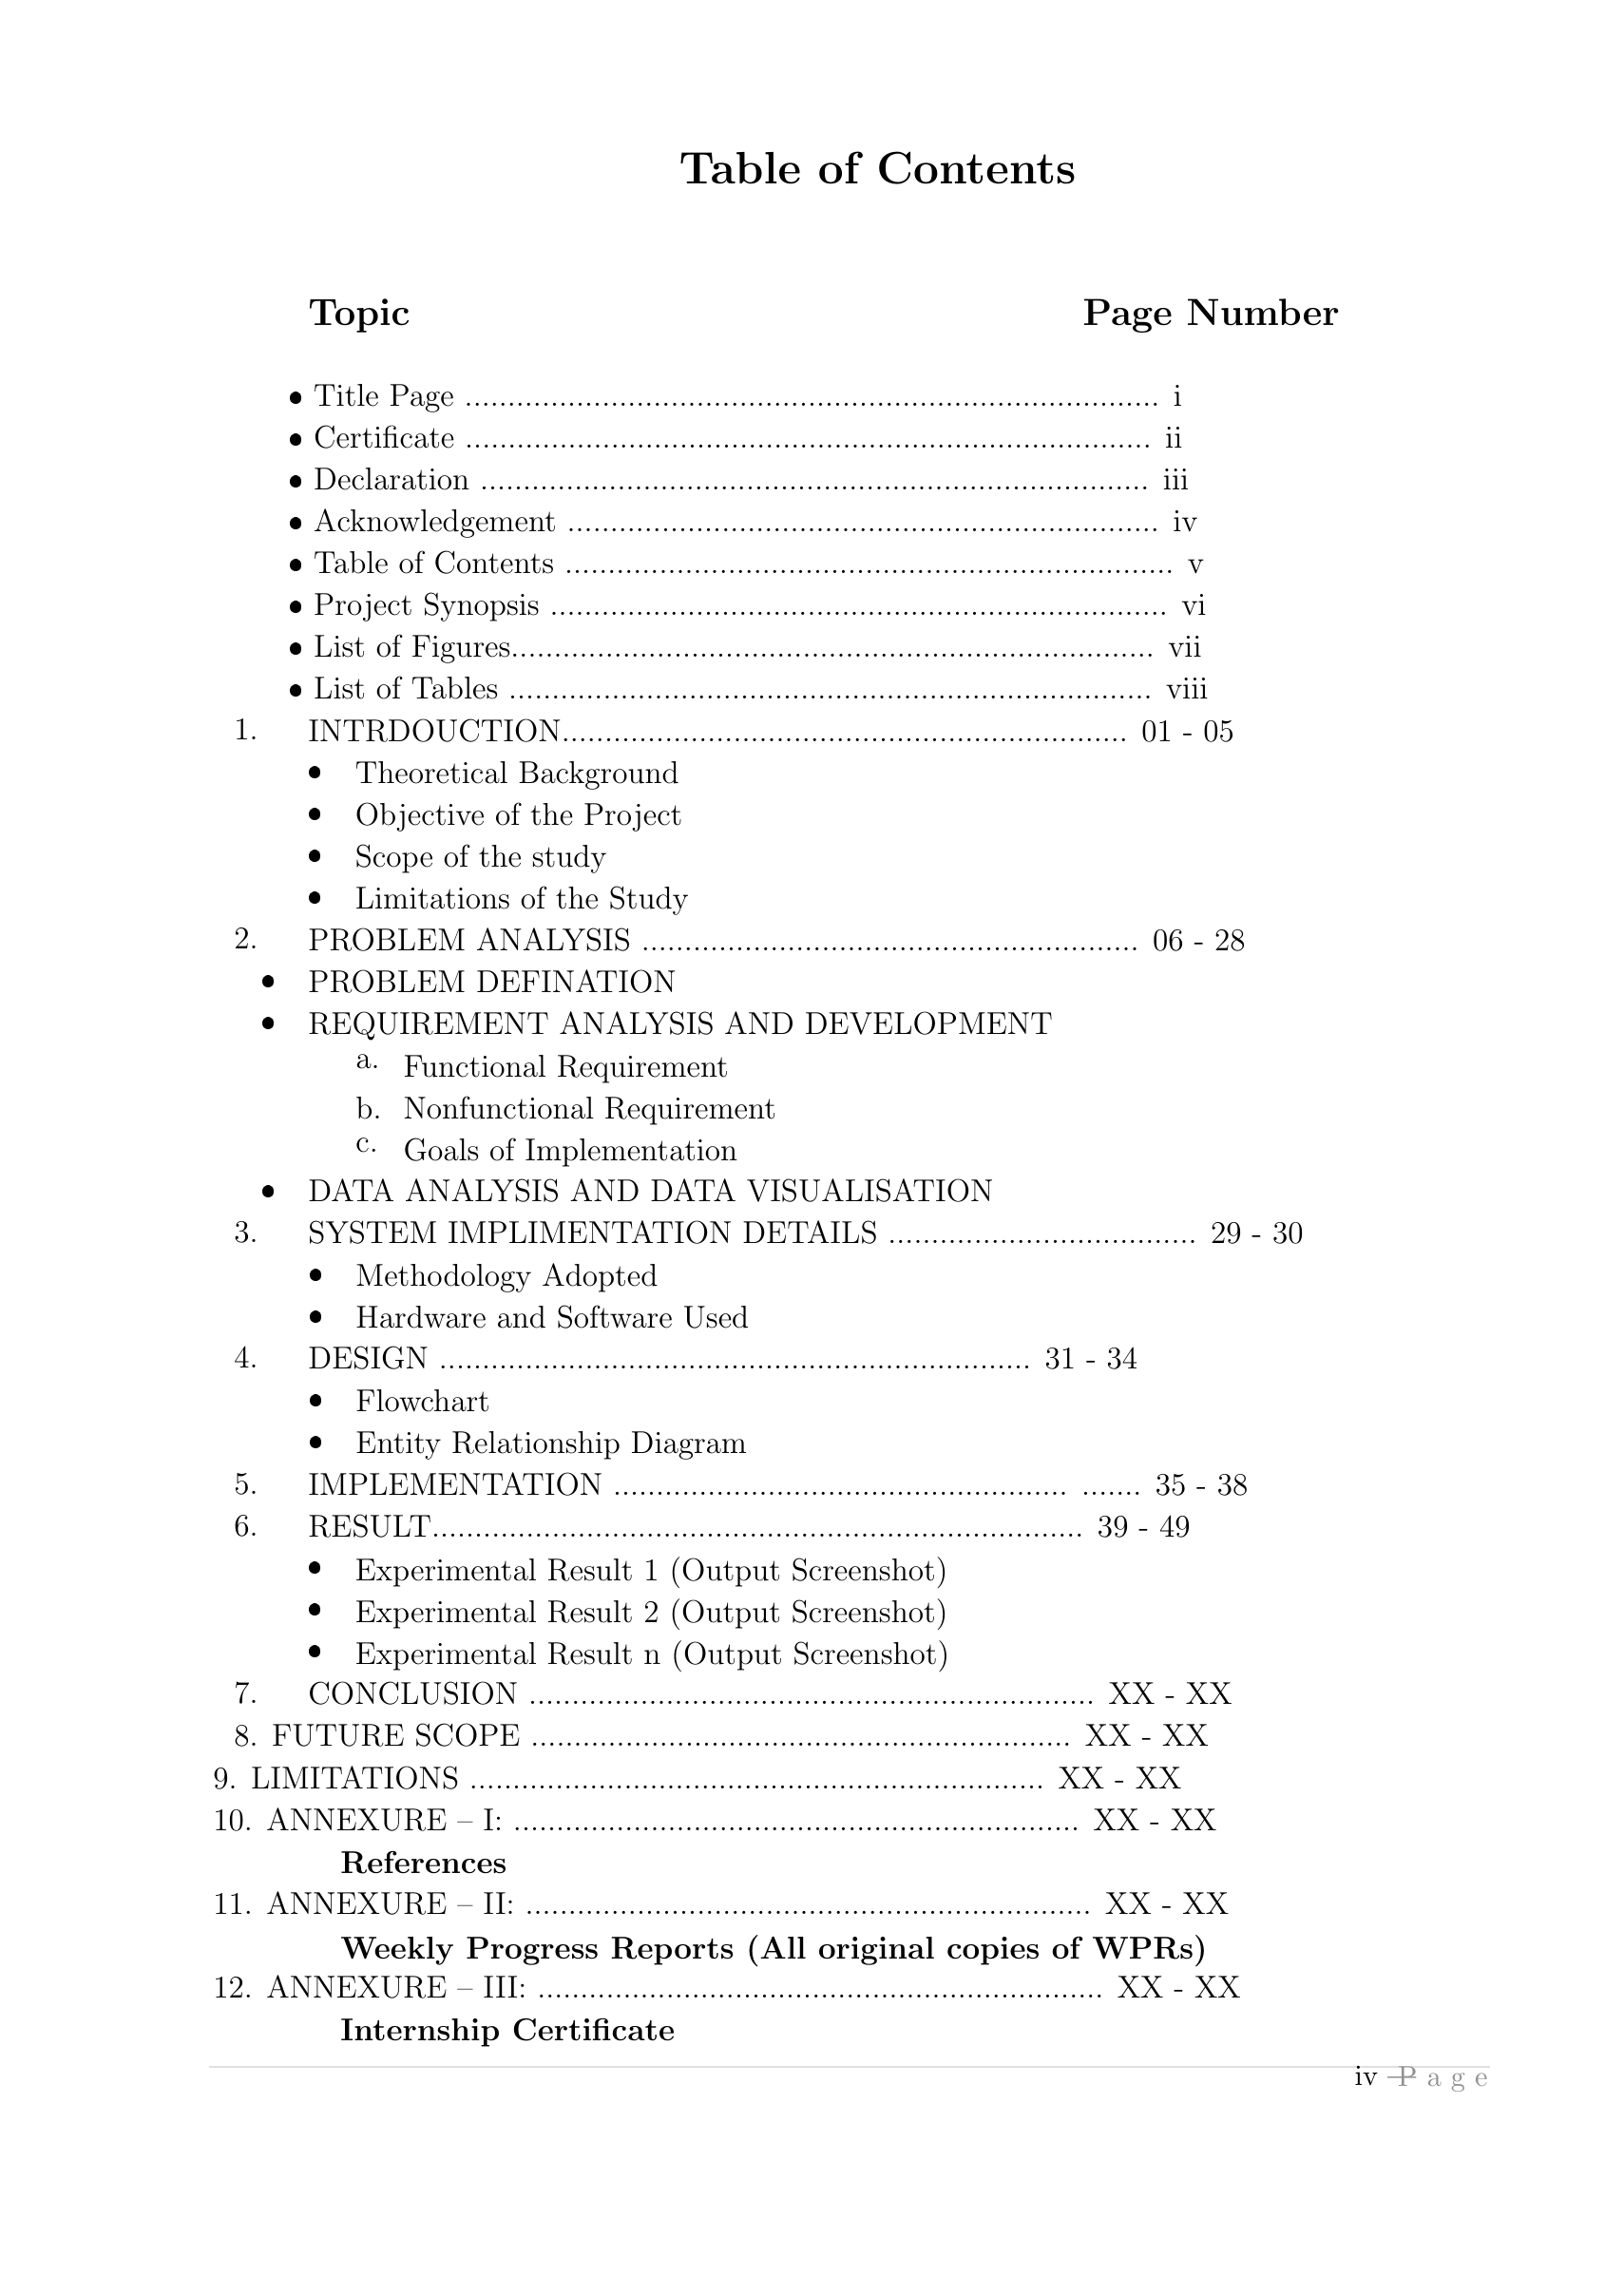
\begin{tikzpicture}[x=1bp,y=-1bp,inner sep=0pt,outer sep=0pt]
  \useasboundingbox (0,0) rectangle (595.20,841.92);
  \fill[fill=pdfcolor9] (69.38,772.78) rectangle (554.40,773.26);
  \node[anchor=north west,inner sep=0pt,outer sep=0pt] at (503.26,772.91) {{\fontsize{11.0bp}{13.2bp}\selectfont iv | }};
  \node[anchor=north west,inner sep=0pt,outer sep=0pt] at (519.58,772.91) {{\fontsize{11.0bp}{13.2bp}\selectfont \textcolor{pdfcolor1}{P a g e}}};
  \node[anchor=north west,inner sep=0pt,outer sep=0pt] at (550.14,772.91) {{\fontsize{11.0bp}{13.2bp}\selectfont   }};
  \node[anchor=north west,inner sep=0pt,outer sep=0pt] at (247.30,47.71) {{\fontsize{18.0bp}{21.6bp}\selectfont \textbf{Table of Contents }}};
  \node[anchor=north west,inner sep=0pt,outer sep=0pt] at (78.74,103.33) {{\fontsize{13.9bp}{16.7bp}\selectfont \textbf{ }}};
  \node[anchor=north west,inner sep=0pt,outer sep=0pt] at (106.85,103.33) {{\fontsize{13.9bp}{16.7bp}\selectfont \textbf{Topic  }}};
  \node[anchor=north west,inner sep=0pt,outer sep=0pt] at (178.87,103.33) {{\fontsize{13.9bp}{16.7bp}\selectfont \textbf{ }}};
  \node[anchor=north west,inner sep=0pt,outer sep=0pt] at (214.90,103.33) {{\fontsize{13.9bp}{16.7bp}\selectfont \textbf{ }}};
  \node[anchor=north west,inner sep=0pt,outer sep=0pt] at (250.90,103.33) {{\fontsize{13.9bp}{16.7bp}\selectfont \textbf{ }}};
  \node[anchor=north west,inner sep=0pt,outer sep=0pt] at (286.92,103.33) {{\fontsize{13.9bp}{16.7bp}\selectfont \textbf{ }}};
  \node[anchor=north west,inner sep=0pt,outer sep=0pt] at (322.94,103.33) {{\fontsize{13.9bp}{16.7bp}\selectfont \textbf{ }}};
  \node[anchor=north west,inner sep=0pt,outer sep=0pt] at (358.94,103.33) {{\fontsize{13.9bp}{16.7bp}\selectfont \textbf{ }}};
  \node[anchor=north west,inner sep=0pt,outer sep=0pt] at (394.97,103.33) {{\fontsize{13.9bp}{16.7bp}\selectfont \textbf{          Page Number }}};
  \node[anchor=north west,inner sep=0pt,outer sep=0pt] at (99.17,135.73) {{\fontsize{12.0bp}{14.4bp}\selectfont • Title Page .................................................................................    i }};
  \node[anchor=north west,inner sep=0pt,outer sep=0pt] at (99.17,151.57) {{\fontsize{12.0bp}{14.4bp}\selectfont • Certificate ................................................................................    ii }};
  \node[anchor=north west,inner sep=0pt,outer sep=0pt] at (99.17,167.41) {{\fontsize{12.0bp}{14.4bp}\selectfont • Declaration ..............................................................................    iii }};
  \node[anchor=north west,inner sep=0pt,outer sep=0pt] at (99.17,183.25) {{\fontsize{12.0bp}{14.4bp}\selectfont • Acknowledgement .....................................................................    iv }};
  \node[anchor=north west,inner sep=0pt,outer sep=0pt] at (99.17,199.09) {{\fontsize{12.0bp}{14.4bp}\selectfont • Table of Contents .......................................................................    v }};
  \node[anchor=north west,inner sep=0pt,outer sep=0pt] at (99.17,214.95) {{\fontsize{12.0bp}{14.4bp}\selectfont • Project Synopsis ........................................................................   vi   }};
  \node[anchor=north west,inner sep=0pt,outer sep=0pt] at (99.17,230.79) {{\fontsize{12.0bp}{14.4bp}\selectfont • List of Figures...........................................................................   vii  }};
  \node[anchor=north west,inner sep=0pt,outer sep=0pt] at (99.17,246.63) {{\fontsize{12.0bp}{14.4bp}\selectfont • List of Tables ...........................................................................   viii }};
  \node[anchor=north west,inner sep=0pt,outer sep=0pt] at (78.74,262.71) {{\fontsize{12.0bp}{14.4bp}\selectfont 1. }};
  \node[anchor=north west,inner sep=0pt,outer sep=0pt] at (106.85,262.71) {{\fontsize{12.0bp}{14.4bp}\selectfont INTRDOUCTION..................................................................   01 - 05 }};
  \node[anchor=north west,inner sep=0pt,outer sep=0pt] at (106.61,280.50) {{\fontsize{12.0bp}{14.4bp}\selectfont •}};
  \node[anchor=north west,inner sep=0pt,outer sep=0pt] at (110.93,278.29) {\textsf{{\fontsize{12.0bp}{14.4bp}\selectfont  }}};
  \node[anchor=north west,inner sep=0pt,outer sep=0pt] at (124.61,278.55) {{\fontsize{12.0bp}{14.4bp}\selectfont Theoretical Background  }};
  \node[anchor=north west,inner sep=0pt,outer sep=0pt] at (106.61,296.37) {{\fontsize{12.0bp}{14.4bp}\selectfont •}};
  \node[anchor=north west,inner sep=0pt,outer sep=0pt] at (110.93,294.16) {\textsf{{\fontsize{12.0bp}{14.4bp}\selectfont  }}};
  \node[anchor=north west,inner sep=0pt,outer sep=0pt] at (124.61,294.42) {{\fontsize{12.0bp}{14.4bp}\selectfont Objective of the Project  }};
  \node[anchor=north west,inner sep=0pt,outer sep=0pt] at (106.61,312.21) {{\fontsize{12.0bp}{14.4bp}\selectfont •}};
  \node[anchor=north west,inner sep=0pt,outer sep=0pt] at (110.93,310.00) {\textsf{{\fontsize{12.0bp}{14.4bp}\selectfont  }}};
  \node[anchor=north west,inner sep=0pt,outer sep=0pt] at (124.61,310.26) {{\fontsize{12.0bp}{14.4bp}\selectfont Scope of the study }};
  \node[anchor=north west,inner sep=0pt,outer sep=0pt] at (106.61,328.05) {{\fontsize{12.0bp}{14.4bp}\selectfont •}};
  \node[anchor=north west,inner sep=0pt,outer sep=0pt] at (110.93,325.84) {\textsf{{\fontsize{12.0bp}{14.4bp}\selectfont  }}};
  \node[anchor=north west,inner sep=0pt,outer sep=0pt] at (124.61,326.10) {{\fontsize{12.0bp}{14.4bp}\selectfont Limitations of the Study }};
  \node[anchor=north west,inner sep=0pt,outer sep=0pt] at (78.74,341.94) {{\fontsize{12.0bp}{14.4bp}\selectfont 2. }};
  \node[anchor=north west,inner sep=0pt,outer sep=0pt] at (106.85,341.94) {{\fontsize{12.0bp}{14.4bp}\selectfont PROBLEM ANALYSIS ..........................................................   06 - 28 }};
  \node[anchor=north west,inner sep=0pt,outer sep=0pt] at (88.85,359.73) {{\fontsize{12.0bp}{14.4bp}\selectfont •}};
  \node[anchor=north west,inner sep=0pt,outer sep=0pt] at (93.17,357.52) {\textsf{{\fontsize{12.0bp}{14.4bp}\selectfont  }}};
  \node[anchor=north west,inner sep=0pt,outer sep=0pt] at (106.85,357.78) {{\fontsize{12.0bp}{14.4bp}\selectfont PROBLEM DEFINATION }};
  \node[anchor=north west,inner sep=0pt,outer sep=0pt] at (88.85,375.59) {{\fontsize{12.0bp}{14.4bp}\selectfont •}};
  \node[anchor=north west,inner sep=0pt,outer sep=0pt] at (93.17,373.38) {\textsf{{\fontsize{12.0bp}{14.4bp}\selectfont  }}};
  \node[anchor=north west,inner sep=0pt,outer sep=0pt] at (106.85,373.64) {{\fontsize{12.0bp}{14.4bp}\selectfont REQUIREMENT ANALYSIS AND DEVELOPMENT }};
  \node[anchor=north west,inner sep=0pt,outer sep=0pt] at (124.85,389.72) {{\fontsize{12.0bp}{14.4bp}\selectfont a.}};
  \node[anchor=north west,inner sep=0pt,outer sep=0pt] at (133.25,389.46) {\textsf{{\fontsize{12.0bp}{14.4bp}\selectfont  }}};
  \node[anchor=north west,inner sep=0pt,outer sep=0pt] at (142.87,389.72) {{\fontsize{12.0bp}{14.4bp}\selectfont Functional Requirement }};
  \node[anchor=north west,inner sep=0pt,outer sep=0pt] at (124.85,405.56) {{\fontsize{12.0bp}{14.4bp}\selectfont b.}};
  \node[anchor=north west,inner sep=0pt,outer sep=0pt] at (133.97,405.30) {\textsf{{\fontsize{12.0bp}{14.4bp}\selectfont  }}};
  \node[anchor=north west,inner sep=0pt,outer sep=0pt] at (142.87,405.56) {{\fontsize{12.0bp}{14.4bp}\selectfont Nonfunctional Requirement }};
  \node[anchor=north west,inner sep=0pt,outer sep=0pt] at (124.85,421.40) {{\fontsize{12.0bp}{14.4bp}\selectfont c.}};
  \node[anchor=north west,inner sep=0pt,outer sep=0pt] at (133.25,421.14) {\textsf{{\fontsize{12.0bp}{14.4bp}\selectfont  }}};
  \node[anchor=north west,inner sep=0pt,outer sep=0pt] at (142.87,421.40) {{\fontsize{12.0bp}{14.4bp}\selectfont Goals of Implementation }};
  \node[anchor=north west,inner sep=0pt,outer sep=0pt] at (88.85,439.19) {{\fontsize{12.0bp}{14.4bp}\selectfont •}};
  \node[anchor=north west,inner sep=0pt,outer sep=0pt] at (93.17,436.98) {\textsf{{\fontsize{12.0bp}{14.4bp}\selectfont  }}};
  \node[anchor=north west,inner sep=0pt,outer sep=0pt] at (106.85,437.24) {{\fontsize{12.0bp}{14.4bp}\selectfont DATA ANALYSIS AND DATA VISUALISATION }};
  \node[anchor=north west,inner sep=0pt,outer sep=0pt] at (78.74,453.08) {{\fontsize{12.0bp}{14.4bp}\selectfont 3. }};
  \node[anchor=north west,inner sep=0pt,outer sep=0pt] at (106.85,453.08) {{\fontsize{12.0bp}{14.4bp}\selectfont SYSTEM IMPLIMENTATION DETAILS ....................................  29 - 30 }};
  \node[anchor=north west,inner sep=0pt,outer sep=0pt] at (106.85,470.89) {{\fontsize{12.0bp}{14.4bp}\selectfont •}};
  \node[anchor=north west,inner sep=0pt,outer sep=0pt] at (111.17,468.68) {\textsf{{\fontsize{12.0bp}{14.4bp}\selectfont  }}};
  \node[anchor=north west,inner sep=0pt,outer sep=0pt] at (124.85,468.94) {{\fontsize{12.0bp}{14.4bp}\selectfont Methodology Adopted }};
  \node[anchor=north west,inner sep=0pt,outer sep=0pt] at (106.85,486.73) {{\fontsize{12.0bp}{14.4bp}\selectfont •}};
  \node[anchor=north west,inner sep=0pt,outer sep=0pt] at (111.17,484.52) {\textsf{{\fontsize{12.0bp}{14.4bp}\selectfont  }}};
  \node[anchor=north west,inner sep=0pt,outer sep=0pt] at (124.85,484.78) {{\fontsize{12.0bp}{14.4bp}\selectfont Hardware and Software Used }};
  \node[anchor=north west,inner sep=0pt,outer sep=0pt] at (78.74,500.62) {{\fontsize{12.0bp}{14.4bp}\selectfont 4. }};
  \node[anchor=north west,inner sep=0pt,outer sep=0pt] at (106.85,500.62) {{\fontsize{12.0bp}{14.4bp}\selectfont DESIGN           .....................................................................  31 - 34 }};
  \node[anchor=north west,inner sep=0pt,outer sep=0pt] at (106.85,518.41) {{\fontsize{12.0bp}{14.4bp}\selectfont •}};
  \node[anchor=north west,inner sep=0pt,outer sep=0pt] at (111.17,516.20) {\textsf{{\fontsize{12.0bp}{14.4bp}\selectfont  }}};
  \node[anchor=north west,inner sep=0pt,outer sep=0pt] at (124.85,516.46) {{\fontsize{12.0bp}{14.4bp}\selectfont Flowchart }};
  \node[anchor=north west,inner sep=0pt,outer sep=0pt] at (106.85,534.49) {{\fontsize{12.0bp}{14.4bp}\selectfont •}};
  \node[anchor=north west,inner sep=0pt,outer sep=0pt] at (111.17,532.28) {\textsf{{\fontsize{12.0bp}{14.4bp}\selectfont  }}};
  \node[anchor=north west,inner sep=0pt,outer sep=0pt] at (124.85,532.54) {{\fontsize{12.0bp}{14.4bp}\selectfont Entity Relationship Diagram }};
  \node[anchor=north west,inner sep=0pt,outer sep=0pt] at (78.74,548.41) {{\fontsize{12.0bp}{14.4bp}\selectfont 5. }};
  \node[anchor=north west,inner sep=0pt,outer sep=0pt] at (106.85,548.41) {{\fontsize{12.0bp}{14.4bp}\selectfont IMPLEMENTATION ..................................................... .......   35 - 38 }};
  \node[anchor=north west,inner sep=0pt,outer sep=0pt] at (78.74,564.25) {{\fontsize{12.0bp}{14.4bp}\selectfont 6. }};
  \node[anchor=north west,inner sep=0pt,outer sep=0pt] at (106.85,564.25) {{\fontsize{12.0bp}{14.4bp}\selectfont RESULT............................................................................    39 - 49 }};
  \node[anchor=north west,inner sep=0pt,outer sep=0pt] at (106.61,582.04) {{\fontsize{12.0bp}{14.4bp}\selectfont •}};
  \node[anchor=north west,inner sep=0pt,outer sep=0pt] at (110.93,579.83) {\textsf{{\fontsize{12.0bp}{14.4bp}\selectfont  }}};
  \node[anchor=north west,inner sep=0pt,outer sep=0pt] at (124.61,580.09) {{\fontsize{12.0bp}{14.4bp}\selectfont Experimental Result 1 (Output Screenshot) }};
  \node[anchor=north west,inner sep=0pt,outer sep=0pt] at (106.61,597.88) {{\fontsize{12.0bp}{14.4bp}\selectfont •}};
  \node[anchor=north west,inner sep=0pt,outer sep=0pt] at (110.93,595.67) {\textsf{{\fontsize{12.0bp}{14.4bp}\selectfont  }}};
  \node[anchor=north west,inner sep=0pt,outer sep=0pt] at (124.61,595.93) {{\fontsize{12.0bp}{14.4bp}\selectfont Experimental Result 2 (Output Screenshot) }};
  \node[anchor=north west,inner sep=0pt,outer sep=0pt] at (106.61,613.72) {{\fontsize{12.0bp}{14.4bp}\selectfont •}};
  \node[anchor=north west,inner sep=0pt,outer sep=0pt] at (110.93,611.51) {\textsf{{\fontsize{12.0bp}{14.4bp}\selectfont  }}};
  \node[anchor=north west,inner sep=0pt,outer sep=0pt] at (124.61,611.77) {{\fontsize{12.0bp}{14.4bp}\selectfont Experimental Result n (Output Screenshot) }};
  \node[anchor=north west,inner sep=0pt,outer sep=0pt] at (78.74,627.61) {{\fontsize{12.0bp}{14.4bp}\selectfont 7. }};
  \node[anchor=north west,inner sep=0pt,outer sep=0pt] at (106.85,627.61) {{\fontsize{12.0bp}{14.4bp}\selectfont CONCLUSION ..................................................................    XX - XX }};
  \node[anchor=north west,inner sep=0pt,outer sep=0pt] at (78.74,643.47) {{\fontsize{12.0bp}{14.4bp}\selectfont 8.      FUTURE SCOPE ...............................................................     XX - XX }};
  \node[anchor=north west,inner sep=0pt,outer sep=0pt] at (70.82,659.55) {{\fontsize{12.0bp}{14.4bp}\selectfont   9.      LIMITATIONS ...................................................................    XX - XX }};
  \node[anchor=north west,inner sep=0pt,outer sep=0pt] at (70.82,675.39) {{\fontsize{12.0bp}{14.4bp}\selectfont  10.     ANNEXURE -- I:  ..................................................................  XX - XX      }};
  \node[anchor=north west,inner sep=0pt,outer sep=0pt] at (70.82,691.23) {{\fontsize{12.0bp}{14.4bp}\selectfont                 }};
  \node[anchor=north west,inner sep=0pt,outer sep=0pt] at (119.09,691.34) {{\fontsize{12.0bp}{14.4bp}\selectfont \textbf{References  }}};
  \node[anchor=north west,inner sep=0pt,outer sep=0pt] at (70.82,707.07) {{\fontsize{12.0bp}{14.4bp}\selectfont  11.     ANNEXURE -- II:  ..................................................................  XX - XX      }};
  \node[anchor=north west,inner sep=0pt,outer sep=0pt] at (70.82,722.94) {{\fontsize{12.0bp}{14.4bp}\selectfont                 }};
  \node[anchor=north west,inner sep=0pt,outer sep=0pt] at (119.09,723.05) {{\fontsize{12.0bp}{14.4bp}\selectfont \textbf{Weekly Progress Reports (All original copies of WPRs)  }}};
  \node[anchor=north west,inner sep=0pt,outer sep=0pt] at (70.82,738.78) {{\fontsize{12.0bp}{14.4bp}\selectfont 12.     ANNEXURE -- III:  ..................................................................  XX - XX      }};
  \node[anchor=north west,inner sep=0pt,outer sep=0pt] at (70.82,754.62) {{\fontsize{12.0bp}{14.4bp}\selectfont                 }};
  \node[anchor=north west,inner sep=0pt,outer sep=0pt] at (119.09,754.73) {{\fontsize{12.0bp}{14.4bp}\selectfont \textbf{Internship Certificate }}};
\end{tikzpicture}
\newpage
\noindent
\begin{tikzpicture}[x=1bp,y=-1bp,inner sep=0pt,outer sep=0pt]
  \useasboundingbox (0,0) rectangle (595.20,841.92);
  \fill[fill=pdfcolor9] (69.38,772.78) rectangle (554.40,773.26);
  \fill[fill=black] (69.38,106.10) rectangle (554.40,106.82);
  \fill[fill=black] (243.22,121.22) rectangle (380.57,122.66);
  \fill[fill=black] (87.41,298.42) rectangle (554.40,299.14);
  \fill[fill=black] (251.86,322.66) rectangle (371.93,324.10);
  \node[anchor=north west,inner sep=0pt] at (224.15,18.45) {
\includegraphics[width=175.35bp,height=63.45bp]{images/image_p6_2.png}};
  \node[anchor=north west,inner sep=0pt,outer sep=0pt] at (506.38,772.91) {{\fontsize{11.0bp}{13.2bp}\selectfont v | }};
  \node[anchor=north west,inner sep=0pt,outer sep=0pt] at (519.58,772.91) {{\fontsize{11.0bp}{13.2bp}\selectfont \textcolor{pdfcolor1}{P a g e}}};
  \node[anchor=north west,inner sep=0pt,outer sep=0pt] at (550.14,772.91) {{\fontsize{11.0bp}{13.2bp}\selectfont   }};
  \node[anchor=north west,inner sep=0pt,outer sep=0pt] at (205.30,85.95) {{\fontsize{16.1bp}{19.3bp}\selectfont \textbf{THE DEPARTMENT OF CSE }}};
  \node[anchor=north west,inner sep=0pt,outer sep=0pt] at (243.22,105.25) {{\fontsize{13.9bp}{16.7bp}\selectfont \textbf{PROJECT SYNOPSIS }}};
  \node[anchor=north west,inner sep=0pt,outer sep=0pt] at (70.82,129.60) {{\fontsize{12.0bp}{14.4bp}\selectfont \textbf{Student Name: Abhishek Chatterjee, Shivani Deonath, Jiten kr Sarkhel  }}};
  \node[anchor=north west,inner sep=0pt,outer sep=0pt] at (70.82,150.48) {{\fontsize{12.0bp}{14.4bp}\selectfont \textbf{Enrollment No.: SBU221026, SBU221482, SBU220845 }}};
  \node[anchor=north west,inner sep=0pt,outer sep=0pt] at (70.82,171.12) {{\fontsize{12.0bp}{14.4bp}\selectfont \textbf{Program \& Branch: BTech CSE (AI\&ML, DS\&CC) }}};
  \node[anchor=north west,inner sep=0pt,outer sep=0pt] at (70.82,191.76) {{\fontsize{12.0bp}{14.4bp}\selectfont \textbf{Batch: 2022-2026, Semester: 6th, Section:  A, D }}};
  \node[anchor=north west,inner sep=0pt,outer sep=0pt] at (70.82,212.42) {{\fontsize{12.0bp}{14.4bp}\selectfont \textbf{Academic Session: Even Semester 2024-25 }}};
  \node[anchor=north west,inner sep=0pt,outer sep=0pt] at (70.82,233.30) {{\fontsize{12.0bp}{14.4bp}\selectfont \textbf{Project Guide Details: }}};
  \node[anchor=north west,inner sep=0pt,outer sep=0pt] at (88.85,255.13) {{\fontsize{12.0bp}{14.4bp}\selectfont •}};
  \node[anchor=north west,inner sep=0pt,outer sep=0pt] at (94.37,254.29) {\textsf{{\fontsize{12.0bp}{14.4bp}\selectfont  }}};
  \node[anchor=north west,inner sep=0pt,outer sep=0pt] at (106.85,254.66) {{\fontsize{12.0bp}{14.4bp}\selectfont \textbf{Guide Name: Dr. Dipti Kumari }}};
  \node[anchor=north west,inner sep=0pt,outer sep=0pt] at (88.85,276.73) {{\fontsize{12.0bp}{14.4bp}\selectfont •}};
  \node[anchor=north west,inner sep=0pt,outer sep=0pt] at (94.37,275.89) {\textsf{{\fontsize{12.0bp}{14.4bp}\selectfont  }}};
  \node[anchor=north west,inner sep=0pt,outer sep=0pt] at (106.85,276.26) {{\fontsize{12.0bp}{14.4bp}\selectfont \textbf{Designation: Associate Professor, CSE, SBU }}};
  \node[anchor=north west,inner sep=0pt,outer sep=0pt] at (251.86,306.69) {{\fontsize{13.9bp}{16.7bp}\selectfont \textbf{Project Information }}};
  \node[anchor=north west,inner sep=0pt,outer sep=0pt] at (70.82,331.29) {{\fontsize{11.0bp}{13.2bp}\selectfont \textbf{1. Course Title:}}};
  \node[anchor=north west,inner sep=0pt,outer sep=0pt] at (144.07,331.19) {{\fontsize{11.0bp}{13.2bp}\selectfont  }};
  \node[anchor=north west,inner sep=0pt,outer sep=0pt] at (146.95,331.29) {{\fontsize{11.0bp}{13.2bp}\selectfont \textbf{Project Stage-I (Mini Project/ Industrial Training) }}};
  \node[anchor=north west,inner sep=0pt,outer sep=0pt] at (70.82,350.25) {{\fontsize{11.0bp}{13.2bp}\selectfont \textbf{2. Courses Code: CSE-601-P1                                              }}};
  \node[anchor=north west,inner sep=0pt,outer sep=0pt] at (70.82,369.21) {{\fontsize{11.0bp}{13.2bp}\selectfont \textbf{3. Credit Unit: 2 }}};
  \node[anchor=north west,inner sep=0pt,outer sep=0pt] at (70.82,388.19) {{\fontsize{11.0bp}{13.2bp}\selectfont \textbf{4. Project/ Internship Duration:  }}};
  \node[anchor=north west,inner sep=0pt,outer sep=0pt] at (124.85,408.30) {{\fontsize{11.0bp}{13.2bp}\selectfont •}};
  \node[anchor=north west,inner sep=0pt,outer sep=0pt] at (129.89,407.53) {\textsf{{\fontsize{11.0bp}{13.2bp}\selectfont  }}};
  \node[anchor=north west,inner sep=0pt,outer sep=0pt] at (142.87,407.87) {{\fontsize{11.0bp}{13.2bp}\selectfont \textbf{Date of Project Commencement: 21}}};
  \node[anchor=north west,inner sep=0pt,outer sep=0pt] at (310.46,407.09) {{\fontsize{7.0bp}{8.4bp}\selectfont \textbf{st}}};
  \node[anchor=north west,inner sep=0pt,outer sep=0pt] at (315.50,407.87) {{\fontsize{11.0bp}{13.2bp}\selectfont \textbf{ March, 2024 }}};
  \node[anchor=north west,inner sep=0pt,outer sep=0pt] at (124.85,427.98) {{\fontsize{11.0bp}{13.2bp}\selectfont •}};
  \node[anchor=north west,inner sep=0pt,outer sep=0pt] at (129.89,427.21) {\textsf{{\fontsize{11.0bp}{13.2bp}\selectfont  }}};
  \node[anchor=north west,inner sep=0pt,outer sep=0pt] at (142.87,427.55) {{\fontsize{11.0bp}{13.2bp}\selectfont \textbf{Date of Project Completion: 21}}};
  \node[anchor=north west,inner sep=0pt,outer sep=0pt] at (289.08,426.77) {{\fontsize{7.0bp}{8.4bp}\selectfont \textbf{st}}};
  \node[anchor=north west,inner sep=0pt,outer sep=0pt] at (294.12,427.55) {{\fontsize{11.0bp}{13.2bp}\selectfont \textbf{ April, 2025 }}};
  \node[anchor=north west,inner sep=0pt,outer sep=0pt] at (70.82,446.51) {{\fontsize{11.0bp}{13.2bp}\selectfont \textbf{5. Approved Project Title (to be duly approved by the Project Guide): }}};
  \node[anchor=north west,inner sep=0pt,outer sep=0pt] at (70.82,465.49) {{\fontsize{11.0bp}{13.2bp}\selectfont \textbf{ }}};
  \node[anchor=north west,inner sep=0pt,outer sep=0pt] at (106.85,467.18) {{\fontsize{11.0bp}{13.2bp}\selectfont \textbf{“Credit Card Fraud Detection using Machine Learning”}}};
  \node[anchor=north west,inner sep=0pt,outer sep=0pt] at (372.65,465.39) {{\fontsize{11.0bp}{13.2bp}\selectfont  }};
  \node[anchor=north west,inner sep=0pt,outer sep=0pt] at (70.82,478.21) {{\fontsize{11.0bp}{13.2bp}\selectfont \textbf{6. Objectives: }}};
  \node[anchor=north west,inner sep=0pt,outer sep=0pt] at (137.81,478.11) {{\fontsize{11.0bp}{13.2bp}\selectfont  }};
  \node[anchor=north west,inner sep=0pt,outer sep=0pt] at (70.82,497.07) {{\fontsize{11.0bp}{13.2bp}\selectfont Develop a machine learning model for real-time credit card fraud detection using classification and anomaly }};
  \node[anchor=north west,inner sep=0pt,outer sep=0pt] at (70.82,516.03) {{\fontsize{11.0bp}{13.2bp}\selectfont detection techniques, handling class imbalance with SMOTE. Evaluate performance using metrics like ROC-}};
  \node[anchor=north west,inner sep=0pt,outer sep=0pt] at (70.82,534.99) {{\fontsize{11.0bp}{13.2bp}\selectfont AUC and F1-score, and deploy with a user-friendly interface for practical financial security applications. }};
  \node[anchor=north west,inner sep=0pt,outer sep=0pt] at (70.82,554.08) {{\fontsize{11.0bp}{13.2bp}\selectfont \textbf{7. Methodology to be adopted: }}};
  \node[anchor=north west,inner sep=0pt,outer sep=0pt] at (88.85,574.43) {{\fontsize{11.0bp}{13.2bp}\selectfont •}};
  \node[anchor=north west,inner sep=0pt,outer sep=0pt] at (93.89,573.66) {\textsf{{\fontsize{11.0bp}{13.2bp}\selectfont  }}};
  \node[anchor=north west,inner sep=0pt,outer sep=0pt] at (106.85,574.00) {{\fontsize{11.0bp}{13.2bp}\selectfont \textbf{Data Collection \& Preprocessing:}}};
  \node[anchor=north west,inner sep=0pt,outer sep=0pt] at (264.36,573.90) {{\fontsize{11.0bp}{13.2bp}\selectfont  Used Kaggle data, cleaned, scaled, applied SMOTE. }};
  \node[anchor=north west,inner sep=0pt,outer sep=0pt] at (88.85,594.11) {{\fontsize{11.0bp}{13.2bp}\selectfont •}};
  \node[anchor=north west,inner sep=0pt,outer sep=0pt] at (93.89,593.34) {\textsf{{\fontsize{11.0bp}{13.2bp}\selectfont  }}};
  \node[anchor=north west,inner sep=0pt,outer sep=0pt] at (106.85,593.68) {{\fontsize{11.0bp}{13.2bp}\selectfont \textbf{Model Building \& Evaluation:}}};
  \node[anchor=north west,inner sep=0pt,outer sep=0pt] at (249.70,593.58) {{\fontsize{11.0bp}{13.2bp}\selectfont  Trained Random Forest, evaluated with key metrics. }};
  \node[anchor=north west,inner sep=0pt,outer sep=0pt] at (88.85,613.79) {{\fontsize{11.0bp}{13.2bp}\selectfont •}};
  \node[anchor=north west,inner sep=0pt,outer sep=0pt] at (93.89,613.02) {\textsf{{\fontsize{11.0bp}{13.2bp}\selectfont  }}};
  \node[anchor=north west,inner sep=0pt,outer sep=0pt] at (106.85,613.36) {{\fontsize{11.0bp}{13.2bp}\selectfont \textbf{Deployment \& Documentation:}}};
  \node[anchor=north west,inner sep=0pt,outer sep=0pt] at (254.28,613.26) {{\fontsize{11.0bp}{13.2bp}\selectfont  Built Streamlit web app, documented project. }};
  \node[anchor=north west,inner sep=0pt,outer sep=0pt] at (70.82,632.58) {{\fontsize{11.0bp}{13.2bp}\selectfont \textbf{8. Brief Summary of the project: }}};
  \node[anchor=north west,inner sep=0pt,outer sep=0pt] at (70.82,651.44) {{\fontsize{11.0bp}{13.2bp}\selectfont This project detects credit card fraud using anonymized, imbalanced data by applying preprocessing, }};
  \node[anchor=north west,inner sep=0pt,outer sep=0pt] at (70.82,670.40) {{\fontsize{11.0bp}{13.2bp}\selectfont SMOTE oversampling, and a Random Forest model. It is evaluated with key metrics and deployed through }};
  \node[anchor=north west,inner sep=0pt,outer sep=0pt] at (70.82,689.36) {{\fontsize{11.0bp}{13.2bp}\selectfont an easy-to-use interface to help reduce fraud. }};
  \node[anchor=north west,inner sep=0pt,outer sep=0pt] at (70.82,746.37) {{\fontsize{11.0bp}{13.2bp}\selectfont \textbf{Signature with date }}};
  \node[anchor=north west,inner sep=0pt,outer sep=0pt] at (178.87,746.37) {{\fontsize{11.0bp}{13.2bp}\selectfont \textbf{ }}};
  \node[anchor=north west,inner sep=0pt,outer sep=0pt] at (214.90,746.37) {{\fontsize{11.0bp}{13.2bp}\selectfont \textbf{   Signature of Industry Guide, if any  }}};
  \node[anchor=north west,inner sep=0pt,outer sep=0pt] at (430.99,746.37) {{\fontsize{11.0bp}{13.2bp}\selectfont \textbf{     Signature with date }}};
\end{tikzpicture}
\newpage
\noindent
\begin{tikzpicture}[x=1bp,y=-1bp,inner sep=0pt,outer sep=0pt]
  \useasboundingbox (0,0) rectangle (595.20,841.92);
  \fill[fill=pdfcolor9] (69.38,772.78) rectangle (554.40,773.26);
  \node[anchor=north west,inner sep=0pt,outer sep=0pt] at (503.26,772.91) {{\fontsize{11.0bp}{13.2bp}\selectfont vi | }};
  \node[anchor=north west,inner sep=0pt,outer sep=0pt] at (519.58,772.91) {{\fontsize{11.0bp}{13.2bp}\selectfont \textcolor{pdfcolor1}{P a g e}}};
  \node[anchor=north west,inner sep=0pt,outer sep=0pt] at (550.14,772.91) {{\fontsize{11.0bp}{13.2bp}\selectfont   }};
  \node[anchor=north west,inner sep=0pt,outer sep=0pt] at (70.82,48.39) {{\fontsize{11.0bp}{13.2bp}\selectfont    (Student) }};
  \node[anchor=north west,inner sep=0pt,outer sep=0pt] at (142.87,48.39) {{\fontsize{11.0bp}{13.2bp}\selectfont  }};
  \node[anchor=north west,inner sep=0pt,outer sep=0pt] at (178.87,48.39) {{\fontsize{11.0bp}{13.2bp}\selectfont  }};
  \node[anchor=north west,inner sep=0pt,outer sep=0pt] at (214.90,48.39) {{\fontsize{11.0bp}{13.2bp}\selectfont  }};
  \node[anchor=north west,inner sep=0pt,outer sep=0pt] at (250.90,48.39) {{\fontsize{11.0bp}{13.2bp}\selectfont  }};
  \node[anchor=north west,inner sep=0pt,outer sep=0pt] at (286.92,48.39) {{\fontsize{11.0bp}{13.2bp}\selectfont  }};
  \node[anchor=north west,inner sep=0pt,outer sep=0pt] at (322.94,48.39) {{\fontsize{11.0bp}{13.2bp}\selectfont  }};
  \node[anchor=north west,inner sep=0pt,outer sep=0pt] at (358.94,48.39) {{\fontsize{11.0bp}{13.2bp}\selectfont  }};
  \node[anchor=north west,inner sep=0pt,outer sep=0pt] at (394.97,48.39) {{\fontsize{11.0bp}{13.2bp}\selectfont  }};
  \node[anchor=north west,inner sep=0pt,outer sep=0pt] at (430.99,48.39) {{\fontsize{11.0bp}{13.2bp}\selectfont           (Project Guide) }};
  \node[anchor=north west,inner sep=0pt,outer sep=0pt] at (268.44,67.57) {{\fontsize{13.9bp}{16.7bp}\selectfont \textbf{List of Figures }}};
  \node[anchor=north west,inner sep=0pt,outer sep=0pt] at (78.74,90.69) {{\fontsize{10.1bp}{12.1bp}\selectfont  }};
  \node[anchor=north west,inner sep=0pt,outer sep=0pt] at (78.74,106.66) {{\fontsize{12.0bp}{14.4bp}\selectfont 1.}};
  \node[anchor=north west,inner sep=0pt,outer sep=0pt] at (87.89,106.40) {\textsf{{\fontsize{12.0bp}{14.4bp}\selectfont  }}};
  \node[anchor=north west,inner sep=0pt,outer sep=0pt] at (107.57,106.66) {{\fontsize{12.0bp}{14.4bp}\selectfont Xxxxxxx }};
  \node[anchor=north west,inner sep=0pt,outer sep=0pt] at (152.95,106.66) {{\fontsize{12.0bp}{14.4bp}\selectfont ................................................................................................................ }};
  \node[anchor=north west,inner sep=0pt,outer sep=0pt] at (503.50,106.66) {{\fontsize{12.0bp}{14.4bp}\selectfont  XX }};
  \node[anchor=north west,inner sep=0pt,outer sep=0pt] at (78.74,127.33) {{\fontsize{12.0bp}{14.4bp}\selectfont 2.}};
  \node[anchor=north west,inner sep=0pt,outer sep=0pt] at (87.89,127.07) {\textsf{{\fontsize{12.0bp}{14.4bp}\selectfont  }}};
  \node[anchor=north west,inner sep=0pt,outer sep=0pt] at (107.57,127.33) {{\fontsize{12.0bp}{14.4bp}\selectfont Xxxxxxxx }};
  \node[anchor=north west,inner sep=0pt,outer sep=0pt] at (159.19,127.33) {{\fontsize{12.0bp}{14.4bp}\selectfont ............................................................................................................... }};
  \node[anchor=north west,inner sep=0pt,outer sep=0pt] at (506.62,127.33) {{\fontsize{12.0bp}{14.4bp}\selectfont XX }};
  \node[anchor=north west,inner sep=0pt,outer sep=0pt] at (78.74,147.97) {{\fontsize{12.0bp}{14.4bp}\selectfont 3.}};
  \node[anchor=north west,inner sep=0pt,outer sep=0pt] at (87.89,147.71) {\textsf{{\fontsize{12.0bp}{14.4bp}\selectfont  }}};
  \node[anchor=north west,inner sep=0pt,outer sep=0pt] at (107.57,147.97) {{\fontsize{12.0bp}{14.4bp}\selectfont Xxxx }};
\end{tikzpicture}
\newpage
\noindent
\begin{tikzpicture}[x=1bp,y=-1bp,inner sep=0pt,outer sep=0pt]
  \useasboundingbox (0,0) rectangle (595.20,841.92);
  \fill[fill=pdfcolor9] (69.38,772.78) rectangle (554.40,773.26);
  \node[anchor=north west,inner sep=0pt,outer sep=0pt] at (500.14,772.91) {{\fontsize{11.0bp}{13.2bp}\selectfont vii | }};
  \node[anchor=north west,inner sep=0pt,outer sep=0pt] at (519.34,772.91) {{\fontsize{11.0bp}{13.2bp}\selectfont \textcolor{pdfcolor1}{P a g e}}};
  \node[anchor=north west,inner sep=0pt,outer sep=0pt] at (550.13,772.91) {{\fontsize{11.0bp}{13.2bp}\selectfont   }};
  \node[anchor=north west,inner sep=0pt,outer sep=0pt] at (276.84,89.49) {{\fontsize{12.0bp}{14.4bp}\selectfont \textbf{List of Tables }}};
  \node[anchor=north west,inner sep=0pt,outer sep=0pt] at (70.82,130.69) {{\fontsize{12.0bp}{14.4bp}\selectfont 1. }};
  \node[anchor=north west,inner sep=0pt,outer sep=0pt] at (107.57,130.69) {{\fontsize{12.0bp}{14.4bp}\selectfont Xxxxxxx }};
  \node[anchor=north west,inner sep=0pt,outer sep=0pt] at (152.95,130.69) {{\fontsize{12.0bp}{14.4bp}\selectfont ................................................................................................................ }};
  \node[anchor=north west,inner sep=0pt,outer sep=0pt] at (503.50,130.69) {{\fontsize{12.0bp}{14.4bp}\selectfont  XX }};
  \node[anchor=north west,inner sep=0pt,outer sep=0pt] at (70.82,151.33) {{\fontsize{12.0bp}{14.4bp}\selectfont 2. }};
  \node[anchor=north west,inner sep=0pt,outer sep=0pt] at (107.57,151.33) {{\fontsize{12.0bp}{14.4bp}\selectfont Xxxxxxxx }};
  \node[anchor=north west,inner sep=0pt,outer sep=0pt] at (159.19,151.33) {{\fontsize{12.0bp}{14.4bp}\selectfont ............................................................................................................... }};
  \node[anchor=north west,inner sep=0pt,outer sep=0pt] at (506.62,151.33) {{\fontsize{12.0bp}{14.4bp}\selectfont XX }};
  \node[anchor=north west,inner sep=0pt,outer sep=0pt] at (70.82,171.73) {{\fontsize{12.0bp}{14.4bp}\selectfont 3. }};
  \node[anchor=north west,inner sep=0pt,outer sep=0pt] at (107.57,171.73) {{\fontsize{12.0bp}{14.4bp}\selectfont  }};
\end{tikzpicture}
\newpage
\noindent
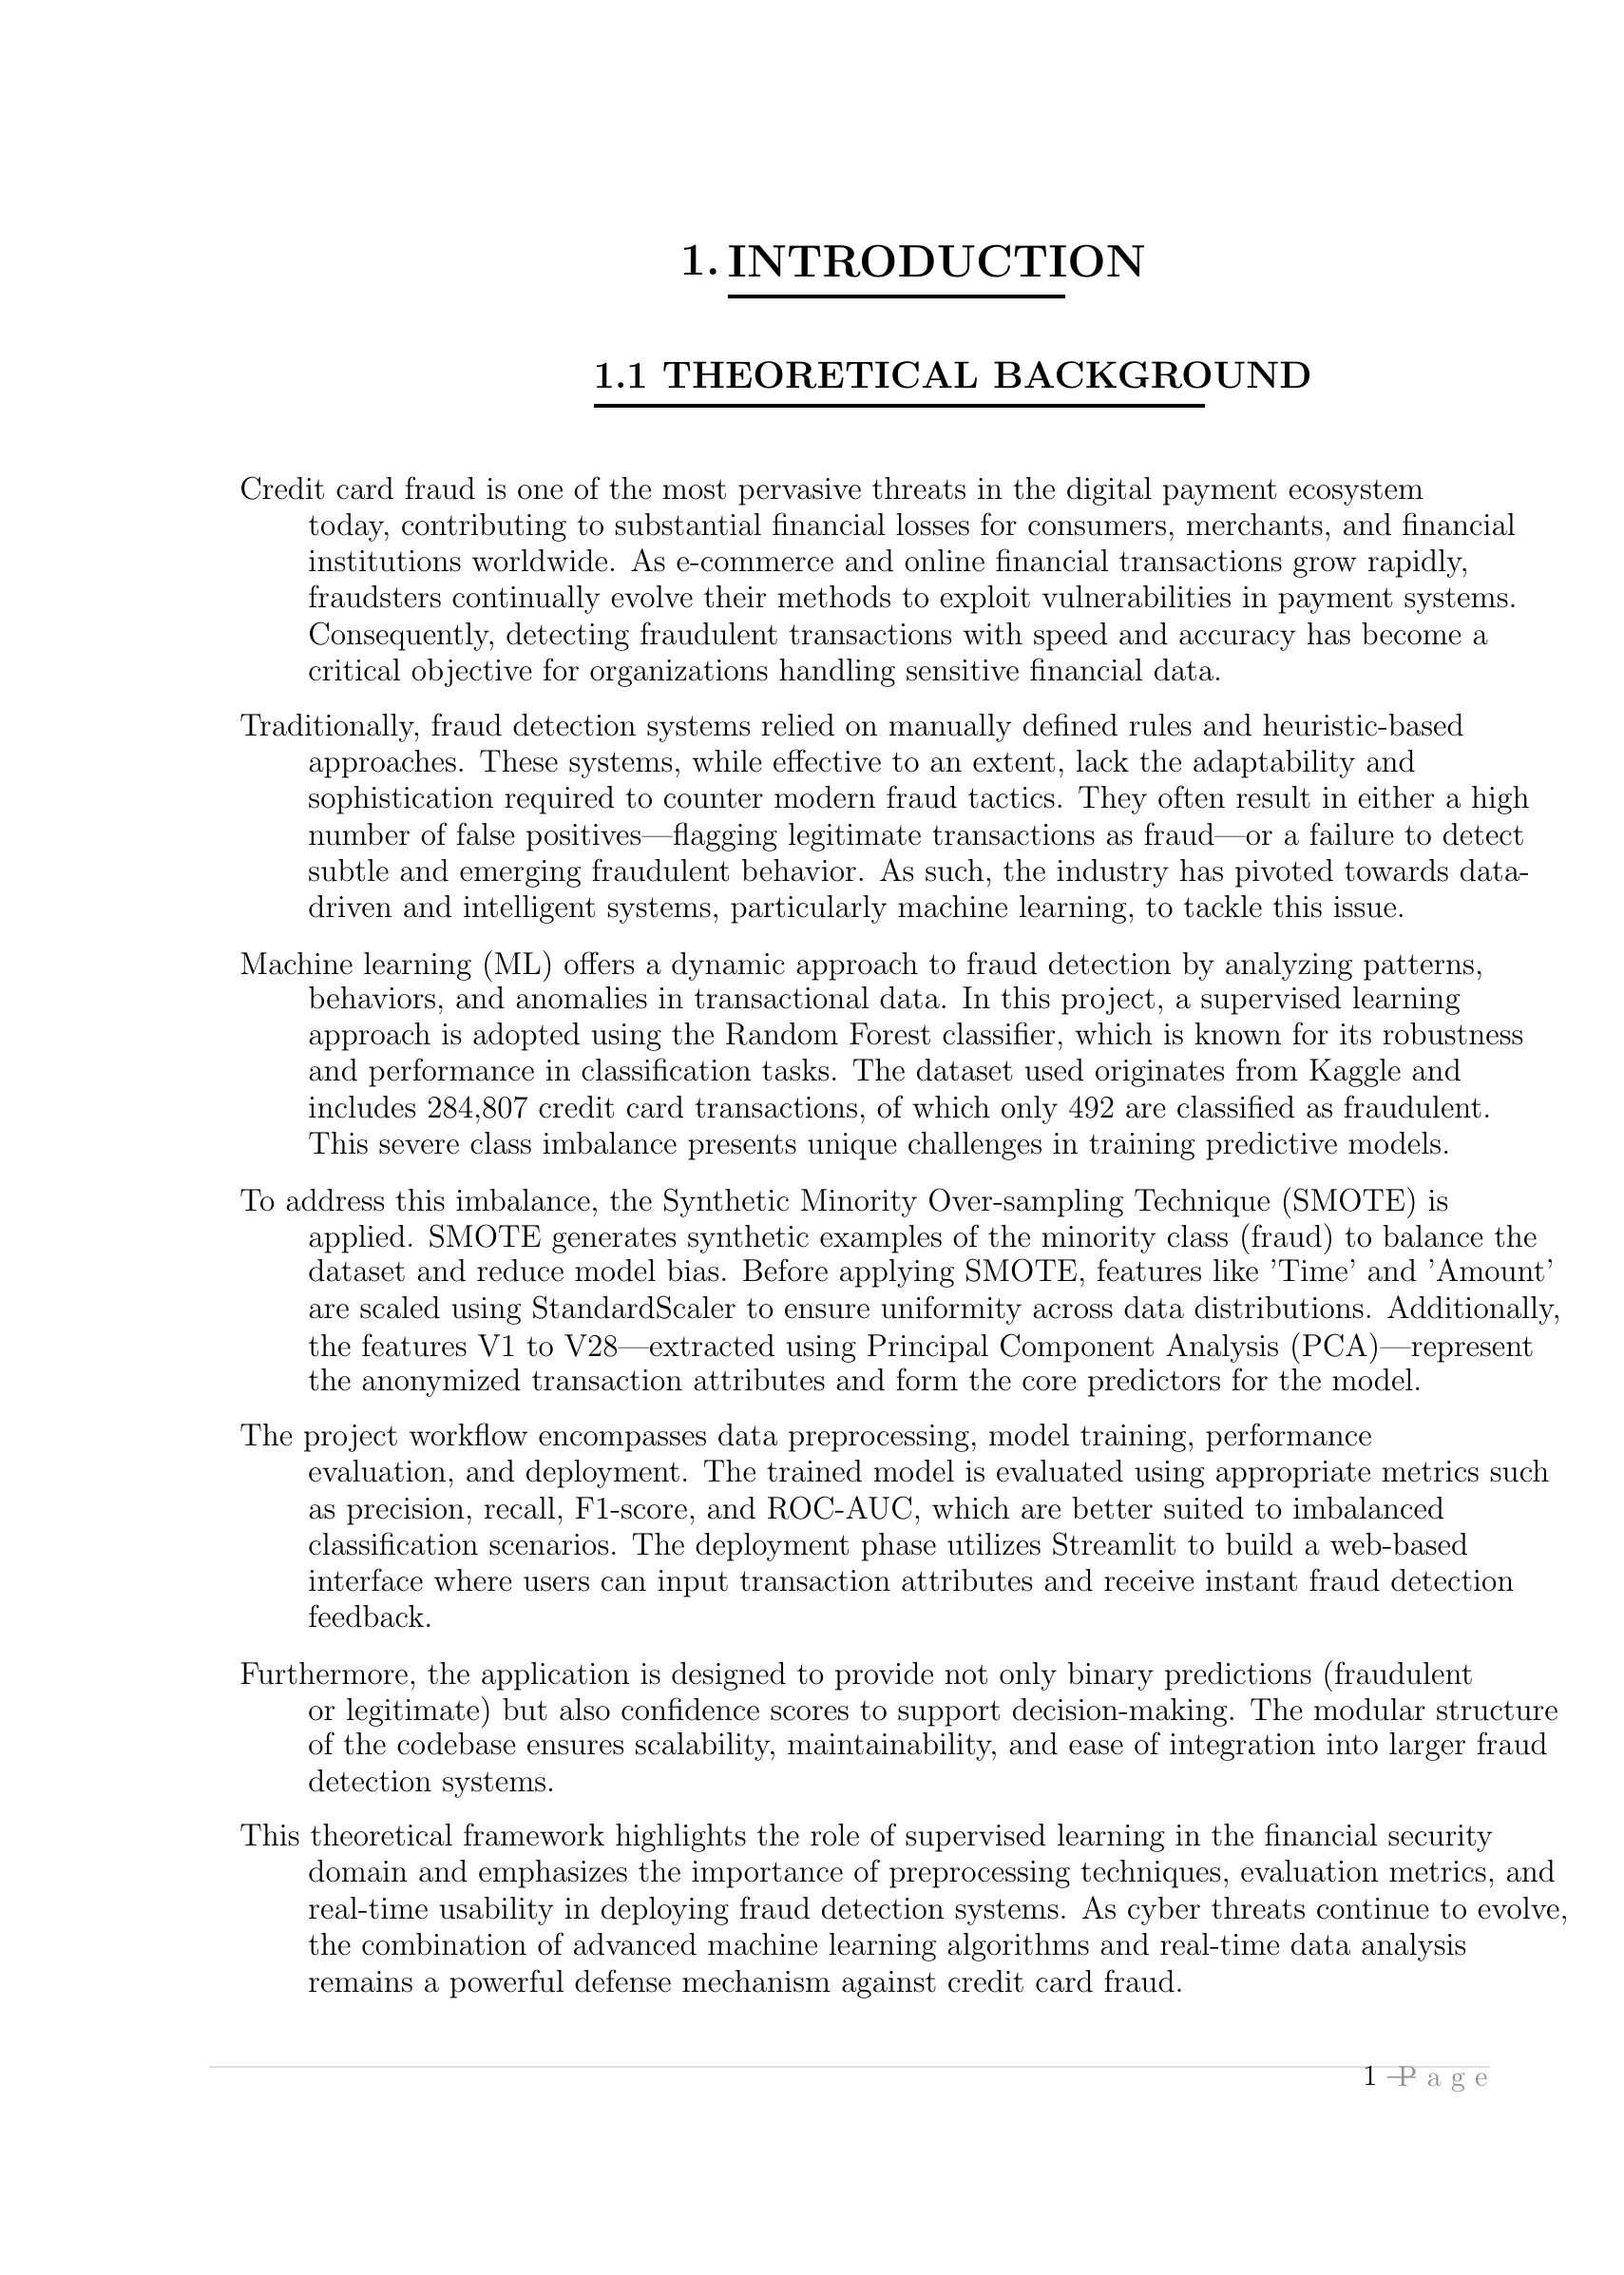
\begin{tikzpicture}[x=1bp,y=-1bp,inner sep=0pt,outer sep=0pt]
  \useasboundingbox (0,0) rectangle (595.20,841.92);
  \fill[fill=pdfcolor9] (69.38,772.78) rectangle (554.40,773.26);
  \fill[fill=black] (265.80,101.78) rectangle (393.77,103.22);
  \fill[fill=black] (214.90,143.09) rectangle (446.36,144.53);
  \node[anchor=north west,inner sep=0pt,outer sep=0pt] at (506.38,772.91) {{\fontsize{11.0bp}{13.2bp}\selectfont 1 | }};
  \node[anchor=north west,inner sep=0pt,outer sep=0pt] at (519.58,772.91) {{\fontsize{11.0bp}{13.2bp}\selectfont \textcolor{pdfcolor1}{P a g e}}};
  \node[anchor=north west,inner sep=0pt,outer sep=0pt] at (550.14,772.91) {{\fontsize{11.0bp}{13.2bp}\selectfont   }};
  \node[anchor=north west,inner sep=0pt,outer sep=0pt] at (247.78,83.31) {{\fontsize{16.1bp}{19.3bp}\selectfont \textbf{1.}}};
  \node[anchor=north west,inner sep=0pt,outer sep=0pt] at (259.80,82.89) {\textsf{{\fontsize{16.1bp}{19.3bp}\selectfont \textbf{ }}}};
  \node[anchor=north west,inner sep=0pt,outer sep=0pt] at (265.80,83.31) {{\fontsize{16.1bp}{19.3bp}\selectfont \textbf{INTRODUCTION }}};
  \node[anchor=north west,inner sep=0pt,outer sep=0pt] at (214.90,127.12) {{\fontsize{13.9bp}{16.7bp}\selectfont \textbf{1.1 THEORETICAL BACKGROUND }}};
  \node[anchor=north west,inner sep=0pt,outer sep=0pt] at (80.90,170.77) {{\fontsize{12.0bp}{14.4bp}\selectfont          Credit card fraud is one of the most pervasive threats in the digital payment ecosystem }};
  \node[anchor=north west,inner sep=0pt,outer sep=0pt] at (106.85,184.45) {{\fontsize{12.0bp}{14.4bp}\selectfont today, contributing to substantial financial losses for consumers, merchants, and financial }};
  \node[anchor=north west,inner sep=0pt,outer sep=0pt] at (106.85,198.37) {{\fontsize{12.0bp}{14.4bp}\selectfont institutions worldwide. As e-commerce and online financial transactions grow rapidly, }};
  \node[anchor=north west,inner sep=0pt,outer sep=0pt] at (106.85,212.07) {{\fontsize{12.0bp}{14.4bp}\selectfont fraudsters continually evolve their methods to exploit vulnerabilities in payment systems. }};
  \node[anchor=north west,inner sep=0pt,outer sep=0pt] at (106.85,225.99) {{\fontsize{12.0bp}{14.4bp}\selectfont Consequently, detecting fraudulent transactions with speed and accuracy has become a }};
  \node[anchor=north west,inner sep=0pt,outer sep=0pt] at (106.85,239.67) {{\fontsize{12.0bp}{14.4bp}\selectfont critical objective for organizations handling sensitive financial data. }};
  \node[anchor=north west,inner sep=0pt,outer sep=0pt] at (80.90,260.55) {{\fontsize{12.0bp}{14.4bp}\selectfont          Traditionally, fraud detection systems relied on manually defined rules and heuristic-based }};
  \node[anchor=north west,inner sep=0pt,outer sep=0pt] at (106.85,274.23) {{\fontsize{12.0bp}{14.4bp}\selectfont approaches. These systems, while effective to an extent, lack the adaptability and }};
  \node[anchor=north west,inner sep=0pt,outer sep=0pt] at (106.85,287.94) {{\fontsize{12.0bp}{14.4bp}\selectfont sophistication required to counter modern fraud tactics. They often result in either a high }};
  \node[anchor=north west,inner sep=0pt,outer sep=0pt] at (106.85,301.86) {{\fontsize{12.0bp}{14.4bp}\selectfont number of false positives---flagging legitimate transactions as fraud---or a failure to detect }};
  \node[anchor=north west,inner sep=0pt,outer sep=0pt] at (106.85,315.54) {{\fontsize{12.0bp}{14.4bp}\selectfont subtle and emerging fraudulent behavior. As such, the industry has pivoted towards data-}};
  \node[anchor=north west,inner sep=0pt,outer sep=0pt] at (106.85,329.46) {{\fontsize{12.0bp}{14.4bp}\selectfont driven and intelligent systems, particularly machine learning, to tackle this issue. }};
  \node[anchor=north west,inner sep=0pt,outer sep=0pt] at (80.90,350.10) {{\fontsize{12.0bp}{14.4bp}\selectfont          Machine learning (ML) offers a dynamic approach to fraud detection by analyzing patterns, }};
  \node[anchor=north west,inner sep=0pt,outer sep=0pt] at (106.85,363.78) {{\fontsize{12.0bp}{14.4bp}\selectfont behaviors, and anomalies in transactional data. In this project, a supervised learning }};
  \node[anchor=north west,inner sep=0pt,outer sep=0pt] at (106.85,377.72) {{\fontsize{12.0bp}{14.4bp}\selectfont approach is adopted using the Random Forest classifier, which is known for its robustness }};
  \node[anchor=north west,inner sep=0pt,outer sep=0pt] at (106.85,391.40) {{\fontsize{12.0bp}{14.4bp}\selectfont and performance in classification tasks. The dataset used originates from Kaggle and }};
  \node[anchor=north west,inner sep=0pt,outer sep=0pt] at (106.85,405.32) {{\fontsize{12.0bp}{14.4bp}\selectfont includes 284,807 credit card transactions, of which only 492 are classified as fraudulent. }};
  \node[anchor=north west,inner sep=0pt,outer sep=0pt] at (106.85,419.00) {{\fontsize{12.0bp}{14.4bp}\selectfont This severe class imbalance presents unique challenges in training predictive models. }};
  \node[anchor=north west,inner sep=0pt,outer sep=0pt] at (80.90,439.88) {{\fontsize{12.0bp}{14.4bp}\selectfont          To address this imbalance, the Synthetic Minority Over-sampling Technique (SMOTE) is }};
  \node[anchor=north west,inner sep=0pt,outer sep=0pt] at (106.85,453.56) {{\fontsize{12.0bp}{14.4bp}\selectfont applied. SMOTE generates synthetic examples of the minority class (fraud) to balance the }};
  \node[anchor=north west,inner sep=0pt,outer sep=0pt] at (106.85,467.26) {{\fontsize{12.0bp}{14.4bp}\selectfont dataset and reduce model bias. Before applying SMOTE, features like 'Time' and 'Amount' }};
  \node[anchor=north west,inner sep=0pt,outer sep=0pt] at (106.85,481.18) {{\fontsize{12.0bp}{14.4bp}\selectfont are scaled using StandardScaler to ensure uniformity across data distributions. Additionally, }};
  \node[anchor=north west,inner sep=0pt,outer sep=0pt] at (106.85,494.86) {{\fontsize{12.0bp}{14.4bp}\selectfont the features V1 to V28---extracted using Principal Component Analysis (PCA)---represent }};
  \node[anchor=north west,inner sep=0pt,outer sep=0pt] at (106.85,508.78) {{\fontsize{12.0bp}{14.4bp}\selectfont the anonymized transaction attributes and form the core predictors for the model. }};
  \node[anchor=north west,inner sep=0pt,outer sep=0pt] at (80.90,529.42) {{\fontsize{12.0bp}{14.4bp}\selectfont          The project workflow encompasses data preprocessing, model training, performance }};
  \node[anchor=north west,inner sep=0pt,outer sep=0pt] at (106.85,543.10) {{\fontsize{12.0bp}{14.4bp}\selectfont evaluation, and deployment. The trained model is evaluated using appropriate metrics such }};
  \node[anchor=north west,inner sep=0pt,outer sep=0pt] at (106.85,557.05) {{\fontsize{12.0bp}{14.4bp}\selectfont as precision, recall, F1-score, and ROC-AUC, which are better suited to imbalanced }};
  \node[anchor=north west,inner sep=0pt,outer sep=0pt] at (106.85,570.73) {{\fontsize{12.0bp}{14.4bp}\selectfont classification scenarios. The deployment phase utilizes Streamlit to build a web-based }};
  \node[anchor=north west,inner sep=0pt,outer sep=0pt] at (106.85,584.65) {{\fontsize{12.0bp}{14.4bp}\selectfont interface where users can input transaction attributes and receive instant fraud detection }};
  \node[anchor=north west,inner sep=0pt,outer sep=0pt] at (106.85,598.33) {{\fontsize{12.0bp}{14.4bp}\selectfont feedback. }};
  \node[anchor=north west,inner sep=0pt,outer sep=0pt] at (80.90,619.21) {{\fontsize{12.0bp}{14.4bp}\selectfont          Furthermore, the application is designed to provide not only binary predictions (fraudulent }};
  \node[anchor=north west,inner sep=0pt,outer sep=0pt] at (106.85,632.91) {{\fontsize{12.0bp}{14.4bp}\selectfont or legitimate) but also confidence scores to support decision-making. The modular structure }};
  \node[anchor=north west,inner sep=0pt,outer sep=0pt] at (106.85,646.59) {{\fontsize{12.0bp}{14.4bp}\selectfont of the codebase ensures scalability, maintainability, and ease of integration into larger fraud }};
  \node[anchor=north west,inner sep=0pt,outer sep=0pt] at (106.85,660.51) {{\fontsize{12.0bp}{14.4bp}\selectfont detection systems. }};
  \node[anchor=north west,inner sep=0pt,outer sep=0pt] at (80.90,681.15) {{\fontsize{12.0bp}{14.4bp}\selectfont         This theoretical framework highlights the role of supervised learning in the financial security }};
  \node[anchor=north west,inner sep=0pt,outer sep=0pt] at (106.85,694.83) {{\fontsize{12.0bp}{14.4bp}\selectfont domain and emphasizes the importance of preprocessing techniques, evaluation metrics, and }};
  \node[anchor=north west,inner sep=0pt,outer sep=0pt] at (106.85,708.75) {{\fontsize{12.0bp}{14.4bp}\selectfont real-time usability in deploying fraud detection systems. As cyber threats continue to evolve, }};
  \node[anchor=north west,inner sep=0pt,outer sep=0pt] at (106.85,722.46) {{\fontsize{12.0bp}{14.4bp}\selectfont the combination of advanced machine learning algorithms and real-time data analysis }};
  \node[anchor=north west,inner sep=0pt,outer sep=0pt] at (106.85,736.38) {{\fontsize{12.0bp}{14.4bp}\selectfont remains a powerful defense mechanism against credit card fraud. }};
\end{tikzpicture}
\newpage
\noindent
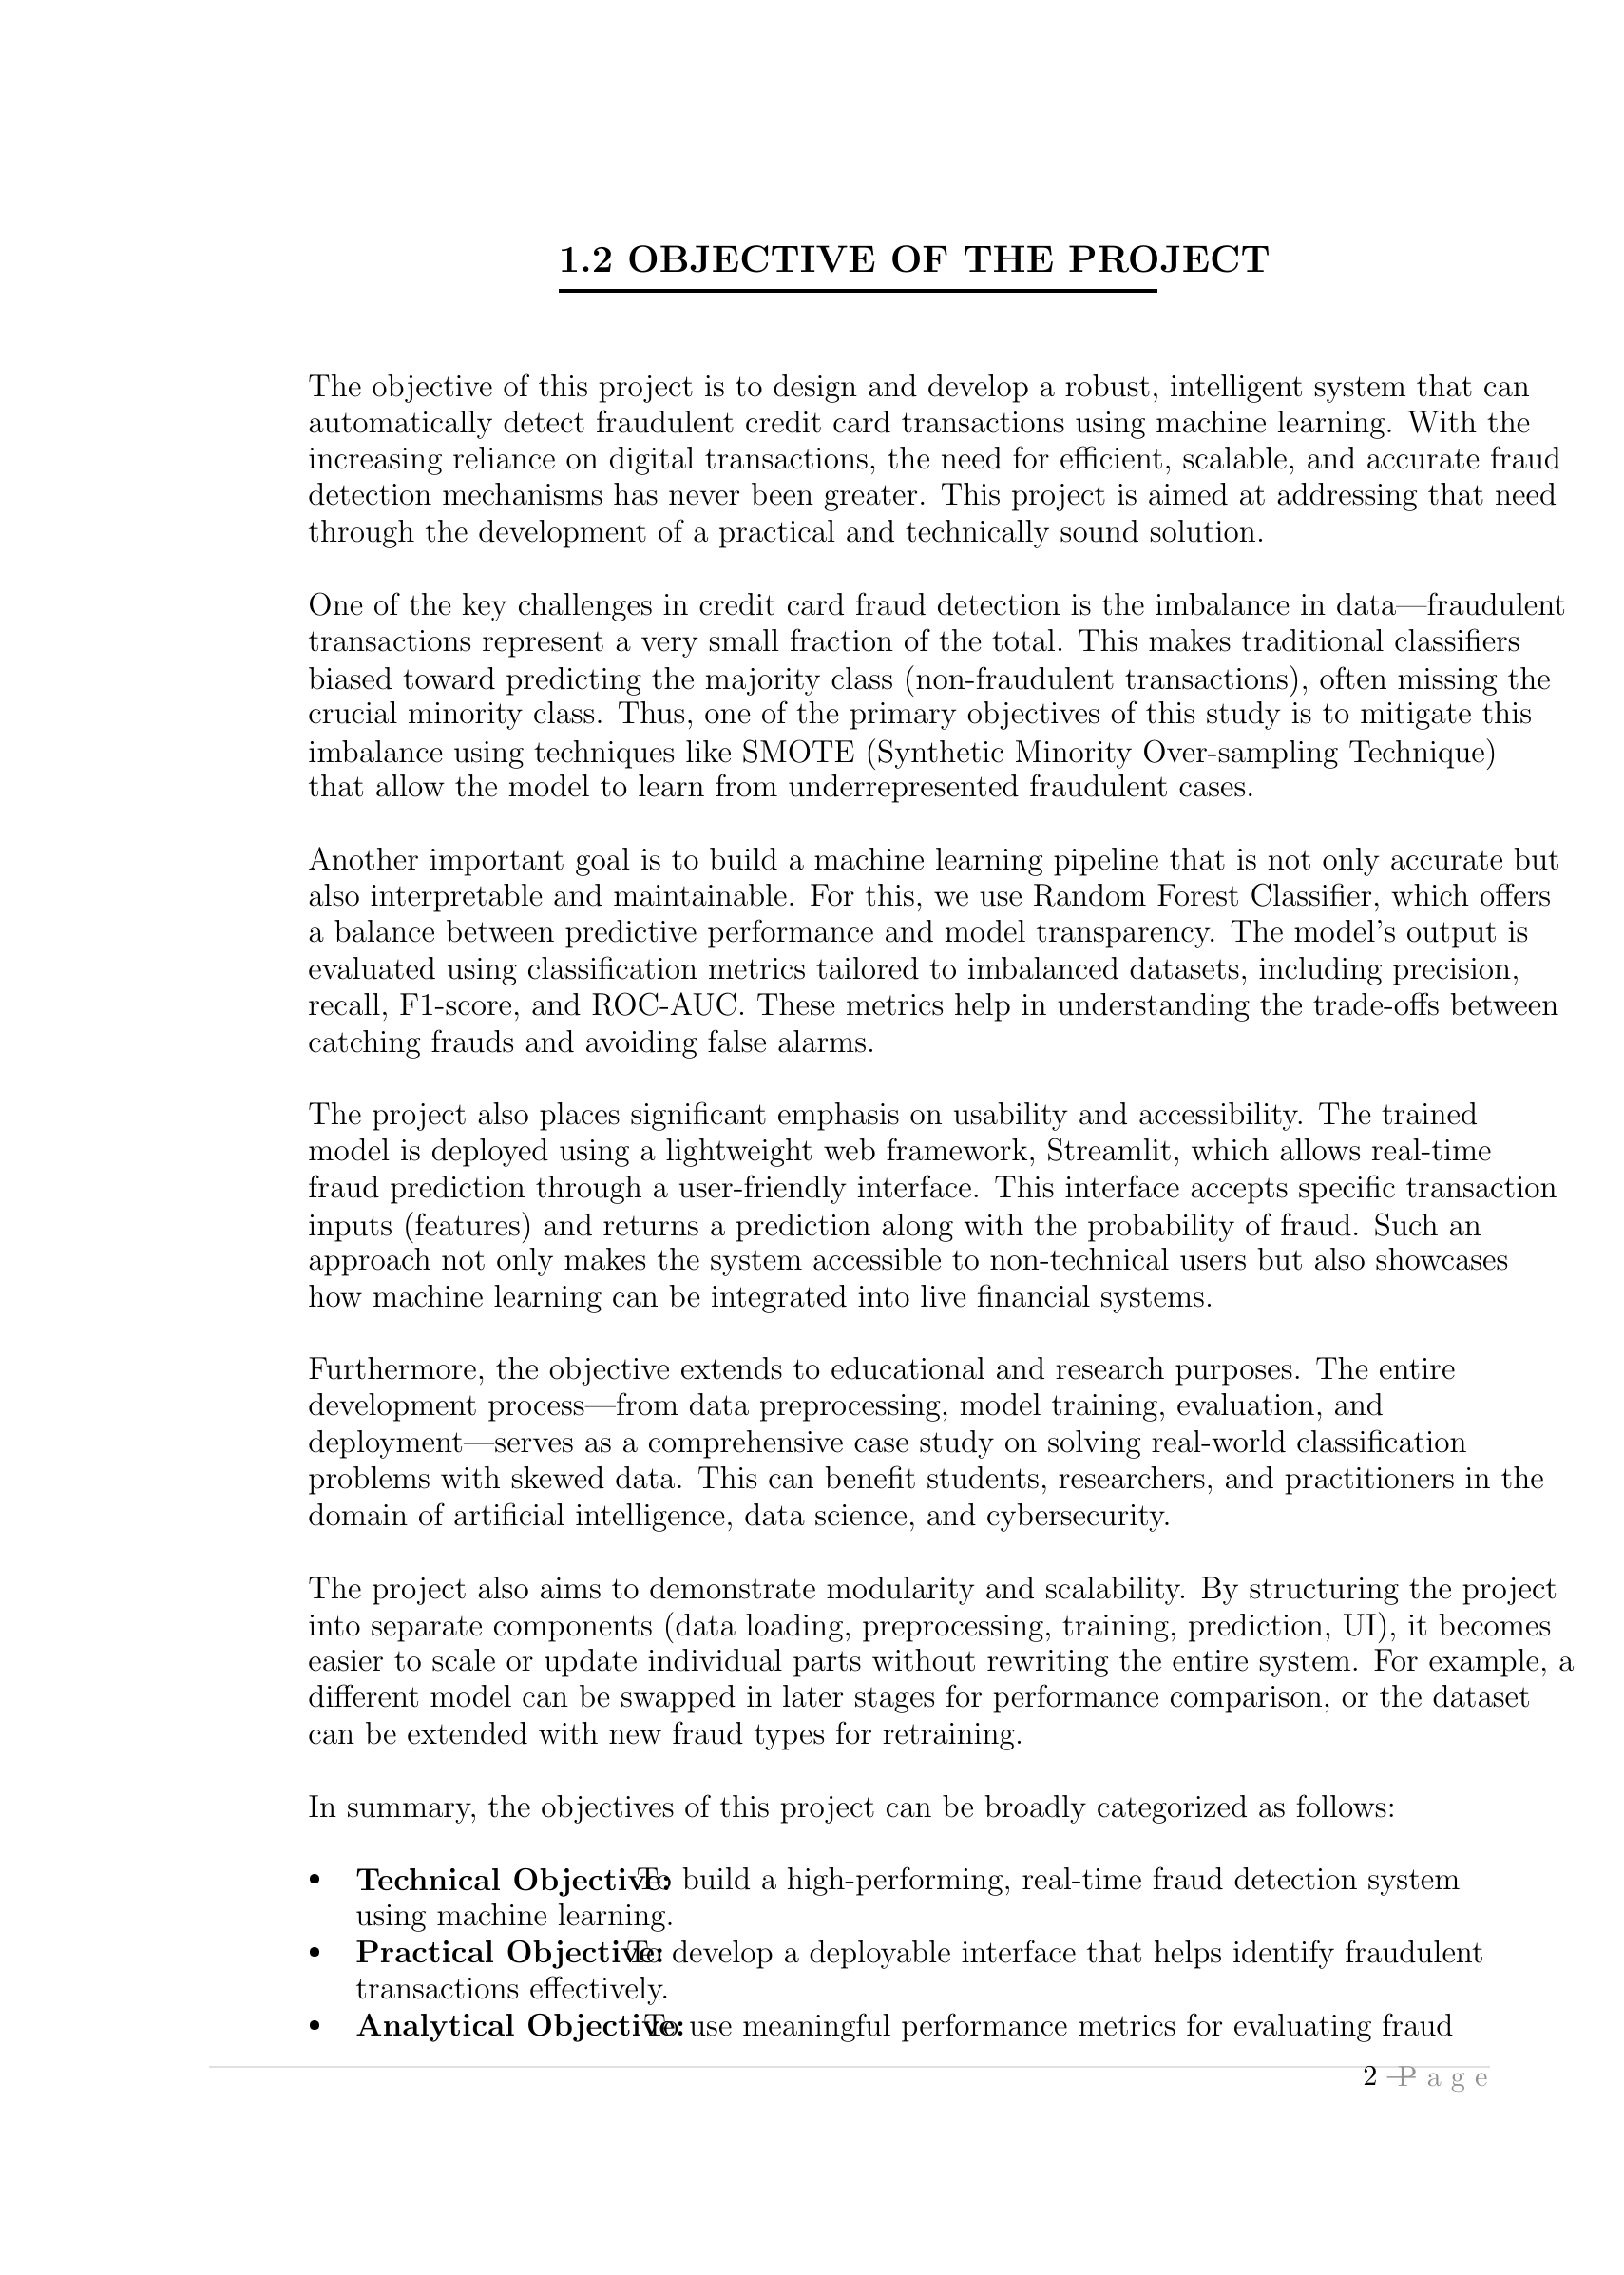
\begin{tikzpicture}[x=1bp,y=-1bp,inner sep=0pt,outer sep=0pt]
  \useasboundingbox (0,0) rectangle (595.20,841.92);
  \fill[fill=pdfcolor9] (69.38,772.78) rectangle (554.40,773.26);
  \fill[fill=black] (201.70,99.38) rectangle (428.60,100.82);
  \node[anchor=north west,inner sep=0pt,outer sep=0pt] at (506.38,772.91) {{\fontsize{11.0bp}{13.2bp}\selectfont 2 | }};
  \node[anchor=north west,inner sep=0pt,outer sep=0pt] at (519.58,772.91) {{\fontsize{11.0bp}{13.2bp}\selectfont \textcolor{pdfcolor1}{P a g e}}};
  \node[anchor=north west,inner sep=0pt,outer sep=0pt] at (550.14,772.91) {{\fontsize{11.0bp}{13.2bp}\selectfont   }};
  \node[anchor=north west,inner sep=0pt,outer sep=0pt] at (201.70,83.41) {{\fontsize{13.9bp}{16.7bp}\selectfont \textbf{1.2 OBJECTIVE OF THE PROJECT }}};
  \node[anchor=north west,inner sep=0pt,outer sep=0pt] at (106.85,99.49) {{\fontsize{13.9bp}{16.7bp}\selectfont \textbf{ }}};
  \node[anchor=north west,inner sep=0pt,outer sep=0pt] at (106.85,115.84) {{\fontsize{13.9bp}{16.7bp}\selectfont \textbf{ }}};
  \node[anchor=north west,inner sep=0pt,outer sep=0pt] at (106.85,131.89) {{\fontsize{12.0bp}{14.4bp}\selectfont The objective of this project is to design and develop a robust, intelligent system that can }};
  \node[anchor=north west,inner sep=0pt,outer sep=0pt] at (106.85,145.57) {{\fontsize{12.0bp}{14.4bp}\selectfont automatically detect fraudulent credit card transactions using machine learning. With the }};
  \node[anchor=north west,inner sep=0pt,outer sep=0pt] at (106.85,159.49) {{\fontsize{12.0bp}{14.4bp}\selectfont increasing reliance on digital transactions, the need for efficient, scalable, and accurate fraud }};
  \node[anchor=north west,inner sep=0pt,outer sep=0pt] at (106.85,173.17) {{\fontsize{12.0bp}{14.4bp}\selectfont detection mechanisms has never been greater. This project is aimed at addressing that need }};
  \node[anchor=north west,inner sep=0pt,outer sep=0pt] at (106.85,187.09) {{\fontsize{12.0bp}{14.4bp}\selectfont through the development of a practical and technically sound solution. }};
  \node[anchor=north west,inner sep=0pt,outer sep=0pt] at (106.85,200.79) {{\fontsize{12.0bp}{14.4bp}\selectfont  }};
  \node[anchor=north west,inner sep=0pt,outer sep=0pt] at (106.85,214.71) {{\fontsize{12.0bp}{14.4bp}\selectfont One of the key challenges in credit card fraud detection is the imbalance in data---fraudulent }};
  \node[anchor=north west,inner sep=0pt,outer sep=0pt] at (106.85,228.39) {{\fontsize{12.0bp}{14.4bp}\selectfont transactions represent a very small fraction of the total. This makes traditional classifiers }};
  \node[anchor=north west,inner sep=0pt,outer sep=0pt] at (106.85,242.31) {{\fontsize{12.0bp}{14.4bp}\selectfont biased toward predicting the majority class (non-fraudulent transactions), often missing the }};
  \node[anchor=north west,inner sep=0pt,outer sep=0pt] at (106.85,255.99) {{\fontsize{12.0bp}{14.4bp}\selectfont crucial minority class. Thus, one of the primary objectives of this study is to mitigate this }};
  \node[anchor=north west,inner sep=0pt,outer sep=0pt] at (106.85,269.91) {{\fontsize{12.0bp}{14.4bp}\selectfont imbalance using techniques like SMOTE (Synthetic Minority Over-sampling Technique) }};
  \node[anchor=north west,inner sep=0pt,outer sep=0pt] at (106.85,283.59) {{\fontsize{12.0bp}{14.4bp}\selectfont that allow the model to learn from underrepresented fraudulent cases. }};
  \node[anchor=north west,inner sep=0pt,outer sep=0pt] at (106.85,297.54) {{\fontsize{12.0bp}{14.4bp}\selectfont  }};
  \node[anchor=north west,inner sep=0pt,outer sep=0pt] at (106.85,311.22) {{\fontsize{12.0bp}{14.4bp}\selectfont Another important goal is to build a machine learning pipeline that is not only accurate but }};
  \node[anchor=north west,inner sep=0pt,outer sep=0pt] at (106.85,325.14) {{\fontsize{12.0bp}{14.4bp}\selectfont also interpretable and maintainable. For this, we use Random Forest Classifier, which offers }};
  \node[anchor=north west,inner sep=0pt,outer sep=0pt] at (106.85,338.82) {{\fontsize{12.0bp}{14.4bp}\selectfont a balance between predictive performance and model transparency. The model's output is }};
  \node[anchor=north west,inner sep=0pt,outer sep=0pt] at (106.85,352.74) {{\fontsize{12.0bp}{14.4bp}\selectfont evaluated using classification metrics tailored to imbalanced datasets, including precision, }};
  \node[anchor=north west,inner sep=0pt,outer sep=0pt] at (106.85,366.42) {{\fontsize{12.0bp}{14.4bp}\selectfont recall, F1-score, and ROC-AUC. These metrics help in understanding the trade-offs between }};
  \node[anchor=north west,inner sep=0pt,outer sep=0pt] at (106.85,380.36) {{\fontsize{12.0bp}{14.4bp}\selectfont catching frauds and avoiding false alarms. }};
  \node[anchor=north west,inner sep=0pt,outer sep=0pt] at (106.85,394.04) {{\fontsize{12.0bp}{14.4bp}\selectfont  }};
  \node[anchor=north west,inner sep=0pt,outer sep=0pt] at (106.85,407.96) {{\fontsize{12.0bp}{14.4bp}\selectfont The project also places significant emphasis on usability and accessibility. The trained }};
  \node[anchor=north west,inner sep=0pt,outer sep=0pt] at (106.85,421.64) {{\fontsize{12.0bp}{14.4bp}\selectfont model is deployed using a lightweight web framework, Streamlit, which allows real-time }};
  \node[anchor=north west,inner sep=0pt,outer sep=0pt] at (106.85,435.56) {{\fontsize{12.0bp}{14.4bp}\selectfont fraud prediction through a user-friendly interface. This interface accepts specific transaction }};
  \node[anchor=north west,inner sep=0pt,outer sep=0pt] at (106.85,449.24) {{\fontsize{12.0bp}{14.4bp}\selectfont inputs (features) and returns a prediction along with the probability of fraud. Such an }};
  \node[anchor=north west,inner sep=0pt,outer sep=0pt] at (106.85,462.94) {{\fontsize{12.0bp}{14.4bp}\selectfont approach not only makes the system accessible to non-technical users but also showcases }};
  \node[anchor=north west,inner sep=0pt,outer sep=0pt] at (106.85,476.86) {{\fontsize{12.0bp}{14.4bp}\selectfont how machine learning can be integrated into live financial systems. }};
  \node[anchor=north west,inner sep=0pt,outer sep=0pt] at (106.85,490.54) {{\fontsize{12.0bp}{14.4bp}\selectfont  }};
  \node[anchor=north west,inner sep=0pt,outer sep=0pt] at (106.85,504.46) {{\fontsize{12.0bp}{14.4bp}\selectfont Furthermore, the objective extends to educational and research purposes. The entire }};
  \node[anchor=north west,inner sep=0pt,outer sep=0pt] at (106.85,518.14) {{\fontsize{12.0bp}{14.4bp}\selectfont development process---from data preprocessing, model training, evaluation, and }};
  \node[anchor=north west,inner sep=0pt,outer sep=0pt] at (106.85,532.06) {{\fontsize{12.0bp}{14.4bp}\selectfont deployment---serves as a comprehensive case study on solving real-world classification }};
  \node[anchor=north west,inner sep=0pt,outer sep=0pt] at (106.85,545.77) {{\fontsize{12.0bp}{14.4bp}\selectfont problems with skewed data. This can benefit students, researchers, and practitioners in the }};
  \node[anchor=north west,inner sep=0pt,outer sep=0pt] at (106.85,559.69) {{\fontsize{12.0bp}{14.4bp}\selectfont domain of artificial intelligence, data science, and cybersecurity. }};
  \node[anchor=north west,inner sep=0pt,outer sep=0pt] at (106.85,573.37) {{\fontsize{12.0bp}{14.4bp}\selectfont  }};
  \node[anchor=north west,inner sep=0pt,outer sep=0pt] at (106.85,587.29) {{\fontsize{12.0bp}{14.4bp}\selectfont The project also aims to demonstrate modularity and scalability. By structuring the project }};
  \node[anchor=north west,inner sep=0pt,outer sep=0pt] at (106.85,600.97) {{\fontsize{12.0bp}{14.4bp}\selectfont into separate components (data loading, preprocessing, training, prediction, UI), it becomes }};
  \node[anchor=north west,inner sep=0pt,outer sep=0pt] at (106.85,614.89) {{\fontsize{12.0bp}{14.4bp}\selectfont easier to scale or update individual parts without rewriting the entire system. For example, a }};
  \node[anchor=north west,inner sep=0pt,outer sep=0pt] at (106.85,628.57) {{\fontsize{12.0bp}{14.4bp}\selectfont different model can be swapped in later stages for performance comparison, or the dataset }};
  \node[anchor=north west,inner sep=0pt,outer sep=0pt] at (106.85,642.51) {{\fontsize{12.0bp}{14.4bp}\selectfont can be extended with new fraud types for retraining. }};
  \node[anchor=north west,inner sep=0pt,outer sep=0pt] at (106.85,656.19) {{\fontsize{12.0bp}{14.4bp}\selectfont  }};
  \node[anchor=north west,inner sep=0pt,outer sep=0pt] at (106.85,670.11) {{\fontsize{12.0bp}{14.4bp}\selectfont In summary, the objectives of this project can be broadly categorized as follows: }};
  \node[anchor=north west,inner sep=0pt,outer sep=0pt] at (106.85,683.79) {{\fontsize{12.0bp}{14.4bp}\selectfont  }};
  \node[anchor=north west,inner sep=0pt,outer sep=0pt] at (106.85,700.22) {{\fontsize{10.1bp}{12.1bp}\selectfont •}};
  \node[anchor=north west,inner sep=0pt,outer sep=0pt] at (111.41,699.51) {\textsf{{\fontsize{10.1bp}{12.1bp}\selectfont  }}};
  \node[anchor=north west,inner sep=0pt,outer sep=0pt] at (124.85,697.82) {{\fontsize{12.0bp}{14.4bp}\selectfont \textbf{Technical Objective:}}};
  \node[anchor=north west,inner sep=0pt,outer sep=0pt] at (231.22,697.71) {{\fontsize{12.0bp}{14.4bp}\selectfont  To build a high-performing, real-time fraud detection system }};
  \node[anchor=north west,inner sep=0pt,outer sep=0pt] at (124.85,711.39) {{\fontsize{12.0bp}{14.4bp}\selectfont using machine learning. }};
  \node[anchor=north west,inner sep=0pt,outer sep=0pt] at (106.85,727.85) {{\fontsize{10.1bp}{12.1bp}\selectfont •}};
  \node[anchor=north west,inner sep=0pt,outer sep=0pt] at (111.41,727.14) {\textsf{{\fontsize{10.1bp}{12.1bp}\selectfont  }}};
  \node[anchor=north west,inner sep=0pt,outer sep=0pt] at (124.85,725.45) {{\fontsize{12.0bp}{14.4bp}\selectfont \textbf{Practical Objective:}}};
  \node[anchor=north west,inner sep=0pt,outer sep=0pt] at (227.38,725.34) {{\fontsize{12.0bp}{14.4bp}\selectfont  To develop a deployable interface that helps identify fraudulent }};
  \node[anchor=north west,inner sep=0pt,outer sep=0pt] at (124.85,739.02) {{\fontsize{12.0bp}{14.4bp}\selectfont transactions effectively. }};
  \node[anchor=north west,inner sep=0pt,outer sep=0pt] at (106.85,755.44) {{\fontsize{10.1bp}{12.1bp}\selectfont •}};
  \node[anchor=north west,inner sep=0pt,outer sep=0pt] at (111.41,754.74) {\textsf{{\fontsize{10.1bp}{12.1bp}\selectfont  }}};
  \node[anchor=north west,inner sep=0pt,outer sep=0pt] at (124.85,753.05) {{\fontsize{12.0bp}{14.4bp}\selectfont \textbf{Analytical Objective:}}};
  \node[anchor=north west,inner sep=0pt,outer sep=0pt] at (233.86,752.94) {{\fontsize{12.0bp}{14.4bp}\selectfont  To use meaningful performance metrics for evaluating fraud }};
\end{tikzpicture}
\newpage
\noindent

\begin{tikzpicture}[x=1bp,y=-1bp,inner sep=0pt,outer sep=0pt]
  \useasboundingbox (0,0) rectangle (595.20,841.92);
  \fill[fill=pdfcolor9] (69.38,772.78) rectangle (554.40,773.26);
  \fill[fill=black] (222.10,292.63) rectangle (396.65,294.07);
  \node[anchor=north west,inner sep=0pt,outer sep=0pt] at (506.38,772.91) {{\fontsize{11.0bp}{13.2bp}\selectfont 3 | }};
  \node[anchor=north west,inner sep=0pt,outer sep=0pt] at (519.58,772.91) {{\fontsize{11.0bp}{13.2bp}\selectfont \textcolor{pdfcolor1}{P a g e}}};
  \node[anchor=north west,inner sep=0pt,outer sep=0pt] at (550.14,772.91) {{\fontsize{11.0bp}{13.2bp}\selectfont   }};
  \node[anchor=north west,inner sep=0pt,outer sep=0pt] at (124.85,83.38) {{\fontsize{12.0bp}{14.4bp}\selectfont detection accuracy. }};
  \node[anchor=north west,inner sep=0pt,outer sep=0pt] at (106.85,99.81) {{\fontsize{10.1bp}{12.1bp}\selectfont •}};
  \node[anchor=north west,inner sep=0pt,outer sep=0pt] at (111.41,99.10) {\textsf{{\fontsize{10.1bp}{12.1bp}\selectfont  }}};
  \node[anchor=north west,inner sep=0pt,outer sep=0pt] at (124.85,97.41) {{\fontsize{12.0bp}{14.4bp}\selectfont \textbf{Educational Objective:}}};
  \node[anchor=north west,inner sep=0pt,outer sep=0pt] at (243.22,97.30) {{\fontsize{12.0bp}{14.4bp}\selectfont  To serve as a learning resource for end-to-end ML pipeline }};
  \node[anchor=north west,inner sep=0pt,outer sep=0pt] at (124.85,110.98) {{\fontsize{12.0bp}{14.4bp}\selectfont development. }};
  \node[anchor=north west,inner sep=0pt,outer sep=0pt] at (106.85,127.44) {{\fontsize{10.1bp}{12.1bp}\selectfont •}};
  \node[anchor=north west,inner sep=0pt,outer sep=0pt] at (111.41,126.73) {\textsf{{\fontsize{10.1bp}{12.1bp}\selectfont  }}};
  \node[anchor=north west,inner sep=0pt,outer sep=0pt] at (124.85,125.04) {{\fontsize{12.0bp}{14.4bp}\selectfont \textbf{Scalability Objective:}}};
  \node[anchor=north west,inner sep=0pt,outer sep=0pt] at (235.30,124.93) {{\fontsize{12.0bp}{14.4bp}\selectfont  To ensure modular code that can be reused and extended in real-}};
  \node[anchor=north west,inner sep=0pt,outer sep=0pt] at (124.85,138.61) {{\fontsize{12.0bp}{14.4bp}\selectfont world applications. }};
  \node[anchor=north west,inner sep=0pt,outer sep=0pt] at (124.85,152.53) {{\fontsize{12.0bp}{14.4bp}\selectfont  }};
  \node[anchor=north west,inner sep=0pt,outer sep=0pt] at (106.85,166.21) {{\fontsize{12.0bp}{14.4bp}\selectfont Achieving these objectives not only contributes to mitigating the impact of credit card fraud }};
  \node[anchor=north west,inner sep=0pt,outer sep=0pt] at (106.85,180.13) {{\fontsize{12.0bp}{14.4bp}\selectfont but also provides a reusable framework for similar classification problems in other domains }};
  \node[anchor=north west,inner sep=0pt,outer sep=0pt] at (106.85,193.81) {{\fontsize{12.0bp}{14.4bp}\selectfont such as insurance fraud, loan defaults, and cyber threat detection }};
  \node[anchor=north west,inner sep=0pt,outer sep=0pt] at (106.85,207.75) {{\fontsize{12.0bp}{14.4bp}\selectfont  }};
  \node[anchor=north west,inner sep=0pt,outer sep=0pt] at (106.85,221.46) {{\fontsize{13.9bp}{16.7bp}\selectfont \textbf{ }}};
  \node[anchor=north west,inner sep=0pt,outer sep=0pt] at (214.90,276.66) {{\fontsize{13.9bp}{16.7bp}\selectfont \textbf{  1.3 SCOPE OF THE STUDY }}};
  \node[anchor=north west,inner sep=0pt,outer sep=0pt] at (70.82,334.02) {{\fontsize{12.0bp}{14.4bp}\selectfont The scope of this project extends across multiple phases of the machine learning lifecycle, including }};
  \node[anchor=north west,inner sep=0pt,outer sep=0pt] at (70.82,349.86) {{\fontsize{12.0bp}{14.4bp}\selectfont data acquisition, preprocessing, model training, performance evaluation, and real-time deployment. }};
  \node[anchor=north west,inner sep=0pt,outer sep=0pt] at (70.82,365.70) {{\fontsize{12.0bp}{14.4bp}\selectfont The study aims to address both the technical and practical aspects of credit card fraud detection by }};
  \node[anchor=north west,inner sep=0pt,outer sep=0pt] at (70.82,381.56) {{\fontsize{12.0bp}{14.4bp}\selectfont implementing a robust and modular machine learning system. }};
  \node[anchor=north west,inner sep=0pt,outer sep=0pt] at (70.82,407.48) {{\fontsize{12.0bp}{14.4bp}\selectfont This project utilizes a publicly available, real-world credit card transaction dataset that includes }};
  \node[anchor=north west,inner sep=0pt,outer sep=0pt] at (70.82,423.32) {{\fontsize{12.0bp}{14.4bp}\selectfont anonymized features derived using Principal Component Analysis (PCA). The dataset offers a }};
  \node[anchor=north west,inner sep=0pt,outer sep=0pt] at (70.82,439.16) {{\fontsize{12.0bp}{14.4bp}\selectfont realistic setting with severe class imbalance, as fraudulent transactions account for only a tiny }};
  \node[anchor=north west,inner sep=0pt,outer sep=0pt] at (70.82,455.00) {{\fontsize{12.0bp}{14.4bp}\selectfont fraction of the total. This makes it a suitable testbed for evaluating machine learning algorithms }};
  \node[anchor=north west,inner sep=0pt,outer sep=0pt] at (70.82,470.86) {{\fontsize{12.0bp}{14.4bp}\selectfont under challenging conditions. }};
  \node[anchor=north west,inner sep=0pt,outer sep=0pt] at (70.82,496.78) {{\fontsize{12.0bp}{14.4bp}\selectfont The implementation focuses on the supervised classification paradigm using the Random Forest }};
  \node[anchor=north west,inner sep=0pt,outer sep=0pt] at (70.82,512.62) {{\fontsize{12.0bp}{14.4bp}\selectfont algorithm, chosen for its interpretability, performance, and resistance to overfitting. The model is }};
  \node[anchor=north west,inner sep=0pt,outer sep=0pt] at (70.82,528.46) {{\fontsize{12.0bp}{14.4bp}\selectfont trained on preprocessed data, where features such as 'Time' and 'Amount' are standardized and class }};
  \node[anchor=north west,inner sep=0pt,outer sep=0pt] at (70.82,544.33) {{\fontsize{12.0bp}{14.4bp}\selectfont imbalance is mitigated using the Synthetic Minority Over-sampling Technique (SMOTE). These }};
  \node[anchor=north west,inner sep=0pt,outer sep=0pt] at (70.82,560.17) {{\fontsize{12.0bp}{14.4bp}\selectfont preprocessing steps are crucial for ensuring the model learns meaningful patterns from the minority }};
  \node[anchor=north west,inner sep=0pt,outer sep=0pt] at (70.82,576.25) {{\fontsize{12.0bp}{14.4bp}\selectfont class. }};
  \node[anchor=north west,inner sep=0pt,outer sep=0pt] at (70.82,601.93) {{\fontsize{12.0bp}{14.4bp}\selectfont The system is also designed to be interactive and accessible. A lightweight user interface is }};
  \node[anchor=north west,inner sep=0pt,outer sep=0pt] at (70.82,617.77) {{\fontsize{12.0bp}{14.4bp}\selectfont developed using Streamlit, allowing real-time fraud detection based on user-input transaction }};
  \node[anchor=north west,inner sep=0pt,outer sep=0pt] at (70.82,633.87) {{\fontsize{12.0bp}{14.4bp}\selectfont features. This UI not only demonstrates the practical applicability of the model but also provides a }};
  \node[anchor=north west,inner sep=0pt,outer sep=0pt] at (70.82,649.71) {{\fontsize{12.0bp}{14.4bp}\selectfont foundation for future integration with real-world payment systems. }};
  \node[anchor=north west,inner sep=0pt,outer sep=0pt] at (70.82,675.39) {{\fontsize{12.0bp}{14.4bp}\selectfont The scope further includes evaluating the model using a comprehensive set of metrics. Metrics such }};
  \node[anchor=north west,inner sep=0pt,outer sep=0pt] at (70.82,691.47) {{\fontsize{12.0bp}{14.4bp}\selectfont as precision, recall, F1-score, and ROC-AUC are used to assess the model's performance, }};
  \node[anchor=north west,inner sep=0pt,outer sep=0pt] at (70.82,707.31) {{\fontsize{12.0bp}{14.4bp}\selectfont particularly its ability to detect frauds without producing excessive false positives. Visualizations }};
  \node[anchor=north west,inner sep=0pt,outer sep=0pt] at (70.82,723.18) {{\fontsize{12.0bp}{14.4bp}\selectfont like confusion matrices and ROC curves help interpret and validate the results. }};
\end{tikzpicture}
\newpage
\noindent
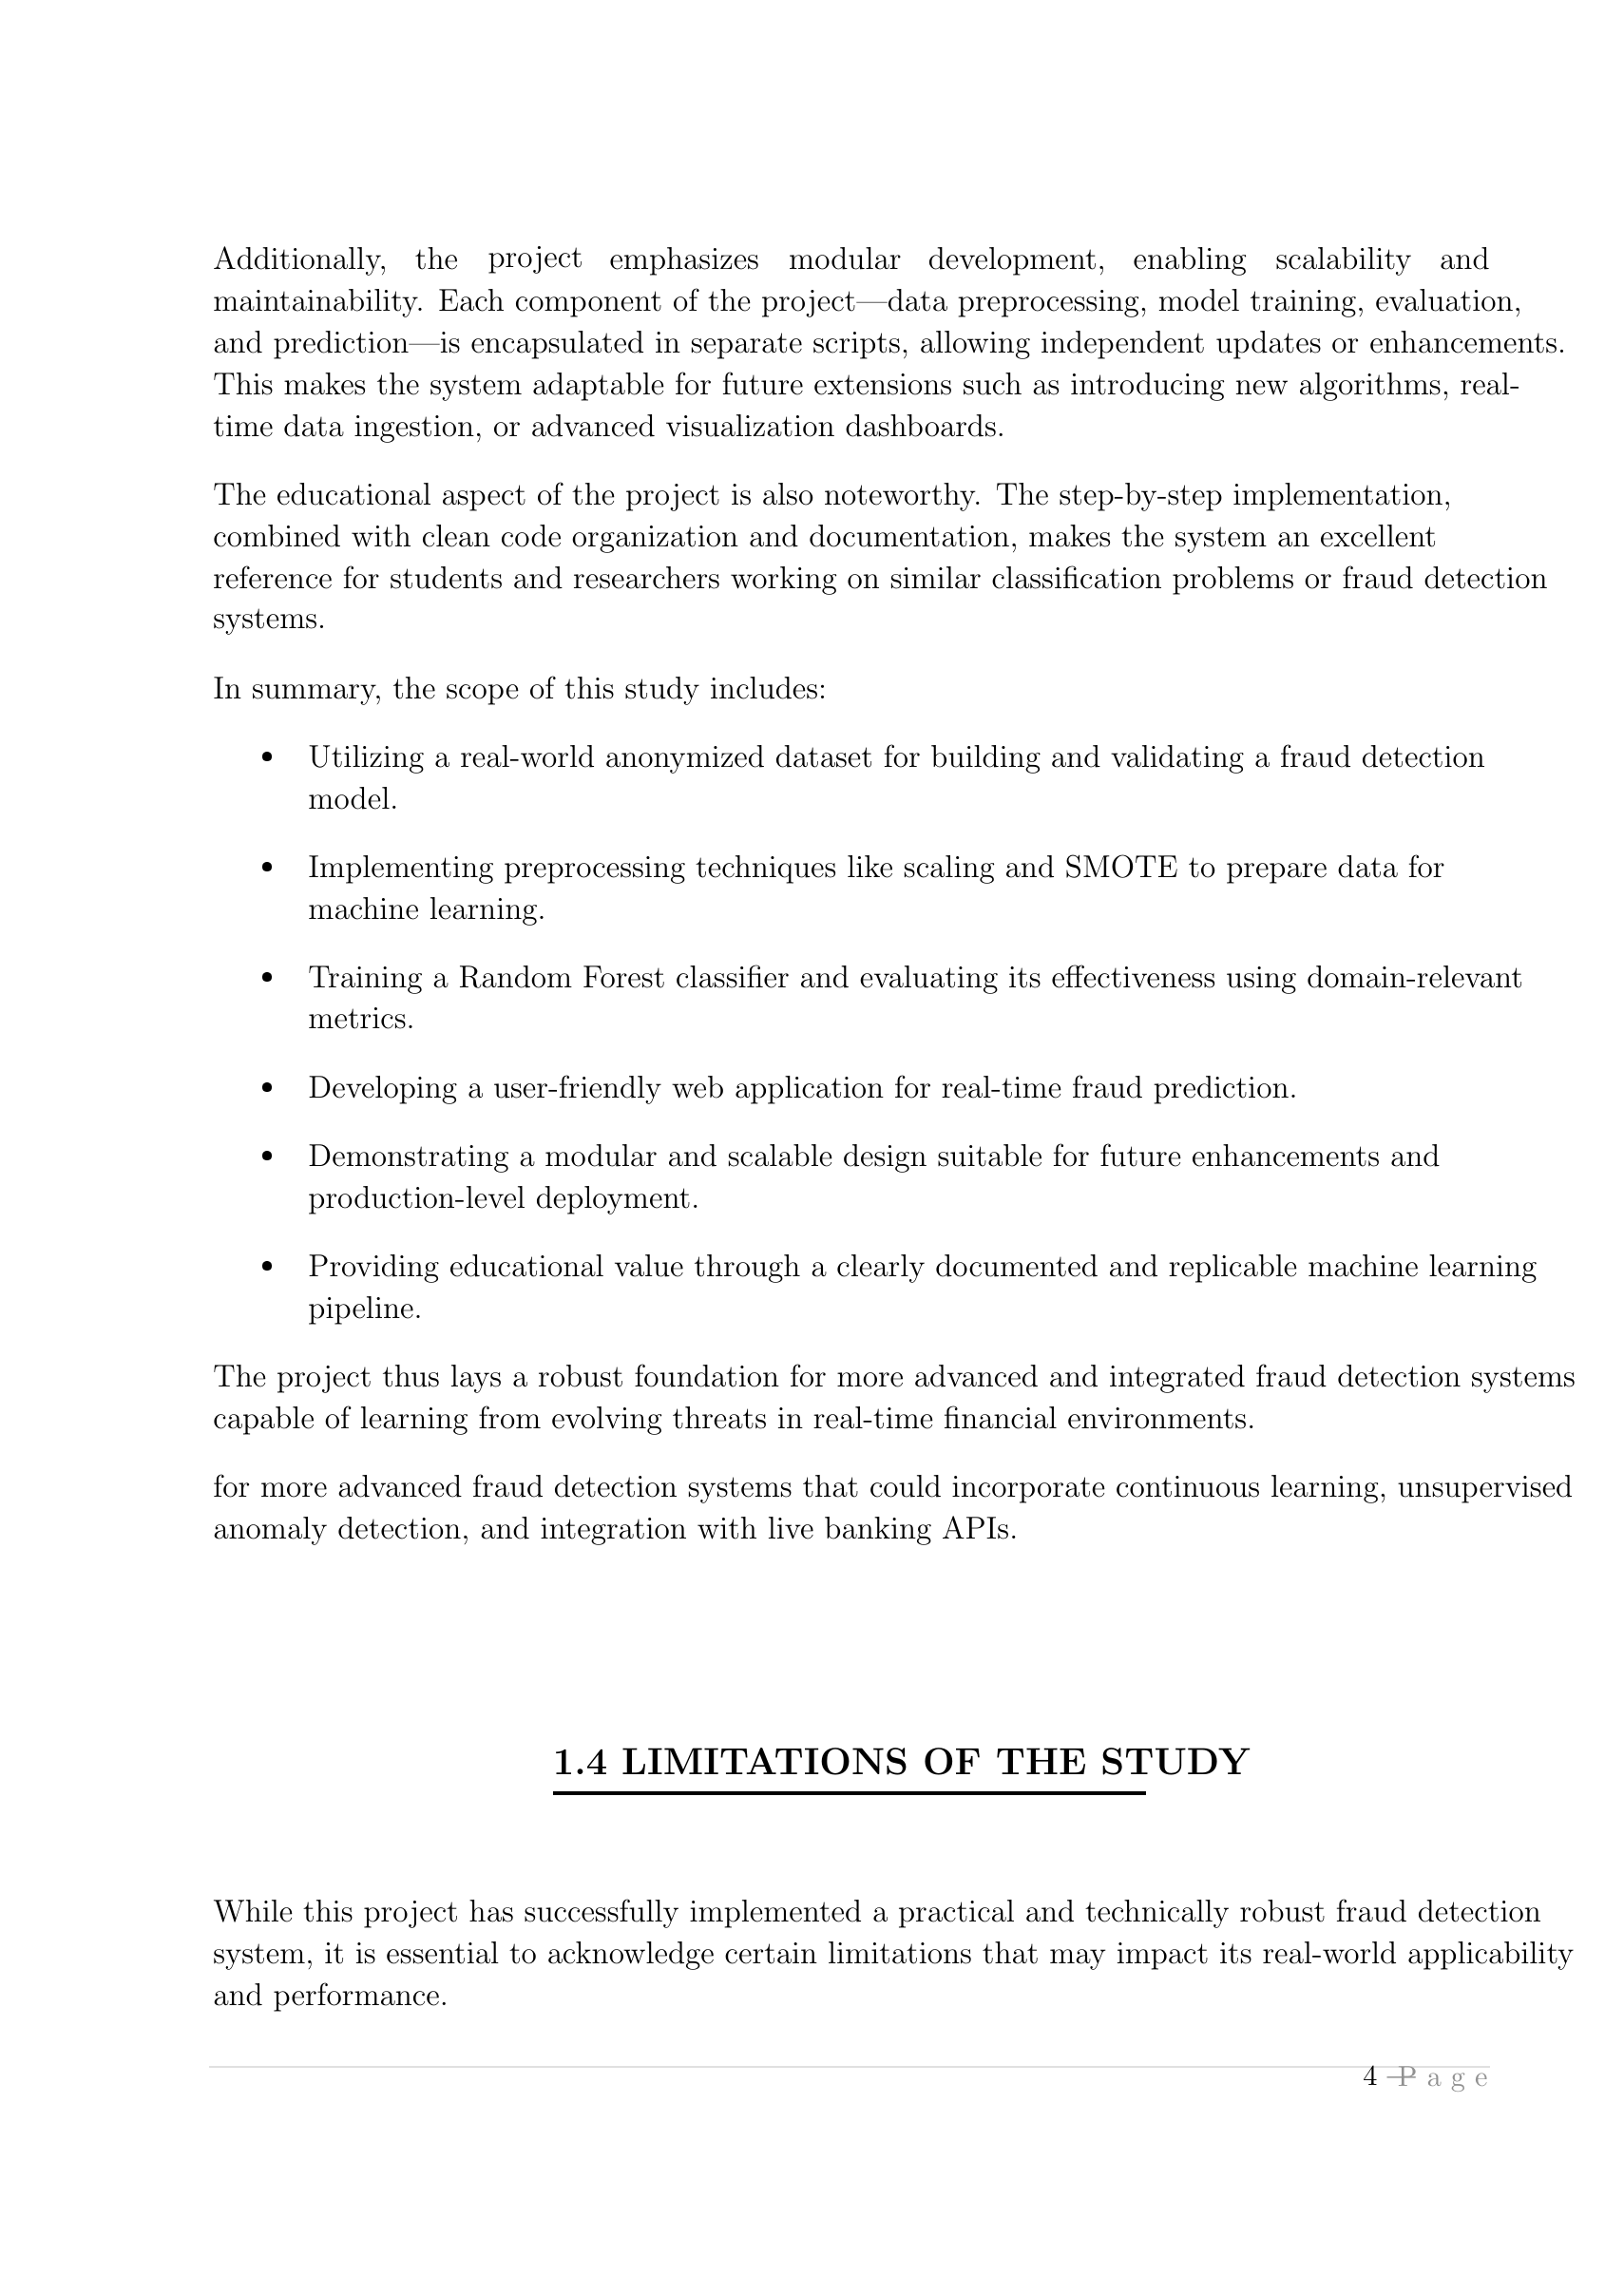
\begin{tikzpicture}[x=1bp,y=-1bp,inner sep=0pt,outer sep=0pt]
  \useasboundingbox (0,0) rectangle (595.20,841.92);
  \fill[fill=pdfcolor9] (69.38,772.78) rectangle (554.40,773.26);
  \fill[fill=black] (199.54,668.59) rectangle (424.04,670.03);
  \node[anchor=north west,inner sep=0pt,outer sep=0pt] at (506.38,772.91) {{\fontsize{11.0bp}{13.2bp}\selectfont 4 | }};
  \node[anchor=north west,inner sep=0pt,outer sep=0pt] at (519.58,772.91) {{\fontsize{11.0bp}{13.2bp}\selectfont \textcolor{pdfcolor1}{P a g e}}};
  \node[anchor=north west,inner sep=0pt,outer sep=0pt] at (550.14,772.91) {{\fontsize{11.0bp}{13.2bp}\selectfont   }};
  \node[anchor=north west,inner sep=0pt,outer sep=0pt] at (70.82,83.62) {{\fontsize{12.0bp}{14.4bp}\selectfont Additionally, }};
  \node[anchor=north west,inner sep=0pt,outer sep=0pt] at (147.35,83.62) {{\fontsize{12.0bp}{14.4bp}\selectfont the }};
  \node[anchor=north west,inner sep=0pt,outer sep=0pt] at (174.94,83.62) {{\fontsize{12.0bp}{14.4bp}\selectfont project }};
  \node[anchor=north west,inner sep=0pt,outer sep=0pt] at (220.99,83.62) {{\fontsize{12.0bp}{14.4bp}\selectfont emphasizes }};
  \node[anchor=north west,inner sep=0pt,outer sep=0pt] at (288.90,83.62) {{\fontsize{12.0bp}{14.4bp}\selectfont modular }};
  \node[anchor=north west,inner sep=0pt,outer sep=0pt] at (341.68,83.62) {{\fontsize{12.0bp}{14.4bp}\selectfont development, }};
  \node[anchor=north west,inner sep=0pt,outer sep=0pt] at (419.41,83.62) {{\fontsize{12.0bp}{14.4bp}\selectfont enabling }};
  \node[anchor=north west,inner sep=0pt,outer sep=0pt] at (473.39,83.62) {{\fontsize{12.0bp}{14.4bp}\selectfont scalability }};
  \node[anchor=north west,inner sep=0pt,outer sep=0pt] at (535.52,83.62) {{\fontsize{12.0bp}{14.4bp}\selectfont and }};
  \node[anchor=north west,inner sep=0pt,outer sep=0pt] at (70.82,99.46) {{\fontsize{12.0bp}{14.4bp}\selectfont maintainability. Each component of the project---data preprocessing, model training, evaluation, }};
  \node[anchor=north west,inner sep=0pt,outer sep=0pt] at (70.82,115.57) {{\fontsize{12.0bp}{14.4bp}\selectfont and prediction---is encapsulated in separate scripts, allowing independent updates or enhancements. }};
  \node[anchor=north west,inner sep=0pt,outer sep=0pt] at (70.82,131.41) {{\fontsize{12.0bp}{14.4bp}\selectfont This makes the system adaptable for future extensions such as introducing new algorithms, real-}};
  \node[anchor=north west,inner sep=0pt,outer sep=0pt] at (70.82,147.25) {{\fontsize{12.0bp}{14.4bp}\selectfont time data ingestion, or advanced visualization dashboards. }};
  \node[anchor=north west,inner sep=0pt,outer sep=0pt] at (70.82,173.17) {{\fontsize{12.0bp}{14.4bp}\selectfont The educational aspect of the project is also noteworthy. The step-by-step implementation, }};
  \node[anchor=north west,inner sep=0pt,outer sep=0pt] at (70.82,189.01) {{\fontsize{12.0bp}{14.4bp}\selectfont combined with clean code organization and documentation, makes the system an excellent }};
  \node[anchor=north west,inner sep=0pt,outer sep=0pt] at (70.82,204.87) {{\fontsize{12.0bp}{14.4bp}\selectfont reference for students and researchers working on similar classification problems or fraud detection }};
  \node[anchor=north west,inner sep=0pt,outer sep=0pt] at (70.82,220.71) {{\fontsize{12.0bp}{14.4bp}\selectfont systems. }};
  \node[anchor=north west,inner sep=0pt,outer sep=0pt] at (70.82,246.63) {{\fontsize{12.0bp}{14.4bp}\selectfont In summary, the scope of this study includes: }};
  \node[anchor=north west,inner sep=0pt,outer sep=0pt] at (88.85,275.06) {{\fontsize{10.1bp}{12.1bp}\selectfont •}};
  \node[anchor=north west,inner sep=0pt,outer sep=0pt] at (93.41,274.35) {\textsf{{\fontsize{10.1bp}{12.1bp}\selectfont  }}};
  \node[anchor=north west,inner sep=0pt,outer sep=0pt] at (106.85,272.55) {{\fontsize{12.0bp}{14.4bp}\selectfont Utilizing a real-world anonymized dataset for building and validating a fraud detection }};
  \node[anchor=north west,inner sep=0pt,outer sep=0pt] at (106.85,288.42) {{\fontsize{12.0bp}{14.4bp}\selectfont model. }};
  \node[anchor=north west,inner sep=0pt,outer sep=0pt] at (88.85,316.61) {{\fontsize{10.1bp}{12.1bp}\selectfont •}};
  \node[anchor=north west,inner sep=0pt,outer sep=0pt] at (93.41,315.90) {\textsf{{\fontsize{10.1bp}{12.1bp}\selectfont  }}};
  \node[anchor=north west,inner sep=0pt,outer sep=0pt] at (106.85,314.10) {{\fontsize{12.0bp}{14.4bp}\selectfont Implementing preprocessing techniques like scaling and SMOTE to prepare data for }};
  \node[anchor=north west,inner sep=0pt,outer sep=0pt] at (106.85,330.18) {{\fontsize{12.0bp}{14.4bp}\selectfont machine learning. }};
  \node[anchor=north west,inner sep=0pt,outer sep=0pt] at (88.85,358.37) {{\fontsize{10.1bp}{12.1bp}\selectfont •}};
  \node[anchor=north west,inner sep=0pt,outer sep=0pt] at (93.41,357.66) {\textsf{{\fontsize{10.1bp}{12.1bp}\selectfont  }}};
  \node[anchor=north west,inner sep=0pt,outer sep=0pt] at (106.85,355.86) {{\fontsize{12.0bp}{14.4bp}\selectfont Training a Random Forest classifier and evaluating its effectiveness using domain-relevant }};
  \node[anchor=north west,inner sep=0pt,outer sep=0pt] at (106.85,371.72) {{\fontsize{12.0bp}{14.4bp}\selectfont metrics. }};
  \node[anchor=north west,inner sep=0pt,outer sep=0pt] at (88.85,400.15) {{\fontsize{10.1bp}{12.1bp}\selectfont •}};
  \node[anchor=north west,inner sep=0pt,outer sep=0pt] at (93.41,399.44) {\textsf{{\fontsize{10.1bp}{12.1bp}\selectfont  }}};
  \node[anchor=north west,inner sep=0pt,outer sep=0pt] at (106.85,397.64) {{\fontsize{12.0bp}{14.4bp}\selectfont Developing a user-friendly web application for real-time fraud prediction. }};
  \node[anchor=north west,inner sep=0pt,outer sep=0pt] at (88.85,426.07) {{\fontsize{10.1bp}{12.1bp}\selectfont •}};
  \node[anchor=north west,inner sep=0pt,outer sep=0pt] at (93.41,425.36) {\textsf{{\fontsize{10.1bp}{12.1bp}\selectfont  }}};
  \node[anchor=north west,inner sep=0pt,outer sep=0pt] at (106.85,423.56) {{\fontsize{12.0bp}{14.4bp}\selectfont Demonstrating a modular and scalable design suitable for future enhancements and }};
  \node[anchor=north west,inner sep=0pt,outer sep=0pt] at (106.85,439.40) {{\fontsize{12.0bp}{14.4bp}\selectfont production-level deployment. }};
  \node[anchor=north west,inner sep=0pt,outer sep=0pt] at (88.85,467.85) {{\fontsize{10.1bp}{12.1bp}\selectfont •}};
  \node[anchor=north west,inner sep=0pt,outer sep=0pt] at (93.41,467.14) {\textsf{{\fontsize{10.1bp}{12.1bp}\selectfont  }}};
  \node[anchor=north west,inner sep=0pt,outer sep=0pt] at (106.85,465.34) {{\fontsize{12.0bp}{14.4bp}\selectfont Providing educational value through a clearly documented and replicable machine learning }};
  \node[anchor=north west,inner sep=0pt,outer sep=0pt] at (106.85,481.18) {{\fontsize{12.0bp}{14.4bp}\selectfont pipeline. }};
  \node[anchor=north west,inner sep=0pt,outer sep=0pt] at (70.82,507.10) {{\fontsize{12.0bp}{14.4bp}\selectfont The project thus lays a robust foundation for more advanced and integrated fraud detection systems }};
  \node[anchor=north west,inner sep=0pt,outer sep=0pt] at (70.82,522.94) {{\fontsize{12.0bp}{14.4bp}\selectfont capable of learning from evolving threats in real-time financial environments. }};
  \node[anchor=north west,inner sep=0pt,outer sep=0pt] at (70.82,548.89) {{\fontsize{12.0bp}{14.4bp}\selectfont for more advanced fraud detection systems that could incorporate continuous learning, unsupervised }};
  \node[anchor=north west,inner sep=0pt,outer sep=0pt] at (70.82,564.73) {{\fontsize{12.0bp}{14.4bp}\selectfont anomaly detection, and integration with live banking APIs. }};
  \node[anchor=north west,inner sep=0pt,outer sep=0pt] at (199.54,652.62) {{\fontsize{13.9bp}{16.7bp}\selectfont \textbf{1.4 LIMITATIONS OF THE STUDY }}};
  \node[anchor=north west,inner sep=0pt,outer sep=0pt] at (70.82,709.95) {{\fontsize{12.0bp}{14.4bp}\selectfont While this project has successfully implemented a practical and technically robust fraud detection }};
  \node[anchor=north west,inner sep=0pt,outer sep=0pt] at (70.82,725.82) {{\fontsize{12.0bp}{14.4bp}\selectfont system, it is essential to acknowledge certain limitations that may impact its real-world applicability }};
  \node[anchor=north west,inner sep=0pt,outer sep=0pt] at (70.82,741.66) {{\fontsize{12.0bp}{14.4bp}\selectfont and performance. }};
\end{tikzpicture}
\newpage
\noindent
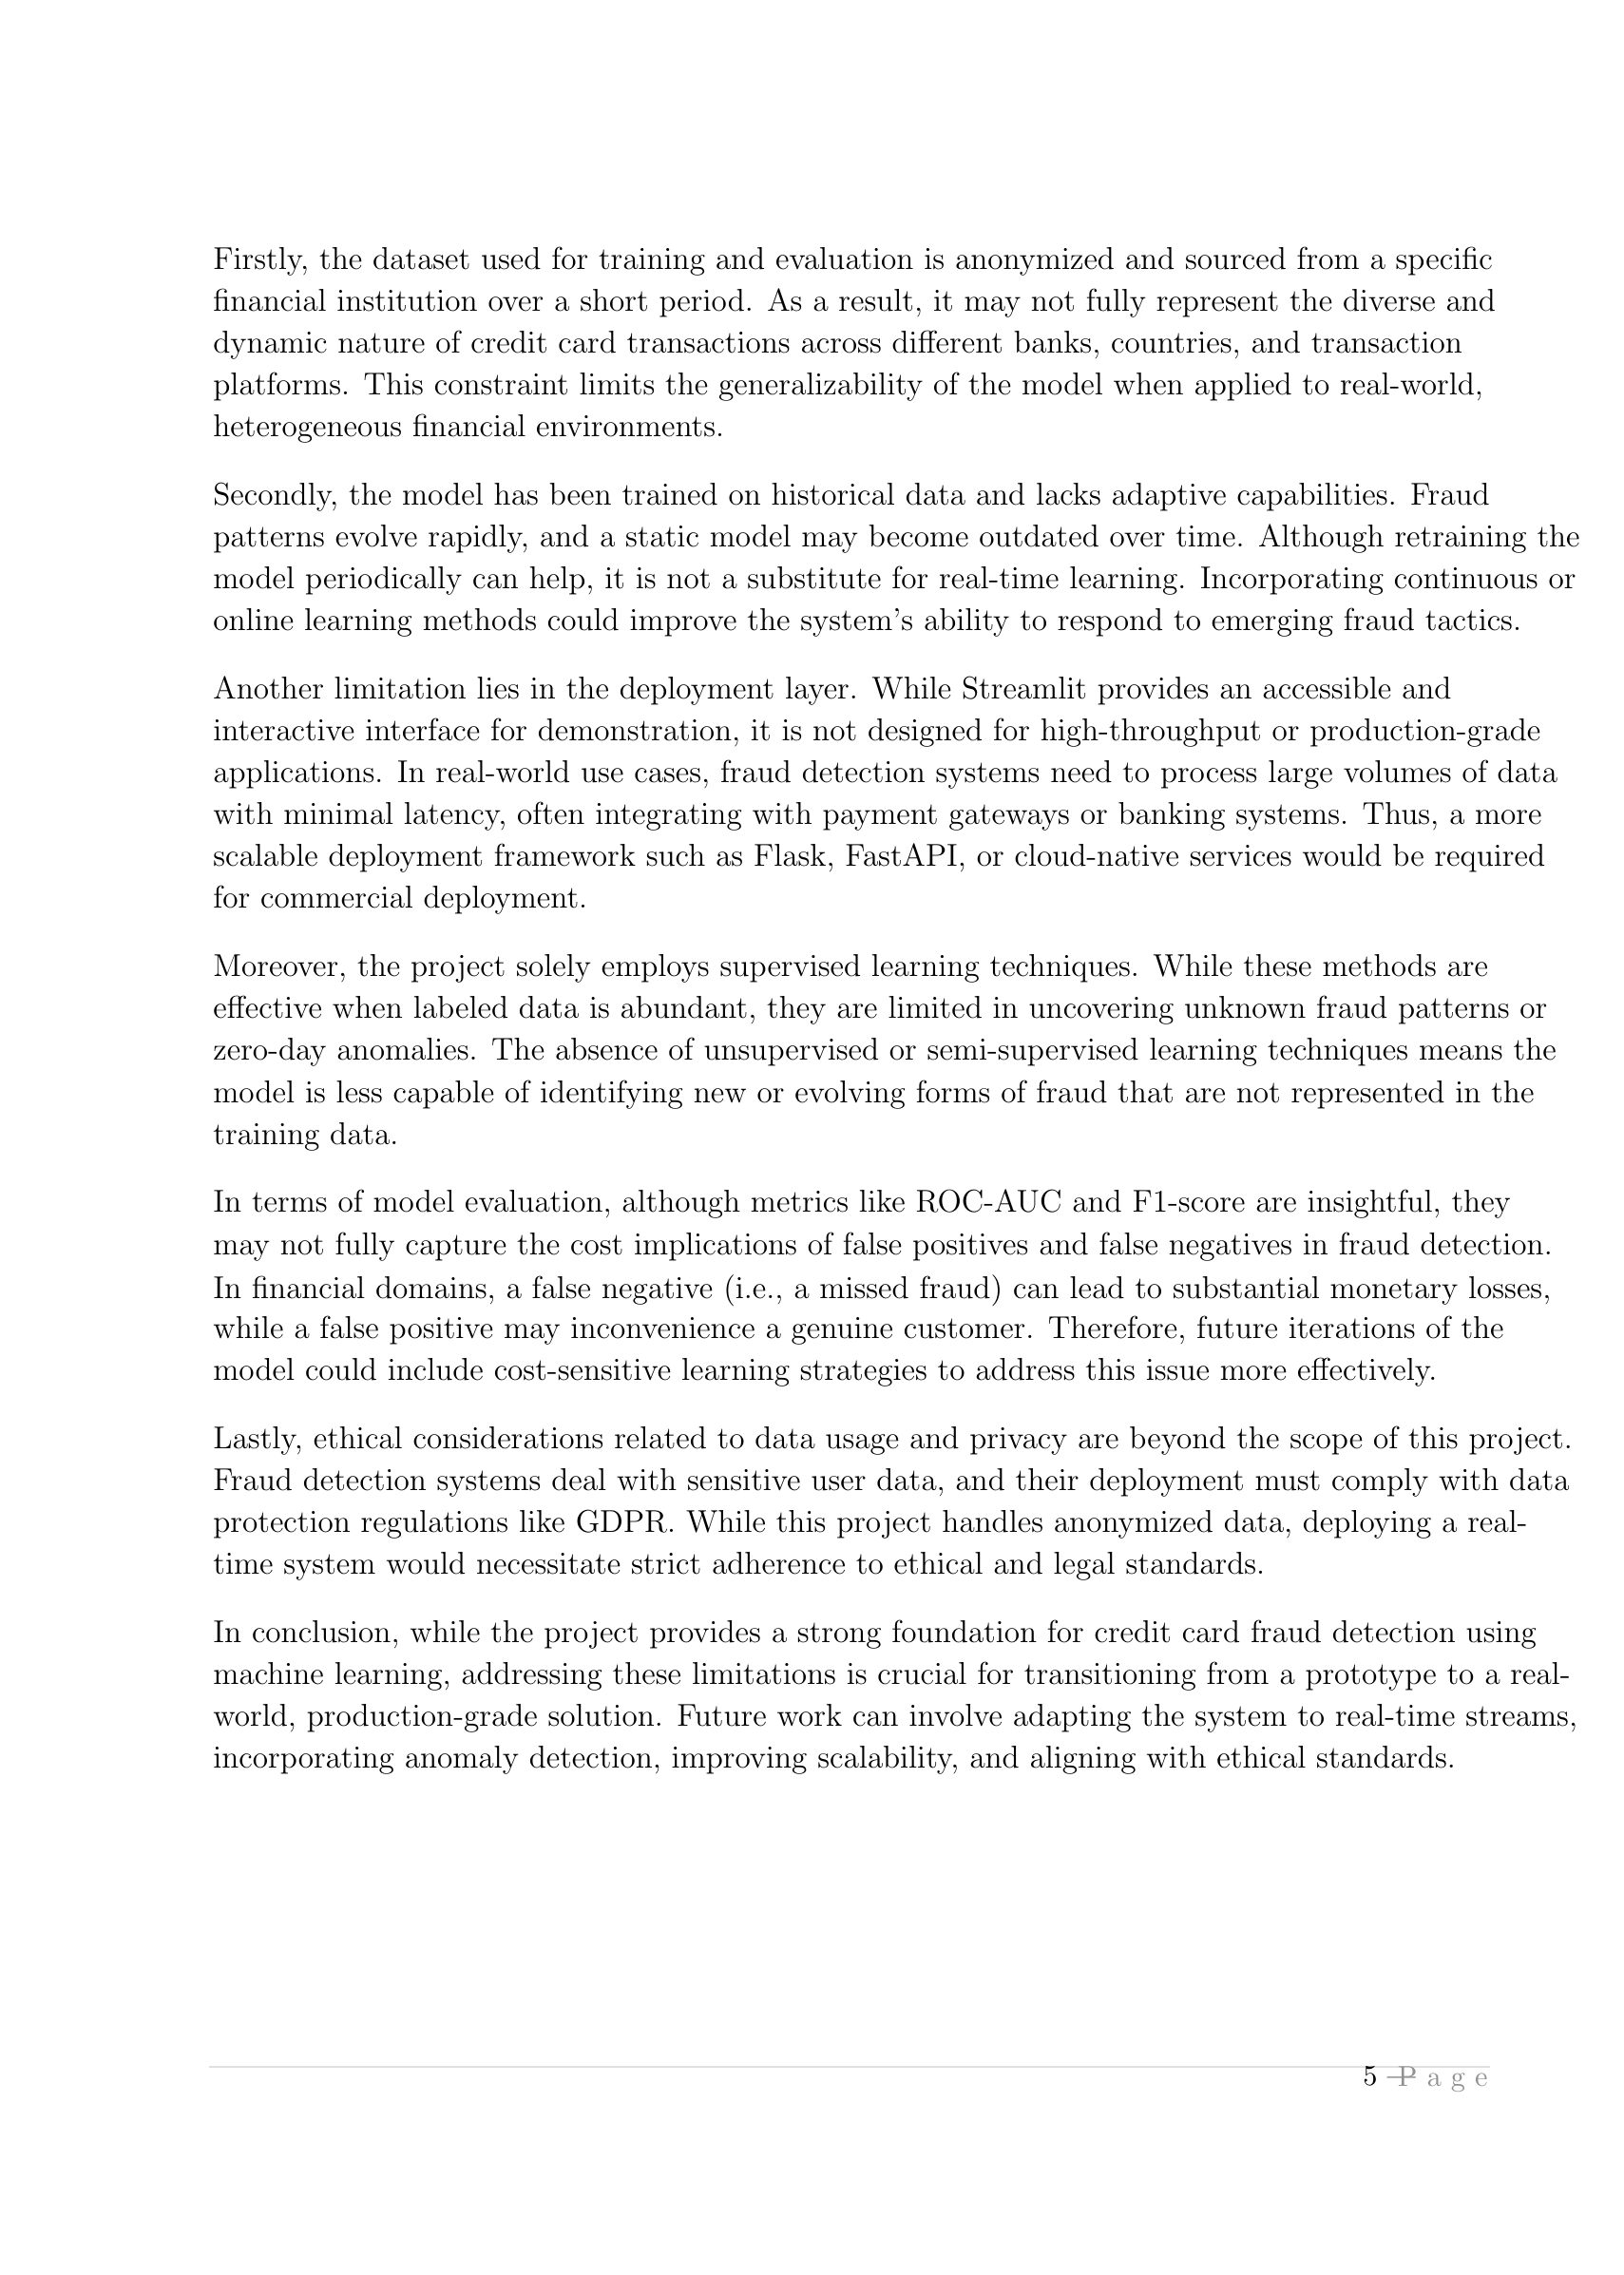
\begin{tikzpicture}[x=1bp,y=-1bp,inner sep=0pt,outer sep=0pt]
  \useasboundingbox (0,0) rectangle (595.20,841.92);
  \fill[fill=pdfcolor9] (69.38,772.78) rectangle (554.40,773.26);
  \node[anchor=north west,inner sep=0pt,outer sep=0pt] at (506.38,772.91) {{\fontsize{11.0bp}{13.2bp}\selectfont 5 | }};
  \node[anchor=north west,inner sep=0pt,outer sep=0pt] at (519.58,772.91) {{\fontsize{11.0bp}{13.2bp}\selectfont \textcolor{pdfcolor1}{P a g e}}};
  \node[anchor=north west,inner sep=0pt,outer sep=0pt] at (550.14,772.91) {{\fontsize{11.0bp}{13.2bp}\selectfont   }};
  \node[anchor=north west,inner sep=0pt,outer sep=0pt] at (70.82,83.62) {{\fontsize{12.0bp}{14.4bp}\selectfont Firstly, the dataset used for training and evaluation is anonymized and sourced from a specific }};
  \node[anchor=north west,inner sep=0pt,outer sep=0pt] at (70.82,99.46) {{\fontsize{12.0bp}{14.4bp}\selectfont financial institution over a short period. As a result, it may not fully represent the diverse and }};
  \node[anchor=north west,inner sep=0pt,outer sep=0pt] at (70.82,115.57) {{\fontsize{12.0bp}{14.4bp}\selectfont dynamic nature of credit card transactions across different banks, countries, and transaction }};
  \node[anchor=north west,inner sep=0pt,outer sep=0pt] at (70.82,131.41) {{\fontsize{12.0bp}{14.4bp}\selectfont platforms. This constraint limits the generalizability of the model when applied to real-world, }};
  \node[anchor=north west,inner sep=0pt,outer sep=0pt] at (70.82,147.25) {{\fontsize{12.0bp}{14.4bp}\selectfont heterogeneous financial environments. }};
  \node[anchor=north west,inner sep=0pt,outer sep=0pt] at (70.82,173.17) {{\fontsize{12.0bp}{14.4bp}\selectfont Secondly, the model has been trained on historical data and lacks adaptive capabilities. Fraud }};
  \node[anchor=north west,inner sep=0pt,outer sep=0pt] at (70.82,189.01) {{\fontsize{12.0bp}{14.4bp}\selectfont patterns evolve rapidly, and a static model may become outdated over time. Although retraining the }};
  \node[anchor=north west,inner sep=0pt,outer sep=0pt] at (70.82,204.87) {{\fontsize{12.0bp}{14.4bp}\selectfont model periodically can help, it is not a substitute for real-time learning. Incorporating continuous or }};
  \node[anchor=north west,inner sep=0pt,outer sep=0pt] at (70.82,220.71) {{\fontsize{12.0bp}{14.4bp}\selectfont online learning methods could improve the system's ability to respond to emerging fraud tactics. }};
  \node[anchor=north west,inner sep=0pt,outer sep=0pt] at (70.82,246.63) {{\fontsize{12.0bp}{14.4bp}\selectfont Another limitation lies in the deployment layer. While Streamlit provides an accessible and }};
  \node[anchor=north west,inner sep=0pt,outer sep=0pt] at (70.82,262.47) {{\fontsize{12.0bp}{14.4bp}\selectfont interactive interface for demonstration, it is not designed for high-throughput or production-grade }};
  \node[anchor=north west,inner sep=0pt,outer sep=0pt] at (70.82,278.31) {{\fontsize{12.0bp}{14.4bp}\selectfont applications. In real-world use cases, fraud detection systems need to process large volumes of data }};
  \node[anchor=north west,inner sep=0pt,outer sep=0pt] at (70.82,294.18) {{\fontsize{12.0bp}{14.4bp}\selectfont with minimal latency, often integrating with payment gateways or banking systems. Thus, a more }};
  \node[anchor=north west,inner sep=0pt,outer sep=0pt] at (70.82,310.02) {{\fontsize{12.0bp}{14.4bp}\selectfont scalable deployment framework such as Flask, FastAPI, or cloud-native services would be required }};
  \node[anchor=north west,inner sep=0pt,outer sep=0pt] at (70.82,325.86) {{\fontsize{12.0bp}{14.4bp}\selectfont for commercial deployment. }};
  \node[anchor=north west,inner sep=0pt,outer sep=0pt] at (70.82,351.78) {{\fontsize{12.0bp}{14.4bp}\selectfont Moreover, the project solely employs supervised learning techniques. While these methods are }};
  \node[anchor=north west,inner sep=0pt,outer sep=0pt] at (70.82,367.62) {{\fontsize{12.0bp}{14.4bp}\selectfont effective when labeled data is abundant, they are limited in uncovering unknown fraud patterns or }};
  \node[anchor=north west,inner sep=0pt,outer sep=0pt] at (70.82,383.48) {{\fontsize{12.0bp}{14.4bp}\selectfont zero-day anomalies. The absence of unsupervised or semi-supervised learning techniques means the }};
  \node[anchor=north west,inner sep=0pt,outer sep=0pt] at (70.82,399.56) {{\fontsize{12.0bp}{14.4bp}\selectfont model is less capable of identifying new or evolving forms of fraud that are not represented in the }};
  \node[anchor=north west,inner sep=0pt,outer sep=0pt] at (70.82,415.40) {{\fontsize{12.0bp}{14.4bp}\selectfont training data. }};
  \node[anchor=north west,inner sep=0pt,outer sep=0pt] at (70.82,441.08) {{\fontsize{12.0bp}{14.4bp}\selectfont In terms of model evaluation, although metrics like ROC-AUC and F1-score are insightful, they }};
  \node[anchor=north west,inner sep=0pt,outer sep=0pt] at (70.82,457.16) {{\fontsize{12.0bp}{14.4bp}\selectfont may not fully capture the cost implications of false positives and false negatives in fraud detection. }};
  \node[anchor=north west,inner sep=0pt,outer sep=0pt] at (70.82,473.02) {{\fontsize{12.0bp}{14.4bp}\selectfont In financial domains, a false negative (i.e., a missed fraud) can lead to substantial monetary losses, }};
  \node[anchor=north west,inner sep=0pt,outer sep=0pt] at (70.82,488.86) {{\fontsize{12.0bp}{14.4bp}\selectfont while a false positive may inconvenience a genuine customer. Therefore, future iterations of the }};
  \node[anchor=north west,inner sep=0pt,outer sep=0pt] at (70.82,504.70) {{\fontsize{12.0bp}{14.4bp}\selectfont model could include cost-sensitive learning strategies to address this issue more effectively. }};
  \node[anchor=north west,inner sep=0pt,outer sep=0pt] at (70.82,530.62) {{\fontsize{12.0bp}{14.4bp}\selectfont Lastly, ethical considerations related to data usage and privacy are beyond the scope of this project. }};
  \node[anchor=north west,inner sep=0pt,outer sep=0pt] at (70.82,546.49) {{\fontsize{12.0bp}{14.4bp}\selectfont Fraud detection systems deal with sensitive user data, and their deployment must comply with data }};
  \node[anchor=north west,inner sep=0pt,outer sep=0pt] at (70.82,562.33) {{\fontsize{12.0bp}{14.4bp}\selectfont protection regulations like GDPR. While this project handles anonymized data, deploying a real-}};
  \node[anchor=north west,inner sep=0pt,outer sep=0pt] at (70.82,578.17) {{\fontsize{12.0bp}{14.4bp}\selectfont time system would necessitate strict adherence to ethical and legal standards. }};
  \node[anchor=north west,inner sep=0pt,outer sep=0pt] at (70.82,604.09) {{\fontsize{12.0bp}{14.4bp}\selectfont In conclusion, while the project provides a strong foundation for credit card fraud detection using }};
  \node[anchor=north west,inner sep=0pt,outer sep=0pt] at (70.82,619.93) {{\fontsize{12.0bp}{14.4bp}\selectfont machine learning, addressing these limitations is crucial for transitioning from a prototype to a real-}};
  \node[anchor=north west,inner sep=0pt,outer sep=0pt] at (70.82,635.79) {{\fontsize{12.0bp}{14.4bp}\selectfont world, production-grade solution. Future work can involve adapting the system to real-time streams, }};
  \node[anchor=north west,inner sep=0pt,outer sep=0pt] at (70.82,651.63) {{\fontsize{12.0bp}{14.4bp}\selectfont incorporating anomaly detection, improving scalability, and aligning with ethical standards. }};
\end{tikzpicture}
\newpage
\noindent
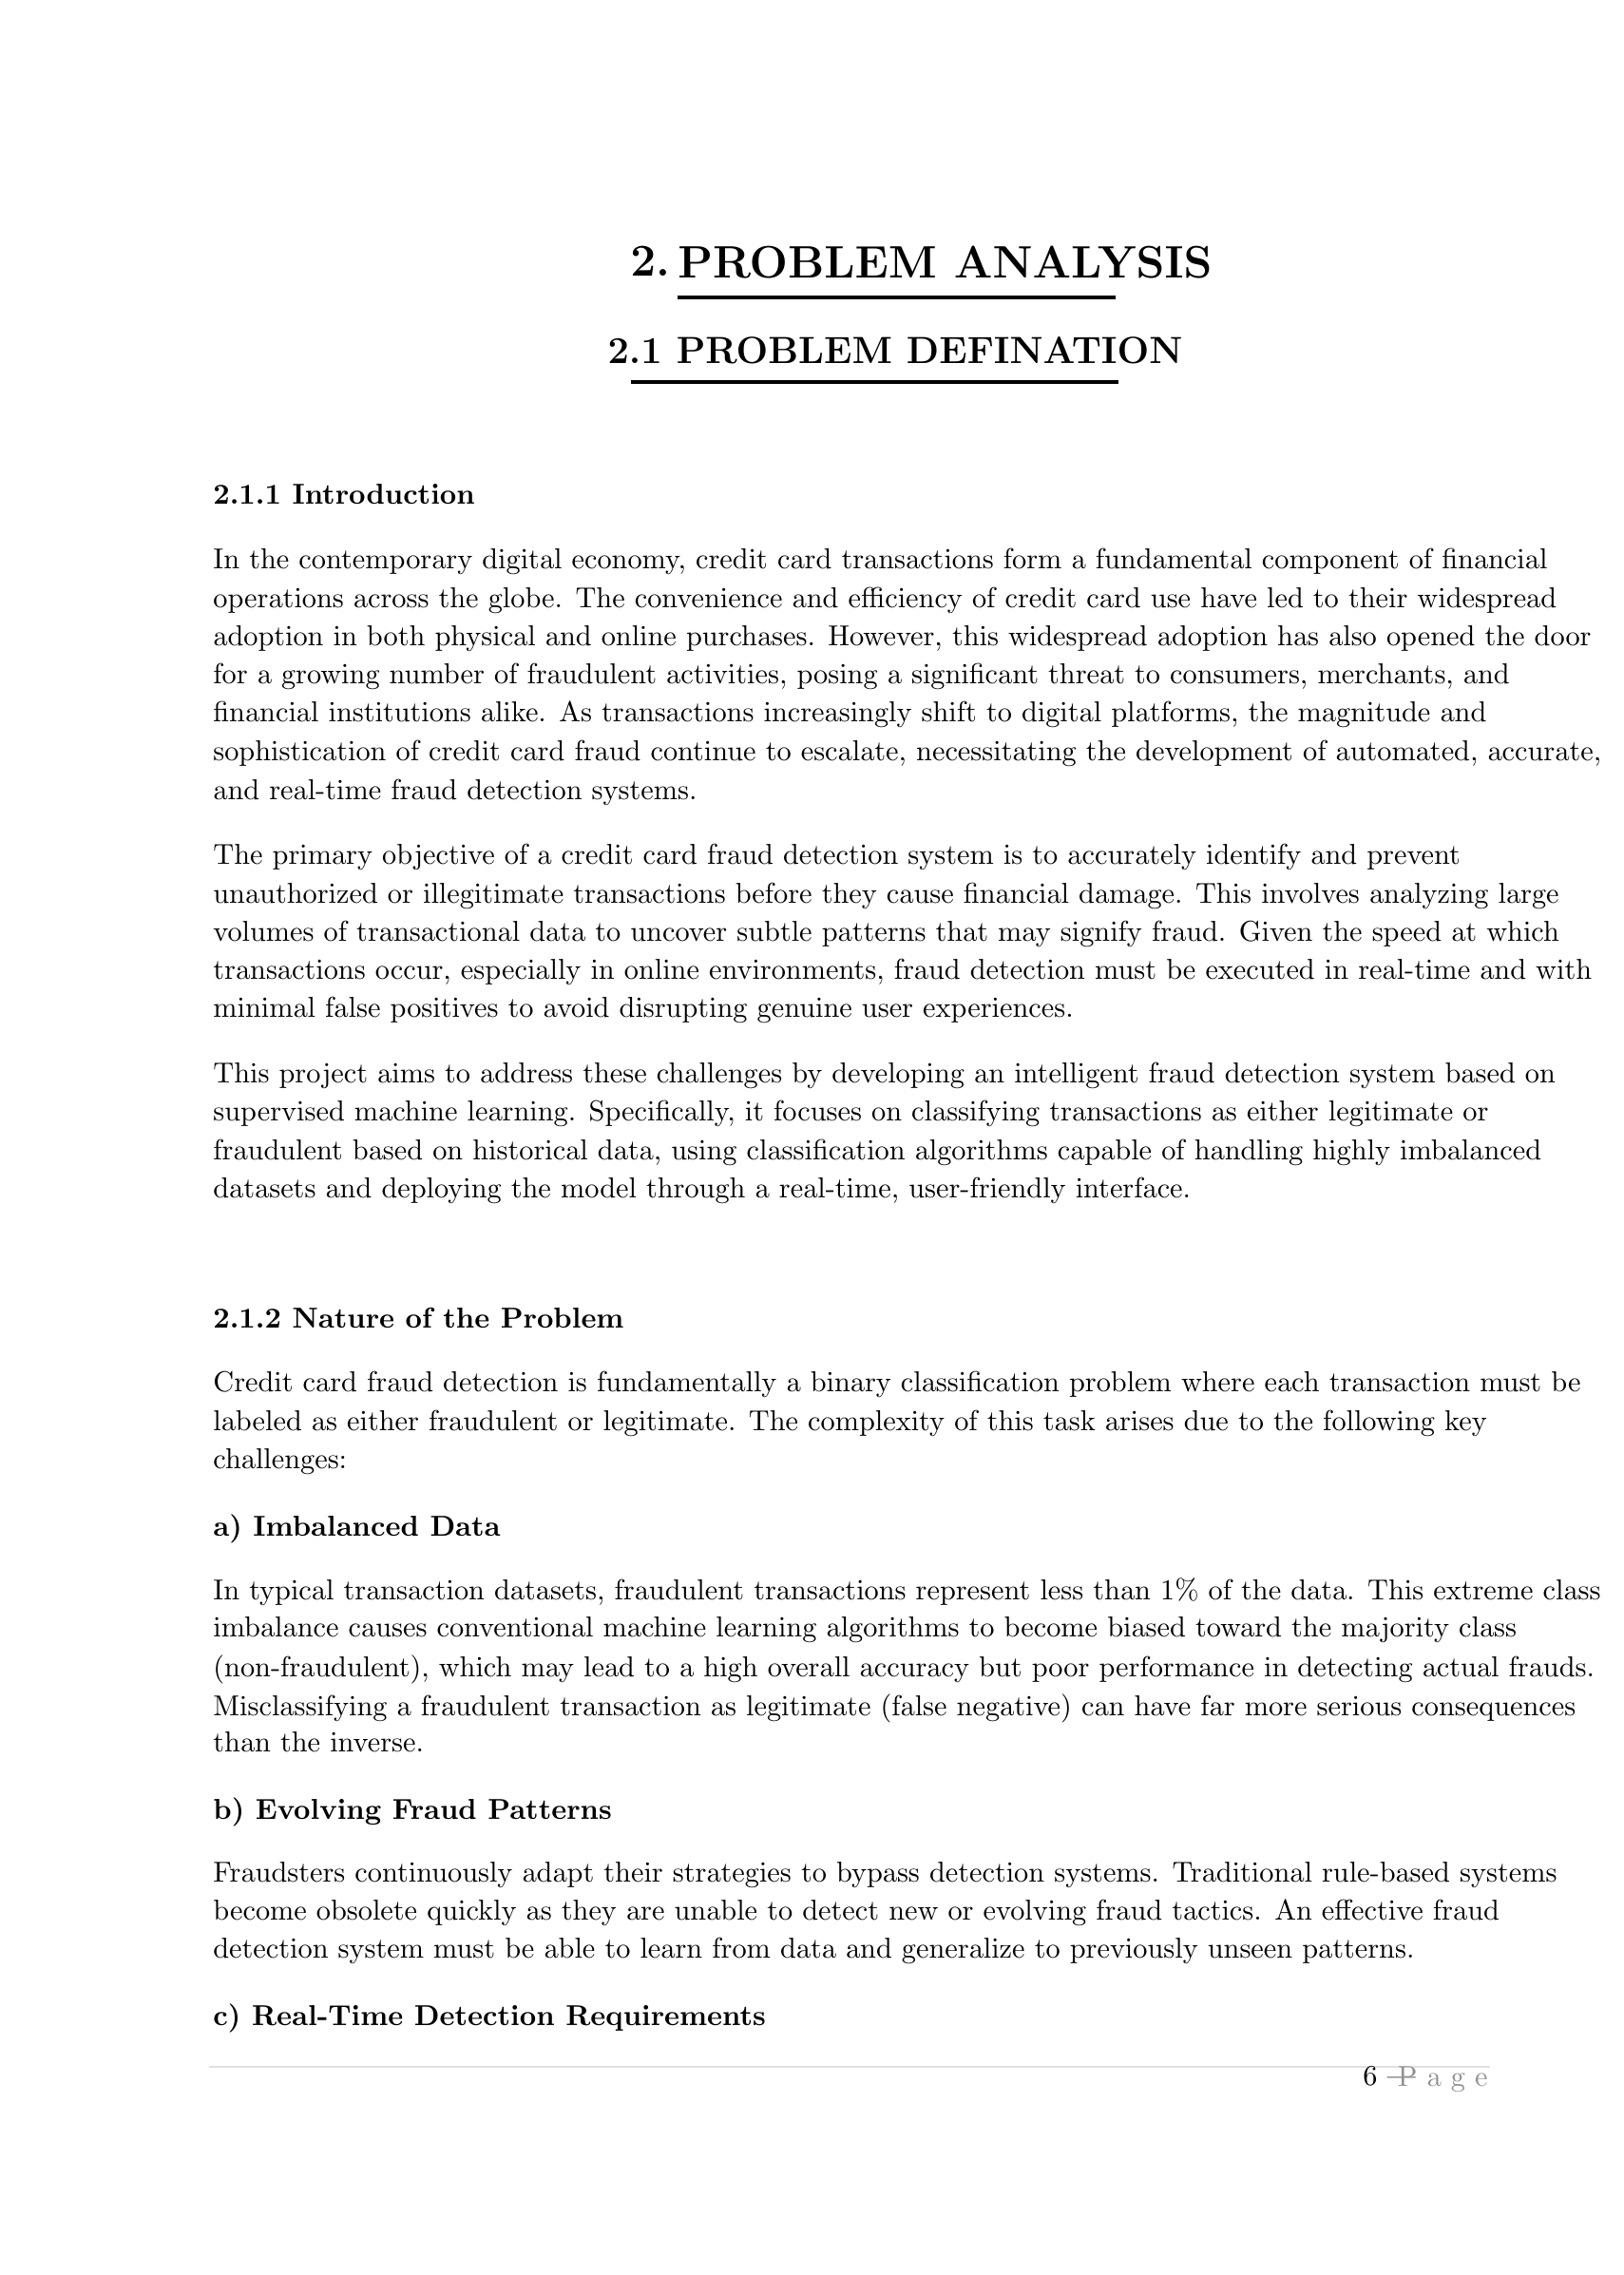
\begin{tikzpicture}[x=1bp,y=-1bp,inner sep=0pt,outer sep=0pt]
  \useasboundingbox (0,0) rectangle (595.20,841.92);
  \fill[fill=pdfcolor9] (69.38,772.78) rectangle (554.40,773.26);
  \fill[fill=black] (246.82,102.02) rectangle (412.73,103.46);
  \fill[fill=black] (229.06,133.97) rectangle (413.69,135.41);
  \node[anchor=north west,inner sep=0pt,outer sep=0pt] at (506.38,772.91) {{\fontsize{11.0bp}{13.2bp}\selectfont 6 | }};
  \node[anchor=north west,inner sep=0pt,outer sep=0pt] at (519.58,772.91) {{\fontsize{11.0bp}{13.2bp}\selectfont \textcolor{pdfcolor1}{P a g e}}};
  \node[anchor=north west,inner sep=0pt,outer sep=0pt] at (550.14,772.91) {{\fontsize{11.0bp}{13.2bp}\selectfont   }};
  \node[anchor=north west,inner sep=0pt,outer sep=0pt] at (228.82,83.55) {{\fontsize{16.1bp}{19.3bp}\selectfont \textbf{2.}}};
  \node[anchor=north west,inner sep=0pt,outer sep=0pt] at (240.82,83.13) {\textsf{{\fontsize{16.1bp}{19.3bp}\selectfont \textbf{ }}}};
  \node[anchor=north west,inner sep=0pt,outer sep=0pt] at (246.82,83.55) {{\fontsize{16.1bp}{19.3bp}\selectfont \textbf{PROBLEM ANALYSIS }}};
  \node[anchor=north west,inner sep=0pt,outer sep=0pt] at (214.90,118.00) {{\fontsize{13.9bp}{16.7bp}\selectfont \textbf{    2.1 PROBLEM DEFINATION  }}};
  \node[anchor=north west,inner sep=0pt,outer sep=0pt] at (70.82,159.25) {{\fontsize{12.0bp}{14.4bp}\selectfont  }};
  \node[anchor=north west,inner sep=0pt,outer sep=0pt] at (70.82,173.56) {{\fontsize{11.0bp}{13.2bp}\selectfont \textbf{2.1.1 Introduction }}};
  \node[anchor=north west,inner sep=0pt,outer sep=0pt] at (70.82,197.94) {{\fontsize{11.0bp}{13.2bp}\selectfont In the contemporary digital economy, credit card transactions form a fundamental component of financial }};
  \node[anchor=north west,inner sep=0pt,outer sep=0pt] at (70.82,212.60) {{\fontsize{11.0bp}{13.2bp}\selectfont operations across the globe. The convenience and efficiency of credit card use have led to their widespread }};
  \node[anchor=north west,inner sep=0pt,outer sep=0pt] at (70.82,227.00) {{\fontsize{11.0bp}{13.2bp}\selectfont adoption in both physical and online purchases. However, this widespread adoption has also opened the door }};
  \node[anchor=north west,inner sep=0pt,outer sep=0pt] at (70.82,241.64) {{\fontsize{11.0bp}{13.2bp}\selectfont for a growing number of fraudulent activities, posing a significant threat to consumers, merchants, and }};
  \node[anchor=north west,inner sep=0pt,outer sep=0pt] at (70.82,256.04) {{\fontsize{11.0bp}{13.2bp}\selectfont financial institutions alike. As transactions increasingly shift to digital platforms, the magnitude and }};
  \node[anchor=north west,inner sep=0pt,outer sep=0pt] at (70.82,270.68) {{\fontsize{11.0bp}{13.2bp}\selectfont sophistication of credit card fraud continue to escalate, necessitating the development of automated, accurate, }};
  \node[anchor=north west,inner sep=0pt,outer sep=0pt] at (70.82,285.32) {{\fontsize{11.0bp}{13.2bp}\selectfont and real-time fraud detection systems. }};
  \node[anchor=north west,inner sep=0pt,outer sep=0pt] at (70.82,309.83) {{\fontsize{11.0bp}{13.2bp}\selectfont The primary objective of a credit card fraud detection system is to accurately identify and prevent }};
  \node[anchor=north west,inner sep=0pt,outer sep=0pt] at (70.82,324.47) {{\fontsize{11.0bp}{13.2bp}\selectfont unauthorized or illegitimate transactions before they cause financial damage. This involves analyzing large }};
  \node[anchor=north west,inner sep=0pt,outer sep=0pt] at (70.82,338.87) {{\fontsize{11.0bp}{13.2bp}\selectfont volumes of transactional data to uncover subtle patterns that may signify fraud. Given the speed at which }};
  \node[anchor=north west,inner sep=0pt,outer sep=0pt] at (70.82,353.51) {{\fontsize{11.0bp}{13.2bp}\selectfont transactions occur, especially in online environments, fraud detection must be executed in real-time and with }};
  \node[anchor=north west,inner sep=0pt,outer sep=0pt] at (70.82,367.91) {{\fontsize{11.0bp}{13.2bp}\selectfont minimal false positives to avoid disrupting genuine user experiences. }};
  \node[anchor=north west,inner sep=0pt,outer sep=0pt] at (70.82,392.65) {{\fontsize{11.0bp}{13.2bp}\selectfont This project aims to address these challenges by developing an intelligent fraud detection system based on }};
  \node[anchor=north west,inner sep=0pt,outer sep=0pt] at (70.82,407.05) {{\fontsize{11.0bp}{13.2bp}\selectfont supervised machine learning. Specifically, it focuses on classifying transactions as either legitimate or }};
  \node[anchor=north west,inner sep=0pt,outer sep=0pt] at (70.82,421.69) {{\fontsize{11.0bp}{13.2bp}\selectfont fraudulent based on historical data, using classification algorithms capable of handling highly imbalanced }};
  \node[anchor=north west,inner sep=0pt,outer sep=0pt] at (70.82,436.09) {{\fontsize{11.0bp}{13.2bp}\selectfont datasets and deploying the model through a real-time, user-friendly interface. }};
  \node[anchor=north west,inner sep=0pt,outer sep=0pt] at (70.82,485.41) {{\fontsize{11.0bp}{13.2bp}\selectfont \textbf{2.1.2 Nature of the Problem }}};
  \node[anchor=north west,inner sep=0pt,outer sep=0pt] at (70.82,509.79) {{\fontsize{11.0bp}{13.2bp}\selectfont Credit card fraud detection is fundamentally a binary classification problem where each transaction must be }};
  \node[anchor=north west,inner sep=0pt,outer sep=0pt] at (70.82,524.43) {{\fontsize{11.0bp}{13.2bp}\selectfont labeled as either fraudulent or legitimate. The complexity of this task arises due to the following key }};
  \node[anchor=north west,inner sep=0pt,outer sep=0pt] at (70.82,538.83) {{\fontsize{11.0bp}{13.2bp}\selectfont challenges: }};
  \node[anchor=north west,inner sep=0pt,outer sep=0pt] at (70.82,563.68) {{\fontsize{11.0bp}{13.2bp}\selectfont \textbf{a) Imbalanced Data }}};
  \node[anchor=north west,inner sep=0pt,outer sep=0pt] at (70.82,588.06) {{\fontsize{11.0bp}{13.2bp}\selectfont In typical transaction datasets, fraudulent transactions represent less than 1\% of the data. This extreme class }};
  \node[anchor=north west,inner sep=0pt,outer sep=0pt] at (70.82,602.70) {{\fontsize{11.0bp}{13.2bp}\selectfont imbalance causes conventional machine learning algorithms to become biased toward the majority class }};
  \node[anchor=north west,inner sep=0pt,outer sep=0pt] at (70.82,617.10) {{\fontsize{11.0bp}{13.2bp}\selectfont (non-fraudulent), which may lead to a high overall accuracy but poor performance in detecting actual frauds. }};
  \node[anchor=north west,inner sep=0pt,outer sep=0pt] at (70.82,631.76) {{\fontsize{11.0bp}{13.2bp}\selectfont Misclassifying a fraudulent transaction as legitimate (false negative) can have far more serious consequences }};
  \node[anchor=north west,inner sep=0pt,outer sep=0pt] at (70.82,646.16) {{\fontsize{11.0bp}{13.2bp}\selectfont than the inverse. }};
  \node[anchor=north west,inner sep=0pt,outer sep=0pt] at (70.82,670.98) {{\fontsize{11.0bp}{13.2bp}\selectfont \textbf{b) Evolving Fraud Patterns }}};
  \node[anchor=north west,inner sep=0pt,outer sep=0pt] at (70.82,695.36) {{\fontsize{11.0bp}{13.2bp}\selectfont Fraudsters continuously adapt their strategies to bypass detection systems. Traditional rule-based systems }};
  \node[anchor=north west,inner sep=0pt,outer sep=0pt] at (70.82,710.00) {{\fontsize{11.0bp}{13.2bp}\selectfont become obsolete quickly as they are unable to detect new or evolving fraud tactics. An effective fraud }};
  \node[anchor=north west,inner sep=0pt,outer sep=0pt] at (70.82,724.43) {{\fontsize{11.0bp}{13.2bp}\selectfont detection system must be able to learn from data and generalize to previously unseen patterns. }};
  \node[anchor=north west,inner sep=0pt,outer sep=0pt] at (70.82,749.25) {{\fontsize{11.0bp}{13.2bp}\selectfont \textbf{c) Real-Time Detection Requirements }}};
\end{tikzpicture}
\newpage
\noindent
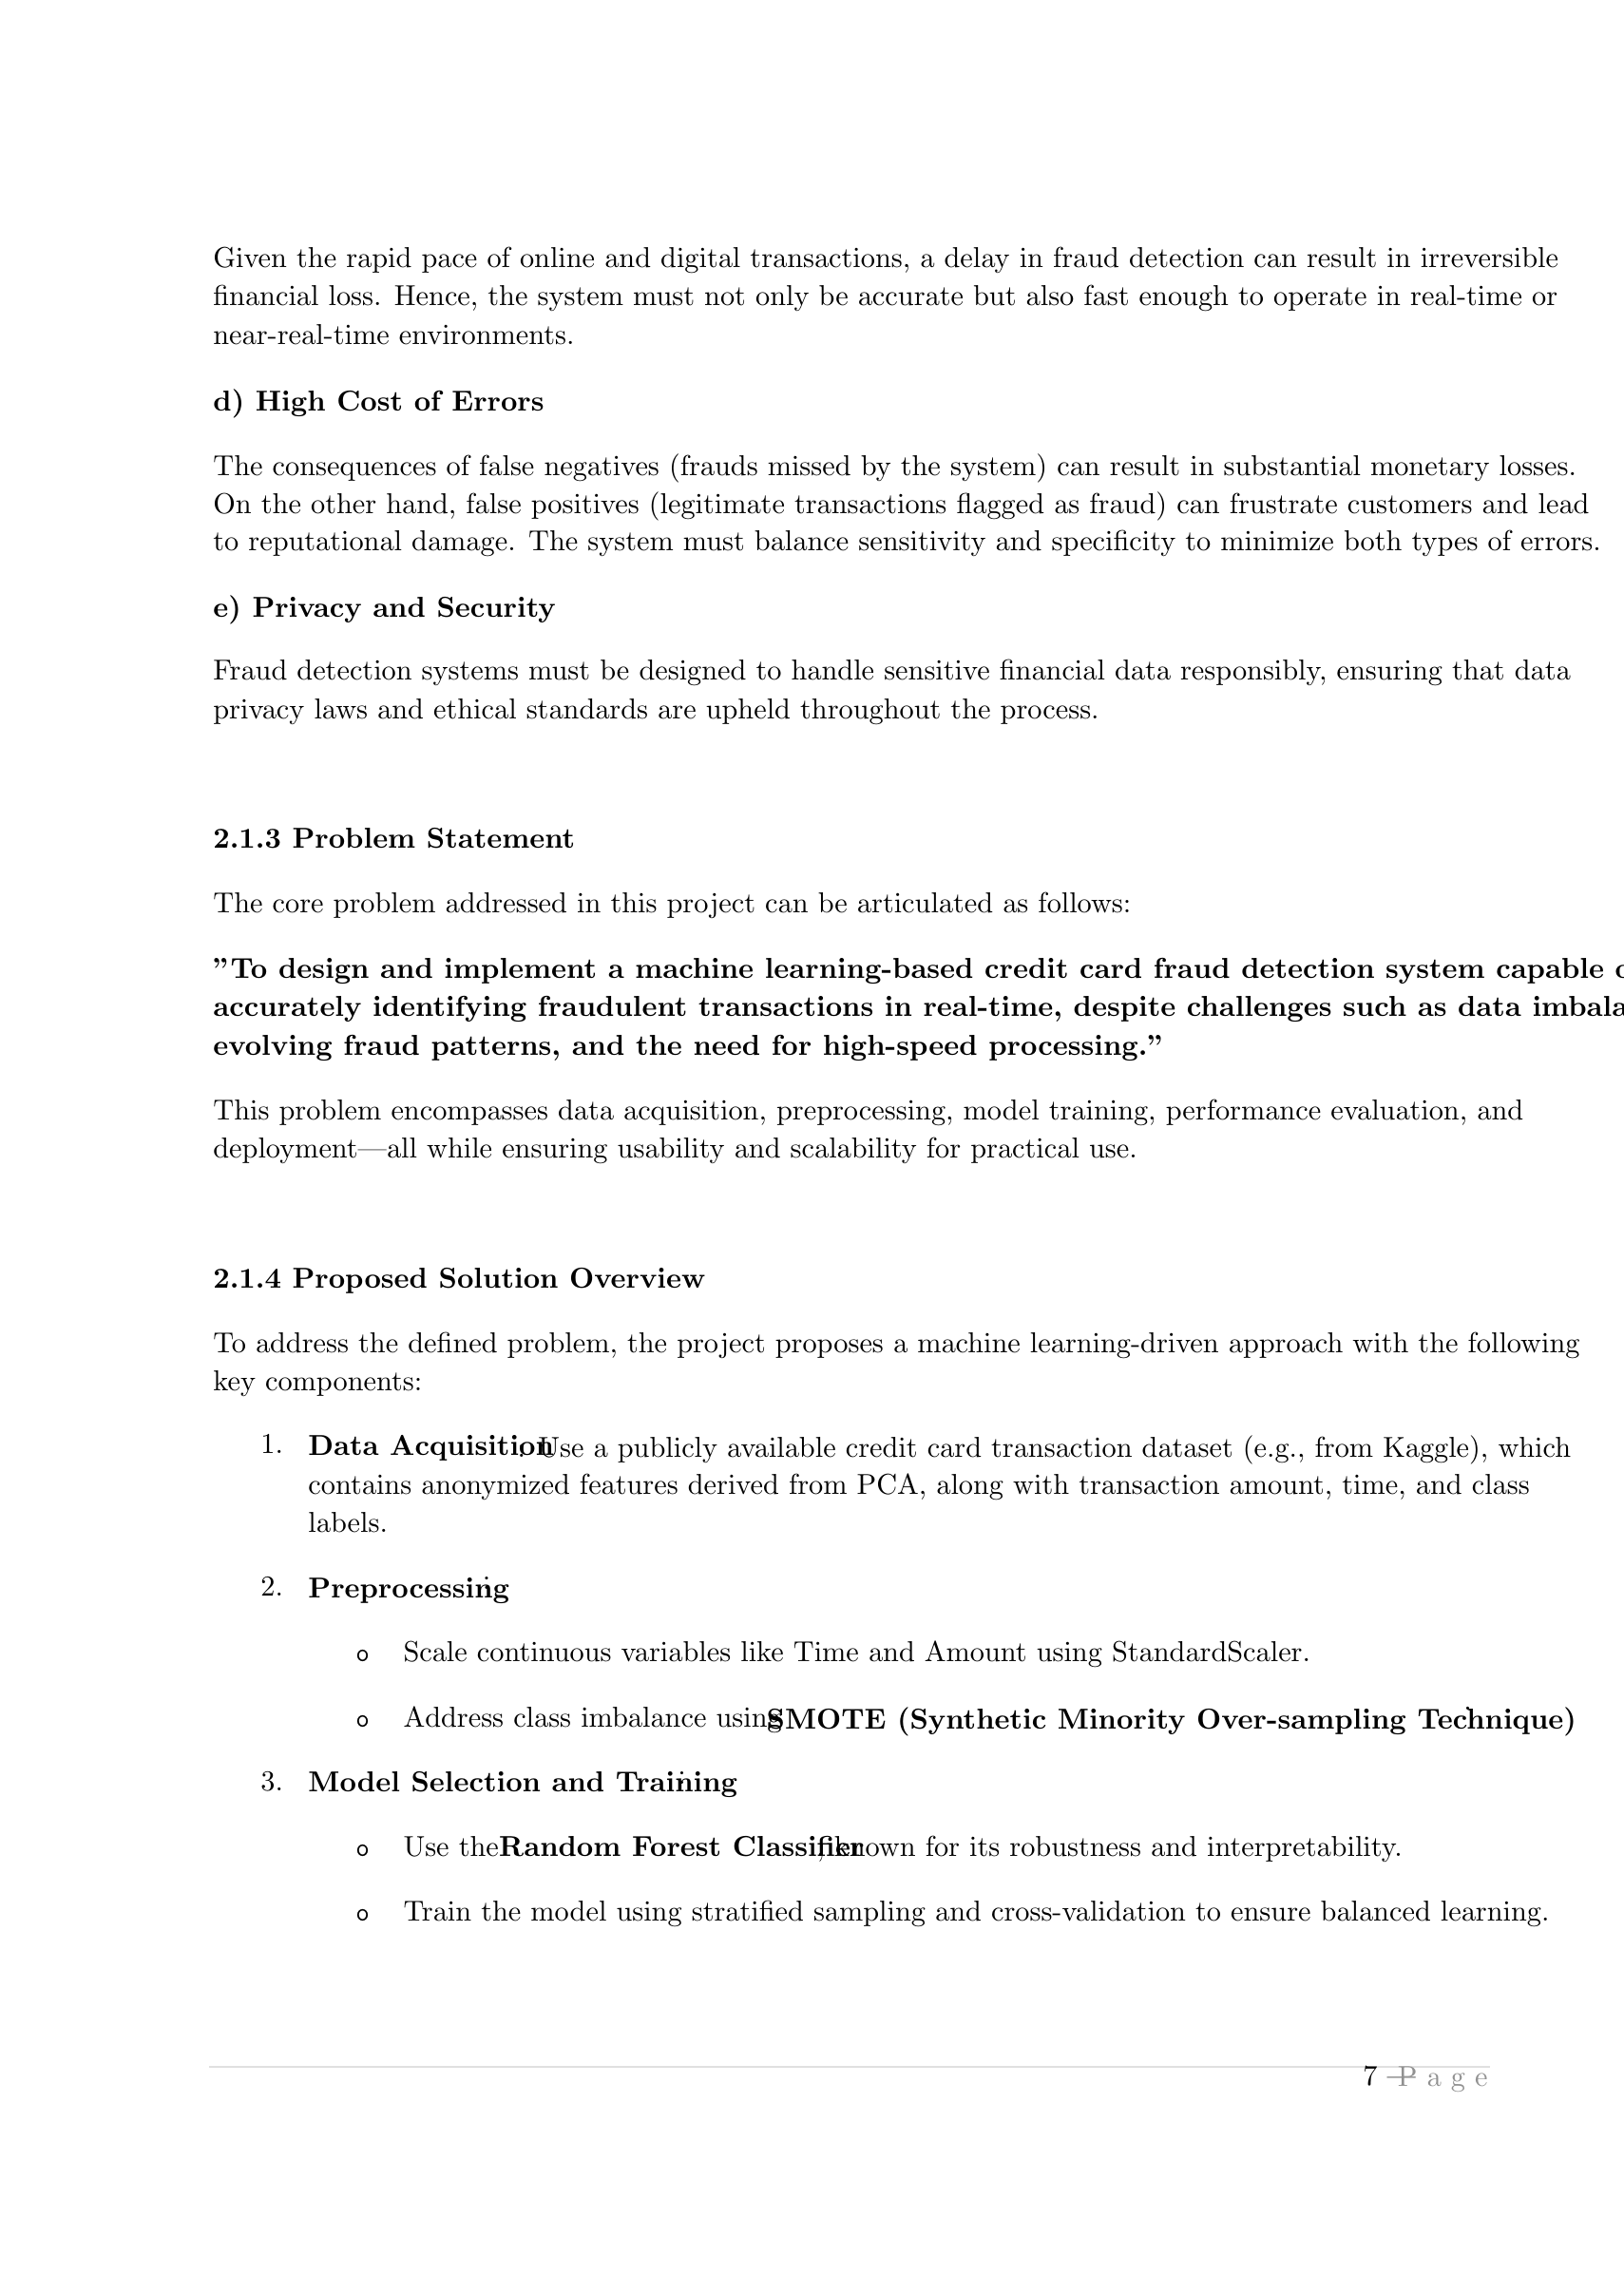
\begin{tikzpicture}[x=1bp,y=-1bp,inner sep=0pt,outer sep=0pt]
  \useasboundingbox (0,0) rectangle (595.20,841.92);
  \fill[fill=pdfcolor9] (69.38,772.78) rectangle (554.40,773.26);
  \node[anchor=north west,inner sep=0pt,outer sep=0pt] at (506.38,772.91) {{\fontsize{11.0bp}{13.2bp}\selectfont 7 | }};
  \node[anchor=north west,inner sep=0pt,outer sep=0pt] at (519.58,772.91) {{\fontsize{11.0bp}{13.2bp}\selectfont \textcolor{pdfcolor1}{P a g e}}};
  \node[anchor=north west,inner sep=0pt,outer sep=0pt] at (550.14,772.91) {{\fontsize{11.0bp}{13.2bp}\selectfont   }};
  \node[anchor=north west,inner sep=0pt,outer sep=0pt] at (70.82,83.67) {{\fontsize{11.0bp}{13.2bp}\selectfont Given the rapid pace of online and digital transactions, a delay in fraud detection can result in irreversible }};
  \node[anchor=north west,inner sep=0pt,outer sep=0pt] at (70.82,98.31) {{\fontsize{11.0bp}{13.2bp}\selectfont financial loss. Hence, the system must not only be accurate but also fast enough to operate in real-time or }};
  \node[anchor=north west,inner sep=0pt,outer sep=0pt] at (70.82,112.95) {{\fontsize{11.0bp}{13.2bp}\selectfont near-real-time environments. }};
  \node[anchor=north west,inner sep=0pt,outer sep=0pt] at (70.82,137.56) {{\fontsize{11.0bp}{13.2bp}\selectfont \textbf{d) High Cost of Errors }}};
  \node[anchor=north west,inner sep=0pt,outer sep=0pt] at (70.82,161.94) {{\fontsize{11.0bp}{13.2bp}\selectfont The consequences of false negatives (frauds missed by the system) can result in substantial monetary losses. }};
  \node[anchor=north west,inner sep=0pt,outer sep=0pt] at (70.82,176.58) {{\fontsize{11.0bp}{13.2bp}\selectfont On the other hand, false positives (legitimate transactions flagged as fraud) can frustrate customers and lead }};
  \node[anchor=north west,inner sep=0pt,outer sep=0pt] at (70.82,190.98) {{\fontsize{11.0bp}{13.2bp}\selectfont to reputational damage. The system must balance sensitivity and specificity to minimize both types of errors. }};
  \node[anchor=north west,inner sep=0pt,outer sep=0pt] at (70.82,215.82) {{\fontsize{11.0bp}{13.2bp}\selectfont \textbf{e) Privacy and Security }}};
  \node[anchor=north west,inner sep=0pt,outer sep=0pt] at (70.82,240.20) {{\fontsize{11.0bp}{13.2bp}\selectfont Fraud detection systems must be designed to handle sensitive financial data responsibly, ensuring that data }};
  \node[anchor=north west,inner sep=0pt,outer sep=0pt] at (70.82,254.84) {{\fontsize{11.0bp}{13.2bp}\selectfont privacy laws and ethical standards are upheld throughout the process. }};
  \node[anchor=north west,inner sep=0pt,outer sep=0pt] at (70.82,303.93) {{\fontsize{11.0bp}{13.2bp}\selectfont \textbf{2.1.3 Problem Statement }}};
  \node[anchor=north west,inner sep=0pt,outer sep=0pt] at (70.82,328.31) {{\fontsize{11.0bp}{13.2bp}\selectfont The core problem addressed in this project can be articulated as follows: }};
  \node[anchor=north west,inner sep=0pt,outer sep=0pt] at (70.82,353.13) {{\fontsize{11.0bp}{13.2bp}\selectfont \textbf{''To design and implement a machine learning-based credit card fraud detection system capable of }}};
  \node[anchor=north west,inner sep=0pt,outer sep=0pt] at (70.82,367.53) {{\fontsize{11.0bp}{13.2bp}\selectfont \textbf{accurately identifying fraudulent transactions in real-time, despite challenges such as data imbalance, }}};
  \node[anchor=north west,inner sep=0pt,outer sep=0pt] at (70.82,382.19) {{\fontsize{11.0bp}{13.2bp}\selectfont \textbf{evolving fraud patterns, and the need for high-speed processing.''}}};
  \node[anchor=north west,inner sep=0pt,outer sep=0pt] at (377.69,382.09) {{\fontsize{11.0bp}{13.2bp}\selectfont  }};
  \node[anchor=north west,inner sep=0pt,outer sep=0pt] at (70.82,406.57) {{\fontsize{11.0bp}{13.2bp}\selectfont This problem encompasses data acquisition, preprocessing, model training, performance evaluation, and }};
  \node[anchor=north west,inner sep=0pt,outer sep=0pt] at (70.82,421.21) {{\fontsize{11.0bp}{13.2bp}\selectfont deployment---all while ensuring usability and scalability for practical use. }};
  \node[anchor=north west,inner sep=0pt,outer sep=0pt] at (70.82,470.29) {{\fontsize{11.0bp}{13.2bp}\selectfont \textbf{2.1.4 Proposed Solution Overview }}};
  \node[anchor=north west,inner sep=0pt,outer sep=0pt] at (70.82,494.91) {{\fontsize{11.0bp}{13.2bp}\selectfont To address the defined problem, the project proposes a machine learning-driven approach with the following }};
  \node[anchor=north west,inner sep=0pt,outer sep=0pt] at (70.82,509.31) {{\fontsize{11.0bp}{13.2bp}\selectfont key components: }};
  \node[anchor=north west,inner sep=0pt,outer sep=0pt] at (88.85,533.79) {{\fontsize{11.0bp}{13.2bp}\selectfont 1.}};
  \node[anchor=north west,inner sep=0pt,outer sep=0pt] at (97.01,533.55) {\textsf{{\fontsize{11.0bp}{13.2bp}\selectfont  }}};
  \node[anchor=north west,inner sep=0pt,outer sep=0pt] at (106.85,533.89) {{\fontsize{11.0bp}{13.2bp}\selectfont \textbf{Data Acquisition}}};
  \node[anchor=north west,inner sep=0pt,outer sep=0pt] at (186.07,533.79) {{\fontsize{11.0bp}{13.2bp}\selectfont : Use a publicly available credit card transaction dataset (e.g., from Kaggle), which }};
  \node[anchor=north west,inner sep=0pt,outer sep=0pt] at (106.85,548.46) {{\fontsize{11.0bp}{13.2bp}\selectfont contains anonymized features derived from PCA, along with transaction amount, time, and class }};
  \node[anchor=north west,inner sep=0pt,outer sep=0pt] at (106.85,563.10) {{\fontsize{11.0bp}{13.2bp}\selectfont labels. }};
  \node[anchor=north west,inner sep=0pt,outer sep=0pt] at (88.85,587.58) {{\fontsize{11.0bp}{13.2bp}\selectfont 2.}};
  \node[anchor=north west,inner sep=0pt,outer sep=0pt] at (97.01,587.34) {\textsf{{\fontsize{11.0bp}{13.2bp}\selectfont  }}};
  \node[anchor=north west,inner sep=0pt,outer sep=0pt] at (106.85,587.68) {{\fontsize{11.0bp}{13.2bp}\selectfont \textbf{Preprocessing}}};
  \node[anchor=north west,inner sep=0pt,outer sep=0pt] at (172.87,587.58) {{\fontsize{11.0bp}{13.2bp}\selectfont : }};
  \node[anchor=north west,inner sep=0pt,outer sep=0pt] at (124.85,615.30) {\texttt{{\fontsize{10.1bp}{12.1bp}\selectfont o}}};
  \node[anchor=north west,inner sep=0pt,outer sep=0pt] at (130.85,612.85) {\textsf{{\fontsize{10.1bp}{12.1bp}\selectfont  }}};
  \node[anchor=north west,inner sep=0pt,outer sep=0pt] at (142.87,612.06) {{\fontsize{11.0bp}{13.2bp}\selectfont Scale continuous variables like Time and Amount using StandardScaler. }};
  \node[anchor=north west,inner sep=0pt,outer sep=0pt] at (124.85,640.04) {\texttt{{\fontsize{10.1bp}{12.1bp}\selectfont o}}};
  \node[anchor=north west,inner sep=0pt,outer sep=0pt] at (130.85,637.59) {\textsf{{\fontsize{10.1bp}{12.1bp}\selectfont  }}};
  \node[anchor=north west,inner sep=0pt,outer sep=0pt] at (142.87,636.80) {{\fontsize{11.0bp}{13.2bp}\selectfont Address class imbalance using }};
  \node[anchor=north west,inner sep=0pt,outer sep=0pt] at (280.44,636.90) {{\fontsize{11.0bp}{13.2bp}\selectfont \textbf{SMOTE (Synthetic Minority Over-sampling Technique)}}};
  \node[anchor=north west,inner sep=0pt,outer sep=0pt] at (544.56,636.80) {{\fontsize{11.0bp}{13.2bp}\selectfont . }};
  \node[anchor=north west,inner sep=0pt,outer sep=0pt] at (88.85,661.28) {{\fontsize{11.0bp}{13.2bp}\selectfont 3.}};
  \node[anchor=north west,inner sep=0pt,outer sep=0pt] at (97.01,661.04) {\textsf{{\fontsize{11.0bp}{13.2bp}\selectfont  }}};
  \node[anchor=north west,inner sep=0pt,outer sep=0pt] at (106.85,661.38) {{\fontsize{11.0bp}{13.2bp}\selectfont \textbf{Model Selection and Training}}};
  \node[anchor=north west,inner sep=0pt,outer sep=0pt] at (246.82,661.28) {{\fontsize{11.0bp}{13.2bp}\selectfont : }};
  \node[anchor=north west,inner sep=0pt,outer sep=0pt] at (124.85,689.00) {\texttt{{\fontsize{10.1bp}{12.1bp}\selectfont o}}};
  \node[anchor=north west,inner sep=0pt,outer sep=0pt] at (130.85,686.55) {\textsf{{\fontsize{10.1bp}{12.1bp}\selectfont  }}};
  \node[anchor=north west,inner sep=0pt,outer sep=0pt] at (142.87,685.76) {{\fontsize{11.0bp}{13.2bp}\selectfont Use the }};
  \node[anchor=north west,inner sep=0pt,outer sep=0pt] at (179.11,685.86) {{\fontsize{11.0bp}{13.2bp}\selectfont \textbf{Random Forest Classifier}}};
  \node[anchor=north west,inner sep=0pt,outer sep=0pt] at (299.40,685.76) {{\fontsize{11.0bp}{13.2bp}\selectfont , known for its robustness and interpretability. }};
  \node[anchor=north west,inner sep=0pt,outer sep=0pt] at (124.85,713.48) {\texttt{{\fontsize{10.1bp}{12.1bp}\selectfont o}}};
  \node[anchor=north west,inner sep=0pt,outer sep=0pt] at (130.85,711.03) {\textsf{{\fontsize{10.1bp}{12.1bp}\selectfont  }}};
  \node[anchor=north west,inner sep=0pt,outer sep=0pt] at (142.87,710.24) {{\fontsize{11.0bp}{13.2bp}\selectfont Train the model using stratified sampling and cross-validation to ensure balanced learning. }};
\end{tikzpicture}
\newpage
\noindent
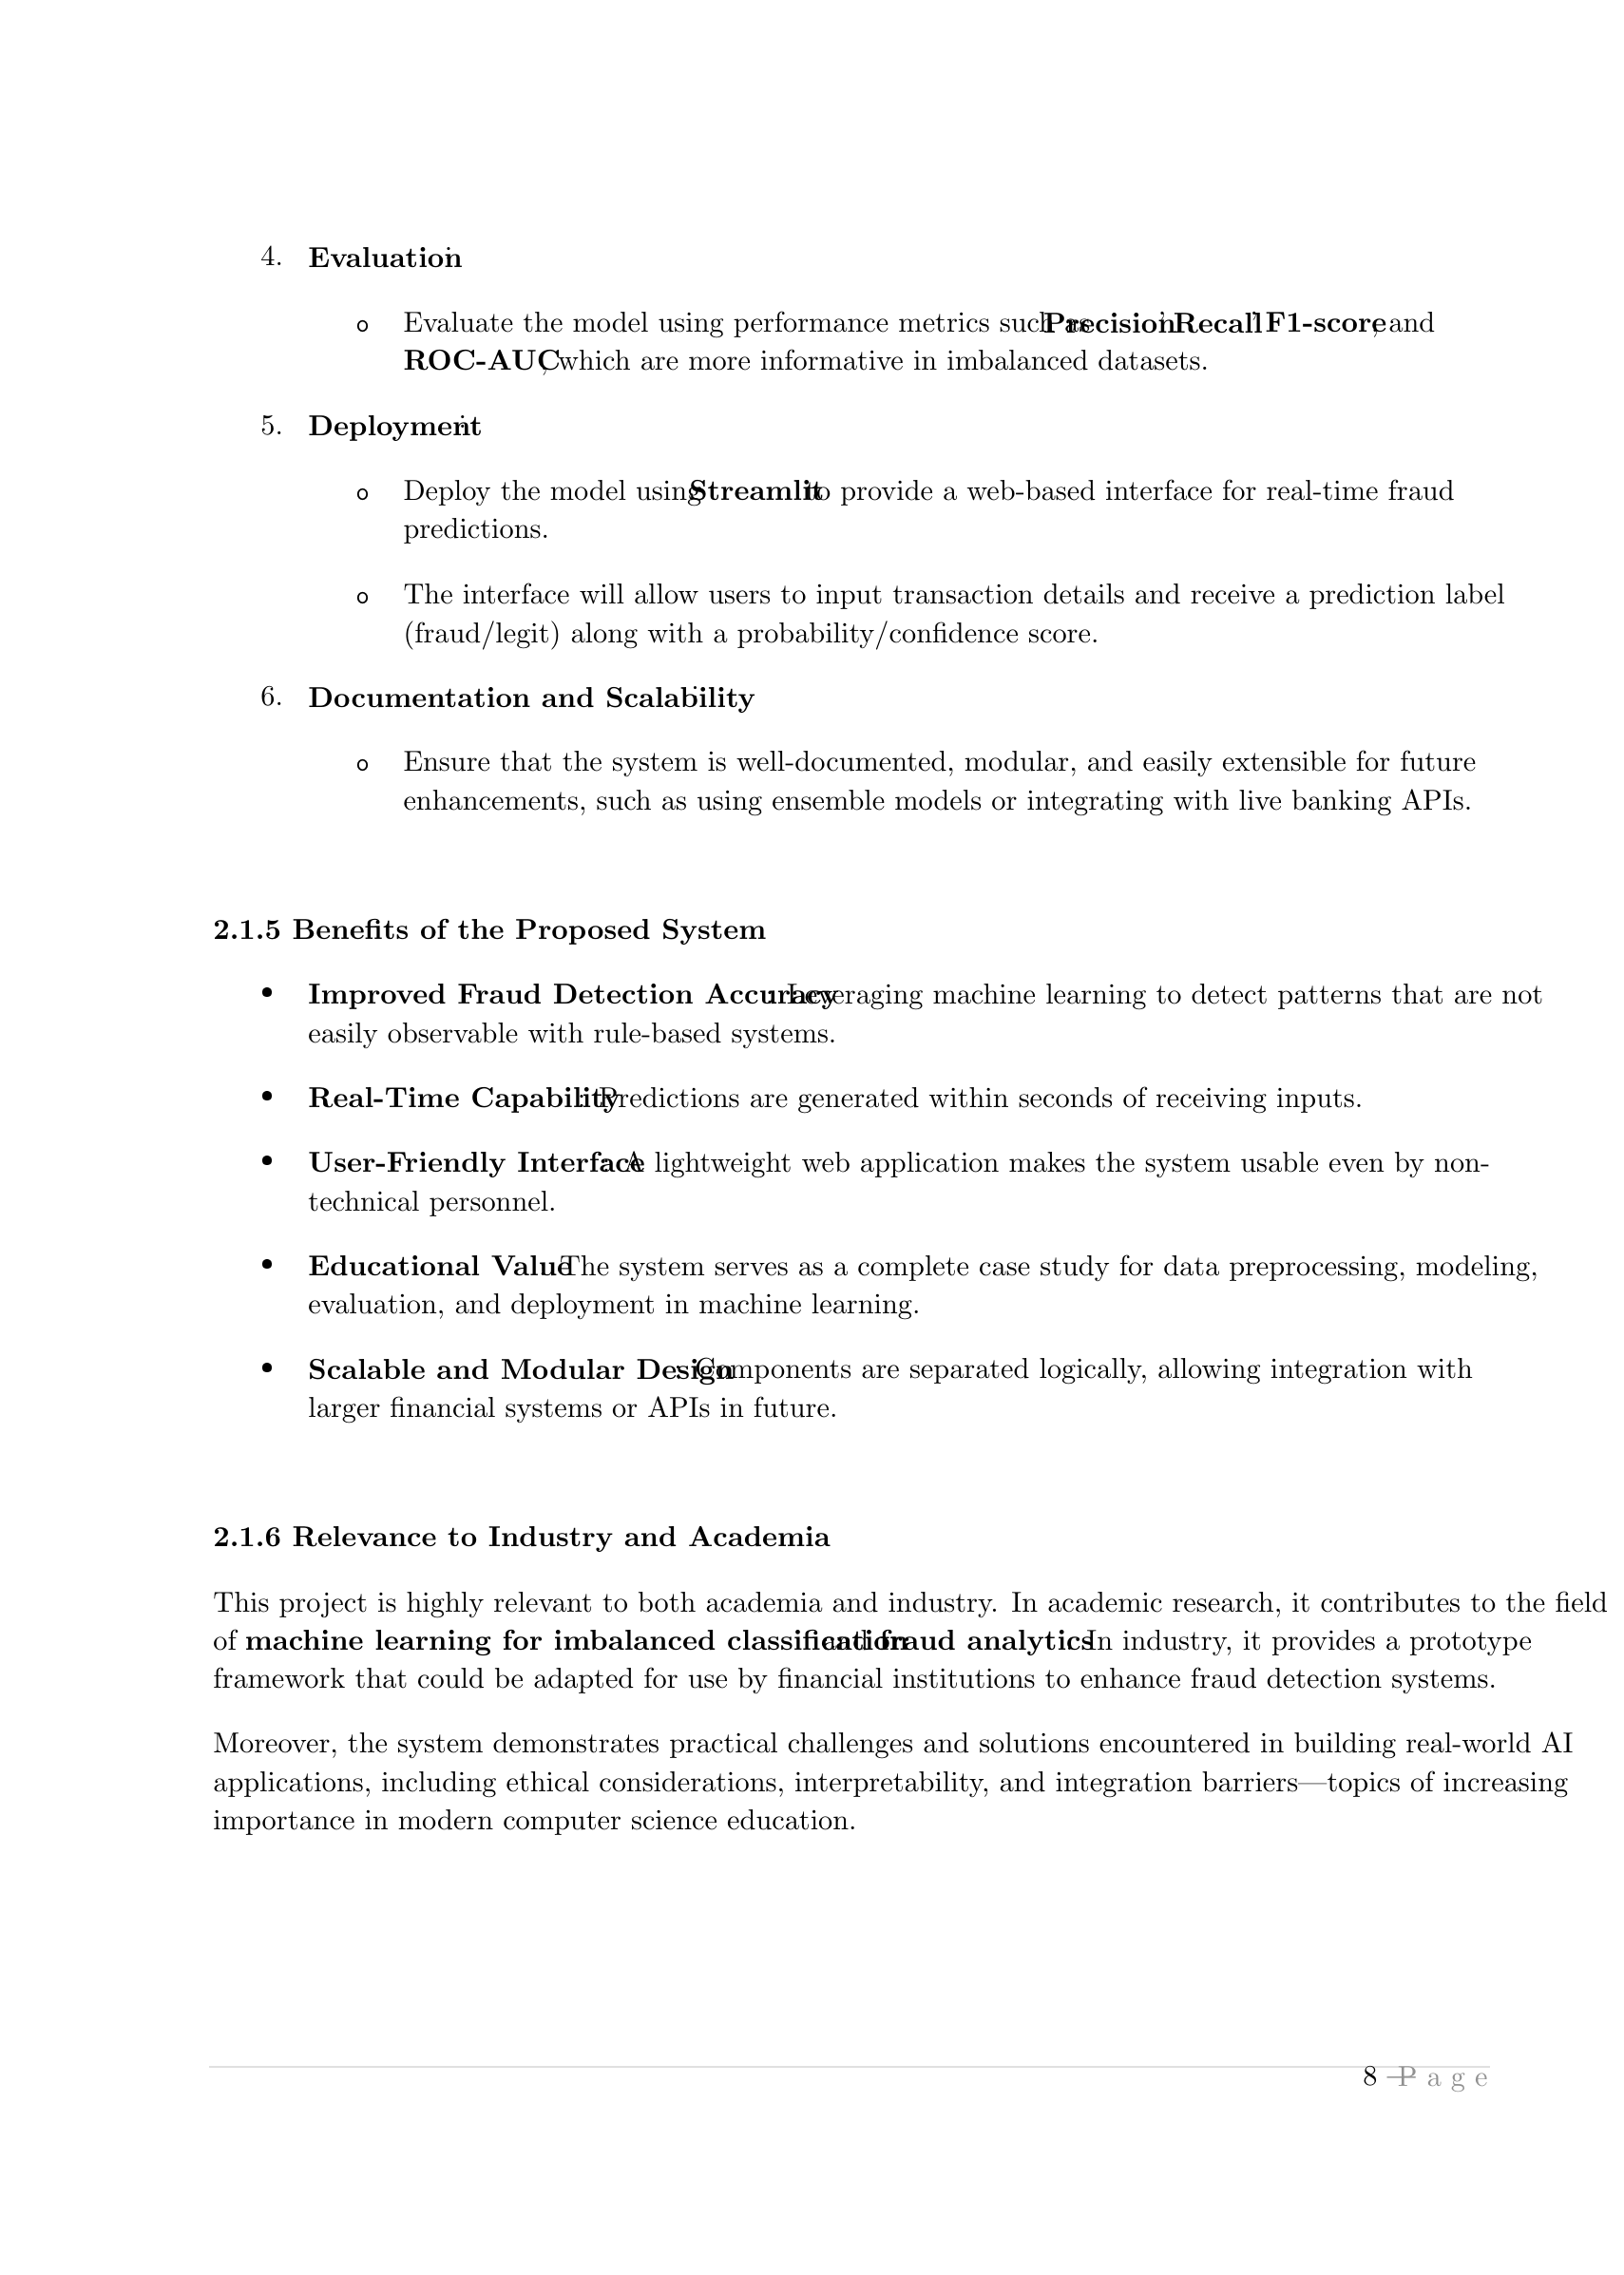
\begin{tikzpicture}[x=1bp,y=-1bp,inner sep=0pt,outer sep=0pt]
  \useasboundingbox (0,0) rectangle (595.20,841.92);
  \fill[fill=pdfcolor9] (69.38,772.78) rectangle (554.40,773.26);
  \node[anchor=north west,inner sep=0pt,outer sep=0pt] at (506.38,772.91) {{\fontsize{11.0bp}{13.2bp}\selectfont 8 | }};
  \node[anchor=north west,inner sep=0pt,outer sep=0pt] at (519.58,772.91) {{\fontsize{11.0bp}{13.2bp}\selectfont \textcolor{pdfcolor1}{P a g e}}};
  \node[anchor=north west,inner sep=0pt,outer sep=0pt] at (550.14,772.91) {{\fontsize{11.0bp}{13.2bp}\selectfont   }};
  \node[anchor=north west,inner sep=0pt,outer sep=0pt] at (88.85,83.67) {{\fontsize{11.0bp}{13.2bp}\selectfont 4.}};
  \node[anchor=north west,inner sep=0pt,outer sep=0pt] at (97.01,83.43) {\textsf{{\fontsize{11.0bp}{13.2bp}\selectfont  }}};
  \node[anchor=north west,inner sep=0pt,outer sep=0pt] at (106.85,83.77) {{\fontsize{11.0bp}{13.2bp}\selectfont \textbf{Evaluation}}};
  \node[anchor=north west,inner sep=0pt,outer sep=0pt] at (158.47,83.67) {{\fontsize{11.0bp}{13.2bp}\selectfont : }};
  \node[anchor=north west,inner sep=0pt,outer sep=0pt] at (124.85,111.63) {\texttt{{\fontsize{10.1bp}{12.1bp}\selectfont o}}};
  \node[anchor=north west,inner sep=0pt,outer sep=0pt] at (130.85,109.18) {\textsf{{\fontsize{10.1bp}{12.1bp}\selectfont  }}};
  \node[anchor=north west,inner sep=0pt,outer sep=0pt] at (142.87,108.39) {{\fontsize{11.0bp}{13.2bp}\selectfont Evaluate the model using performance metrics such as }};
  \node[anchor=north west,inner sep=0pt,outer sep=0pt] at (385.37,108.49) {{\fontsize{11.0bp}{13.2bp}\selectfont \textbf{Precision}}};
  \node[anchor=north west,inner sep=0pt,outer sep=0pt] at (428.83,108.39) {{\fontsize{11.0bp}{13.2bp}\selectfont , }};
  \node[anchor=north west,inner sep=0pt,outer sep=0pt] at (434.59,108.49) {{\fontsize{11.0bp}{13.2bp}\selectfont \textbf{Recall}}};
  \node[anchor=north west,inner sep=0pt,outer sep=0pt] at (463.63,108.39) {{\fontsize{11.0bp}{13.2bp}\selectfont , }};
  \node[anchor=north west,inner sep=0pt,outer sep=0pt] at (469.39,108.49) {{\fontsize{11.0bp}{13.2bp}\selectfont \textbf{F1-score}}};
  \node[anchor=north west,inner sep=0pt,outer sep=0pt] at (509.50,108.39) {{\fontsize{11.0bp}{13.2bp}\selectfont , and }};
  \node[anchor=north west,inner sep=0pt,outer sep=0pt] at (142.87,122.92) {{\fontsize{11.0bp}{13.2bp}\selectfont \textbf{ROC-AUC}}};
  \node[anchor=north west,inner sep=0pt,outer sep=0pt] at (194.71,122.82) {{\fontsize{11.0bp}{13.2bp}\selectfont , which are more informative in imbalanced datasets. }};
  \node[anchor=north west,inner sep=0pt,outer sep=0pt] at (88.85,147.54) {{\fontsize{11.0bp}{13.2bp}\selectfont 5.}};
  \node[anchor=north west,inner sep=0pt,outer sep=0pt] at (97.01,147.30) {\textsf{{\fontsize{11.0bp}{13.2bp}\selectfont  }}};
  \node[anchor=north west,inner sep=0pt,outer sep=0pt] at (106.85,147.64) {{\fontsize{11.0bp}{13.2bp}\selectfont \textbf{Deployment}}};
  \node[anchor=north west,inner sep=0pt,outer sep=0pt] at (163.75,147.54) {{\fontsize{11.0bp}{13.2bp}\selectfont : }};
  \node[anchor=north west,inner sep=0pt,outer sep=0pt] at (124.85,175.26) {\texttt{{\fontsize{10.1bp}{12.1bp}\selectfont o}}};
  \node[anchor=north west,inner sep=0pt,outer sep=0pt] at (130.85,172.81) {\textsf{{\fontsize{10.1bp}{12.1bp}\selectfont  }}};
  \node[anchor=north west,inner sep=0pt,outer sep=0pt] at (142.87,172.02) {{\fontsize{11.0bp}{13.2bp}\selectfont Deploy the model using }};
  \node[anchor=north west,inner sep=0pt,outer sep=0pt] at (251.14,172.12) {{\fontsize{11.0bp}{13.2bp}\selectfont \textbf{Streamlit}}};
  \node[anchor=north west,inner sep=0pt,outer sep=0pt] at (295.08,172.02) {{\fontsize{11.0bp}{13.2bp}\selectfont  to provide a web-based interface for real-time fraud }};
  \node[anchor=north west,inner sep=0pt,outer sep=0pt] at (142.87,186.42) {{\fontsize{11.0bp}{13.2bp}\selectfont predictions. }};
  \node[anchor=north west,inner sep=0pt,outer sep=0pt] at (124.85,214.40) {\texttt{{\fontsize{10.1bp}{12.1bp}\selectfont o}}};
  \node[anchor=north west,inner sep=0pt,outer sep=0pt] at (130.85,211.95) {\textsf{{\fontsize{10.1bp}{12.1bp}\selectfont  }}};
  \node[anchor=north west,inner sep=0pt,outer sep=0pt] at (142.87,211.16) {{\fontsize{11.0bp}{13.2bp}\selectfont The interface will allow users to input transaction details and receive a prediction label }};
  \node[anchor=north west,inner sep=0pt,outer sep=0pt] at (142.87,225.56) {{\fontsize{11.0bp}{13.2bp}\selectfont (fraud/legit) along with a probability/confidence score. }};
  \node[anchor=north west,inner sep=0pt,outer sep=0pt] at (88.85,250.28) {{\fontsize{11.0bp}{13.2bp}\selectfont 6.}};
  \node[anchor=north west,inner sep=0pt,outer sep=0pt] at (97.01,250.04) {\textsf{{\fontsize{11.0bp}{13.2bp}\selectfont  }}};
  \node[anchor=north west,inner sep=0pt,outer sep=0pt] at (106.85,250.38) {{\fontsize{11.0bp}{13.2bp}\selectfont \textbf{Documentation and Scalability}}};
  \node[anchor=north west,inner sep=0pt,outer sep=0pt] at (251.86,250.28) {{\fontsize{11.0bp}{13.2bp}\selectfont : }};
  \node[anchor=north west,inner sep=0pt,outer sep=0pt] at (124.85,278.00) {\texttt{{\fontsize{10.1bp}{12.1bp}\selectfont o}}};
  \node[anchor=north west,inner sep=0pt,outer sep=0pt] at (130.85,275.55) {\textsf{{\fontsize{10.1bp}{12.1bp}\selectfont  }}};
  \node[anchor=north west,inner sep=0pt,outer sep=0pt] at (142.87,274.76) {{\fontsize{11.0bp}{13.2bp}\selectfont Ensure that the system is well-documented, modular, and easily extensible for future }};
  \node[anchor=north west,inner sep=0pt,outer sep=0pt] at (142.87,289.19) {{\fontsize{11.0bp}{13.2bp}\selectfont enhancements, such as using ensemble models or integrating with live banking APIs. }};
  \node[anchor=north west,inner sep=0pt,outer sep=0pt] at (70.82,338.49) {{\fontsize{11.0bp}{13.2bp}\selectfont \textbf{2.1.5 Benefits of the Proposed System }}};
  \node[anchor=north west,inner sep=0pt,outer sep=0pt] at (88.85,364.37) {{\fontsize{10.1bp}{12.1bp}\selectfont •}};
  \node[anchor=north west,inner sep=0pt,outer sep=0pt] at (93.41,363.66) {\textsf{{\fontsize{10.1bp}{12.1bp}\selectfont  }}};
  \node[anchor=north west,inner sep=0pt,outer sep=0pt] at (106.85,362.97) {{\fontsize{11.0bp}{13.2bp}\selectfont \textbf{Improved Fraud Detection Accuracy}}};
  \node[anchor=north west,inner sep=0pt,outer sep=0pt] at (280.20,362.87) {{\fontsize{11.0bp}{13.2bp}\selectfont : Leveraging machine learning to detect patterns that are not }};
  \node[anchor=north west,inner sep=0pt,outer sep=0pt] at (106.85,377.53) {{\fontsize{11.0bp}{13.2bp}\selectfont easily observable with rule-based systems. }};
  \node[anchor=north west,inner sep=0pt,outer sep=0pt] at (88.85,403.51) {{\fontsize{10.1bp}{12.1bp}\selectfont •}};
  \node[anchor=north west,inner sep=0pt,outer sep=0pt] at (93.41,402.80) {\textsf{{\fontsize{10.1bp}{12.1bp}\selectfont  }}};
  \node[anchor=north west,inner sep=0pt,outer sep=0pt] at (106.85,402.11) {{\fontsize{11.0bp}{13.2bp}\selectfont \textbf{Real-Time Capability}}};
  \node[anchor=north west,inner sep=0pt,outer sep=0pt] at (208.90,402.01) {{\fontsize{11.0bp}{13.2bp}\selectfont : Predictions are generated within seconds of receiving inputs. }};
  \node[anchor=north west,inner sep=0pt,outer sep=0pt] at (88.85,427.99) {{\fontsize{10.1bp}{12.1bp}\selectfont •}};
  \node[anchor=north west,inner sep=0pt,outer sep=0pt] at (93.41,427.28) {\textsf{{\fontsize{10.1bp}{12.1bp}\selectfont  }}};
  \node[anchor=north west,inner sep=0pt,outer sep=0pt] at (106.85,426.59) {{\fontsize{11.0bp}{13.2bp}\selectfont \textbf{User-Friendly Interface}}};
  \node[anchor=north west,inner sep=0pt,outer sep=0pt] at (218.26,426.49) {{\fontsize{11.0bp}{13.2bp}\selectfont : A lightweight web application makes the system usable even by non-}};
  \node[anchor=north west,inner sep=0pt,outer sep=0pt] at (106.85,441.13) {{\fontsize{11.0bp}{13.2bp}\selectfont technical personnel. }};
  \node[anchor=north west,inner sep=0pt,outer sep=0pt] at (88.85,467.13) {{\fontsize{10.1bp}{12.1bp}\selectfont •}};
  \node[anchor=north west,inner sep=0pt,outer sep=0pt] at (93.41,466.42) {\textsf{{\fontsize{10.1bp}{12.1bp}\selectfont  }}};
  \node[anchor=north west,inner sep=0pt,outer sep=0pt] at (106.85,465.73) {{\fontsize{11.0bp}{13.2bp}\selectfont \textbf{Educational Value}}};
  \node[anchor=north west,inner sep=0pt,outer sep=0pt] at (194.23,465.63) {{\fontsize{11.0bp}{13.2bp}\selectfont : The system serves as a complete case study for data preprocessing, modeling, }};
  \node[anchor=north west,inner sep=0pt,outer sep=0pt] at (106.85,480.27) {{\fontsize{11.0bp}{13.2bp}\selectfont evaluation, and deployment in machine learning. }};
  \node[anchor=north west,inner sep=0pt,outer sep=0pt] at (88.85,506.25) {{\fontsize{10.1bp}{12.1bp}\selectfont •}};
  \node[anchor=north west,inner sep=0pt,outer sep=0pt] at (93.41,505.54) {\textsf{{\fontsize{10.1bp}{12.1bp}\selectfont  }}};
  \node[anchor=north west,inner sep=0pt,outer sep=0pt] at (106.85,504.85) {{\fontsize{11.0bp}{13.2bp}\selectfont \textbf{Scalable and Modular Design}}};
  \node[anchor=north west,inner sep=0pt,outer sep=0pt] at (245.38,504.75) {{\fontsize{11.0bp}{13.2bp}\selectfont : Components are separated logically, allowing integration with }};
  \node[anchor=north west,inner sep=0pt,outer sep=0pt] at (106.85,519.39) {{\fontsize{11.0bp}{13.2bp}\selectfont larger financial systems or APIs in future. }};
  \node[anchor=north west,inner sep=0pt,outer sep=0pt] at (70.82,568.48) {{\fontsize{11.0bp}{13.2bp}\selectfont \textbf{2.1.6 Relevance to Industry and Academia }}};
  \node[anchor=north west,inner sep=0pt,outer sep=0pt] at (70.82,593.10) {{\fontsize{11.0bp}{13.2bp}\selectfont This project is highly relevant to both academia and industry. In academic research, it contributes to the field }};
  \node[anchor=north west,inner sep=0pt,outer sep=0pt] at (70.82,607.50) {{\fontsize{11.0bp}{13.2bp}\selectfont of }};
  \node[anchor=north west,inner sep=0pt,outer sep=0pt] at (82.85,607.60) {{\fontsize{11.0bp}{13.2bp}\selectfont \textbf{machine learning for imbalanced classification}}};
  \node[anchor=north west,inner sep=0pt,outer sep=0pt] at (301.56,607.50) {{\fontsize{11.0bp}{13.2bp}\selectfont  and }};
  \node[anchor=north west,inner sep=0pt,outer sep=0pt] at (323.18,607.60) {{\fontsize{11.0bp}{13.2bp}\selectfont \textbf{fraud analytics}}};
  \node[anchor=north west,inner sep=0pt,outer sep=0pt] at (393.77,607.50) {{\fontsize{11.0bp}{13.2bp}\selectfont . In industry, it provides a prototype }};
  \node[anchor=north west,inner sep=0pt,outer sep=0pt] at (70.82,622.14) {{\fontsize{11.0bp}{13.2bp}\selectfont framework that could be adapted for use by financial institutions to enhance fraud detection systems. }};
  \node[anchor=north west,inner sep=0pt,outer sep=0pt] at (70.82,646.64) {{\fontsize{11.0bp}{13.2bp}\selectfont Moreover, the system demonstrates practical challenges and solutions encountered in building real-world AI }};
  \node[anchor=north west,inner sep=0pt,outer sep=0pt] at (70.82,661.28) {{\fontsize{11.0bp}{13.2bp}\selectfont applications, including ethical considerations, interpretability, and integration barriers---topics of increasing }};
  \node[anchor=north west,inner sep=0pt,outer sep=0pt] at (70.82,675.68) {{\fontsize{11.0bp}{13.2bp}\selectfont importance in modern computer science education. }};
\end{tikzpicture}
\newpage
\noindent

\begin{tikzpicture}[x=1bp,y=-1bp,inner sep=0pt,outer sep=0pt]
  \useasboundingbox (0,0) rectangle (595.20,841.92);
  \fill[fill=pdfcolor9] (69.38,772.78) rectangle (554.40,773.26);
  \fill[fill=black] (142.87,124.10) rectangle (492.69,125.54);
  \node[anchor=north west,inner sep=0pt,outer sep=0pt] at (506.38,772.91) {{\fontsize{11.0bp}{13.2bp}\selectfont 9 | }};
  \node[anchor=north west,inner sep=0pt,outer sep=0pt] at (519.58,772.91) {{\fontsize{11.0bp}{13.2bp}\selectfont \textcolor{pdfcolor1}{P a g e}}};
  \node[anchor=north west,inner sep=0pt,outer sep=0pt] at (550.14,772.91) {{\fontsize{11.0bp}{13.2bp}\selectfont   }};
  \node[anchor=north west,inner sep=0pt,outer sep=0pt] at (142.87,108.13) {{\fontsize{13.9bp}{16.7bp}\selectfont \textbf{2.2 REQUIREMENT ANALYSIS AND DEVELOPMENT }}};
  \node[anchor=north west,inner sep=0pt,outer sep=0pt] at (70.82,142.50) {{\fontsize{11.0bp}{13.2bp}\selectfont This section outlines the software requirements critical for the successful implementation of the Credit Card }};
  \node[anchor=north west,inner sep=0pt,outer sep=0pt] at (70.82,157.14) {{\fontsize{11.0bp}{13.2bp}\selectfont Fraud Detection System. The requirements are divided into two categories---Functional and Non-}};
  \node[anchor=north west,inner sep=0pt,outer sep=0pt] at (70.82,171.54) {{\fontsize{11.0bp}{13.2bp}\selectfont Functional---and are followed by the Goals of Implementation, each expanded to provide a comprehensive }};
  \node[anchor=north west,inner sep=0pt,outer sep=0pt] at (70.82,186.18) {{\fontsize{11.0bp}{13.2bp}\selectfont understanding of the system expectations. }};
  \node[anchor=north west,inner sep=0pt,outer sep=0pt] at (70.82,235.26) {{\fontsize{11.0bp}{13.2bp}\selectfont \textbf{2.2.1 Functional Requirements }}};
  \node[anchor=north west,inner sep=0pt,outer sep=0pt] at (70.82,259.88) {{\fontsize{11.0bp}{13.2bp}\selectfont Functional requirements define the specific behavior and functions the system must perform to fulfill its }};
  \node[anchor=north west,inner sep=0pt,outer sep=0pt] at (70.82,274.28) {{\fontsize{11.0bp}{13.2bp}\selectfont objectives. For this project, the functional requirements focus on the core capabilities of the fraud detection }};
  \node[anchor=north west,inner sep=0pt,outer sep=0pt] at (70.82,288.95) {{\fontsize{11.0bp}{13.2bp}\selectfont system, from data processing and model training to prediction and UI interaction. }};
  \node[anchor=north west,inner sep=0pt,outer sep=0pt] at (70.82,313.53) {{\fontsize{11.0bp}{13.2bp}\selectfont \textbf{2.2.1.1 Data Loading and Preprocessing }}};
  \node[anchor=north west,inner sep=0pt,outer sep=0pt] at (88.85,339.41) {{\fontsize{10.1bp}{12.1bp}\selectfont •}};
  \node[anchor=north west,inner sep=0pt,outer sep=0pt] at (93.41,338.70) {\textsf{{\fontsize{10.1bp}{12.1bp}\selectfont  }}};
  \node[anchor=north west,inner sep=0pt,outer sep=0pt] at (106.85,337.91) {{\fontsize{11.0bp}{13.2bp}\selectfont The system shall load transaction data from a .csv file. }};
  \node[anchor=north west,inner sep=0pt,outer sep=0pt] at (88.85,364.13) {{\fontsize{10.1bp}{12.1bp}\selectfont •}};
  \node[anchor=north west,inner sep=0pt,outer sep=0pt] at (93.41,363.42) {\textsf{{\fontsize{10.1bp}{12.1bp}\selectfont  }}};
  \node[anchor=north west,inner sep=0pt,outer sep=0pt] at (106.85,362.63) {{\fontsize{11.0bp}{13.2bp}\selectfont The system shall normalize continuous variables (e.g., Time and Amount). }};
  \node[anchor=north west,inner sep=0pt,outer sep=0pt] at (88.85,388.63) {{\fontsize{10.1bp}{12.1bp}\selectfont •}};
  \node[anchor=north west,inner sep=0pt,outer sep=0pt] at (93.41,387.92) {\textsf{{\fontsize{10.1bp}{12.1bp}\selectfont  }}};
  \node[anchor=north west,inner sep=0pt,outer sep=0pt] at (106.85,387.13) {{\fontsize{11.0bp}{13.2bp}\selectfont The system shall handle missing values (if any) appropriately. }};
  \node[anchor=north west,inner sep=0pt,outer sep=0pt] at (88.85,413.11) {{\fontsize{10.1bp}{12.1bp}\selectfont •}};
  \node[anchor=north west,inner sep=0pt,outer sep=0pt] at (93.41,412.40) {\textsf{{\fontsize{10.1bp}{12.1bp}\selectfont  }}};
  \node[anchor=north west,inner sep=0pt,outer sep=0pt] at (106.85,411.61) {{\fontsize{11.0bp}{13.2bp}\selectfont The system shall apply SMOTE to balance the class distribution. }};
  \node[anchor=north west,inner sep=0pt,outer sep=0pt] at (70.82,436.19) {{\fontsize{11.0bp}{13.2bp}\selectfont \textbf{2.2.1.2 Model Training }}};
  \node[anchor=north west,inner sep=0pt,outer sep=0pt] at (88.85,462.33) {{\fontsize{10.1bp}{12.1bp}\selectfont •}};
  \node[anchor=north west,inner sep=0pt,outer sep=0pt] at (93.41,461.62) {\textsf{{\fontsize{10.1bp}{12.1bp}\selectfont  }}};
  \node[anchor=north west,inner sep=0pt,outer sep=0pt] at (106.85,460.83) {{\fontsize{11.0bp}{13.2bp}\selectfont The system shall allow training of a machine learning model (Random Forest). }};
  \node[anchor=north west,inner sep=0pt,outer sep=0pt] at (88.85,486.81) {{\fontsize{10.1bp}{12.1bp}\selectfont •}};
  \node[anchor=north west,inner sep=0pt,outer sep=0pt] at (93.41,486.10) {\textsf{{\fontsize{10.1bp}{12.1bp}\selectfont  }}};
  \node[anchor=north west,inner sep=0pt,outer sep=0pt] at (106.85,485.31) {{\fontsize{11.0bp}{13.2bp}\selectfont The system shall split the data into training and testing subsets. }};
  \node[anchor=north west,inner sep=0pt,outer sep=0pt] at (88.85,511.29) {{\fontsize{10.1bp}{12.1bp}\selectfont •}};
  \node[anchor=north west,inner sep=0pt,outer sep=0pt] at (93.41,510.58) {\textsf{{\fontsize{10.1bp}{12.1bp}\selectfont  }}};
  \node[anchor=north west,inner sep=0pt,outer sep=0pt] at (106.85,509.79) {{\fontsize{11.0bp}{13.2bp}\selectfont The system shall store the trained model using joblib for reuse. }};
  \node[anchor=north west,inner sep=0pt,outer sep=0pt] at (70.82,534.61) {{\fontsize{11.0bp}{13.2bp}\selectfont \textbf{2.2.1.3 Evaluation }}};
  \node[anchor=north west,inner sep=0pt,outer sep=0pt] at (88.85,560.52) {{\fontsize{10.1bp}{12.1bp}\selectfont •}};
  \node[anchor=north west,inner sep=0pt,outer sep=0pt] at (93.41,559.81) {\textsf{{\fontsize{10.1bp}{12.1bp}\selectfont  }}};
  \node[anchor=north west,inner sep=0pt,outer sep=0pt] at (106.85,559.02) {{\fontsize{11.0bp}{13.2bp}\selectfont The system shall generate performance metrics: Accuracy, Precision, Recall, F1-Score, and ROC-}};
  \node[anchor=north west,inner sep=0pt,outer sep=0pt] at (106.85,573.42) {{\fontsize{11.0bp}{13.2bp}\selectfont AUC. }};
  \node[anchor=north west,inner sep=0pt,outer sep=0pt] at (88.85,599.64) {{\fontsize{10.1bp}{12.1bp}\selectfont •}};
  \node[anchor=north west,inner sep=0pt,outer sep=0pt] at (93.41,598.93) {\textsf{{\fontsize{10.1bp}{12.1bp}\selectfont  }}};
  \node[anchor=north west,inner sep=0pt,outer sep=0pt] at (106.85,598.14) {{\fontsize{11.0bp}{13.2bp}\selectfont The system shall display a confusion matrix and ROC curve. }};
  \node[anchor=north west,inner sep=0pt,outer sep=0pt] at (88.85,624.12) {{\fontsize{10.1bp}{12.1bp}\selectfont •}};
  \node[anchor=north west,inner sep=0pt,outer sep=0pt] at (93.41,623.41) {\textsf{{\fontsize{10.1bp}{12.1bp}\selectfont  }}};
  \node[anchor=north west,inner sep=0pt,outer sep=0pt] at (106.85,622.62) {{\fontsize{11.0bp}{13.2bp}\selectfont The system shall log evaluation results for further review. }};
  \node[anchor=north west,inner sep=0pt,outer sep=0pt] at (70.82,647.22) {{\fontsize{11.0bp}{13.2bp}\selectfont \textbf{2.2.1.4 Prediction Module }}};
  \node[anchor=north west,inner sep=0pt,outer sep=0pt] at (88.85,673.34) {{\fontsize{10.1bp}{12.1bp}\selectfont •}};
  \node[anchor=north west,inner sep=0pt,outer sep=0pt] at (93.41,672.63) {\textsf{{\fontsize{10.1bp}{12.1bp}\selectfont  }}};
  \node[anchor=north west,inner sep=0pt,outer sep=0pt] at (106.85,671.84) {{\fontsize{11.0bp}{13.2bp}\selectfont The system shall accept a set of features (V1-V28, Time, Amount) as input. }};
  \node[anchor=north west,inner sep=0pt,outer sep=0pt] at (88.85,697.82) {{\fontsize{10.1bp}{12.1bp}\selectfont •}};
  \node[anchor=north west,inner sep=0pt,outer sep=0pt] at (93.41,697.11) {\textsf{{\fontsize{10.1bp}{12.1bp}\selectfont  }}};
  \node[anchor=north west,inner sep=0pt,outer sep=0pt] at (106.85,696.32) {{\fontsize{11.0bp}{13.2bp}\selectfont The system shall use the trained model to return a binary classification: 0 (Legit) or 1 (Fraud). }};
  \node[anchor=north west,inner sep=0pt,outer sep=0pt] at (88.85,722.33) {{\fontsize{10.1bp}{12.1bp}\selectfont •}};
  \node[anchor=north west,inner sep=0pt,outer sep=0pt] at (93.41,721.62) {\textsf{{\fontsize{10.1bp}{12.1bp}\selectfont  }}};
  \node[anchor=north west,inner sep=0pt,outer sep=0pt] at (106.85,720.83) {{\fontsize{11.0bp}{13.2bp}\selectfont The system shall return the probability (confidence score) associated with each prediction. }};
  \node[anchor=north west,inner sep=0pt,outer sep=0pt] at (70.82,745.41) {{\fontsize{11.0bp}{13.2bp}\selectfont \textbf{2.2.1.5 User Interface (UI) }}};
\end{tikzpicture}
\newpage
\noindent
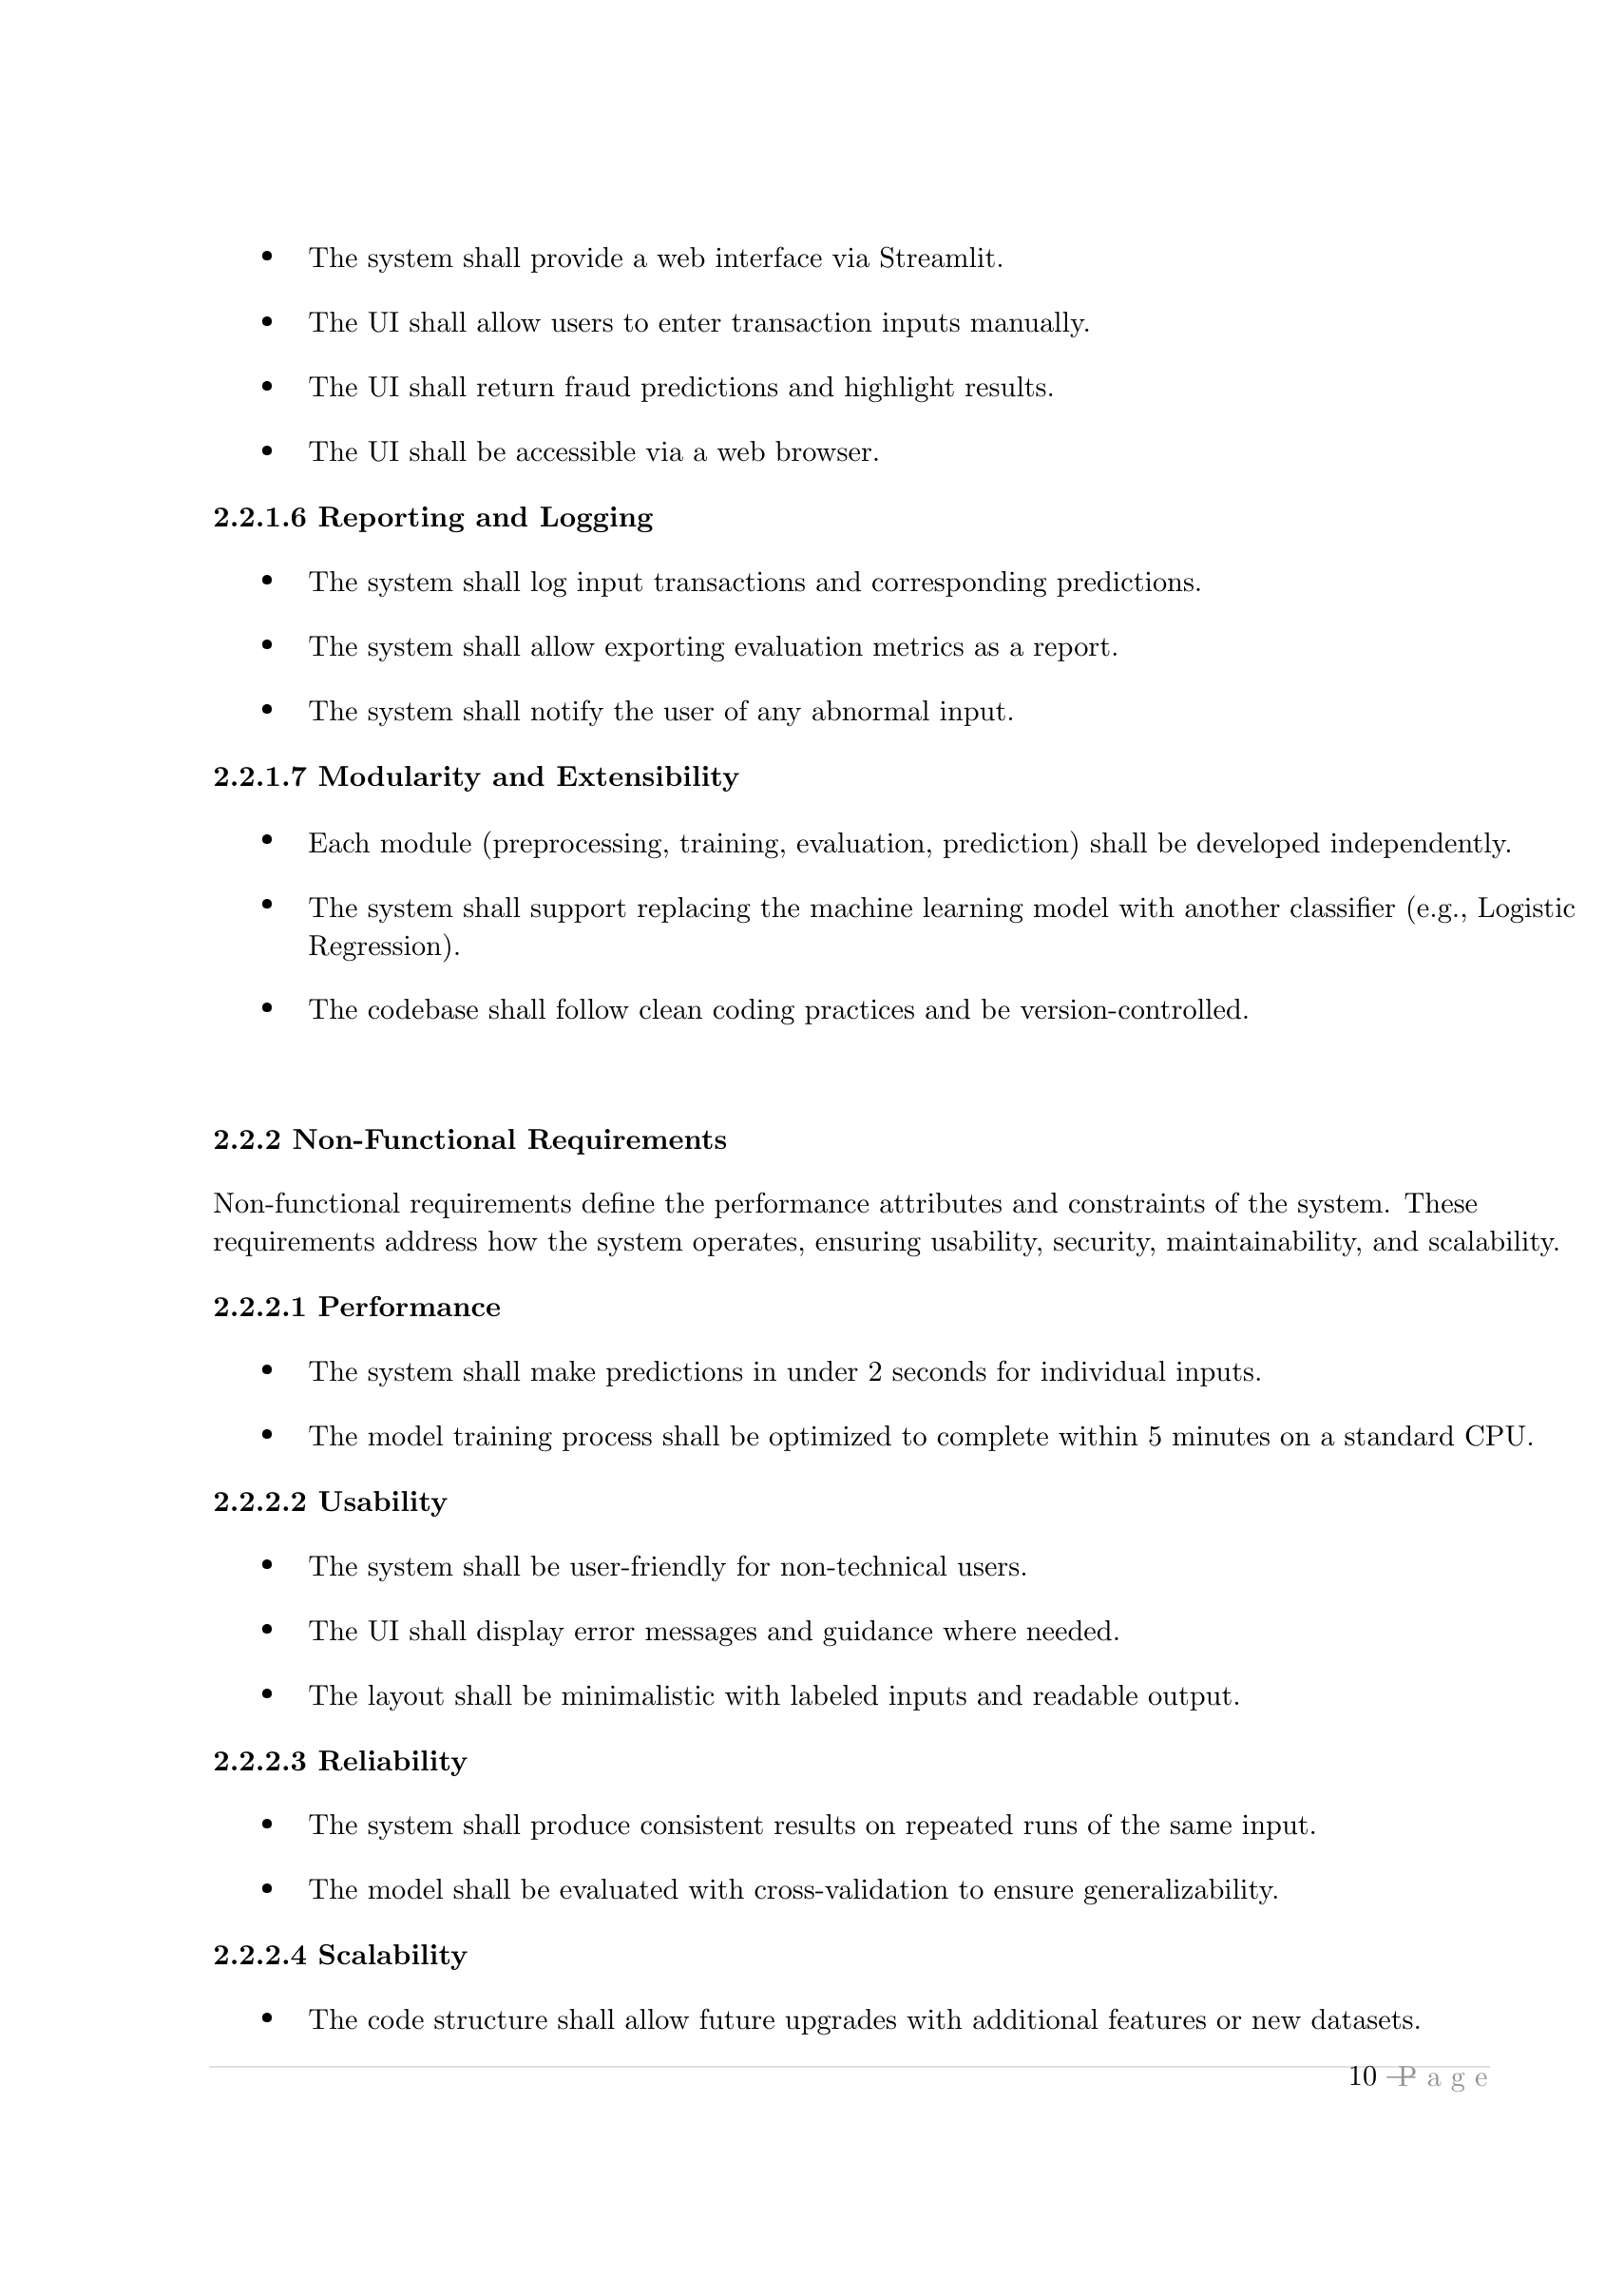
\begin{tikzpicture}[x=1bp,y=-1bp,inner sep=0pt,outer sep=0pt]
  \useasboundingbox (0,0) rectangle (595.20,841.92);
  \fill[fill=pdfcolor9] (69.38,772.78) rectangle (554.40,773.26);
  \node[anchor=north west,inner sep=0pt,outer sep=0pt] at (500.86,772.91) {{\fontsize{11.0bp}{13.2bp}\selectfont 10 | }};
  \node[anchor=north west,inner sep=0pt,outer sep=0pt] at (519.58,772.91) {{\fontsize{11.0bp}{13.2bp}\selectfont \textcolor{pdfcolor1}{P a g e}}};
  \node[anchor=north west,inner sep=0pt,outer sep=0pt] at (550.14,772.91) {{\fontsize{11.0bp}{13.2bp}\selectfont   }};
  \node[anchor=north west,inner sep=0pt,outer sep=0pt] at (88.85,85.17) {{\fontsize{10.1bp}{12.1bp}\selectfont •}};
  \node[anchor=north west,inner sep=0pt,outer sep=0pt] at (93.41,84.46) {\textsf{{\fontsize{10.1bp}{12.1bp}\selectfont  }}};
  \node[anchor=north west,inner sep=0pt,outer sep=0pt] at (106.85,83.67) {{\fontsize{11.0bp}{13.2bp}\selectfont The system shall provide a web interface via Streamlit. }};
  \node[anchor=north west,inner sep=0pt,outer sep=0pt] at (88.85,109.89) {{\fontsize{10.1bp}{12.1bp}\selectfont •}};
  \node[anchor=north west,inner sep=0pt,outer sep=0pt] at (93.41,109.18) {\textsf{{\fontsize{10.1bp}{12.1bp}\selectfont  }}};
  \node[anchor=north west,inner sep=0pt,outer sep=0pt] at (106.85,108.39) {{\fontsize{11.0bp}{13.2bp}\selectfont The UI shall allow users to enter transaction inputs manually. }};
  \node[anchor=north west,inner sep=0pt,outer sep=0pt] at (88.85,134.40) {{\fontsize{10.1bp}{12.1bp}\selectfont •}};
  \node[anchor=north west,inner sep=0pt,outer sep=0pt] at (93.41,133.69) {\textsf{{\fontsize{10.1bp}{12.1bp}\selectfont  }}};
  \node[anchor=north west,inner sep=0pt,outer sep=0pt] at (106.85,132.90) {{\fontsize{11.0bp}{13.2bp}\selectfont The UI shall return fraud predictions and highlight results. }};
  \node[anchor=north west,inner sep=0pt,outer sep=0pt] at (88.85,158.88) {{\fontsize{10.1bp}{12.1bp}\selectfont •}};
  \node[anchor=north west,inner sep=0pt,outer sep=0pt] at (93.41,158.17) {\textsf{{\fontsize{10.1bp}{12.1bp}\selectfont  }}};
  \node[anchor=north west,inner sep=0pt,outer sep=0pt] at (106.85,157.38) {{\fontsize{11.0bp}{13.2bp}\selectfont The UI shall be accessible via a web browser. }};
  \node[anchor=north west,inner sep=0pt,outer sep=0pt] at (70.82,181.96) {{\fontsize{11.0bp}{13.2bp}\selectfont \textbf{2.2.1.6 Reporting and Logging }}};
  \node[anchor=north west,inner sep=0pt,outer sep=0pt] at (88.85,208.10) {{\fontsize{10.1bp}{12.1bp}\selectfont •}};
  \node[anchor=north west,inner sep=0pt,outer sep=0pt] at (93.41,207.39) {\textsf{{\fontsize{10.1bp}{12.1bp}\selectfont  }}};
  \node[anchor=north west,inner sep=0pt,outer sep=0pt] at (106.85,206.60) {{\fontsize{11.0bp}{13.2bp}\selectfont The system shall log input transactions and corresponding predictions. }};
  \node[anchor=north west,inner sep=0pt,outer sep=0pt] at (88.85,232.58) {{\fontsize{10.1bp}{12.1bp}\selectfont •}};
  \node[anchor=north west,inner sep=0pt,outer sep=0pt] at (93.41,231.87) {\textsf{{\fontsize{10.1bp}{12.1bp}\selectfont  }}};
  \node[anchor=north west,inner sep=0pt,outer sep=0pt] at (106.85,231.08) {{\fontsize{11.0bp}{13.2bp}\selectfont The system shall allow exporting evaluation metrics as a report. }};
  \node[anchor=north west,inner sep=0pt,outer sep=0pt] at (88.85,257.06) {{\fontsize{10.1bp}{12.1bp}\selectfont •}};
  \node[anchor=north west,inner sep=0pt,outer sep=0pt] at (93.41,256.35) {\textsf{{\fontsize{10.1bp}{12.1bp}\selectfont  }}};
  \node[anchor=north west,inner sep=0pt,outer sep=0pt] at (106.85,255.56) {{\fontsize{11.0bp}{13.2bp}\selectfont The system shall notify the user of any abnormal input. }};
  \node[anchor=north west,inner sep=0pt,outer sep=0pt] at (70.82,280.38) {{\fontsize{11.0bp}{13.2bp}\selectfont \textbf{2.2.1.7 Modularity and Extensibility }}};
  \node[anchor=north west,inner sep=0pt,outer sep=0pt] at (88.85,306.29) {{\fontsize{10.1bp}{12.1bp}\selectfont •}};
  \node[anchor=north west,inner sep=0pt,outer sep=0pt] at (93.41,305.58) {\textsf{{\fontsize{10.1bp}{12.1bp}\selectfont  }}};
  \node[anchor=north west,inner sep=0pt,outer sep=0pt] at (106.85,304.79) {{\fontsize{11.0bp}{13.2bp}\selectfont Each module (preprocessing, training, evaluation, prediction) shall be developed independently. }};
  \node[anchor=north west,inner sep=0pt,outer sep=0pt] at (88.85,330.77) {{\fontsize{10.1bp}{12.1bp}\selectfont •}};
  \node[anchor=north west,inner sep=0pt,outer sep=0pt] at (93.41,330.06) {\textsf{{\fontsize{10.1bp}{12.1bp}\selectfont  }}};
  \node[anchor=north west,inner sep=0pt,outer sep=0pt] at (106.85,329.27) {{\fontsize{11.0bp}{13.2bp}\selectfont The system shall support replacing the machine learning model with another classifier (e.g., Logistic }};
  \node[anchor=north west,inner sep=0pt,outer sep=0pt] at (106.85,343.91) {{\fontsize{11.0bp}{13.2bp}\selectfont Regression). }};
  \node[anchor=north west,inner sep=0pt,outer sep=0pt] at (88.85,369.89) {{\fontsize{10.1bp}{12.1bp}\selectfont •}};
  \node[anchor=north west,inner sep=0pt,outer sep=0pt] at (93.41,369.18) {\textsf{{\fontsize{10.1bp}{12.1bp}\selectfont  }}};
  \node[anchor=north west,inner sep=0pt,outer sep=0pt] at (106.85,368.39) {{\fontsize{11.0bp}{13.2bp}\selectfont The codebase shall follow clean coding practices and be version-controlled. }};
  \node[anchor=north west,inner sep=0pt,outer sep=0pt] at (70.82,417.71) {{\fontsize{11.0bp}{13.2bp}\selectfont \textbf{2.2.2 Non-Functional Requirements }}};
  \node[anchor=north west,inner sep=0pt,outer sep=0pt] at (70.82,442.09) {{\fontsize{11.0bp}{13.2bp}\selectfont Non-functional requirements define the performance attributes and constraints of the system. These }};
  \node[anchor=north west,inner sep=0pt,outer sep=0pt] at (70.82,456.49) {{\fontsize{11.0bp}{13.2bp}\selectfont requirements address how the system operates, ensuring usability, security, maintainability, and scalability. }};
  \node[anchor=north west,inner sep=0pt,outer sep=0pt] at (70.82,481.33) {{\fontsize{11.0bp}{13.2bp}\selectfont \textbf{2.2.2.1 Performance }}};
  \node[anchor=north west,inner sep=0pt,outer sep=0pt] at (88.85,507.21) {{\fontsize{10.1bp}{12.1bp}\selectfont •}};
  \node[anchor=north west,inner sep=0pt,outer sep=0pt] at (93.41,506.50) {\textsf{{\fontsize{10.1bp}{12.1bp}\selectfont  }}};
  \node[anchor=north west,inner sep=0pt,outer sep=0pt] at (106.85,505.71) {{\fontsize{11.0bp}{13.2bp}\selectfont The system shall make predictions in under 2 seconds for individual inputs. }};
  \node[anchor=north west,inner sep=0pt,outer sep=0pt] at (88.85,531.69) {{\fontsize{10.1bp}{12.1bp}\selectfont •}};
  \node[anchor=north west,inner sep=0pt,outer sep=0pt] at (93.41,530.98) {\textsf{{\fontsize{10.1bp}{12.1bp}\selectfont  }}};
  \node[anchor=north west,inner sep=0pt,outer sep=0pt] at (106.85,530.19) {{\fontsize{11.0bp}{13.2bp}\selectfont The model training process shall be optimized to complete within 5 minutes on a standard CPU. }};
  \node[anchor=north west,inner sep=0pt,outer sep=0pt] at (70.82,555.04) {{\fontsize{11.0bp}{13.2bp}\selectfont \textbf{2.2.2.2 Usability }}};
  \node[anchor=north west,inner sep=0pt,outer sep=0pt] at (88.85,580.92) {{\fontsize{10.1bp}{12.1bp}\selectfont •}};
  \node[anchor=north west,inner sep=0pt,outer sep=0pt] at (93.41,580.21) {\textsf{{\fontsize{10.1bp}{12.1bp}\selectfont  }}};
  \node[anchor=north west,inner sep=0pt,outer sep=0pt] at (106.85,579.42) {{\fontsize{11.0bp}{13.2bp}\selectfont The system shall be user-friendly for non-technical users. }};
  \node[anchor=north west,inner sep=0pt,outer sep=0pt] at (88.85,605.40) {{\fontsize{10.1bp}{12.1bp}\selectfont •}};
  \node[anchor=north west,inner sep=0pt,outer sep=0pt] at (93.41,604.69) {\textsf{{\fontsize{10.1bp}{12.1bp}\selectfont  }}};
  \node[anchor=north west,inner sep=0pt,outer sep=0pt] at (106.85,603.90) {{\fontsize{11.0bp}{13.2bp}\selectfont The UI shall display error messages and guidance where needed. }};
  \node[anchor=north west,inner sep=0pt,outer sep=0pt] at (88.85,629.88) {{\fontsize{10.1bp}{12.1bp}\selectfont •}};
  \node[anchor=north west,inner sep=0pt,outer sep=0pt] at (93.41,629.17) {\textsf{{\fontsize{10.1bp}{12.1bp}\selectfont  }}};
  \node[anchor=north west,inner sep=0pt,outer sep=0pt] at (106.85,628.38) {{\fontsize{11.0bp}{13.2bp}\selectfont The layout shall be minimalistic with labeled inputs and readable output. }};
  \node[anchor=north west,inner sep=0pt,outer sep=0pt] at (70.82,653.22) {{\fontsize{11.0bp}{13.2bp}\selectfont \textbf{2.2.2.3 Reliability }}};
  \node[anchor=north west,inner sep=0pt,outer sep=0pt] at (88.85,679.10) {{\fontsize{10.1bp}{12.1bp}\selectfont •}};
  \node[anchor=north west,inner sep=0pt,outer sep=0pt] at (93.41,678.39) {\textsf{{\fontsize{10.1bp}{12.1bp}\selectfont  }}};
  \node[anchor=north west,inner sep=0pt,outer sep=0pt] at (106.85,677.60) {{\fontsize{11.0bp}{13.2bp}\selectfont The system shall produce consistent results on repeated runs of the same input. }};
  \node[anchor=north west,inner sep=0pt,outer sep=0pt] at (88.85,703.58) {{\fontsize{10.1bp}{12.1bp}\selectfont •}};
  \node[anchor=north west,inner sep=0pt,outer sep=0pt] at (93.41,702.87) {\textsf{{\fontsize{10.1bp}{12.1bp}\selectfont  }}};
  \node[anchor=north west,inner sep=0pt,outer sep=0pt] at (106.85,702.08) {{\fontsize{11.0bp}{13.2bp}\selectfont The model shall be evaluated with cross-validation to ensure generalizability. }};
  \node[anchor=north west,inner sep=0pt,outer sep=0pt] at (70.82,726.93) {{\fontsize{11.0bp}{13.2bp}\selectfont \textbf{2.2.2.4 Scalability }}};
  \node[anchor=north west,inner sep=0pt,outer sep=0pt] at (88.85,752.80) {{\fontsize{10.1bp}{12.1bp}\selectfont •}};
  \node[anchor=north west,inner sep=0pt,outer sep=0pt] at (93.41,752.10) {\textsf{{\fontsize{10.1bp}{12.1bp}\selectfont  }}};
  \node[anchor=north west,inner sep=0pt,outer sep=0pt] at (106.85,751.31) {{\fontsize{11.0bp}{13.2bp}\selectfont The code structure shall allow future upgrades with additional features or new datasets. }};
\end{tikzpicture}
\newpage
\noindent
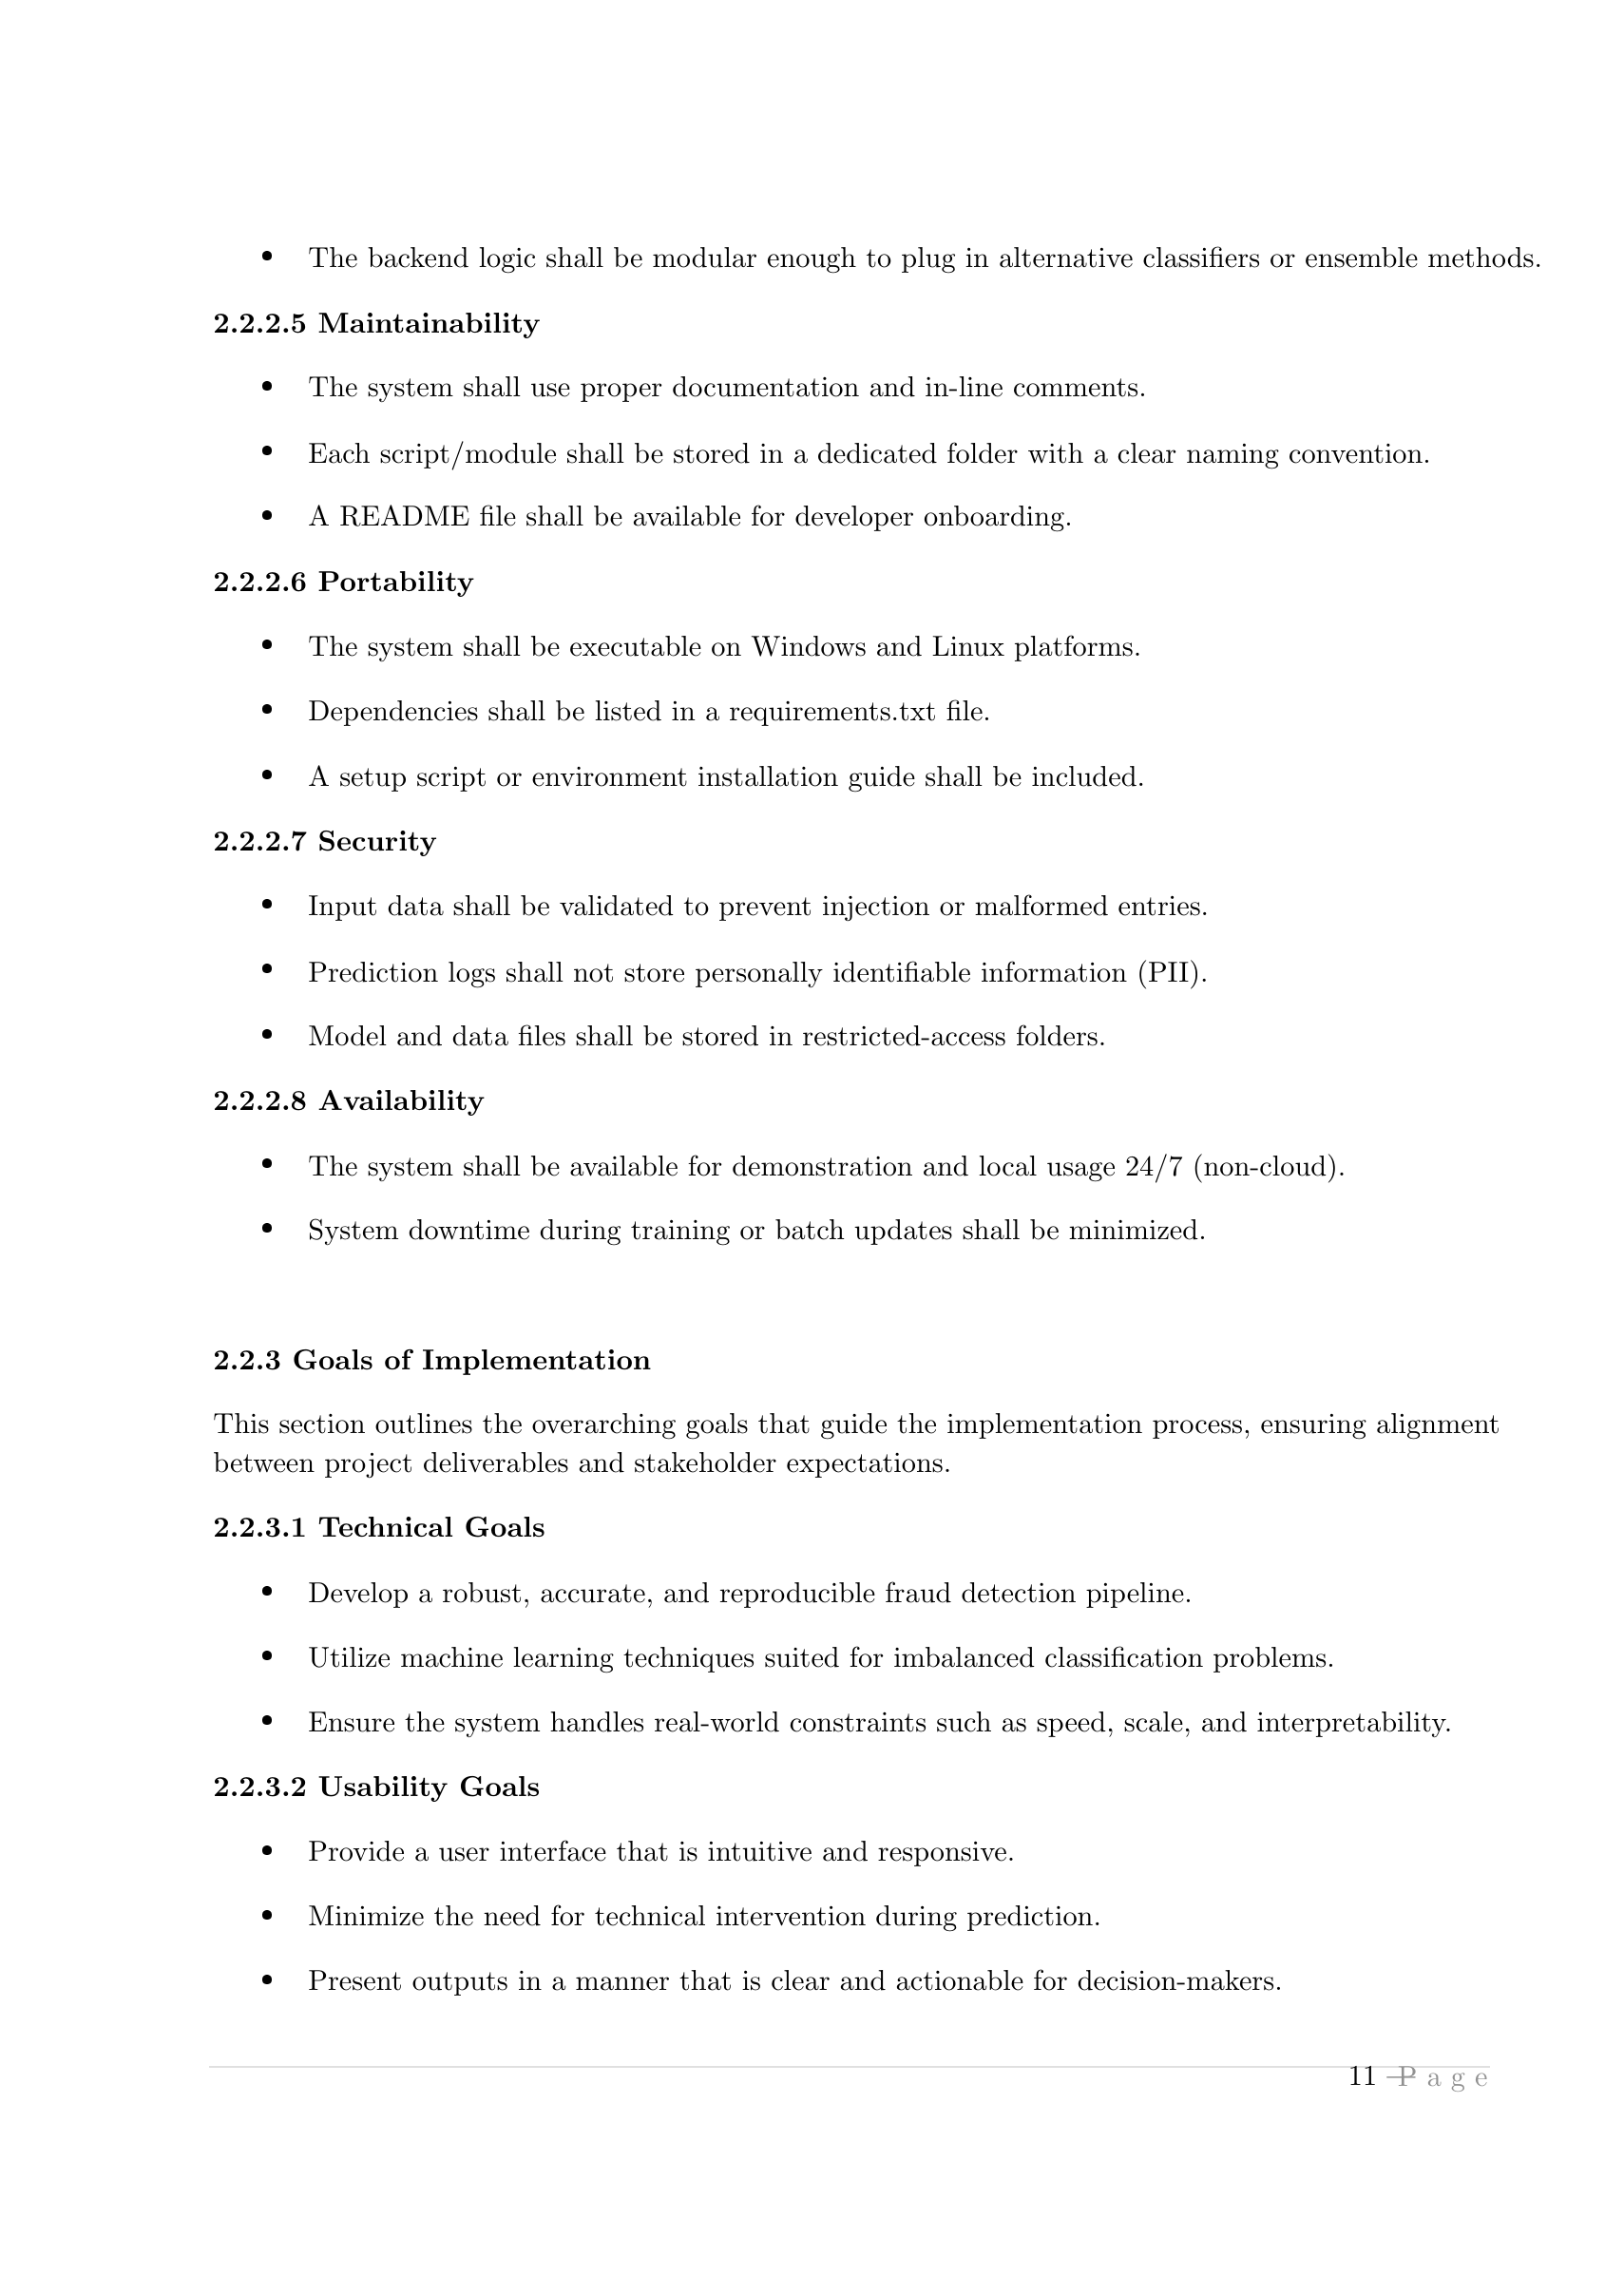
\begin{tikzpicture}[x=1bp,y=-1bp,inner sep=0pt,outer sep=0pt]
  \useasboundingbox (0,0) rectangle (595.20,841.92);
  \fill[fill=pdfcolor9] (69.38,772.78) rectangle (554.40,773.26);
  \node[anchor=north west,inner sep=0pt,outer sep=0pt] at (500.86,772.91) {{\fontsize{11.0bp}{13.2bp}\selectfont 11 | }};
  \node[anchor=north west,inner sep=0pt,outer sep=0pt] at (519.58,772.91) {{\fontsize{11.0bp}{13.2bp}\selectfont \textcolor{pdfcolor1}{P a g e}}};
  \node[anchor=north west,inner sep=0pt,outer sep=0pt] at (550.14,772.91) {{\fontsize{11.0bp}{13.2bp}\selectfont   }};
  \node[anchor=north west,inner sep=0pt,outer sep=0pt] at (88.85,85.17) {{\fontsize{10.1bp}{12.1bp}\selectfont •}};
  \node[anchor=north west,inner sep=0pt,outer sep=0pt] at (93.41,84.46) {\textsf{{\fontsize{10.1bp}{12.1bp}\selectfont  }}};
  \node[anchor=north west,inner sep=0pt,outer sep=0pt] at (106.85,83.67) {{\fontsize{11.0bp}{13.2bp}\selectfont The backend logic shall be modular enough to plug in alternative classifiers or ensemble methods. }};
  \node[anchor=north west,inner sep=0pt,outer sep=0pt] at (70.82,108.49) {{\fontsize{11.0bp}{13.2bp}\selectfont \textbf{2.2.2.5 Maintainability }}};
  \node[anchor=north west,inner sep=0pt,outer sep=0pt] at (88.85,134.40) {{\fontsize{10.1bp}{12.1bp}\selectfont •}};
  \node[anchor=north west,inner sep=0pt,outer sep=0pt] at (93.41,133.69) {\textsf{{\fontsize{10.1bp}{12.1bp}\selectfont  }}};
  \node[anchor=north west,inner sep=0pt,outer sep=0pt] at (106.85,132.90) {{\fontsize{11.0bp}{13.2bp}\selectfont The system shall use proper documentation and in-line comments. }};
  \node[anchor=north west,inner sep=0pt,outer sep=0pt] at (88.85,158.88) {{\fontsize{10.1bp}{12.1bp}\selectfont •}};
  \node[anchor=north west,inner sep=0pt,outer sep=0pt] at (93.41,158.17) {\textsf{{\fontsize{10.1bp}{12.1bp}\selectfont  }}};
  \node[anchor=north west,inner sep=0pt,outer sep=0pt] at (106.85,157.38) {{\fontsize{11.0bp}{13.2bp}\selectfont Each script/module shall be stored in a dedicated folder with a clear naming convention. }};
  \node[anchor=north west,inner sep=0pt,outer sep=0pt] at (88.85,183.36) {{\fontsize{10.1bp}{12.1bp}\selectfont •}};
  \node[anchor=north west,inner sep=0pt,outer sep=0pt] at (93.41,182.65) {\textsf{{\fontsize{10.1bp}{12.1bp}\selectfont  }}};
  \node[anchor=north west,inner sep=0pt,outer sep=0pt] at (106.85,181.86) {{\fontsize{11.0bp}{13.2bp}\selectfont A README file shall be available for developer onboarding. }};
  \node[anchor=north west,inner sep=0pt,outer sep=0pt] at (70.82,206.70) {{\fontsize{11.0bp}{13.2bp}\selectfont \textbf{2.2.2.6 Portability }}};
  \node[anchor=north west,inner sep=0pt,outer sep=0pt] at (88.85,232.58) {{\fontsize{10.1bp}{12.1bp}\selectfont •}};
  \node[anchor=north west,inner sep=0pt,outer sep=0pt] at (93.41,231.87) {\textsf{{\fontsize{10.1bp}{12.1bp}\selectfont  }}};
  \node[anchor=north west,inner sep=0pt,outer sep=0pt] at (106.85,231.08) {{\fontsize{11.0bp}{13.2bp}\selectfont The system shall be executable on Windows and Linux platforms. }};
  \node[anchor=north west,inner sep=0pt,outer sep=0pt] at (88.85,257.06) {{\fontsize{10.1bp}{12.1bp}\selectfont •}};
  \node[anchor=north west,inner sep=0pt,outer sep=0pt] at (93.41,256.35) {\textsf{{\fontsize{10.1bp}{12.1bp}\selectfont  }}};
  \node[anchor=north west,inner sep=0pt,outer sep=0pt] at (106.85,255.56) {{\fontsize{11.0bp}{13.2bp}\selectfont Dependencies shall be listed in a requirements.txt file. }};
  \node[anchor=north west,inner sep=0pt,outer sep=0pt] at (88.85,281.78) {{\fontsize{10.1bp}{12.1bp}\selectfont •}};
  \node[anchor=north west,inner sep=0pt,outer sep=0pt] at (93.41,281.07) {\textsf{{\fontsize{10.1bp}{12.1bp}\selectfont  }}};
  \node[anchor=north west,inner sep=0pt,outer sep=0pt] at (106.85,280.28) {{\fontsize{11.0bp}{13.2bp}\selectfont A setup script or environment installation guide shall be included. }};
  \node[anchor=north west,inner sep=0pt,outer sep=0pt] at (70.82,304.89) {{\fontsize{11.0bp}{13.2bp}\selectfont \textbf{2.2.2.7 Security }}};
  \node[anchor=north west,inner sep=0pt,outer sep=0pt] at (88.85,330.77) {{\fontsize{10.1bp}{12.1bp}\selectfont •}};
  \node[anchor=north west,inner sep=0pt,outer sep=0pt] at (93.41,330.06) {\textsf{{\fontsize{10.1bp}{12.1bp}\selectfont  }}};
  \node[anchor=north west,inner sep=0pt,outer sep=0pt] at (106.85,329.27) {{\fontsize{11.0bp}{13.2bp}\selectfont Input data shall be validated to prevent injection or malformed entries. }};
  \node[anchor=north west,inner sep=0pt,outer sep=0pt] at (88.85,355.25) {{\fontsize{10.1bp}{12.1bp}\selectfont •}};
  \node[anchor=north west,inner sep=0pt,outer sep=0pt] at (93.41,354.54) {\textsf{{\fontsize{10.1bp}{12.1bp}\selectfont  }}};
  \node[anchor=north west,inner sep=0pt,outer sep=0pt] at (106.85,353.75) {{\fontsize{11.0bp}{13.2bp}\selectfont Prediction logs shall not store personally identifiable information (PII). }};
  \node[anchor=north west,inner sep=0pt,outer sep=0pt] at (88.85,379.99) {{\fontsize{10.1bp}{12.1bp}\selectfont •}};
  \node[anchor=north west,inner sep=0pt,outer sep=0pt] at (93.41,379.28) {\textsf{{\fontsize{10.1bp}{12.1bp}\selectfont  }}};
  \node[anchor=north west,inner sep=0pt,outer sep=0pt] at (106.85,378.49) {{\fontsize{11.0bp}{13.2bp}\selectfont Model and data files shall be stored in restricted-access folders. }};
  \node[anchor=north west,inner sep=0pt,outer sep=0pt] at (70.82,403.07) {{\fontsize{11.0bp}{13.2bp}\selectfont \textbf{2.2.2.8 Availability }}};
  \node[anchor=north west,inner sep=0pt,outer sep=0pt] at (88.85,428.95) {{\fontsize{10.1bp}{12.1bp}\selectfont •}};
  \node[anchor=north west,inner sep=0pt,outer sep=0pt] at (93.41,428.24) {\textsf{{\fontsize{10.1bp}{12.1bp}\selectfont  }}};
  \node[anchor=north west,inner sep=0pt,outer sep=0pt] at (106.85,427.45) {{\fontsize{11.0bp}{13.2bp}\selectfont The system shall be available for demonstration and local usage 24/7 (non-cloud). }};
  \node[anchor=north west,inner sep=0pt,outer sep=0pt] at (88.85,453.67) {{\fontsize{10.1bp}{12.1bp}\selectfont •}};
  \node[anchor=north west,inner sep=0pt,outer sep=0pt] at (93.41,452.96) {\textsf{{\fontsize{10.1bp}{12.1bp}\selectfont  }}};
  \node[anchor=north west,inner sep=0pt,outer sep=0pt] at (106.85,452.17) {{\fontsize{11.0bp}{13.2bp}\selectfont System downtime during training or batch updates shall be minimized. }};
  \node[anchor=north west,inner sep=0pt,outer sep=0pt] at (70.82,501.25) {{\fontsize{11.0bp}{13.2bp}\selectfont \textbf{2.2.3 Goals of Implementation }}};
  \node[anchor=north west,inner sep=0pt,outer sep=0pt] at (70.82,525.63) {{\fontsize{11.0bp}{13.2bp}\selectfont This section outlines the overarching goals that guide the implementation process, ensuring alignment }};
  \node[anchor=north west,inner sep=0pt,outer sep=0pt] at (70.82,540.27) {{\fontsize{11.0bp}{13.2bp}\selectfont between project deliverables and stakeholder expectations. }};
  \node[anchor=north west,inner sep=0pt,outer sep=0pt] at (70.82,564.88) {{\fontsize{11.0bp}{13.2bp}\selectfont \textbf{2.2.3.1 Technical Goals }}};
  \node[anchor=north west,inner sep=0pt,outer sep=0pt] at (88.85,591.00) {{\fontsize{10.1bp}{12.1bp}\selectfont •}};
  \node[anchor=north west,inner sep=0pt,outer sep=0pt] at (93.41,590.29) {\textsf{{\fontsize{10.1bp}{12.1bp}\selectfont  }}};
  \node[anchor=north west,inner sep=0pt,outer sep=0pt] at (106.85,589.50) {{\fontsize{11.0bp}{13.2bp}\selectfont Develop a robust, accurate, and reproducible fraud detection pipeline. }};
  \node[anchor=north west,inner sep=0pt,outer sep=0pt] at (88.85,615.48) {{\fontsize{10.1bp}{12.1bp}\selectfont •}};
  \node[anchor=north west,inner sep=0pt,outer sep=0pt] at (93.41,614.77) {\textsf{{\fontsize{10.1bp}{12.1bp}\selectfont  }}};
  \node[anchor=north west,inner sep=0pt,outer sep=0pt] at (106.85,613.98) {{\fontsize{11.0bp}{13.2bp}\selectfont Utilize machine learning techniques suited for imbalanced classification problems. }};
  \node[anchor=north west,inner sep=0pt,outer sep=0pt] at (88.85,639.98) {{\fontsize{10.1bp}{12.1bp}\selectfont •}};
  \node[anchor=north west,inner sep=0pt,outer sep=0pt] at (93.41,639.27) {\textsf{{\fontsize{10.1bp}{12.1bp}\selectfont  }}};
  \node[anchor=north west,inner sep=0pt,outer sep=0pt] at (106.85,638.48) {{\fontsize{11.0bp}{13.2bp}\selectfont Ensure the system handles real-world constraints such as speed, scale, and interpretability. }};
  \node[anchor=north west,inner sep=0pt,outer sep=0pt] at (70.82,663.06) {{\fontsize{11.0bp}{13.2bp}\selectfont \textbf{2.2.3.2 Usability Goals }}};
  \node[anchor=north west,inner sep=0pt,outer sep=0pt] at (88.85,689.18) {{\fontsize{10.1bp}{12.1bp}\selectfont •}};
  \node[anchor=north west,inner sep=0pt,outer sep=0pt] at (93.41,688.47) {\textsf{{\fontsize{10.1bp}{12.1bp}\selectfont  }}};
  \node[anchor=north west,inner sep=0pt,outer sep=0pt] at (106.85,687.68) {{\fontsize{11.0bp}{13.2bp}\selectfont Provide a user interface that is intuitive and responsive. }};
  \node[anchor=north west,inner sep=0pt,outer sep=0pt] at (88.85,713.66) {{\fontsize{10.1bp}{12.1bp}\selectfont •}};
  \node[anchor=north west,inner sep=0pt,outer sep=0pt] at (93.41,712.95) {\textsf{{\fontsize{10.1bp}{12.1bp}\selectfont  }}};
  \node[anchor=north west,inner sep=0pt,outer sep=0pt] at (106.85,712.16) {{\fontsize{11.0bp}{13.2bp}\selectfont Minimize the need for technical intervention during prediction. }};
  \node[anchor=north west,inner sep=0pt,outer sep=0pt] at (88.85,738.16) {{\fontsize{10.1bp}{12.1bp}\selectfont •}};
  \node[anchor=north west,inner sep=0pt,outer sep=0pt] at (93.41,737.46) {\textsf{{\fontsize{10.1bp}{12.1bp}\selectfont  }}};
  \node[anchor=north west,inner sep=0pt,outer sep=0pt] at (106.85,736.67) {{\fontsize{11.0bp}{13.2bp}\selectfont Present outputs in a manner that is clear and actionable for decision-makers. }};
\end{tikzpicture}
\newpage
\noindent
\begin{tikzpicture}[x=1bp,y=-1bp,inner sep=0pt,outer sep=0pt]
  \useasboundingbox (0,0) rectangle (595.20,841.92);
  \fill[fill=pdfcolor9] (69.38,772.78) rectangle (554.40,773.26);
  \fill[fill=black] (142.87,531.50) rectangle (470.35,532.94);
  \fill[fill=black] (70.82,565.61) rectangle (194.47,567.05);
  \node[anchor=north west,inner sep=0pt] at (70.90,585.18) {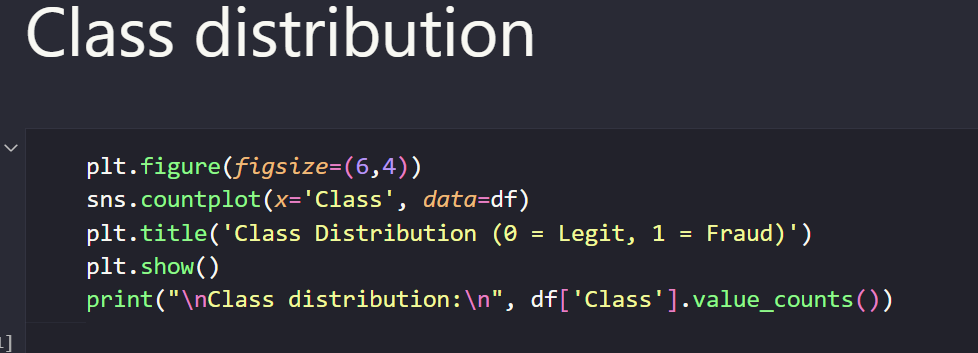
\includegraphics[width=468.00bp,height=168.90bp]{images/image_p20_3.png}};
  \node[anchor=north west,inner sep=0pt,outer sep=0pt] at (500.86,772.91) {{\fontsize{11.0bp}{13.2bp}\selectfont 12 | }};
  \node[anchor=north west,inner sep=0pt,outer sep=0pt] at (519.58,772.91) {{\fontsize{11.0bp}{13.2bp}\selectfont \textcolor{pdfcolor1}{P a g e}}};
  \node[anchor=north west,inner sep=0pt,outer sep=0pt] at (550.14,772.91) {{\fontsize{11.0bp}{13.2bp}\selectfont   }};
  \node[anchor=north west,inner sep=0pt,outer sep=0pt] at (70.82,108.49) {{\fontsize{11.0bp}{13.2bp}\selectfont \textbf{2.2.3.3 Deployment Goals }}};
  \node[anchor=north west,inner sep=0pt,outer sep=0pt] at (88.85,134.40) {{\fontsize{10.1bp}{12.1bp}\selectfont •}};
  \node[anchor=north west,inner sep=0pt,outer sep=0pt] at (93.41,133.69) {\textsf{{\fontsize{10.1bp}{12.1bp}\selectfont  }}};
  \node[anchor=north west,inner sep=0pt,outer sep=0pt] at (106.85,132.90) {{\fontsize{11.0bp}{13.2bp}\selectfont Enable seamless model deployment through Streamlit. }};
  \node[anchor=north west,inner sep=0pt,outer sep=0pt] at (88.85,158.88) {{\fontsize{10.1bp}{12.1bp}\selectfont •}};
  \node[anchor=north west,inner sep=0pt,outer sep=0pt] at (93.41,158.17) {\textsf{{\fontsize{10.1bp}{12.1bp}\selectfont  }}};
  \node[anchor=north west,inner sep=0pt,outer sep=0pt] at (106.85,157.38) {{\fontsize{11.0bp}{13.2bp}\selectfont Support easy migration to cloud platforms for future scalability. }};
  \node[anchor=north west,inner sep=0pt,outer sep=0pt] at (88.85,183.36) {{\fontsize{10.1bp}{12.1bp}\selectfont •}};
  \node[anchor=north west,inner sep=0pt,outer sep=0pt] at (93.41,182.65) {\textsf{{\fontsize{10.1bp}{12.1bp}\selectfont  }}};
  \node[anchor=north west,inner sep=0pt,outer sep=0pt] at (106.85,181.86) {{\fontsize{11.0bp}{13.2bp}\selectfont Allow integration with external systems via API in extended versions. }};
  \node[anchor=north west,inner sep=0pt,outer sep=0pt] at (70.82,206.70) {{\fontsize{11.0bp}{13.2bp}\selectfont \textbf{2.2.3.4 Educational Goals }}};
  \node[anchor=north west,inner sep=0pt,outer sep=0pt] at (88.85,232.58) {{\fontsize{10.1bp}{12.1bp}\selectfont •}};
  \node[anchor=north west,inner sep=0pt,outer sep=0pt] at (93.41,231.87) {\textsf{{\fontsize{10.1bp}{12.1bp}\selectfont  }}};
  \node[anchor=north west,inner sep=0pt,outer sep=0pt] at (106.85,231.08) {{\fontsize{11.0bp}{13.2bp}\selectfont Create a full-stack reference project for students and researchers. }};
  \node[anchor=north west,inner sep=0pt,outer sep=0pt] at (88.85,257.06) {{\fontsize{10.1bp}{12.1bp}\selectfont •}};
  \node[anchor=north west,inner sep=0pt,outer sep=0pt] at (93.41,256.35) {\textsf{{\fontsize{10.1bp}{12.1bp}\selectfont  }}};
  \node[anchor=north west,inner sep=0pt,outer sep=0pt] at (106.85,255.56) {{\fontsize{11.0bp}{13.2bp}\selectfont Demonstrate best practices in machine learning pipeline construction. }};
  \node[anchor=north west,inner sep=0pt,outer sep=0pt] at (88.85,281.78) {{\fontsize{10.1bp}{12.1bp}\selectfont •}};
  \node[anchor=north west,inner sep=0pt,outer sep=0pt] at (93.41,281.07) {\textsf{{\fontsize{10.1bp}{12.1bp}\selectfont  }}};
  \node[anchor=north west,inner sep=0pt,outer sep=0pt] at (106.85,280.28) {{\fontsize{11.0bp}{13.2bp}\selectfont Enable experimentation and learning through clear modularization. }};
  \node[anchor=north west,inner sep=0pt,outer sep=0pt] at (70.82,304.89) {{\fontsize{11.0bp}{13.2bp}\selectfont \textbf{2.2.3.5 Innovation Goals }}};
  \node[anchor=north west,inner sep=0pt,outer sep=0pt] at (88.85,330.77) {{\fontsize{10.1bp}{12.1bp}\selectfont •}};
  \node[anchor=north west,inner sep=0pt,outer sep=0pt] at (93.41,330.06) {\textsf{{\fontsize{10.1bp}{12.1bp}\selectfont  }}};
  \node[anchor=north west,inner sep=0pt,outer sep=0pt] at (106.85,329.27) {{\fontsize{11.0bp}{13.2bp}\selectfont Promote the use of machine learning for financial fraud risk management. }};
  \node[anchor=north west,inner sep=0pt,outer sep=0pt] at (88.85,355.25) {{\fontsize{10.1bp}{12.1bp}\selectfont •}};
  \node[anchor=north west,inner sep=0pt,outer sep=0pt] at (93.41,354.54) {\textsf{{\fontsize{10.1bp}{12.1bp}\selectfont  }}};
  \node[anchor=north west,inner sep=0pt,outer sep=0pt] at (106.85,353.75) {{\fontsize{11.0bp}{13.2bp}\selectfont Showcase the importance of real-time prediction and explainable AI in fintech. }};
  \node[anchor=north west,inner sep=0pt,outer sep=0pt] at (88.85,379.99) {{\fontsize{10.1bp}{12.1bp}\selectfont •}};
  \node[anchor=north west,inner sep=0pt,outer sep=0pt] at (93.41,379.28) {\textsf{{\fontsize{10.1bp}{12.1bp}\selectfont  }}};
  \node[anchor=north west,inner sep=0pt,outer sep=0pt] at (106.85,378.49) {{\fontsize{11.0bp}{13.2bp}\selectfont Inspire future enhancements including dynamic learning and unsupervised detection. }};
  \node[anchor=north west,inner sep=0pt,outer sep=0pt] at (70.82,402.97) {{\fontsize{11.0bp}{13.2bp}\selectfont By fulfilling these goals, the project ensures that it provides immediate practical value while also offering a }};
  \node[anchor=north west,inner sep=0pt,outer sep=0pt] at (70.82,417.61) {{\fontsize{11.0bp}{13.2bp}\selectfont scalable foundation for future innovation and academic study. }};
  \node[anchor=north west,inner sep=0pt,outer sep=0pt] at (142.87,515.53) {{\fontsize{13.9bp}{16.7bp}\selectfont \textbf{2.3 DATA ANALYSIS AND DATA VISUALISATION }}};
  \node[anchor=north west,inner sep=0pt,outer sep=0pt] at (70.82,549.64) {{\fontsize{13.9bp}{16.7bp}\selectfont \textbf{1 Class Distribution: }}};
\end{tikzpicture}
\newpage
\noindent
\begin{tikzpicture}[x=1bp,y=-1bp,inner sep=0pt,outer sep=0pt]
  \useasboundingbox (0,0) rectangle (595.20,841.92);
  \fill[fill=pdfcolor9] (69.38,772.78) rectangle (554.40,773.26);
  \node[anchor=north west,inner sep=0pt] at (70.90,85.05) {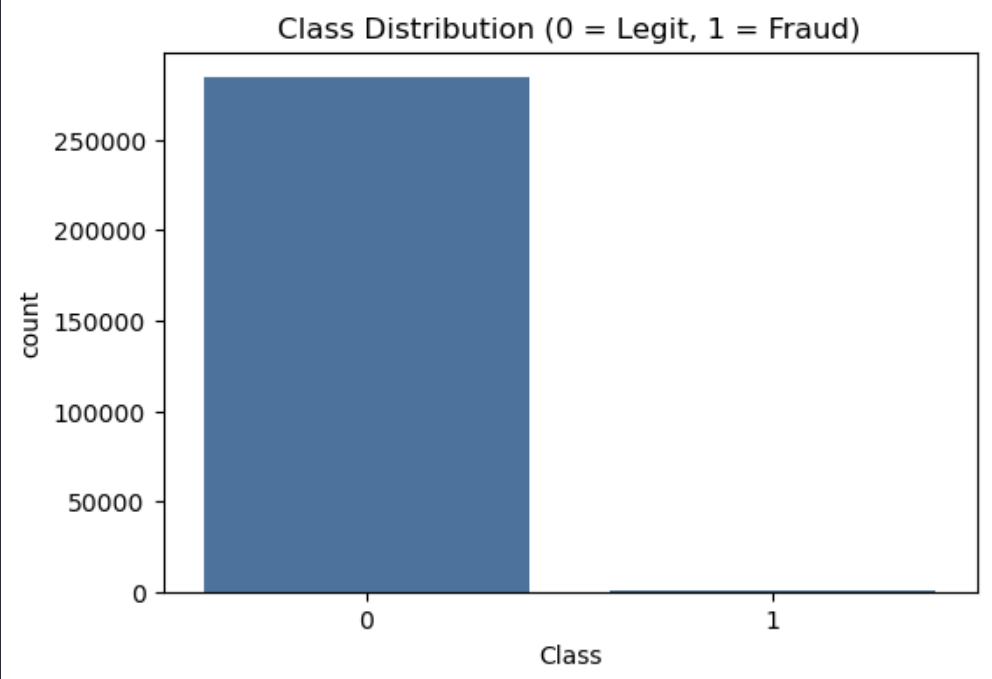
\includegraphics[width=468.00bp,height=320.30bp]{images/image_p21_4.png}};
  \node[anchor=north west,inner sep=0pt] at (70.90,417.95) {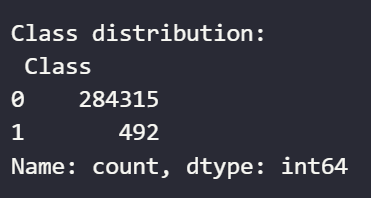
\includegraphics[width=482.10bp,height=257.29bp]{images/image_p21_5.png}};
  \node[anchor=north west,inner sep=0pt,outer sep=0pt] at (500.86,772.91) {{\fontsize{11.0bp}{13.2bp}\selectfont 13 | }};
  \node[anchor=north west,inner sep=0pt,outer sep=0pt] at (519.58,772.91) {{\fontsize{11.0bp}{13.2bp}\selectfont \textcolor{pdfcolor1}{P a g e}}};
  \node[anchor=north west,inner sep=0pt,outer sep=0pt] at (550.14,772.91) {{\fontsize{11.0bp}{13.2bp}\selectfont   }};
\end{tikzpicture}
\newpage
\noindent
\begin{tikzpicture}[x=1bp,y=-1bp,inner sep=0pt,outer sep=0pt]
  \useasboundingbox (0,0) rectangle (595.20,841.92);
  \fill[fill=pdfcolor9] (69.38,772.78) rectangle (554.40,773.26);
  \fill[fill=black] (70.82,99.38) rectangle (261.48,100.82);
  \fill[fill=black] (70.82,561.05) rectangle (200.01,562.49);
  \node[anchor=north west,inner sep=0pt] at (70.90,119.20) {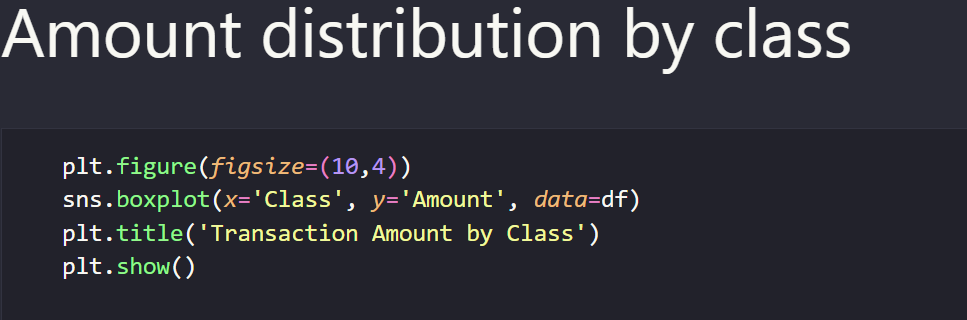
\includegraphics[width=468.00bp,height=154.85bp]{images/image_p22_6.png}};
  \node[anchor=north west,inner sep=0pt] at (70.90,310.49) {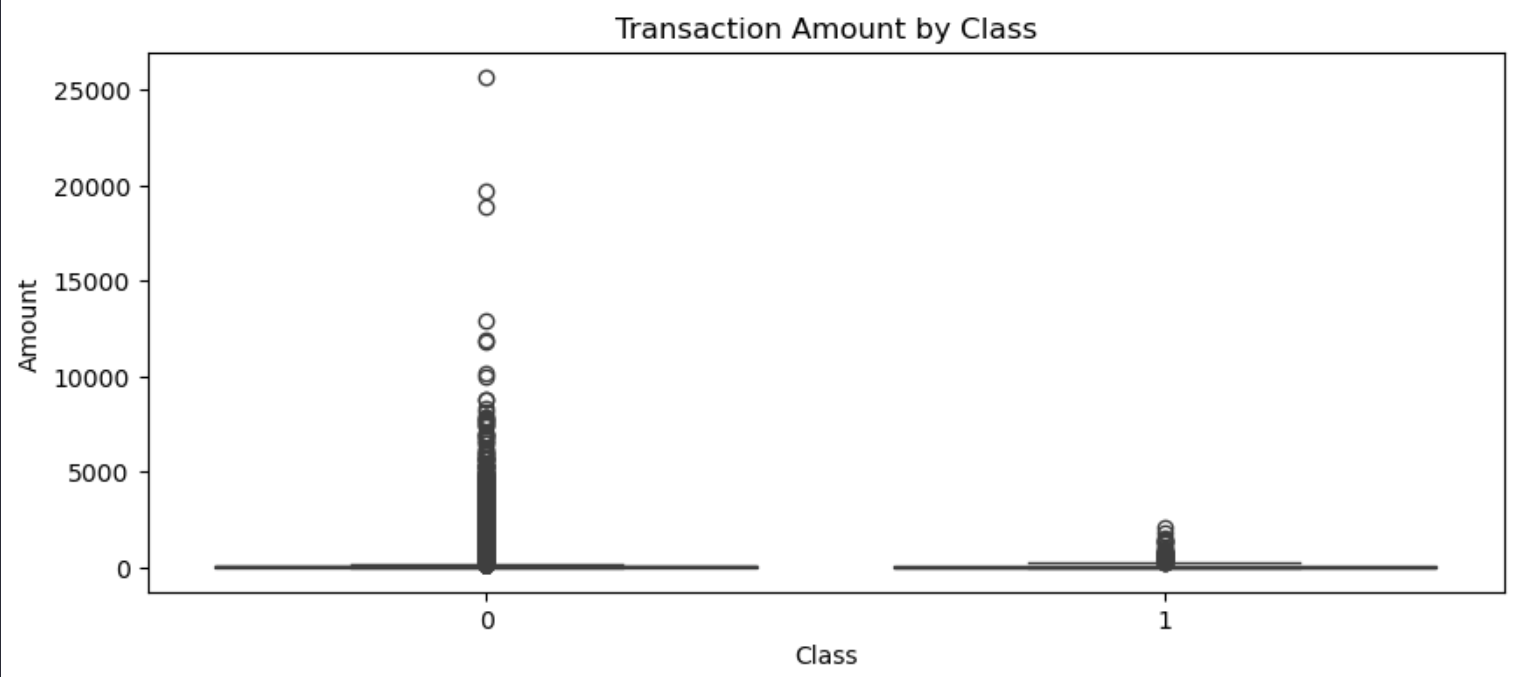
\includegraphics[width=442.15bp,height=199.18bp]{images/image_p22_7.png}};
  \node[anchor=north west,inner sep=0pt] at (70.90,580.58) {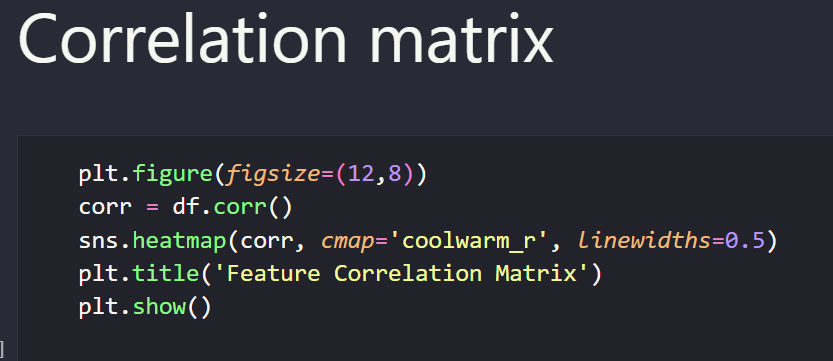
\includegraphics[width=436.15bp,height=189.00bp]{images/image_p22_8.png}};
  \node[anchor=north west,inner sep=0pt,outer sep=0pt] at (500.86,772.91) {{\fontsize{11.0bp}{13.2bp}\selectfont 14 | }};
  \node[anchor=north west,inner sep=0pt,outer sep=0pt] at (519.58,772.91) {{\fontsize{11.0bp}{13.2bp}\selectfont \textcolor{pdfcolor1}{P a g e}}};
  \node[anchor=north west,inner sep=0pt,outer sep=0pt] at (550.14,772.91) {{\fontsize{11.0bp}{13.2bp}\selectfont   }};
  \node[anchor=north west,inner sep=0pt,outer sep=0pt] at (70.82,83.41) {{\fontsize{13.9bp}{16.7bp}\selectfont \textbf{2 Amount Distribution by class: }}};
  \node[anchor=north west,inner sep=0pt,outer sep=0pt] at (70.82,545.08) {{\fontsize{13.9bp}{16.7bp}\selectfont \textbf{3 Correlation matrix: }}};
\end{tikzpicture}
\newpage
\noindent
\begin{tikzpicture}[x=1bp,y=-1bp,inner sep=0pt,outer sep=0pt]
  \useasboundingbox (0,0) rectangle (595.20,841.92);
  \fill[fill=pdfcolor9] (69.38,772.78) rectangle (554.40,773.26);
  \fill[fill=black] (70.82,486.14) rectangle (212.49,487.58);
  \node[anchor=north west,inner sep=0pt] at (70.90,85.05) {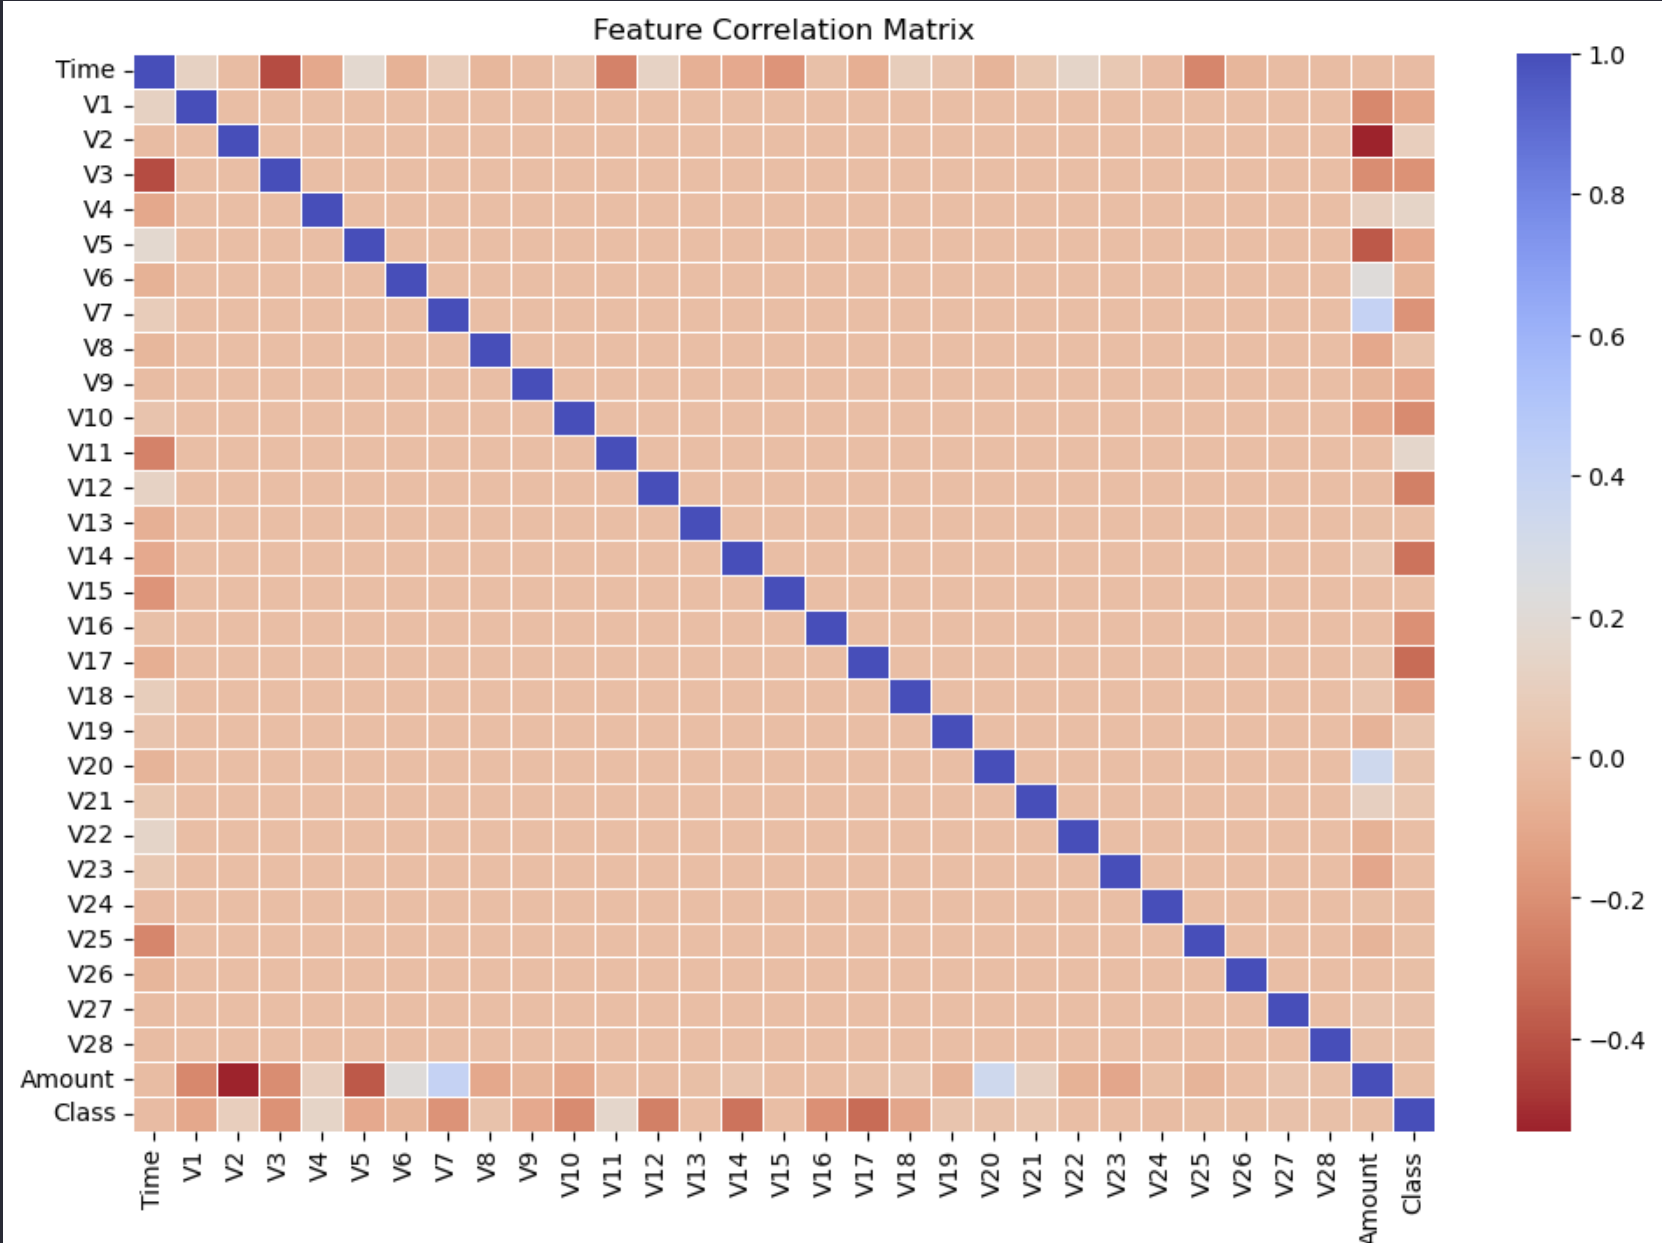
\includegraphics[width=468.00bp,height=350.00bp]{images/image_p23_9.png}};
  \node[anchor=north west,inner sep=0pt] at (70.90,530.19) {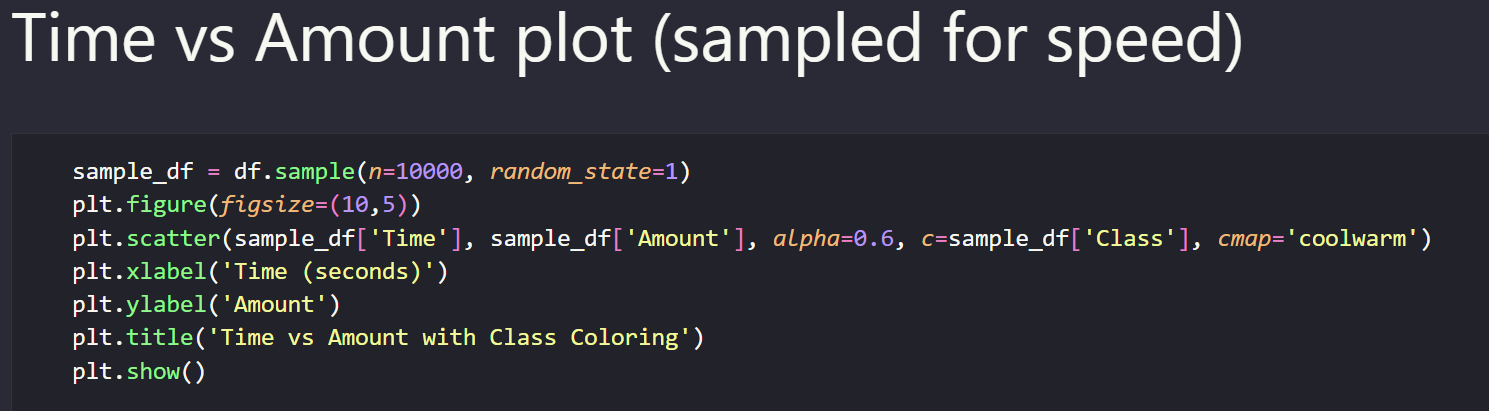
\includegraphics[width=468.00bp,height=129.15bp]{images/image_p23_10.png}};
  \node[anchor=north west,inner sep=0pt,outer sep=0pt] at (500.86,772.91) {{\fontsize{11.0bp}{13.2bp}\selectfont 15 | }};
  \node[anchor=north west,inner sep=0pt,outer sep=0pt] at (519.58,772.91) {{\fontsize{11.0bp}{13.2bp}\selectfont \textcolor{pdfcolor1}{P a g e}}};
  \node[anchor=north west,inner sep=0pt,outer sep=0pt] at (550.14,772.91) {{\fontsize{11.0bp}{13.2bp}\selectfont   }};
  \node[anchor=north west,inner sep=0pt,outer sep=0pt] at (70.82,470.17) {{\fontsize{13.9bp}{16.7bp}\selectfont \textbf{4 Time vs Amount plot: }}};
\end{tikzpicture}
\newpage
\noindent
\begin{tikzpicture}[x=1bp,y=-1bp,inner sep=0pt,outer sep=0pt]
  \useasboundingbox (0,0) rectangle (595.20,841.92);
  \fill[fill=pdfcolor9] (69.38,772.78) rectangle (554.40,773.26);
  \fill[fill=black] (70.82,391.08) rectangle (206.49,392.52);
  \node[anchor=north west,inner sep=0pt] at (70.90,85.05) {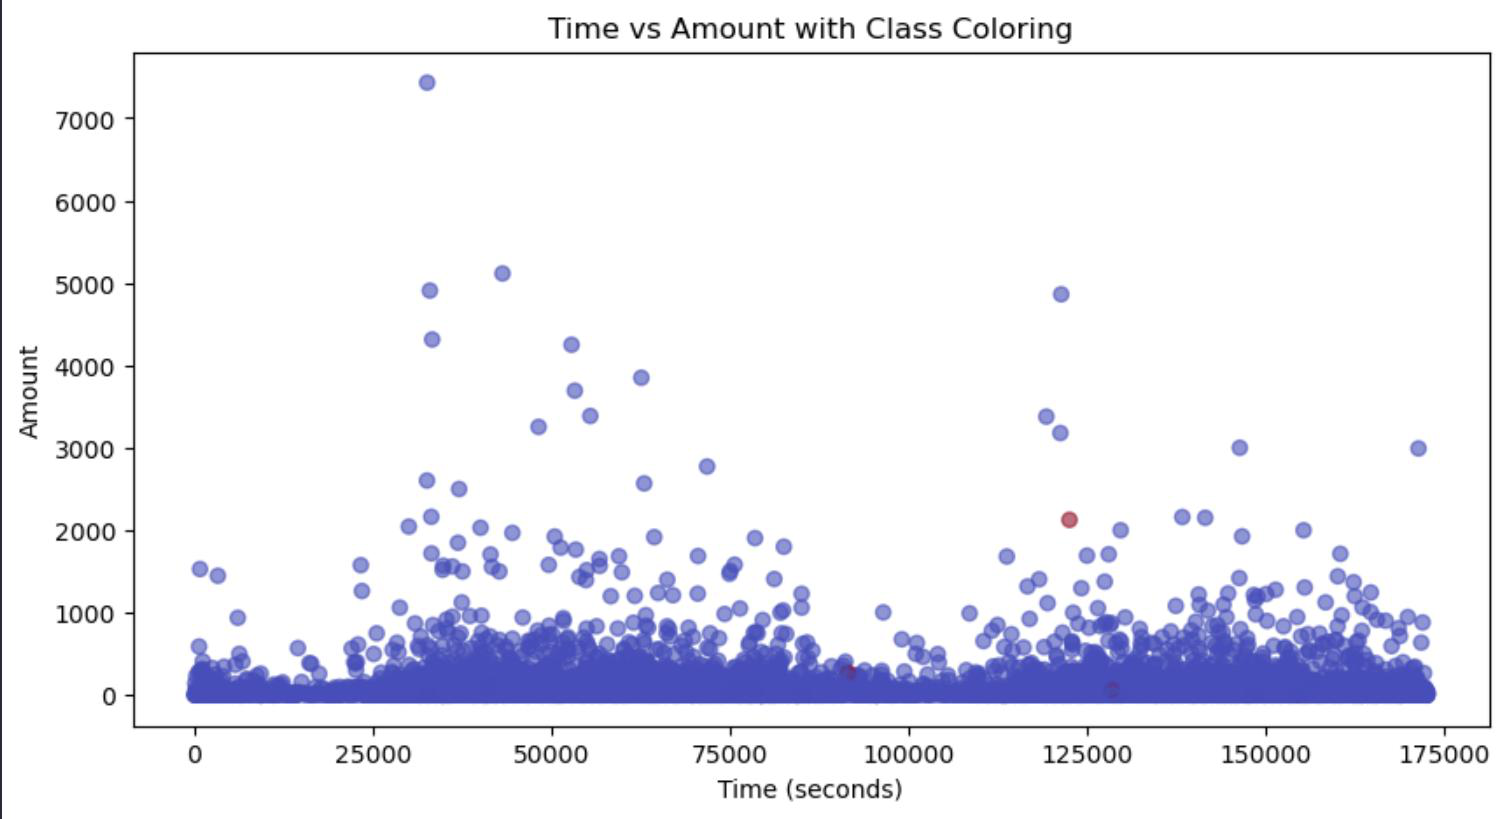
\includegraphics[width=468.00bp,height=254.35bp]{images/image_p24_11.png}};
  \node[anchor=north west,inner sep=0pt] at (70.90,433.52) {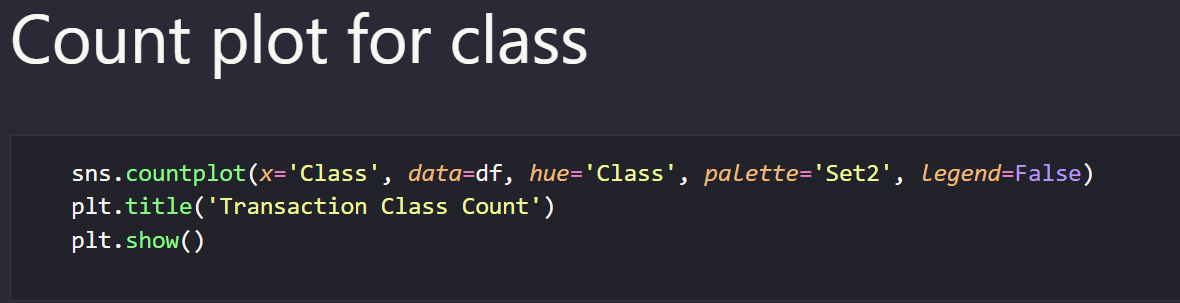
\includegraphics[width=468.00bp,height=120.15bp]{images/image_p24_12.png}};
  \node[anchor=north west,inner sep=0pt,outer sep=0pt] at (500.86,772.91) {{\fontsize{11.0bp}{13.2bp}\selectfont 16 | }};
  \node[anchor=north west,inner sep=0pt,outer sep=0pt] at (519.58,772.91) {{\fontsize{11.0bp}{13.2bp}\selectfont \textcolor{pdfcolor1}{P a g e}}};
  \node[anchor=north west,inner sep=0pt,outer sep=0pt] at (550.14,772.91) {{\fontsize{11.0bp}{13.2bp}\selectfont   }};
  \node[anchor=north west,inner sep=0pt,outer sep=0pt] at (70.82,375.11) {{\fontsize{13.9bp}{16.7bp}\selectfont \textbf{5. Count plot for class: }}};
\end{tikzpicture}
\newpage
\noindent
\begin{tikzpicture}[x=1bp,y=-1bp,inner sep=0pt,outer sep=0pt]
  \useasboundingbox (0,0) rectangle (595.20,841.92);
  \fill[fill=pdfcolor9] (69.38,772.78) rectangle (554.40,773.26);
  \fill[fill=black] (70.82,405.48) rectangle (285.48,406.92);
  \node[anchor=north west,inner sep=0pt] at (70.90,85.05) {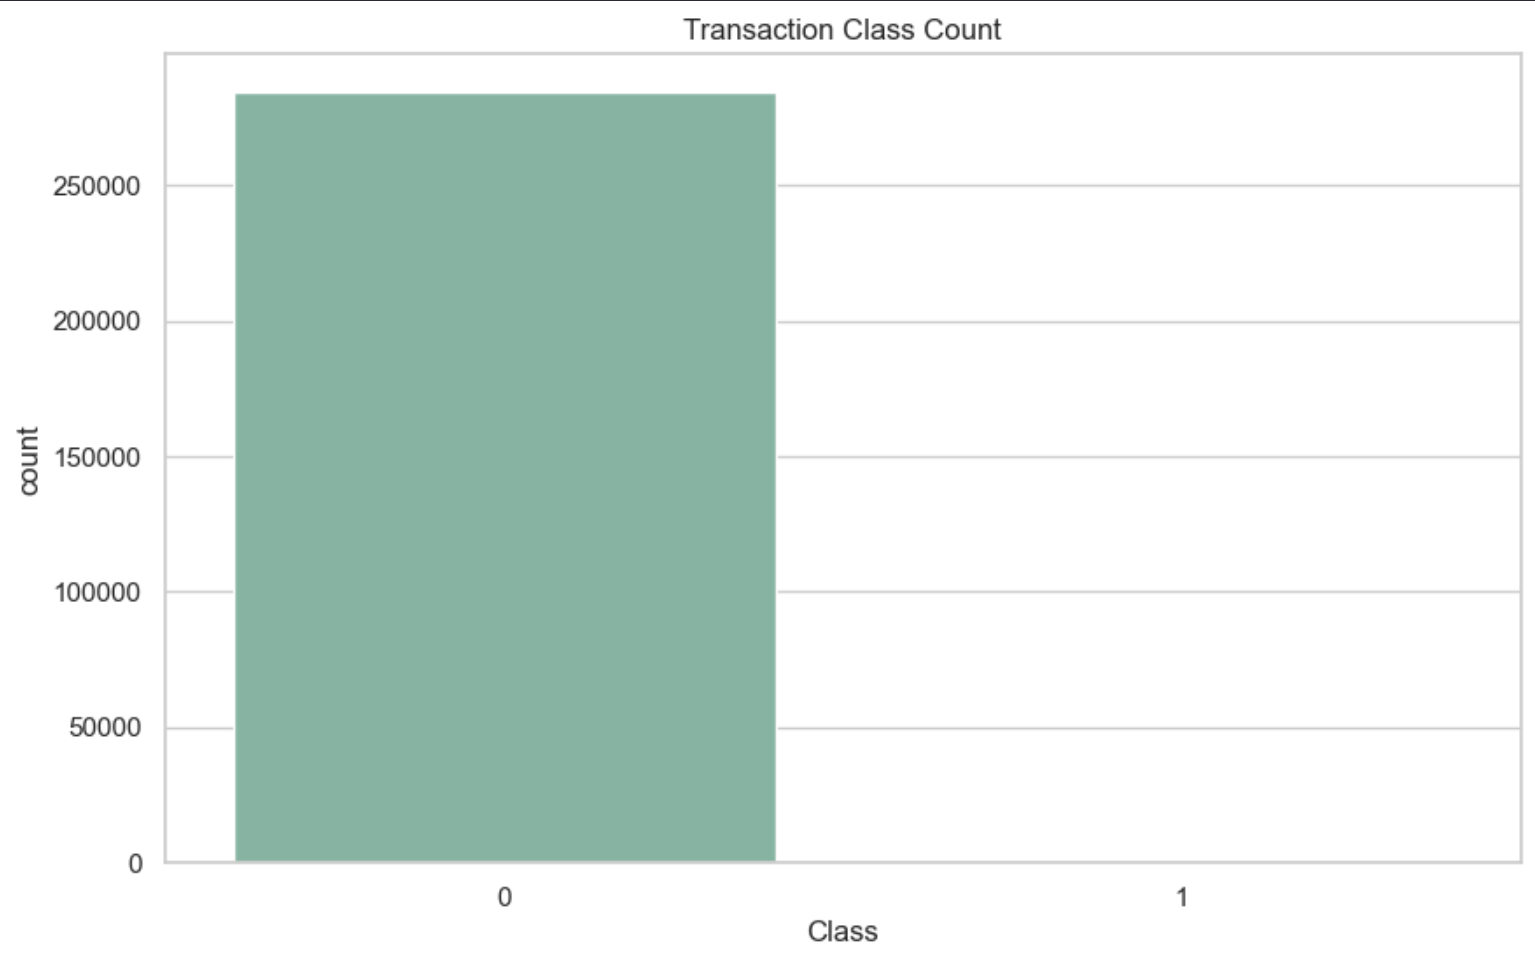
\includegraphics[width=468.00bp,height=293.30bp]{images/image_p25_13.png}};
  \node[anchor=north west,inner sep=0pt] at (70.90,419.46) {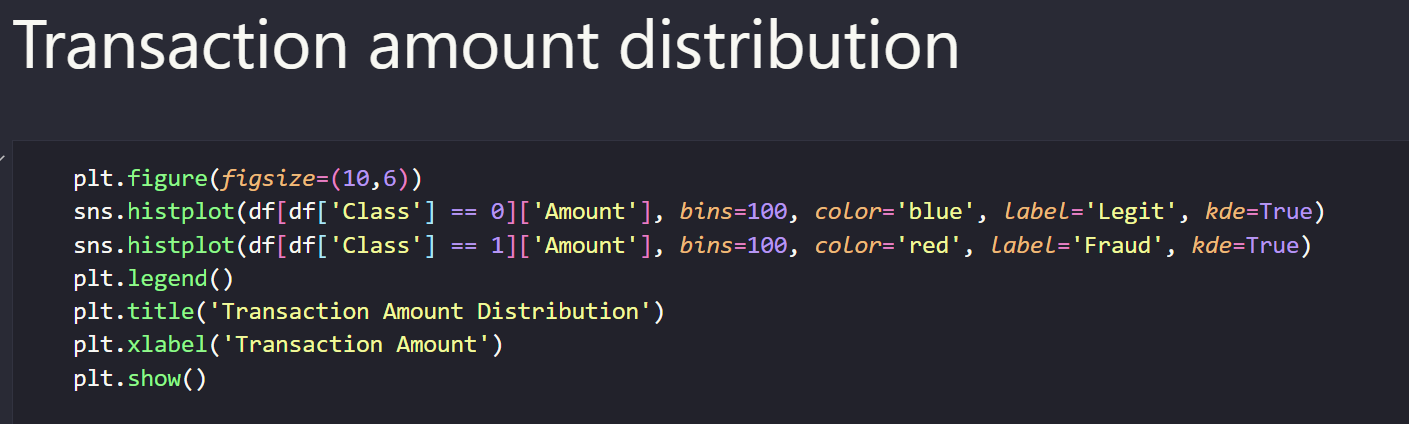
\includegraphics[width=468.00bp,height=140.80bp]{images/image_p25_14.png}};
  \node[anchor=north west,inner sep=0pt,outer sep=0pt] at (500.86,772.91) {{\fontsize{11.0bp}{13.2bp}\selectfont 17 | }};
  \node[anchor=north west,inner sep=0pt,outer sep=0pt] at (519.58,772.91) {{\fontsize{11.0bp}{13.2bp}\selectfont \textcolor{pdfcolor1}{P a g e}}};
  \node[anchor=north west,inner sep=0pt,outer sep=0pt] at (550.14,772.91) {{\fontsize{11.0bp}{13.2bp}\selectfont   }};
  \node[anchor=north west,inner sep=0pt,outer sep=0pt] at (70.82,389.51) {{\fontsize{13.9bp}{16.7bp}\selectfont \textbf{6. Transaction amount distribution: }}};
\end{tikzpicture}
\newpage
\noindent
\begin{tikzpicture}[x=1bp,y=-1bp,inner sep=0pt,outer sep=0pt]
  \useasboundingbox (0,0) rectangle (595.20,841.92);
  \fill[fill=pdfcolor9] (69.38,772.78) rectangle (554.40,773.26);
  \fill[fill=black] (70.82,453.24) rectangle (253.80,454.68);
  \node[anchor=north west,inner sep=0pt] at (70.90,85.05) {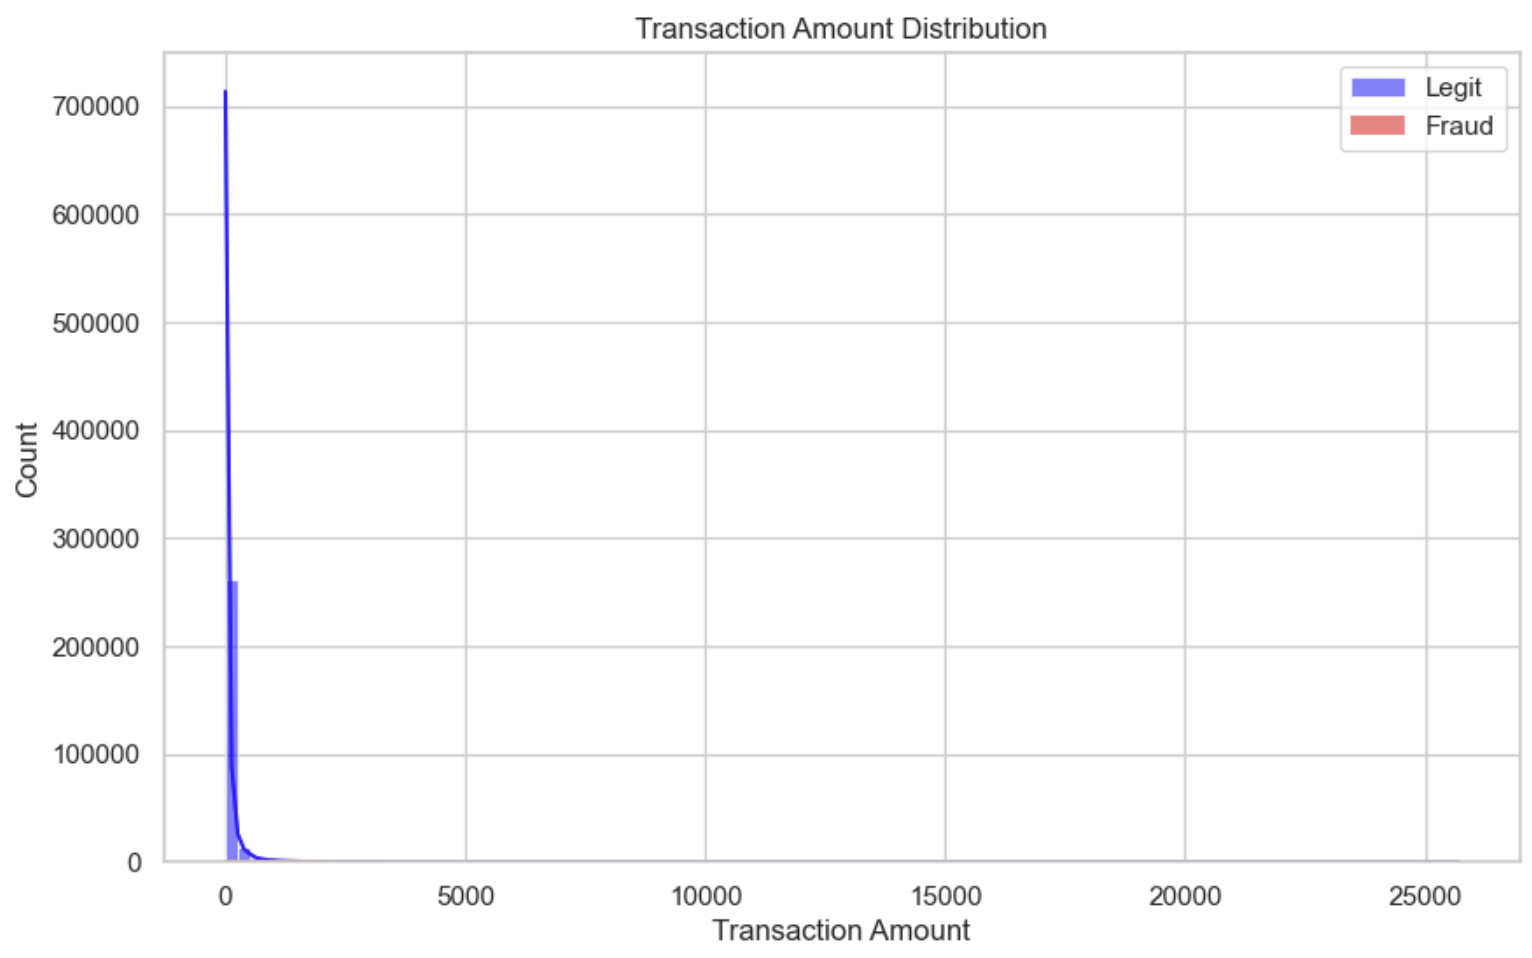
\includegraphics[width=468.00bp,height=292.65bp]{images/image_p26_15.png}};
  \node[anchor=north west,inner sep=0pt] at (70.90,495.72) {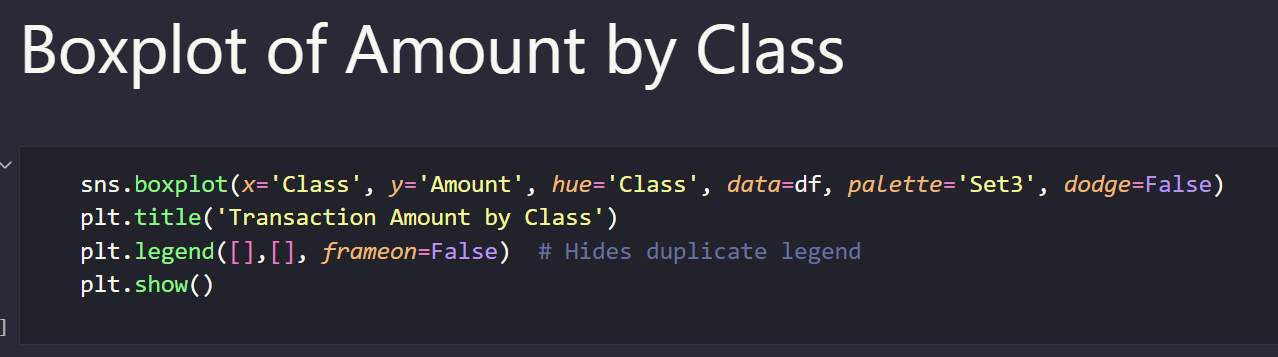
\includegraphics[width=468.00bp,height=130.70bp]{images/image_p26_16.png}};
  \node[anchor=north west,inner sep=0pt,outer sep=0pt] at (500.86,772.91) {{\fontsize{11.0bp}{13.2bp}\selectfont 18 | }};
  \node[anchor=north west,inner sep=0pt,outer sep=0pt] at (519.58,772.91) {{\fontsize{11.0bp}{13.2bp}\selectfont \textcolor{pdfcolor1}{P a g e}}};
  \node[anchor=north west,inner sep=0pt,outer sep=0pt] at (550.14,772.91) {{\fontsize{11.0bp}{13.2bp}\selectfont   }};
  \node[anchor=north west,inner sep=0pt,outer sep=0pt] at (70.82,437.27) {{\fontsize{13.9bp}{16.7bp}\selectfont \textbf{7. Boxplot of Amount by class: }}};
\end{tikzpicture}
\newpage
\noindent
\begin{tikzpicture}[x=1bp,y=-1bp,inner sep=0pt,outer sep=0pt]
  \useasboundingbox (0,0) rectangle (595.20,841.92);
  \fill[fill=pdfcolor9] (69.38,772.78) rectangle (554.40,773.26);
  \fill[fill=black] (74.42,423.96) rectangle (290.28,425.40);
  \node[anchor=north west,inner sep=0pt] at (70.90,85.05) {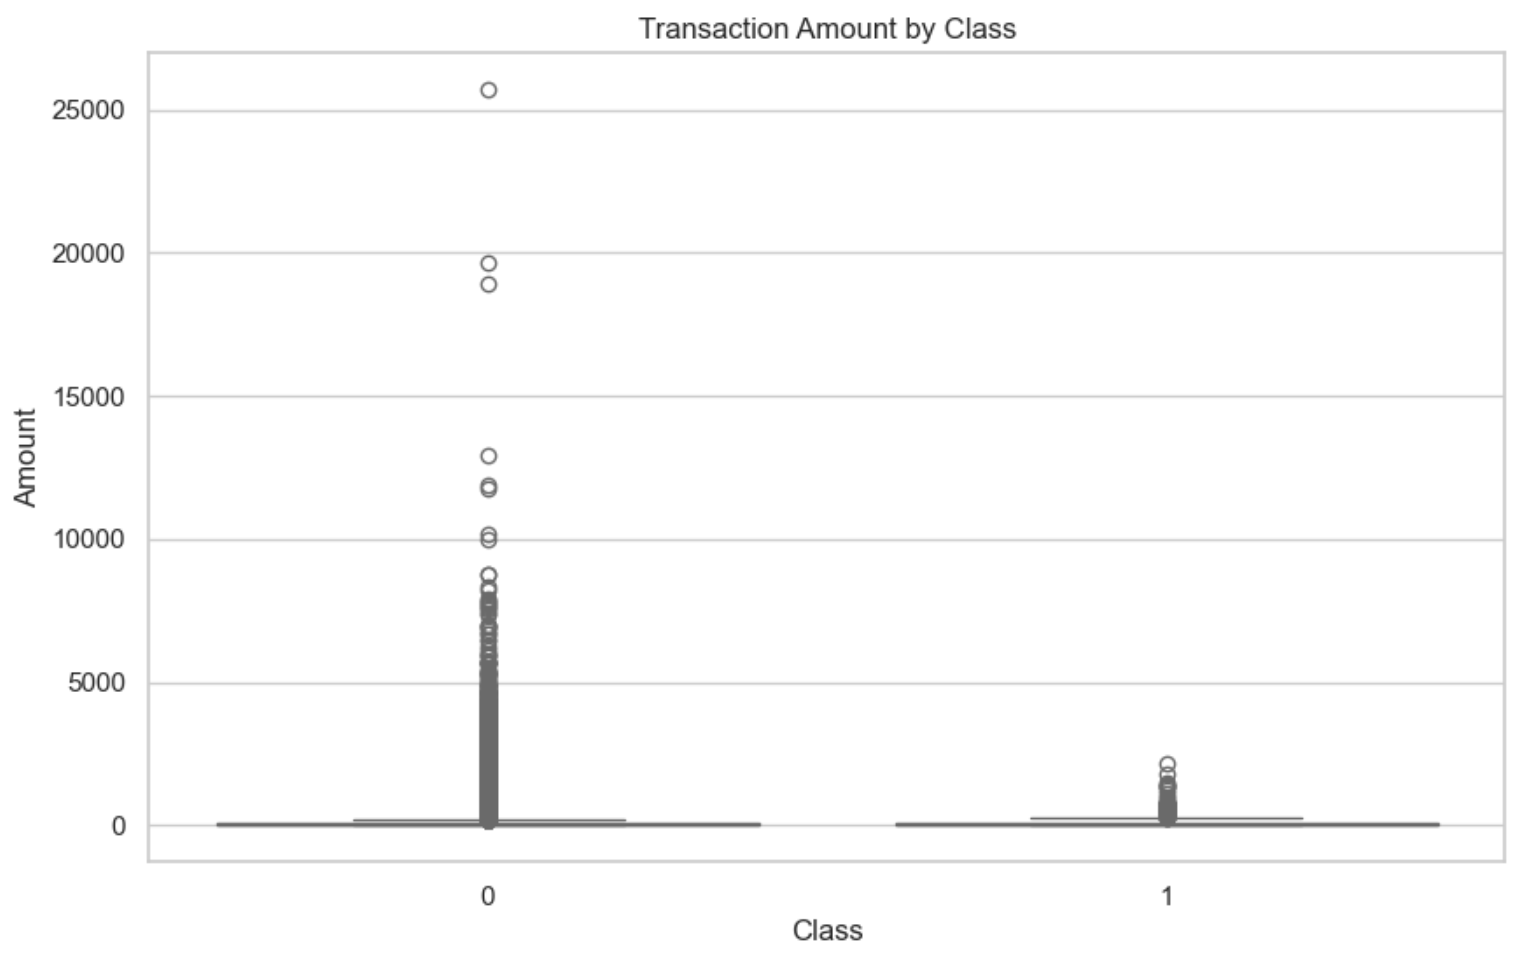
\includegraphics[width=456.80bp,height=287.55bp]{images/image_p27_17.png}};
  \node[anchor=north west,inner sep=0pt] at (70.90,466.52) {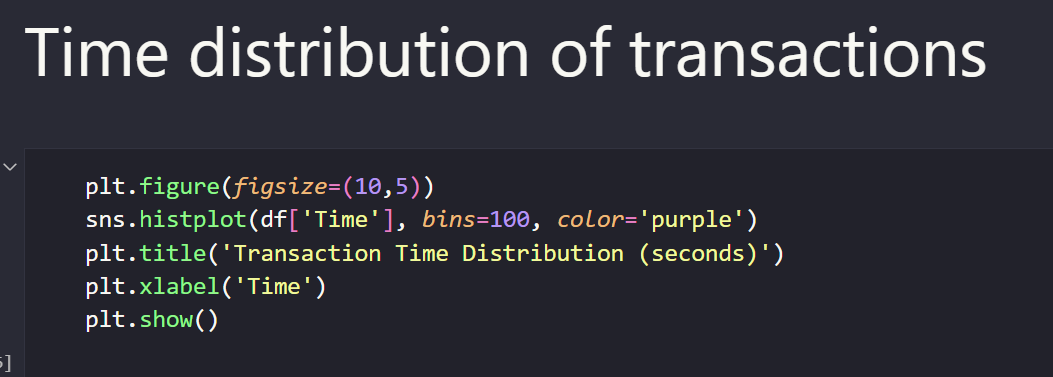
\includegraphics[width=468.00bp,height=167.55bp]{images/image_p27_18.png}};
  \node[anchor=north west,inner sep=0pt,outer sep=0pt] at (500.86,772.91) {{\fontsize{11.0bp}{13.2bp}\selectfont 19 | }};
  \node[anchor=north west,inner sep=0pt,outer sep=0pt] at (519.58,772.91) {{\fontsize{11.0bp}{13.2bp}\selectfont \textcolor{pdfcolor1}{P a g e}}};
  \node[anchor=north west,inner sep=0pt,outer sep=0pt] at (550.14,772.91) {{\fontsize{11.0bp}{13.2bp}\selectfont   }};
  \node[anchor=north west,inner sep=0pt,outer sep=0pt] at (70.82,407.99) {{\fontsize{13.9bp}{16.7bp}\selectfont \textbf{ 8. Time distribution of transactions: }}};
\end{tikzpicture}
\newpage
\noindent
\begin{tikzpicture}[x=1bp,y=-1bp,inner sep=0pt,outer sep=0pt]
  \useasboundingbox (0,0) rectangle (595.20,841.92);
  \fill[fill=pdfcolor9] (69.38,772.78) rectangle (554.40,773.26);
  \fill[fill=black] (70.82,395.40) rectangle (334.22,396.84);
  \node[anchor=north west,inner sep=0pt] at (70.90,85.05) {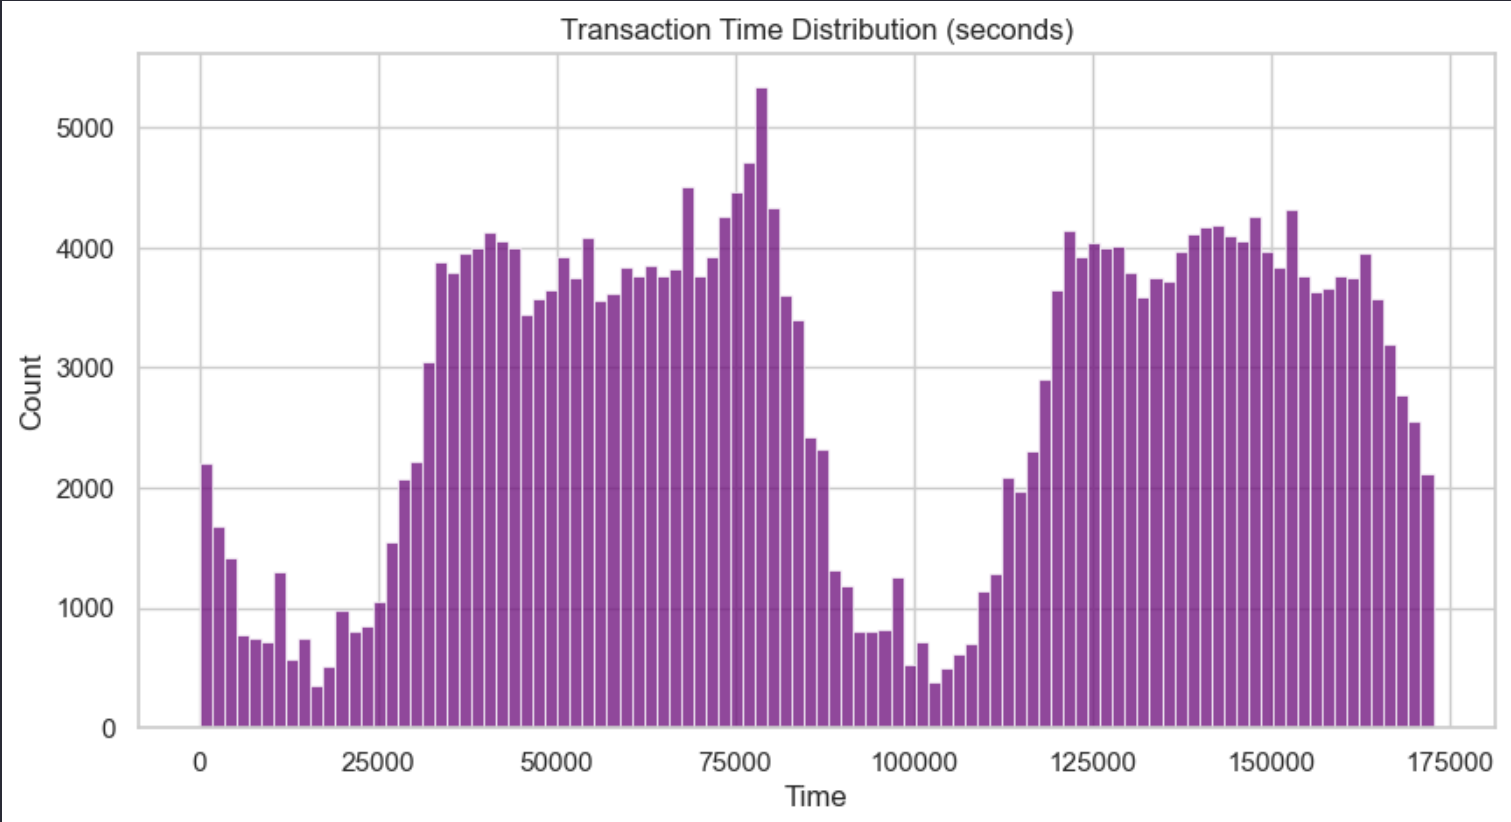
\includegraphics[width=468.00bp,height=254.60bp]{images/image_p28_19.png}};
  \node[anchor=north west,inner sep=0pt] at (70.90,438.01) {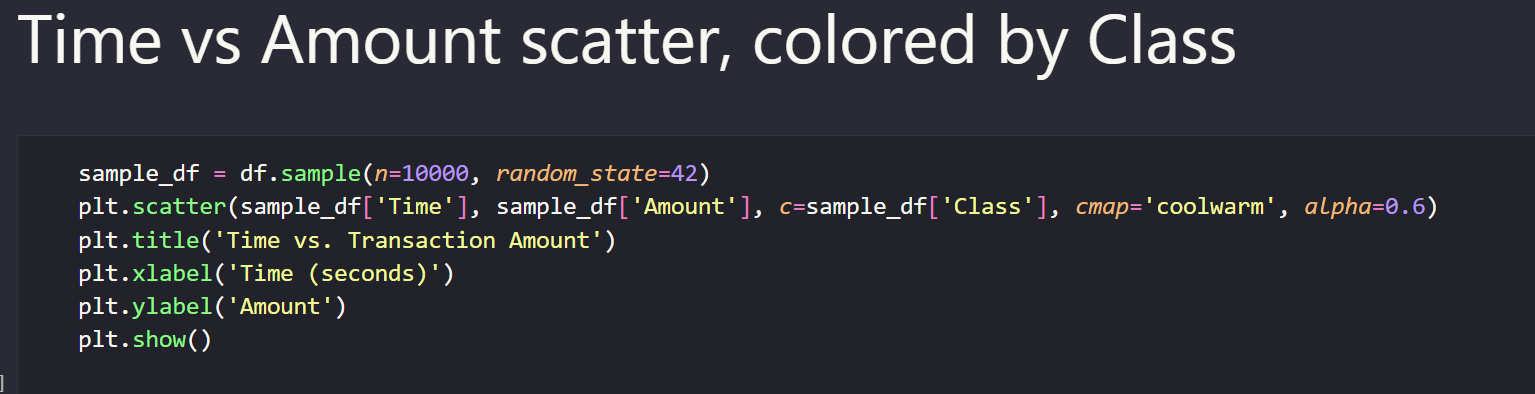
\includegraphics[width=468.00bp,height=120.10bp]{images/image_p28_20.png}};
  \node[anchor=north west,inner sep=0pt,outer sep=0pt] at (500.86,772.91) {{\fontsize{11.0bp}{13.2bp}\selectfont 20 | }};
  \node[anchor=north west,inner sep=0pt,outer sep=0pt] at (519.58,772.91) {{\fontsize{11.0bp}{13.2bp}\selectfont \textcolor{pdfcolor1}{P a g e}}};
  \node[anchor=north west,inner sep=0pt,outer sep=0pt] at (550.14,772.91) {{\fontsize{11.0bp}{13.2bp}\selectfont   }};
  \node[anchor=north west,inner sep=0pt,outer sep=0pt] at (70.82,379.43) {{\fontsize{13.9bp}{16.7bp}\selectfont \textbf{9. Time vs Amount scatter, colored by class: }}};
\end{tikzpicture}
\newpage
\noindent
\begin{tikzpicture}[x=1bp,y=-1bp,inner sep=0pt,outer sep=0pt]
  \useasboundingbox (0,0) rectangle (595.20,841.92);
  \fill[fill=pdfcolor9] (69.38,772.78) rectangle (554.40,773.26);
  \fill[fill=black] (70.82,431.40) rectangle (324.38,432.84);
  \node[anchor=north west,inner sep=0pt] at (70.90,85.05) {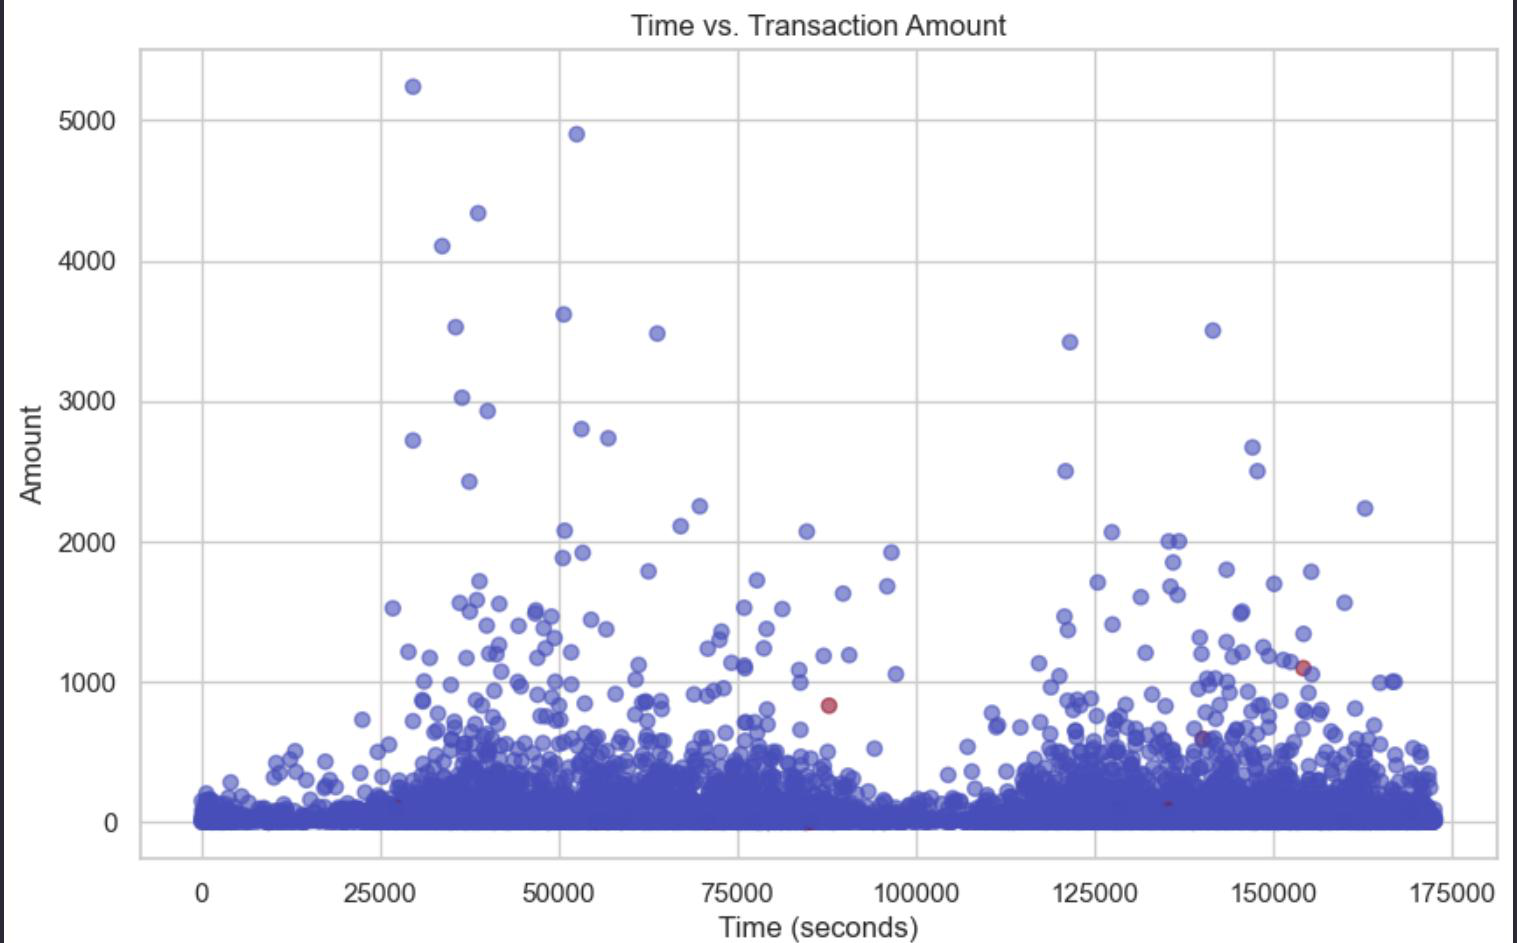
\includegraphics[width=468.00bp,height=290.90bp]{images/image_p29_21.png}};
  \node[anchor=north west,inner sep=0pt] at (70.90,474.01) {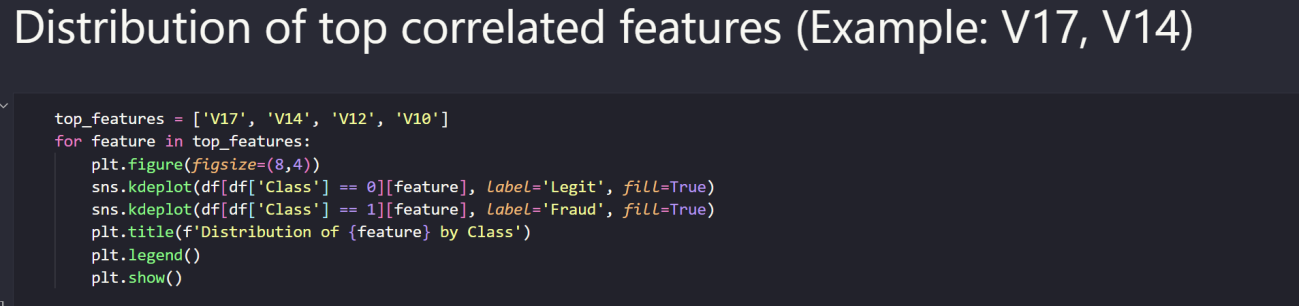
\includegraphics[width=468.00bp,height=110.20bp]{images/image_p29_22.png}};
  \node[anchor=north west,inner sep=0pt,outer sep=0pt] at (500.86,772.91) {{\fontsize{11.0bp}{13.2bp}\selectfont 21 | }};
  \node[anchor=north west,inner sep=0pt,outer sep=0pt] at (519.58,772.91) {{\fontsize{11.0bp}{13.2bp}\selectfont \textcolor{pdfcolor1}{P a g e}}};
  \node[anchor=north west,inner sep=0pt,outer sep=0pt] at (550.14,772.91) {{\fontsize{11.0bp}{13.2bp}\selectfont   }};
  \node[anchor=north west,inner sep=0pt,outer sep=0pt] at (70.82,415.43) {{\fontsize{13.9bp}{16.7bp}\selectfont \textbf{10. Distribution of top correlated features: }}};
\end{tikzpicture}
\newpage
\noindent
\begin{tikzpicture}[x=1bp,y=-1bp,inner sep=0pt,outer sep=0pt]
  \useasboundingbox (0,0) rectangle (595.20,841.92);
  \fill[fill=pdfcolor9] (69.38,772.78) rectangle (554.40,773.26);
  \node[anchor=north west,inner sep=0pt] at (70.90,85.05) {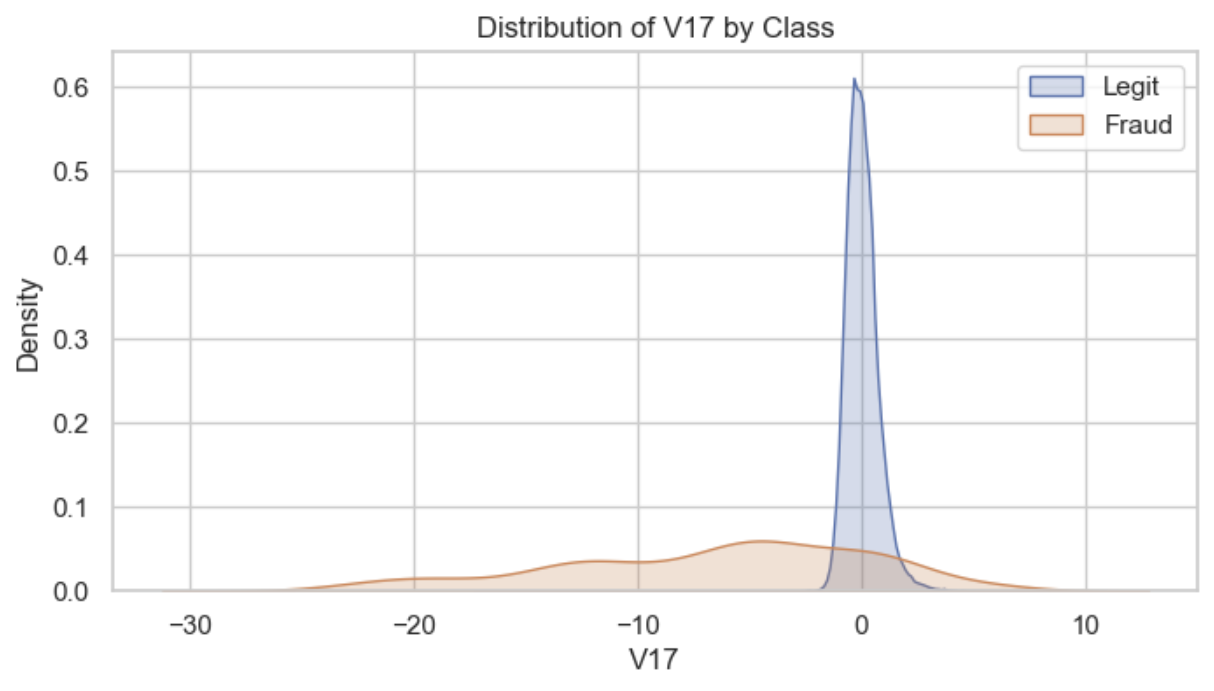
\includegraphics[width=468.00bp,height=266.40bp]{images/image_p30_23.png}};
  \node[anchor=north west,inner sep=0pt] at (70.90,352.05) {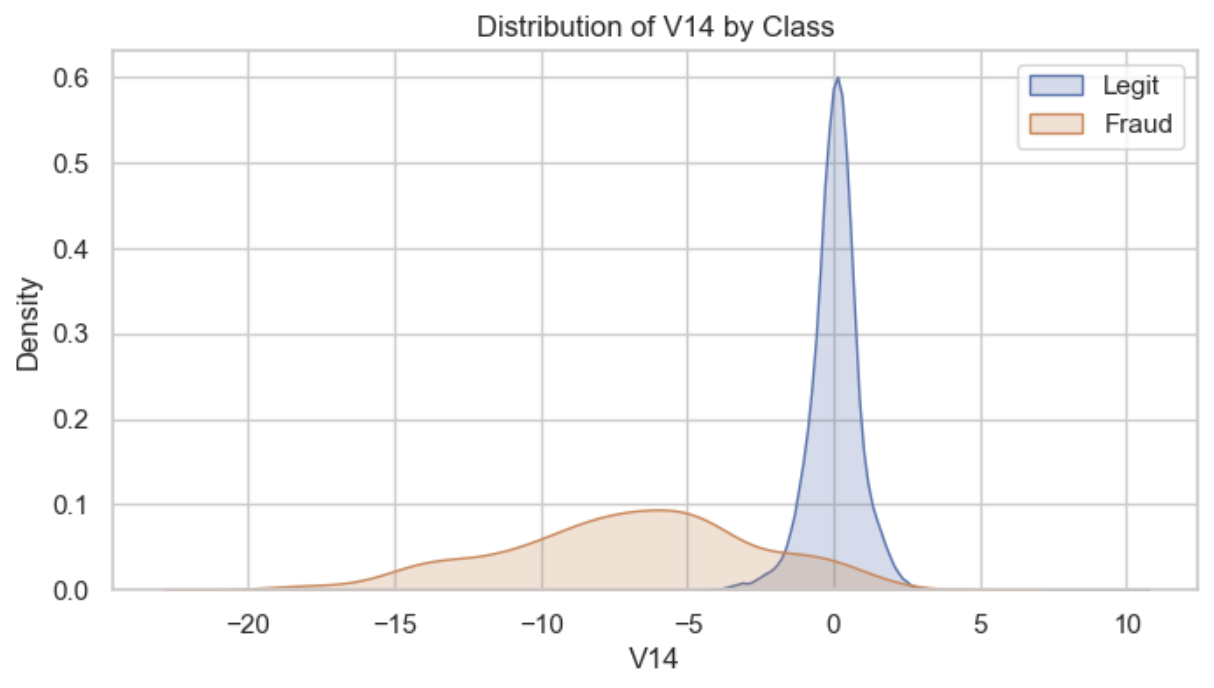
\includegraphics[width=468.00bp,height=265.20bp]{images/image_p30_24.png}};
  \node[anchor=north west,inner sep=0pt,outer sep=0pt] at (500.86,772.91) {{\fontsize{11.0bp}{13.2bp}\selectfont 22 | }};
  \node[anchor=north west,inner sep=0pt,outer sep=0pt] at (519.58,772.91) {{\fontsize{11.0bp}{13.2bp}\selectfont \textcolor{pdfcolor1}{P a g e}}};
  \node[anchor=north west,inner sep=0pt,outer sep=0pt] at (550.14,772.91) {{\fontsize{11.0bp}{13.2bp}\selectfont   }};
\end{tikzpicture}
\newpage
\noindent
\begin{tikzpicture}[x=1bp,y=-1bp,inner sep=0pt,outer sep=0pt]
  \useasboundingbox (0,0) rectangle (595.20,841.92);
  \fill[fill=pdfcolor9] (69.38,772.78) rectangle (554.40,773.26);
  \fill[fill=black] (70.82,642.67) rectangle (198.81,644.11);
  \node[anchor=north west,inner sep=0pt] at (70.90,85.05) {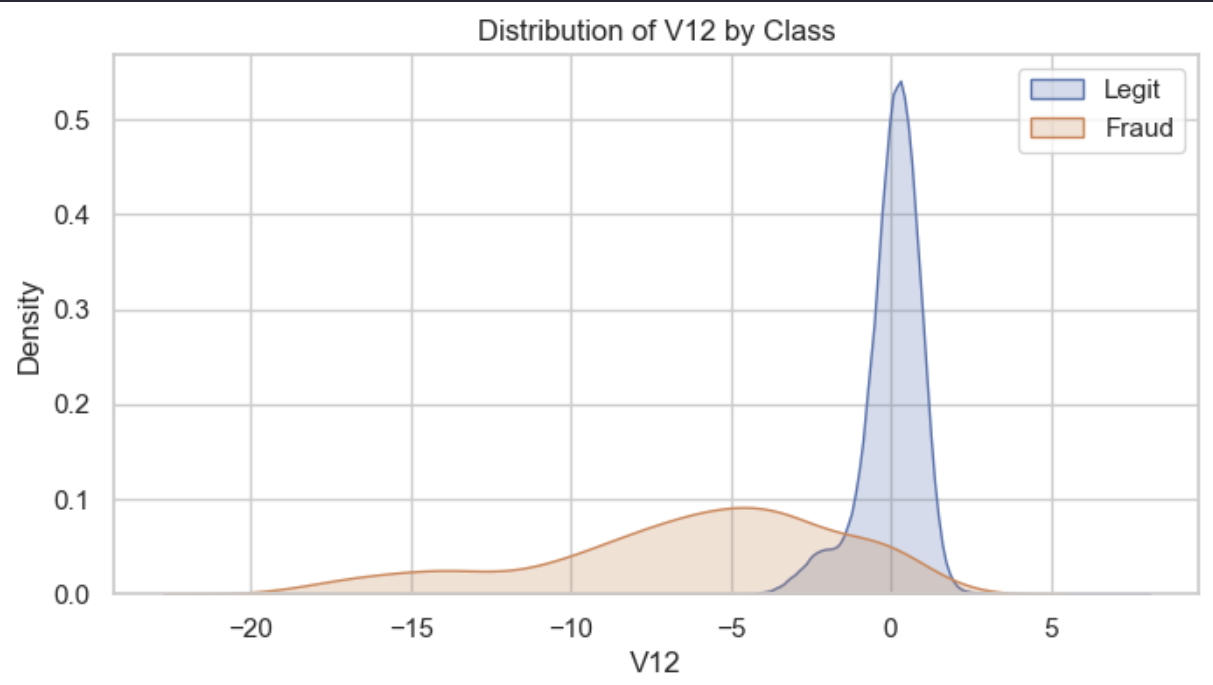
\includegraphics[width=455.91bp,height=257.60bp]{images/image_p31_25.png}};
  \node[anchor=north west,inner sep=0pt] at (70.90,355.46) {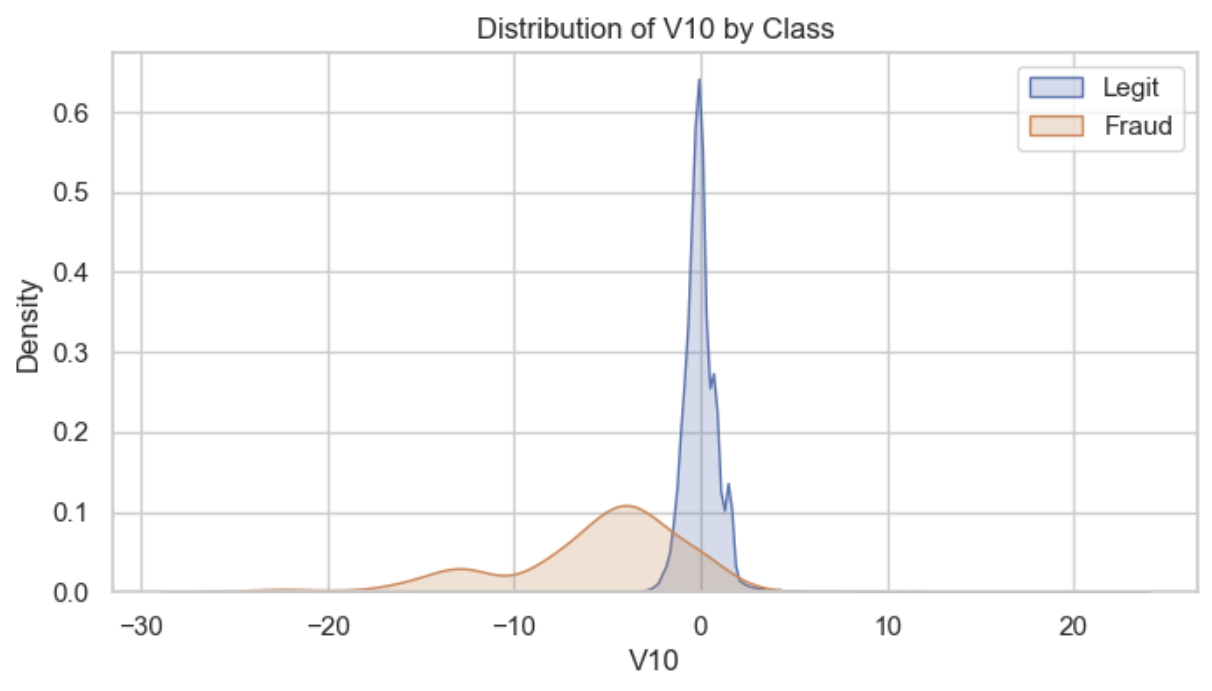
\includegraphics[width=456.40bp,height=260.19bp]{images/image_p31_26.png}};
  \node[anchor=north west,inner sep=0pt] at (70.90,656.59) {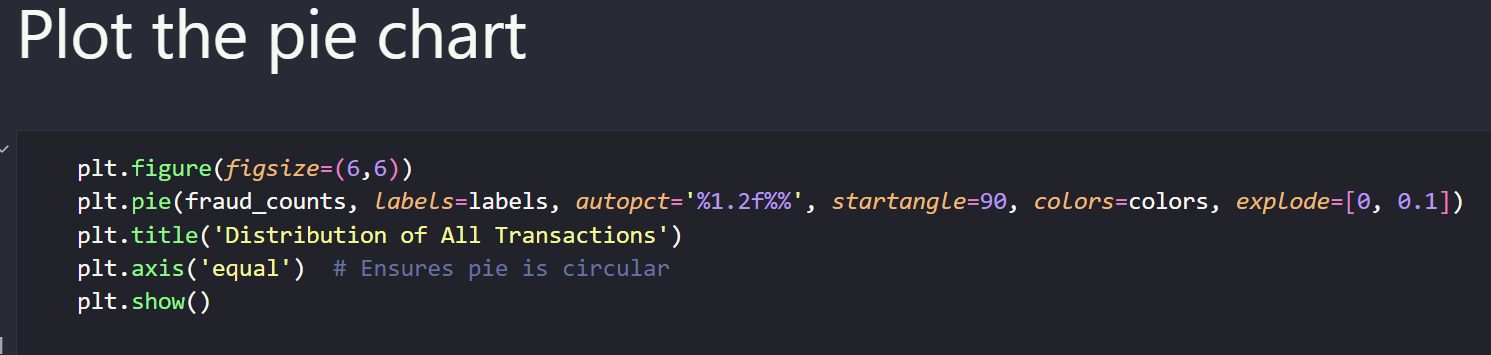
\includegraphics[width=453.70bp,height=108.00bp]{images/image_p31_27.png}};
  \node[anchor=north west,inner sep=0pt,outer sep=0pt] at (500.86,772.91) {{\fontsize{11.0bp}{13.2bp}\selectfont 23 | }};
  \node[anchor=north west,inner sep=0pt,outer sep=0pt] at (519.58,772.91) {{\fontsize{11.0bp}{13.2bp}\selectfont \textcolor{pdfcolor1}{P a g e}}};
  \node[anchor=north west,inner sep=0pt,outer sep=0pt] at (550.14,772.91) {{\fontsize{11.0bp}{13.2bp}\selectfont   }};
  \node[anchor=north west,inner sep=0pt,outer sep=0pt] at (70.82,626.68) {{\fontsize{13.9bp}{16.7bp}\selectfont \textbf{11. plot the pie chart: }}};
\end{tikzpicture}
\newpage
\noindent
\begin{tikzpicture}[x=1bp,y=-1bp,inner sep=0pt,outer sep=0pt]
  \useasboundingbox (0,0) rectangle (595.20,841.92);
  \fill[fill=pdfcolor9] (69.38,772.78) rectangle (554.40,773.26);
  \node[anchor=north west,inner sep=0pt] at (70.90,85.05) {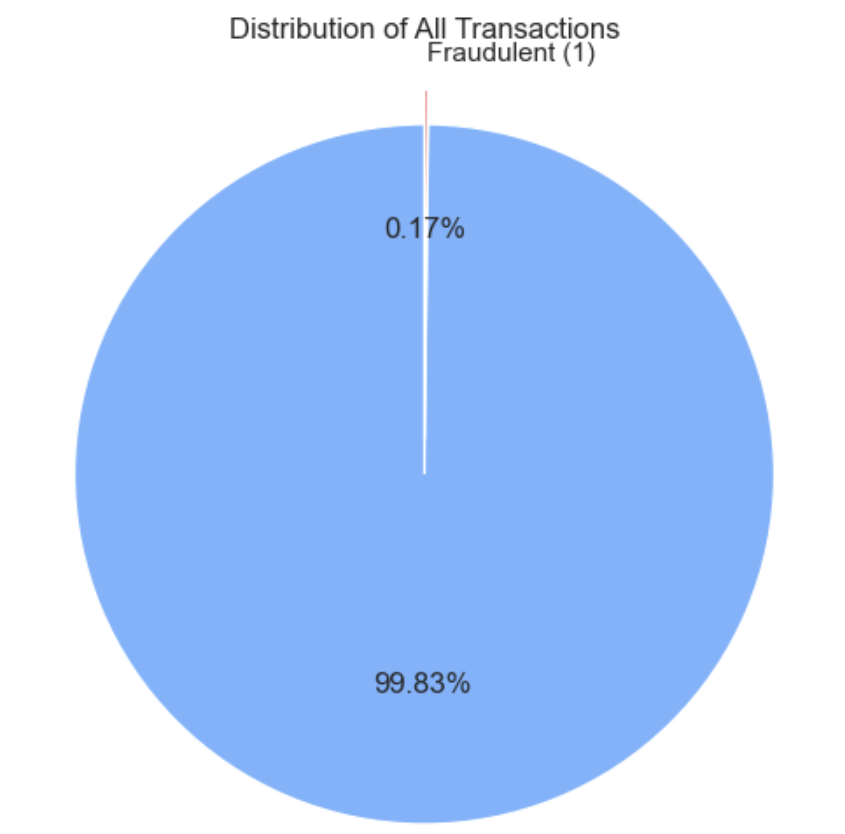
\includegraphics[width=469.37bp,height=463.25bp]{images/image_p32_28.png}};
  \node[anchor=north west,inner sep=0pt] at (70.90,589.48) {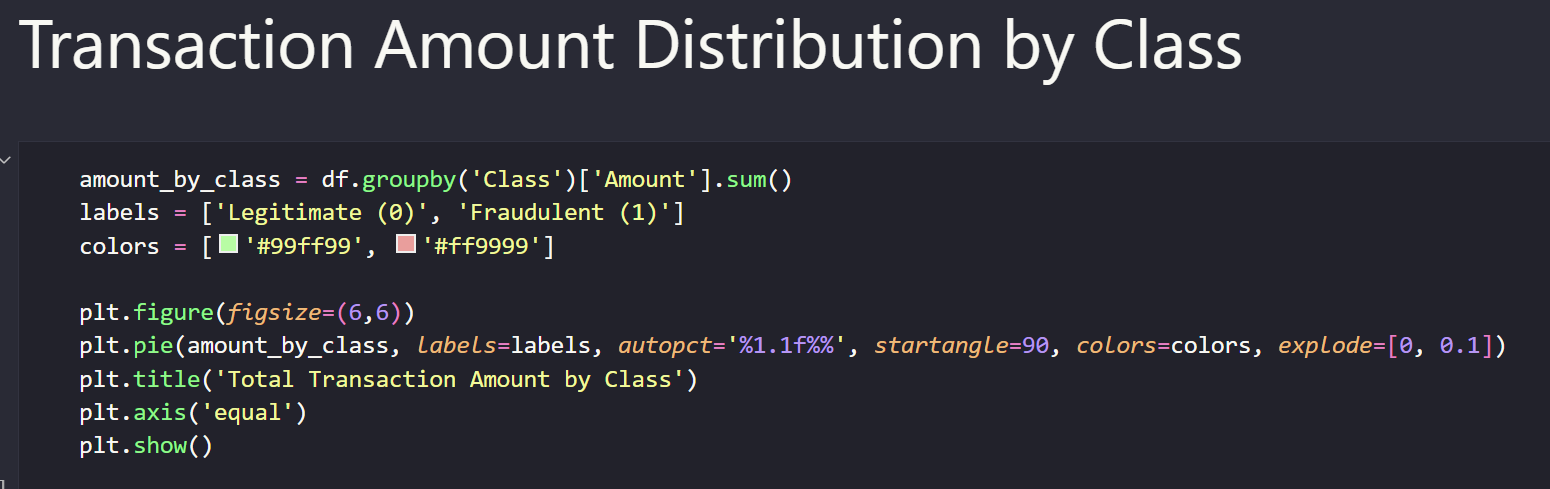
\includegraphics[width=468.00bp,height=147.65bp]{images/image_p32_29.png}};
  \node[anchor=north west,inner sep=0pt,outer sep=0pt] at (500.86,772.91) {{\fontsize{11.0bp}{13.2bp}\selectfont 24 | }};
  \node[anchor=north west,inner sep=0pt,outer sep=0pt] at (519.58,772.91) {{\fontsize{11.0bp}{13.2bp}\selectfont \textcolor{pdfcolor1}{P a g e}}};
  \node[anchor=north west,inner sep=0pt,outer sep=0pt] at (550.14,772.91) {{\fontsize{11.0bp}{13.2bp}\selectfont   }};
\end{tikzpicture}
\newpage
\noindent
\begin{tikzpicture}[x=1bp,y=-1bp,inner sep=0pt,outer sep=0pt]
  \useasboundingbox (0,0) rectangle (595.20,841.92);
  \fill[fill=pdfcolor9] (69.38,772.78) rectangle (554.40,773.26);
  \node[anchor=north west,inner sep=0pt] at (70.90,85.05) {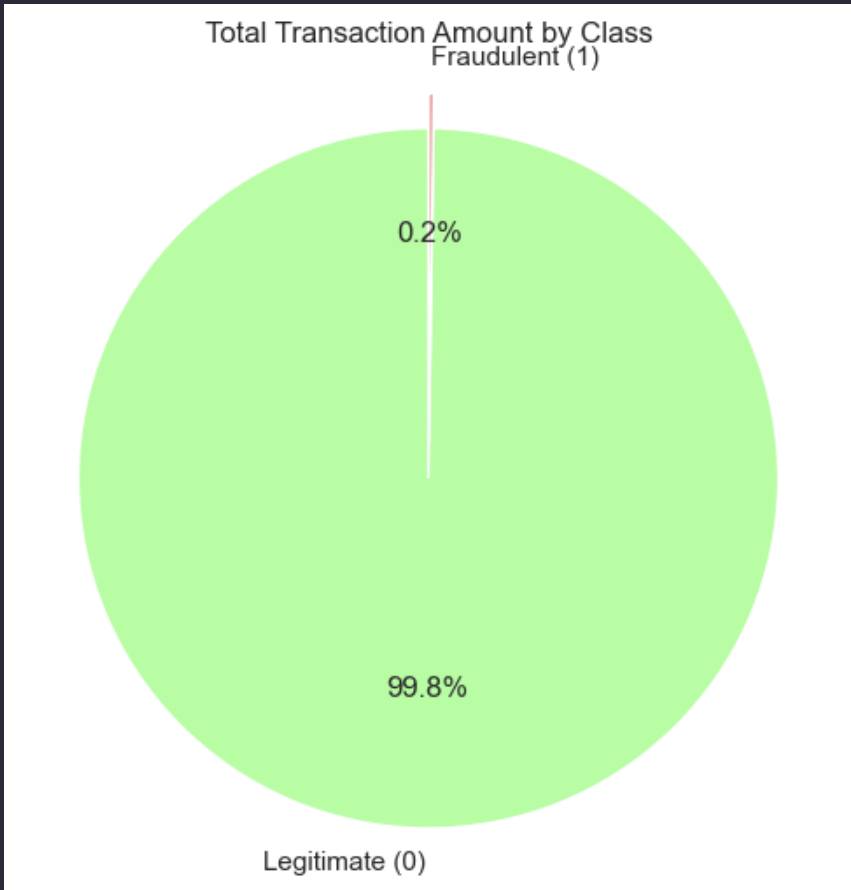
\includegraphics[width=468.00bp,height=489.45bp]{images/image_p33_30.png}};
  \node[anchor=north west,inner sep=0pt,outer sep=0pt] at (500.86,772.91) {{\fontsize{11.0bp}{13.2bp}\selectfont 25 | }};
  \node[anchor=north west,inner sep=0pt,outer sep=0pt] at (519.58,772.91) {{\fontsize{11.0bp}{13.2bp}\selectfont \textcolor{pdfcolor1}{P a g e}}};
  \node[anchor=north west,inner sep=0pt,outer sep=0pt] at (550.14,772.91) {{\fontsize{11.0bp}{13.2bp}\selectfont   }};
\end{tikzpicture}
\newpage
\noindent
\begin{tikzpicture}[x=1bp,y=-1bp,inner sep=0pt,outer sep=0pt]
  \useasboundingbox (0,0) rectangle (595.20,841.92);
  \fill[fill=pdfcolor9] (69.38,772.78) rectangle (554.40,773.26);
  \node[anchor=north west,inner sep=0pt] at (70.90,85.05) {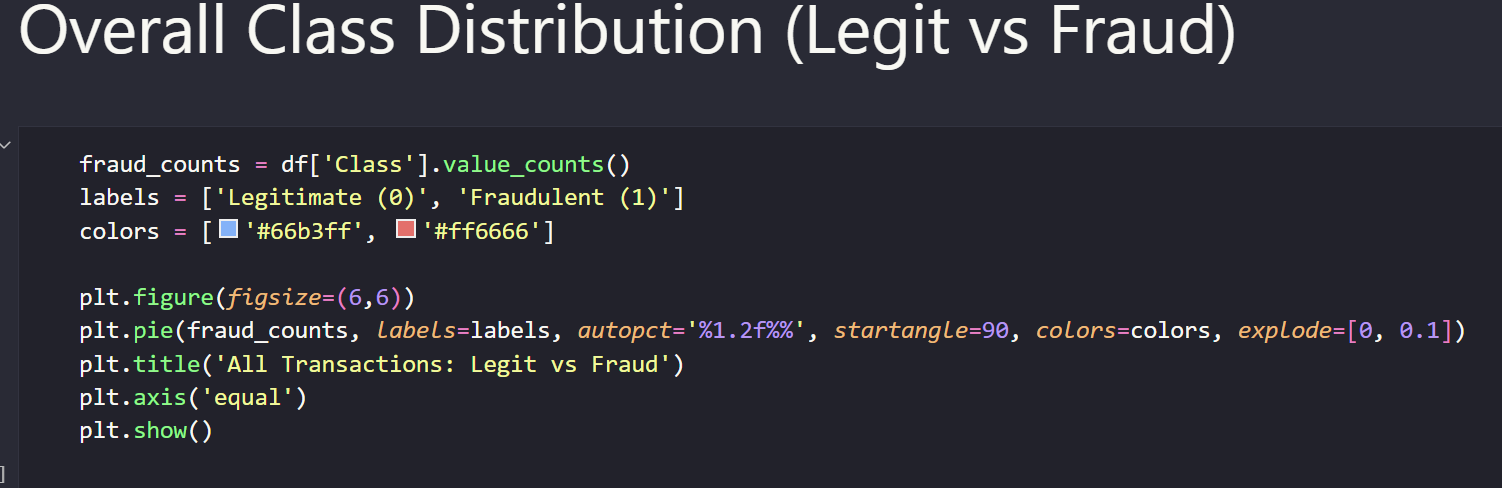
\includegraphics[width=468.00bp,height=152.05bp]{images/image_p34_31.png}};
  \node[anchor=north west,inner sep=0pt] at (70.90,237.10) {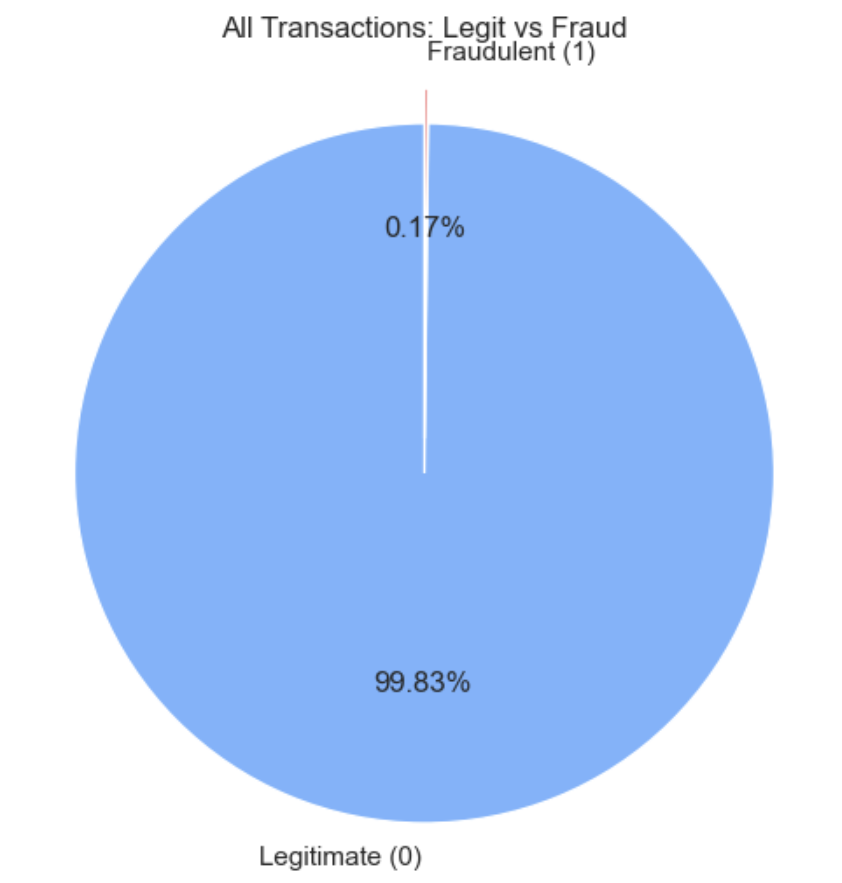
\includegraphics[width=468.00bp,height=490.80bp]{images/image_p34_32.png}};
  \node[anchor=north west,inner sep=0pt,outer sep=0pt] at (500.86,772.91) {{\fontsize{11.0bp}{13.2bp}\selectfont 26 | }};
  \node[anchor=north west,inner sep=0pt,outer sep=0pt] at (519.58,772.91) {{\fontsize{11.0bp}{13.2bp}\selectfont \textcolor{pdfcolor1}{P a g e}}};
  \node[anchor=north west,inner sep=0pt,outer sep=0pt] at (550.14,772.91) {{\fontsize{11.0bp}{13.2bp}\selectfont   }};
\end{tikzpicture}
\newpage
\noindent
\begin{tikzpicture}[x=1bp,y=-1bp,inner sep=0pt,outer sep=0pt]
  \useasboundingbox (0,0) rectangle (595.20,841.92);
  \fill[fill=pdfcolor9] (69.38,772.78) rectangle (554.40,773.26);
  \node[anchor=north west,inner sep=0pt] at (70.90,85.05) {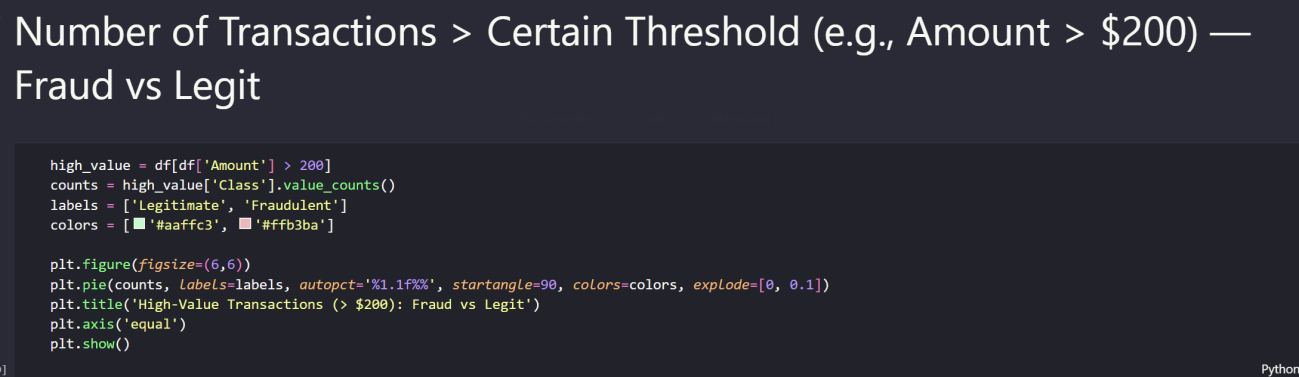
\includegraphics[width=468.00bp,height=135.85bp]{images/image_p35_33.png}};
  \node[anchor=north west,inner sep=0pt] at (70.90,221.55) {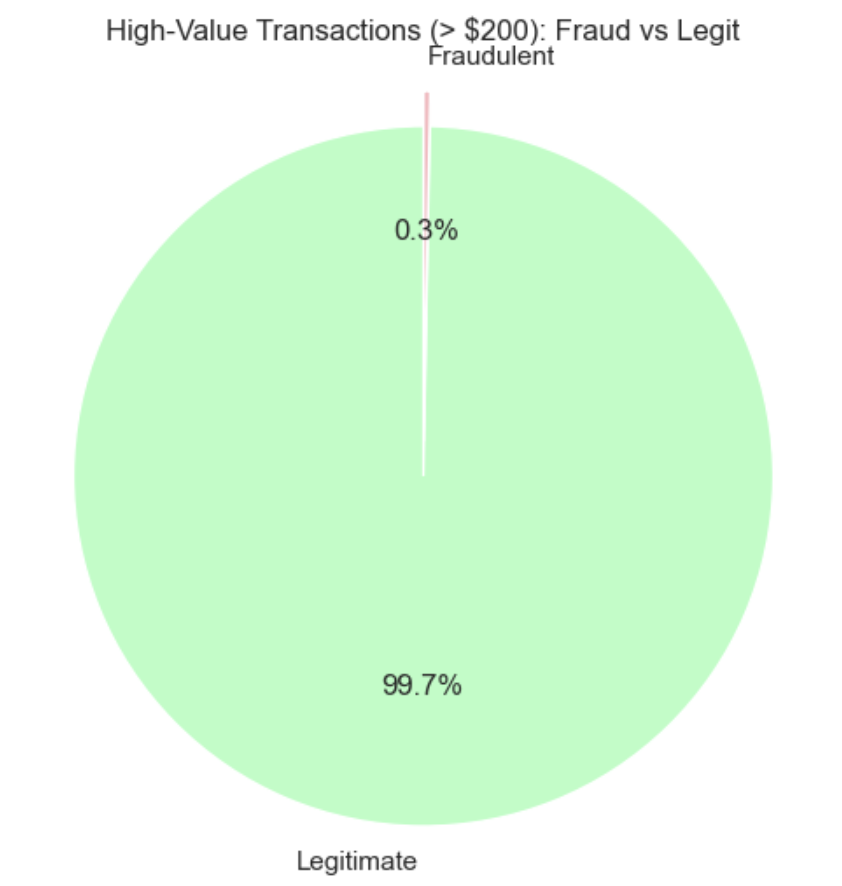
\includegraphics[width=468.00bp,height=492.45bp]{images/image_p35_34.png}};
  \node[anchor=north west,inner sep=0pt,outer sep=0pt] at (500.86,772.91) {{\fontsize{11.0bp}{13.2bp}\selectfont 27 | }};
  \node[anchor=north west,inner sep=0pt,outer sep=0pt] at (519.58,772.91) {{\fontsize{11.0bp}{13.2bp}\selectfont \textcolor{pdfcolor1}{P a g e}}};
  \node[anchor=north west,inner sep=0pt,outer sep=0pt] at (550.14,772.91) {{\fontsize{11.0bp}{13.2bp}\selectfont   }};
\end{tikzpicture}
\newpage
\noindent
\begin{tikzpicture}[x=1bp,y=-1bp,inner sep=0pt,outer sep=0pt]
  \useasboundingbox (0,0) rectangle (595.20,841.92);
  \fill[fill=pdfcolor9] (69.38,772.78) rectangle (554.40,773.26);
  \fill[fill=black] (70.82,99.38) rectangle (264.12,100.82);
  \node[anchor=north west,inner sep=0pt] at (70.90,142.07) {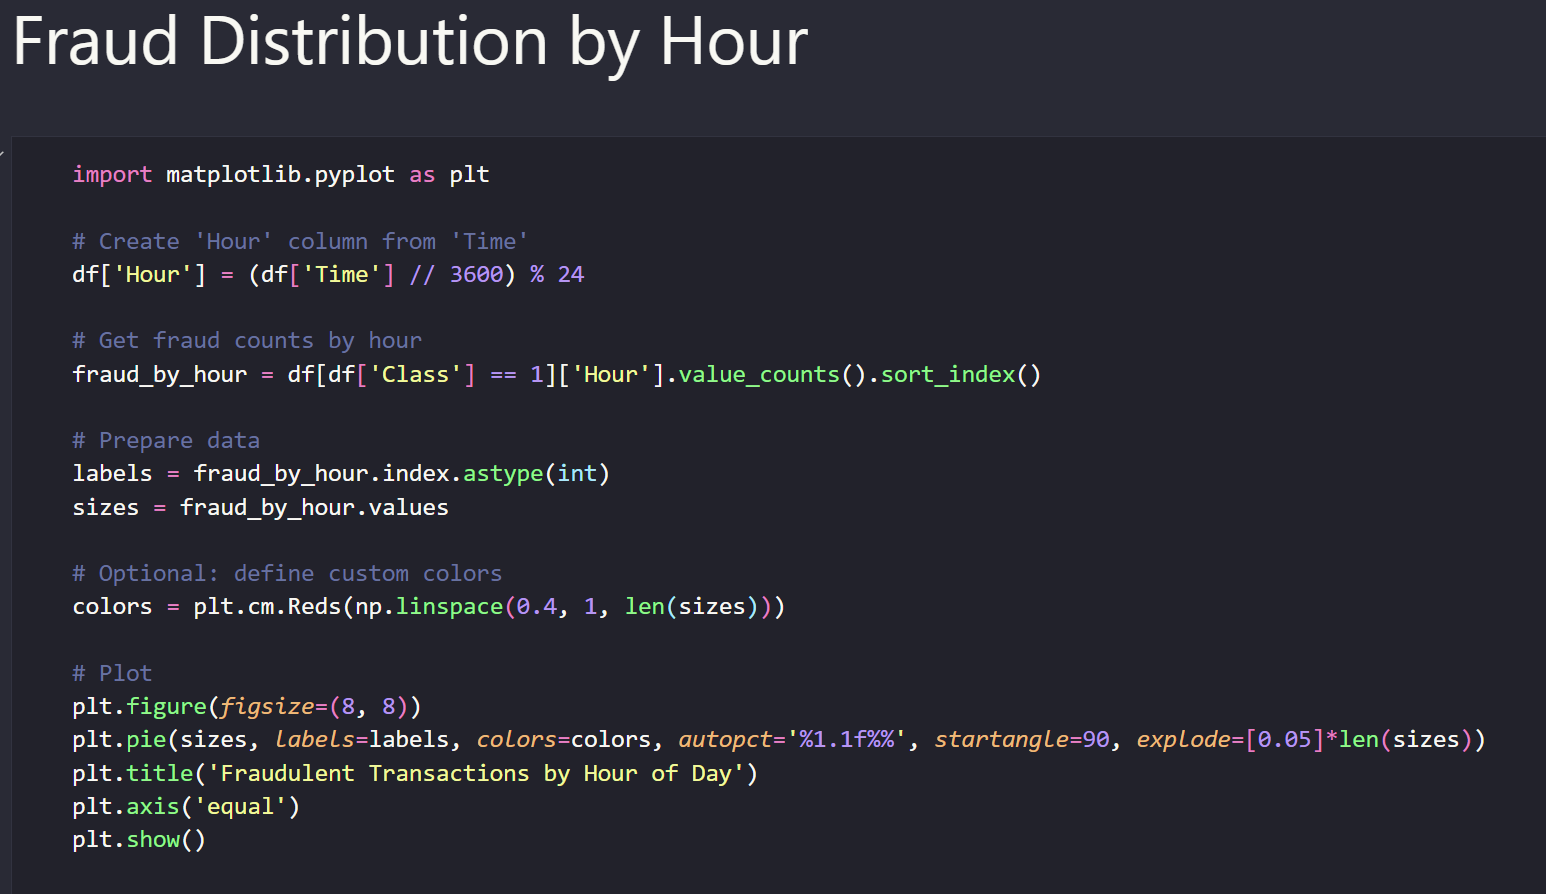
\includegraphics[width=446.10bp,height=257.94bp]{images/image_p36_35.png}};
  \node[anchor=north west,inner sep=0pt] at (70.90,412.49) {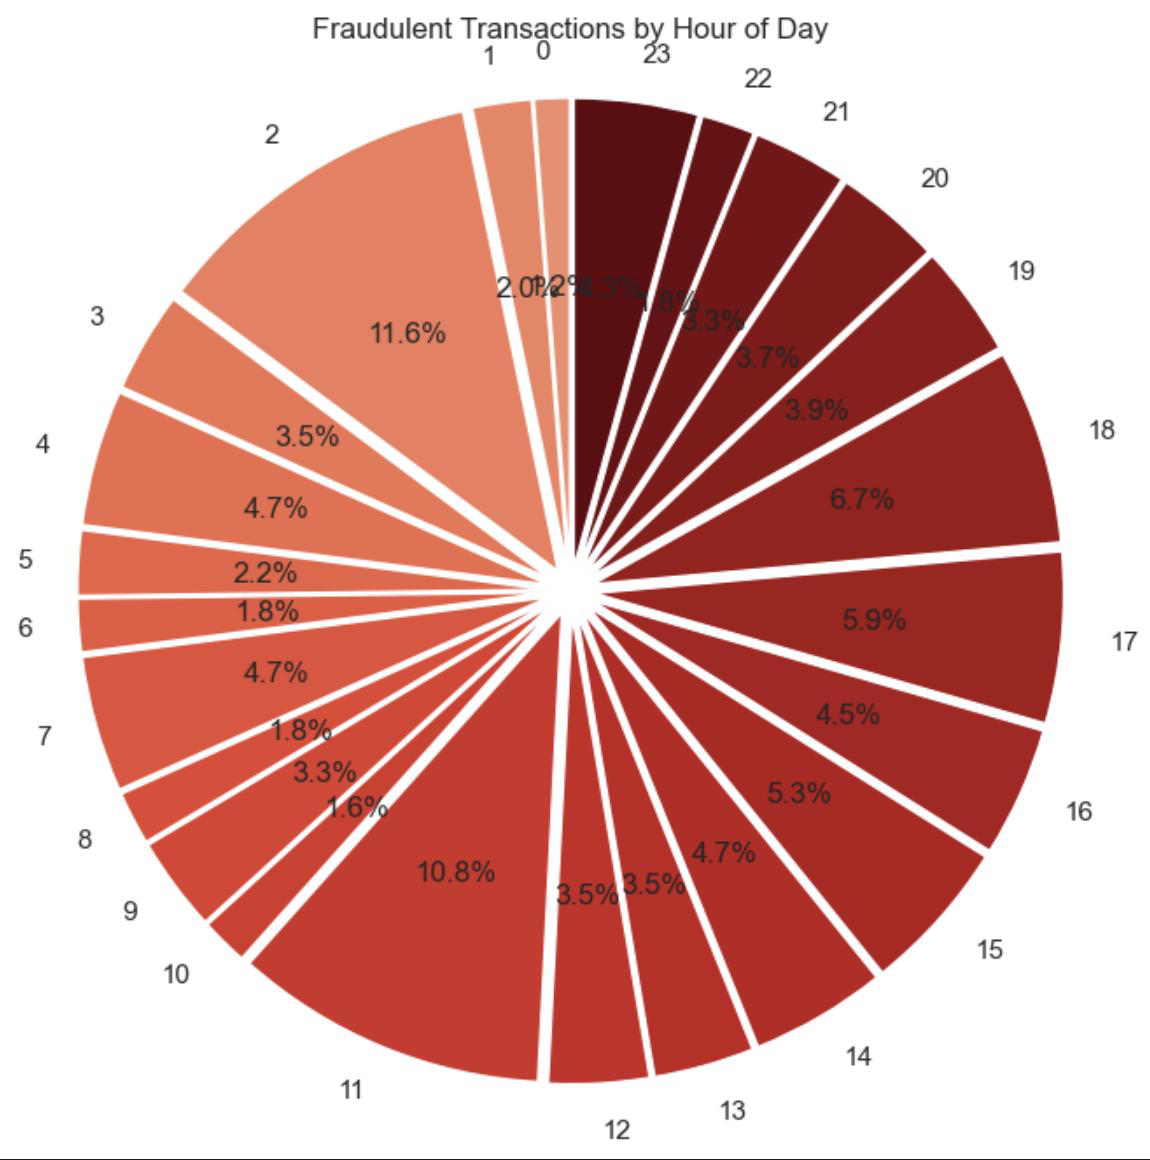
\includegraphics[width=354.38bp,height=357.45bp]{images/image_p36_36.png}};
  \node[anchor=north west,inner sep=0pt,outer sep=0pt] at (500.86,772.91) {{\fontsize{11.0bp}{13.2bp}\selectfont 28 | }};
  \node[anchor=north west,inner sep=0pt,outer sep=0pt] at (519.58,772.91) {{\fontsize{11.0bp}{13.2bp}\selectfont \textcolor{pdfcolor1}{P a g e}}};
  \node[anchor=north west,inner sep=0pt,outer sep=0pt] at (550.14,772.91) {{\fontsize{11.0bp}{13.2bp}\selectfont   }};
  \node[anchor=north west,inner sep=0pt,outer sep=0pt] at (70.82,83.41) {{\fontsize{13.9bp}{16.7bp}\selectfont \textbf{12. Fraud Distribution by Hour: }}};
\end{tikzpicture}
\newpage
\noindent

\begin{tikzpicture}[x=1bp,y=-1bp,inner sep=0pt,outer sep=0pt]
  \useasboundingbox (0,0) rectangle (595.20,841.92);
  \fill[fill=pdfcolor9] (69.38,772.78) rectangle (554.40,773.26);
  \fill[fill=black] (142.87,101.78) rectangle (450.91,103.22);
  \node[anchor=north west,inner sep=0pt,outer sep=0pt] at (500.86,772.91) {{\fontsize{11.0bp}{13.2bp}\selectfont 29 | }};
  \node[anchor=north west,inner sep=0pt,outer sep=0pt] at (519.58,772.91) {{\fontsize{11.0bp}{13.2bp}\selectfont \textcolor{pdfcolor1}{P a g e}}};
  \node[anchor=north west,inner sep=0pt,outer sep=0pt] at (550.14,772.91) {{\fontsize{11.0bp}{13.2bp}\selectfont   }};
  \node[anchor=north west,inner sep=0pt,outer sep=0pt] at (142.87,83.31) {{\fontsize{16.1bp}{19.3bp}\selectfont \textbf{3.}}};
  \node[anchor=north west,inner sep=0pt,outer sep=0pt] at (155.11,85.57) {{\fontsize{13.9bp}{16.7bp}\selectfont \textbf{ }}};
  \node[anchor=north west,inner sep=0pt,outer sep=0pt] at (158.71,83.31) {{\fontsize{16.1bp}{19.3bp}\selectfont \textbf{SYSTEM IMPLIMENTATION DETAILS}}};
  \node[anchor=north west,inner sep=0pt,outer sep=0pt] at (450.91,88.47) {{\fontsize{11.0bp}{13.2bp}\selectfont  }};
  \node[anchor=north west,inner sep=0pt,outer sep=0pt] at (80.90,114.61) {{\fontsize{12.0bp}{14.4bp}\selectfont This section details the step-by-step implementation of the Credit Card Fraud Detection System, }};
  \node[anchor=north west,inner sep=0pt,outer sep=0pt] at (106.85,128.53) {{\fontsize{12.0bp}{14.4bp}\selectfont elaborating on the applied methodology, technology stack, and essential source code }};
  \node[anchor=north west,inner sep=0pt,outer sep=0pt] at (106.85,142.21) {{\fontsize{12.0bp}{14.4bp}\selectfont integrations. }};
  \node[anchor=north west,inner sep=0pt,outer sep=0pt] at (80.90,183.84) {{\fontsize{12.0bp}{14.4bp}\selectfont \textbf{3.1 Methodology Adopted }}};
  \node[anchor=north west,inner sep=0pt,outer sep=0pt] at (80.90,204.39) {{\fontsize{12.0bp}{14.4bp}\selectfont To ensure accuracy and adaptability in fraud detection, the project applies a structured, data-}};
  \node[anchor=north west,inner sep=0pt,outer sep=0pt] at (106.85,218.07) {{\fontsize{12.0bp}{14.4bp}\selectfont driven machine learning methodology. The approach is modular, ensuring that each }};
  \node[anchor=north west,inner sep=0pt,outer sep=0pt] at (106.85,231.75) {{\fontsize{12.0bp}{14.4bp}\selectfont component---from preprocessing to deployment---can be individually developed, tested, and }};
  \node[anchor=north west,inner sep=0pt,outer sep=0pt] at (106.85,245.67) {{\fontsize{12.0bp}{14.4bp}\selectfont maintained. Below are the primary stages involved: }};
  \node[anchor=north west,inner sep=0pt,outer sep=0pt] at (88.85,266.31) {{\fontsize{12.0bp}{14.4bp}\selectfont 1.}};
  \node[anchor=north west,inner sep=0pt,outer sep=0pt] at (97.97,266.05) {\textsf{{\fontsize{12.0bp}{14.4bp}\selectfont  }}};
  \node[anchor=north west,inner sep=0pt,outer sep=0pt] at (106.85,266.42) {{\fontsize{12.0bp}{14.4bp}\selectfont \textbf{Data Collection:}}};
  \node[anchor=north west,inner sep=0pt,outer sep=0pt] at (190.63,266.31) {{\fontsize{12.0bp}{14.4bp}\selectfont  The Kaggle Credit Card Fraud Detection dataset is utilized, which }};
  \node[anchor=north west,inner sep=0pt,outer sep=0pt] at (106.85,279.99) {{\fontsize{12.0bp}{14.4bp}\selectfont contains anonymized features derived through PCA, along with 'Time', 'Amount', and a }};
  \node[anchor=north west,inner sep=0pt,outer sep=0pt] at (106.85,293.94) {{\fontsize{12.0bp}{14.4bp}\selectfont 'Class' label. }};
  \node[anchor=north west,inner sep=0pt,outer sep=0pt] at (88.85,314.69) {{\fontsize{12.0bp}{14.4bp}\selectfont \textbf{2.}}};
  \node[anchor=north west,inner sep=0pt,outer sep=0pt] at (97.97,314.38) {\textsf{{\fontsize{12.0bp}{14.4bp}\selectfont \textbf{ }}}};
  \node[anchor=north west,inner sep=0pt,outer sep=0pt] at (106.85,314.69) {{\fontsize{12.0bp}{14.4bp}\selectfont \textbf{Preprocessing: }}};
  \node[anchor=north west,inner sep=0pt,outer sep=0pt] at (124.85,339.47) {\texttt{{\fontsize{10.1bp}{12.1bp}\selectfont o}}};
  \node[anchor=north west,inner sep=0pt,outer sep=0pt] at (130.85,337.02) {\textsf{{\fontsize{10.1bp}{12.1bp}\selectfont  }}};
  \node[anchor=north west,inner sep=0pt,outer sep=0pt] at (142.87,335.22) {{\fontsize{12.0bp}{14.4bp}\selectfont Feature Scaling: Time and Amount are normalized using StandardScaler to ensure }};
  \node[anchor=north west,inner sep=0pt,outer sep=0pt] at (142.87,348.90) {{\fontsize{12.0bp}{14.4bp}\selectfont uniformity. }};
  \node[anchor=north west,inner sep=0pt,outer sep=0pt] at (124.85,374.03) {\texttt{{\fontsize{10.1bp}{12.1bp}\selectfont o}}};
  \node[anchor=north west,inner sep=0pt,outer sep=0pt] at (130.85,371.58) {\textsf{{\fontsize{10.1bp}{12.1bp}\selectfont  }}};
  \node[anchor=north west,inner sep=0pt,outer sep=0pt] at (142.87,369.78) {{\fontsize{12.0bp}{14.4bp}\selectfont Class Balancing: The dataset’s high imbalance (fraud cases <1\%) is handled using }};
  \node[anchor=north west,inner sep=0pt,outer sep=0pt] at (142.87,383.48) {{\fontsize{12.0bp}{14.4bp}\selectfont SMOTE, which synthetically creates samples of the minority class. }};
  \node[anchor=north west,inner sep=0pt,outer sep=0pt] at (88.85,404.23) {{\fontsize{12.0bp}{14.4bp}\selectfont \textbf{3.}}};
  \node[anchor=north west,inner sep=0pt,outer sep=0pt] at (97.97,403.92) {\textsf{{\fontsize{12.0bp}{14.4bp}\selectfont \textbf{ }}}};
  \node[anchor=north west,inner sep=0pt,outer sep=0pt] at (106.85,404.23) {{\fontsize{12.0bp}{14.4bp}\selectfont \textbf{Model Training: }}};
  \node[anchor=north west,inner sep=0pt,outer sep=0pt] at (124.85,429.01) {\texttt{{\fontsize{10.1bp}{12.1bp}\selectfont o}}};
  \node[anchor=north west,inner sep=0pt,outer sep=0pt] at (130.85,426.56) {\textsf{{\fontsize{10.1bp}{12.1bp}\selectfont  }}};
  \node[anchor=north west,inner sep=0pt,outer sep=0pt] at (142.87,424.76) {{\fontsize{12.0bp}{14.4bp}\selectfont A RandomForestClassifier is selected for its accuracy and robustness. }};
  \node[anchor=north west,inner sep=0pt,outer sep=0pt] at (124.85,449.65) {\texttt{{\fontsize{10.1bp}{12.1bp}\selectfont o}}};
  \node[anchor=north west,inner sep=0pt,outer sep=0pt] at (130.85,447.20) {\textsf{{\fontsize{10.1bp}{12.1bp}\selectfont  }}};
  \node[anchor=north west,inner sep=0pt,outer sep=0pt] at (142.87,445.40) {{\fontsize{12.0bp}{14.4bp}\selectfont The model is trained using a stratified train-test split to preserve class distribution. }};
  \node[anchor=north west,inner sep=0pt,outer sep=0pt] at (124.85,470.55) {\texttt{{\fontsize{10.1bp}{12.1bp}\selectfont o}}};
  \node[anchor=north west,inner sep=0pt,outer sep=0pt] at (130.85,468.10) {\textsf{{\fontsize{10.1bp}{12.1bp}\selectfont  }}};
  \node[anchor=north west,inner sep=0pt,outer sep=0pt] at (142.87,466.30) {{\fontsize{12.0bp}{14.4bp}\selectfont The trained model is saved using joblib for deployment. }};
  \node[anchor=north west,inner sep=0pt,outer sep=0pt] at (88.85,487.05) {{\fontsize{12.0bp}{14.4bp}\selectfont \textbf{4.}}};
  \node[anchor=north west,inner sep=0pt,outer sep=0pt] at (97.97,486.74) {\textsf{{\fontsize{12.0bp}{14.4bp}\selectfont \textbf{ }}}};
  \node[anchor=north west,inner sep=0pt,outer sep=0pt] at (106.85,487.05) {{\fontsize{12.0bp}{14.4bp}\selectfont \textbf{Model Evaluation: }}};
  \node[anchor=north west,inner sep=0pt,outer sep=0pt] at (124.85,511.83) {\texttt{{\fontsize{10.1bp}{12.1bp}\selectfont o}}};
  \node[anchor=north west,inner sep=0pt,outer sep=0pt] at (130.85,509.38) {\textsf{{\fontsize{10.1bp}{12.1bp}\selectfont  }}};
  \node[anchor=north west,inner sep=0pt,outer sep=0pt] at (142.87,507.58) {{\fontsize{12.0bp}{14.4bp}\selectfont Accuracy alone is not sufficient; thus, evaluation metrics such as F1-score, Recall, }};
  \node[anchor=north west,inner sep=0pt,outer sep=0pt] at (142.87,521.26) {{\fontsize{12.0bp}{14.4bp}\selectfont Precision, and ROC-AUC are used. }};
  \node[anchor=north west,inner sep=0pt,outer sep=0pt] at (124.85,546.15) {\texttt{{\fontsize{10.1bp}{12.1bp}\selectfont o}}};
  \node[anchor=north west,inner sep=0pt,outer sep=0pt] at (130.85,543.70) {\textsf{{\fontsize{10.1bp}{12.1bp}\selectfont  }}};
  \node[anchor=north west,inner sep=0pt,outer sep=0pt] at (142.87,541.90) {{\fontsize{12.0bp}{14.4bp}\selectfont Confusion matrix and ROC curve visualizations help validate the model's }};
  \node[anchor=north west,inner sep=0pt,outer sep=0pt] at (142.87,555.61) {{\fontsize{12.0bp}{14.4bp}\selectfont performance on imbalanced data. }};
  \node[anchor=north west,inner sep=0pt,outer sep=0pt] at (88.85,576.60) {{\fontsize{12.0bp}{14.4bp}\selectfont \textbf{5.}}};
  \node[anchor=north west,inner sep=0pt,outer sep=0pt] at (97.97,576.29) {\textsf{{\fontsize{12.0bp}{14.4bp}\selectfont \textbf{ }}}};
  \node[anchor=north west,inner sep=0pt,outer sep=0pt] at (106.85,576.60) {{\fontsize{12.0bp}{14.4bp}\selectfont \textbf{Model Deployment: }}};
  \node[anchor=north west,inner sep=0pt,outer sep=0pt] at (124.85,601.38) {\texttt{{\fontsize{10.1bp}{12.1bp}\selectfont o}}};
  \node[anchor=north west,inner sep=0pt,outer sep=0pt] at (130.85,598.93) {\textsf{{\fontsize{10.1bp}{12.1bp}\selectfont  }}};
  \node[anchor=north west,inner sep=0pt,outer sep=0pt] at (142.87,597.13) {{\fontsize{12.0bp}{14.4bp}\selectfont Streamlit, a Python-based UI framework, is used to deploy the model. }};
  \node[anchor=north west,inner sep=0pt,outer sep=0pt] at (124.85,622.02) {\texttt{{\fontsize{10.1bp}{12.1bp}\selectfont o}}};
  \node[anchor=north west,inner sep=0pt,outer sep=0pt] at (130.85,619.57) {\textsf{{\fontsize{10.1bp}{12.1bp}\selectfont  }}};
  \node[anchor=north west,inner sep=0pt,outer sep=0pt] at (142.87,617.77) {{\fontsize{12.0bp}{14.4bp}\selectfont A responsive and simple interface allows users to manually input transaction }};
  \node[anchor=north west,inner sep=0pt,outer sep=0pt] at (142.87,631.47) {{\fontsize{12.0bp}{14.4bp}\selectfont attributes. }};
  \node[anchor=north west,inner sep=0pt,outer sep=0pt] at (88.85,652.22) {{\fontsize{12.0bp}{14.4bp}\selectfont \textbf{6.}}};
  \node[anchor=north west,inner sep=0pt,outer sep=0pt] at (97.97,651.91) {\textsf{{\fontsize{12.0bp}{14.4bp}\selectfont \textbf{ }}}};
  \node[anchor=north west,inner sep=0pt,outer sep=0pt] at (106.85,652.22) {{\fontsize{12.0bp}{14.4bp}\selectfont \textbf{Real-Time Prediction: }}};
  \node[anchor=north west,inner sep=0pt,outer sep=0pt] at (124.85,677.00) {\texttt{{\fontsize{10.1bp}{12.1bp}\selectfont o}}};
  \node[anchor=north west,inner sep=0pt,outer sep=0pt] at (130.85,674.55) {\textsf{{\fontsize{10.1bp}{12.1bp}\selectfont  }}};
  \node[anchor=north west,inner sep=0pt,outer sep=0pt] at (142.87,672.75) {{\fontsize{12.0bp}{14.4bp}\selectfont Upon user input, the deployed model returns a fraud prediction and a corresponding }};
  \node[anchor=north west,inner sep=0pt,outer sep=0pt] at (142.87,686.43) {{\fontsize{12.0bp}{14.4bp}\selectfont confidence score. }};
  \node[anchor=north west,inner sep=0pt,outer sep=0pt] at (124.85,711.56) {\texttt{{\fontsize{10.1bp}{12.1bp}\selectfont o}}};
  \node[anchor=north west,inner sep=0pt,outer sep=0pt] at (130.85,709.11) {\textsf{{\fontsize{10.1bp}{12.1bp}\selectfont  }}};
  \node[anchor=north west,inner sep=0pt,outer sep=0pt] at (142.87,707.31) {{\fontsize{12.0bp}{14.4bp}\selectfont The feedback is immediately displayed via Streamlit, mimicking a real-time }};
  \node[anchor=north west,inner sep=0pt,outer sep=0pt] at (142.87,721.02) {{\fontsize{12.0bp}{14.4bp}\selectfont prediction system. }};
  \node[anchor=north west,inner sep=0pt,outer sep=0pt] at (80.90,741.66) {{\fontsize{12.0bp}{14.4bp}\selectfont This methodology ensures modularity, extensibility, and real-time inference---all critical for a }};
  \node[anchor=north west,inner sep=0pt,outer sep=0pt] at (106.85,755.34) {{\fontsize{12.0bp}{14.4bp}\selectfont fraud detection application. }};
\end{tikzpicture}
\newpage
\noindent
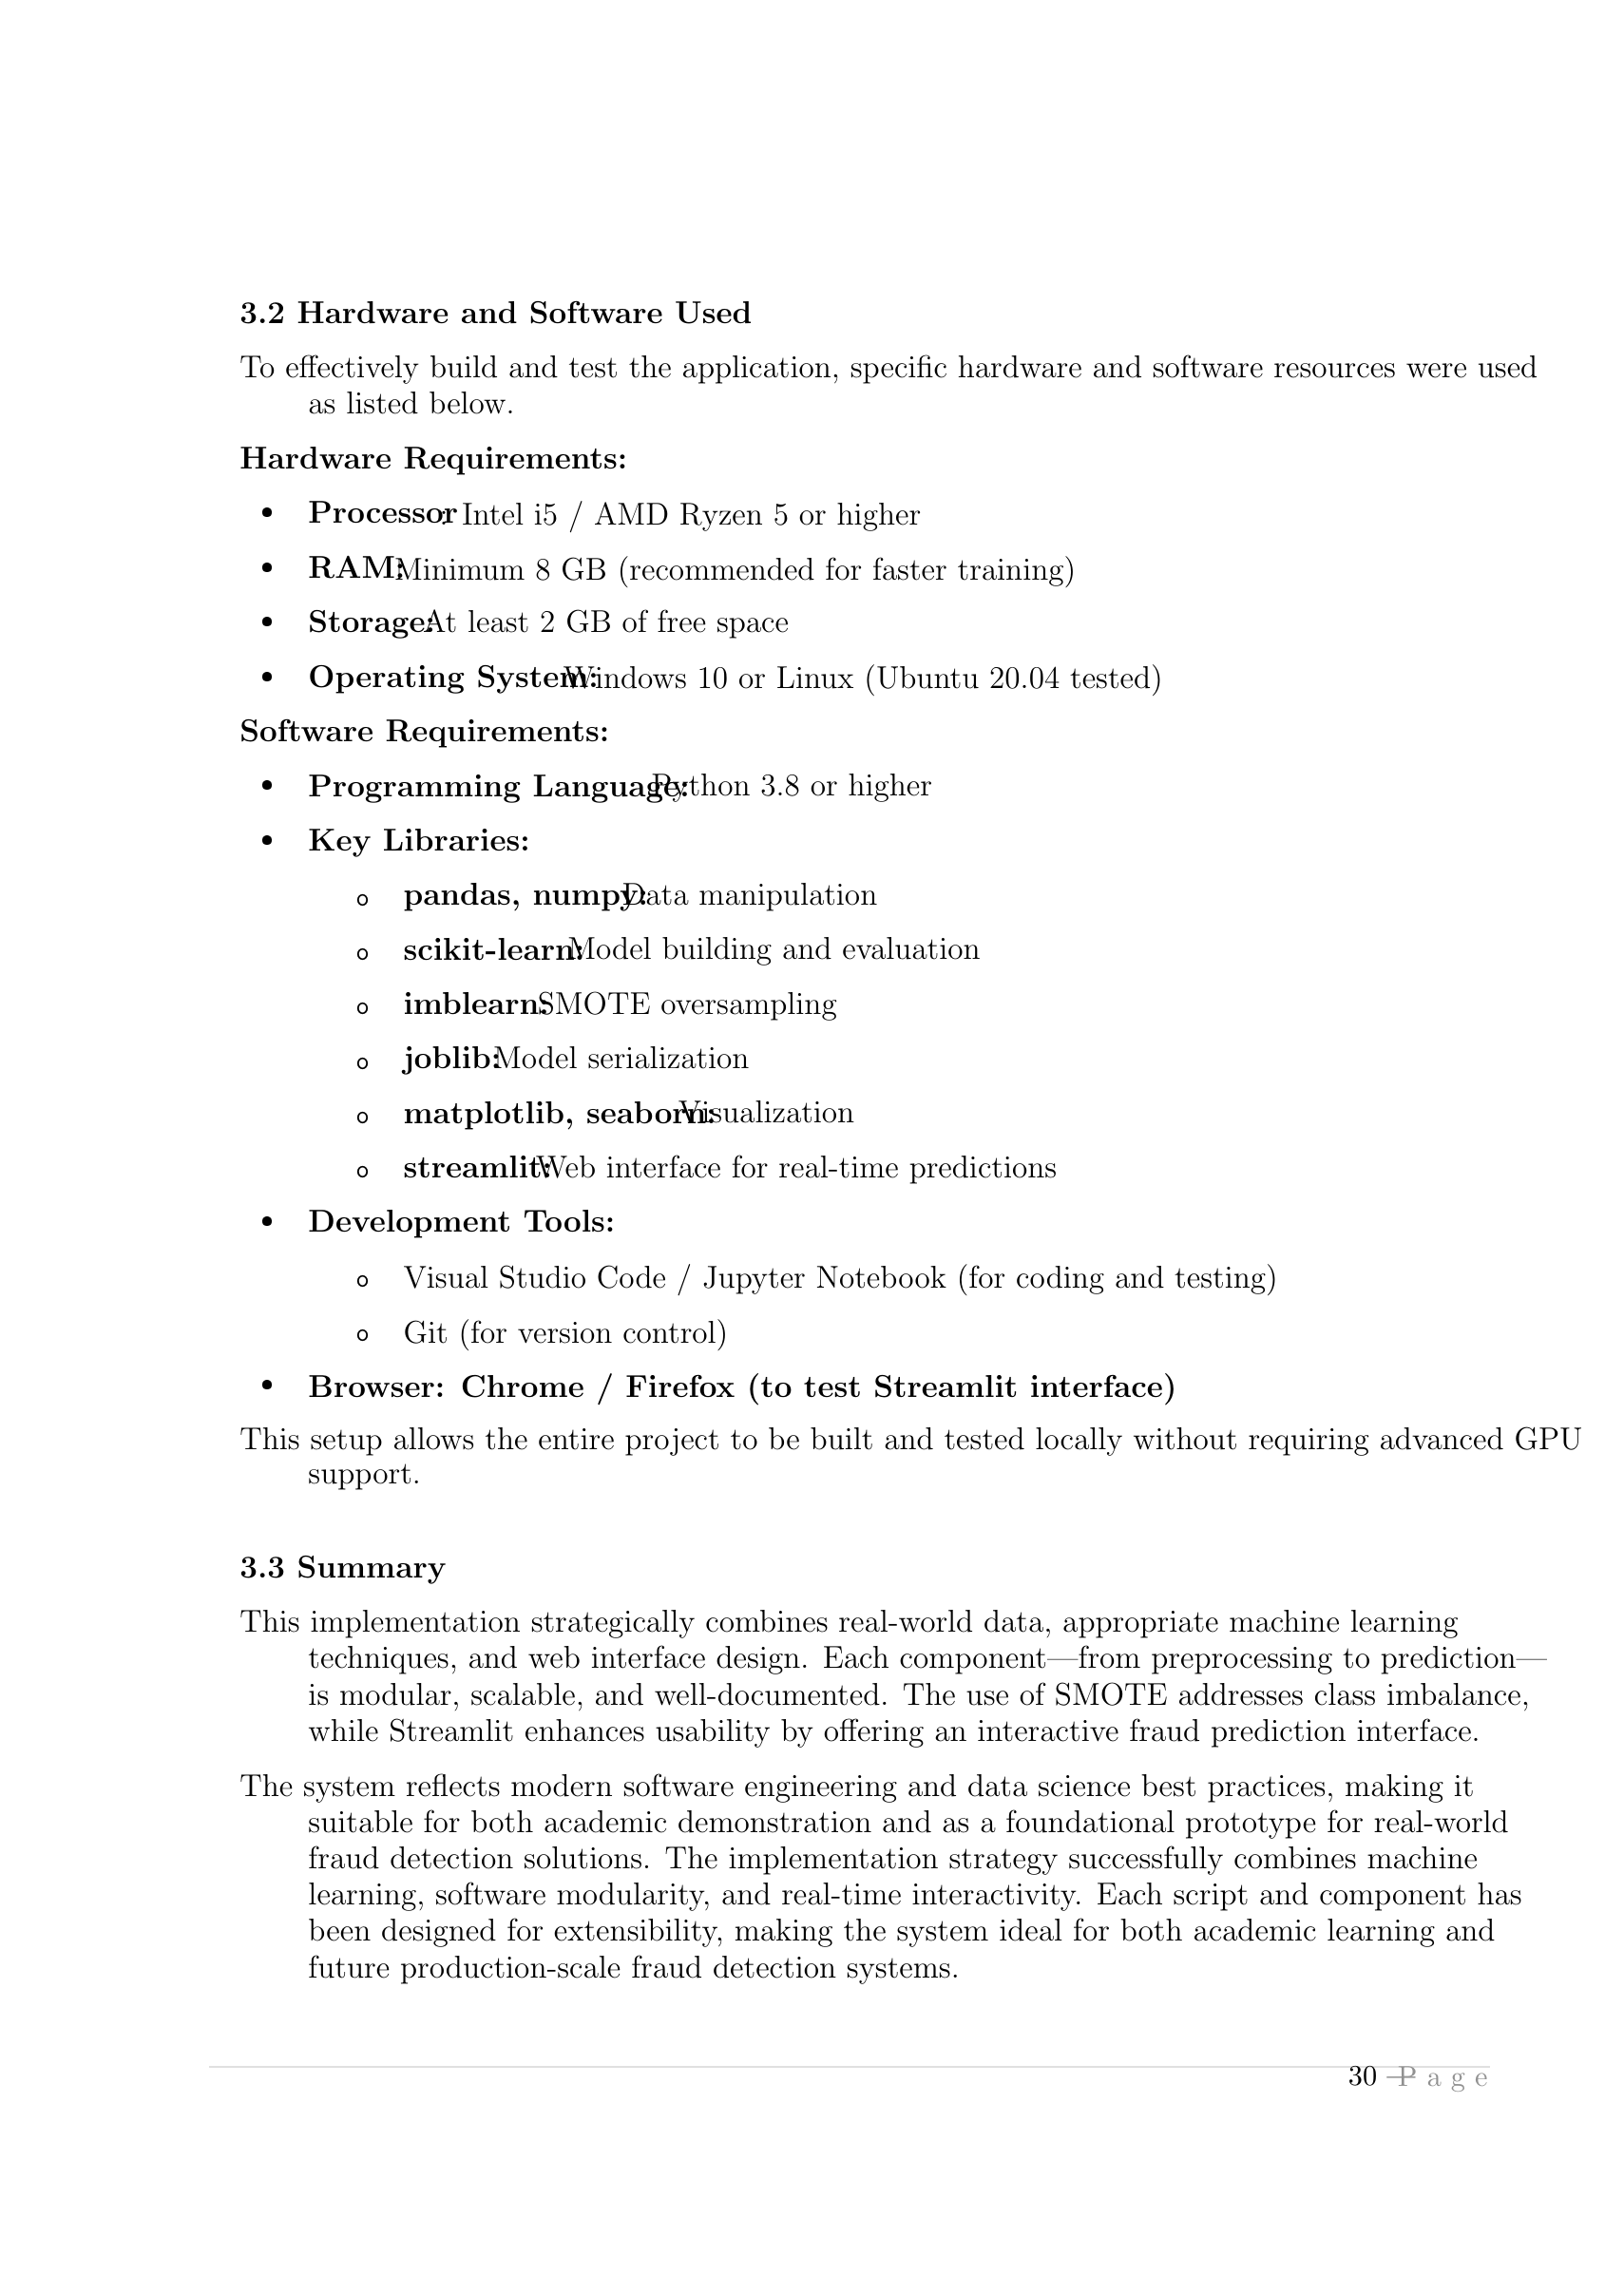
\begin{tikzpicture}[x=1bp,y=-1bp,inner sep=0pt,outer sep=0pt]
  \useasboundingbox (0,0) rectangle (595.20,841.92);
  \fill[fill=pdfcolor9] (69.38,772.78) rectangle (554.40,773.26);
  \node[anchor=north west,inner sep=0pt,outer sep=0pt] at (500.86,772.91) {{\fontsize{11.0bp}{13.2bp}\selectfont 30 | }};
  \node[anchor=north west,inner sep=0pt,outer sep=0pt] at (519.58,772.91) {{\fontsize{11.0bp}{13.2bp}\selectfont \textcolor{pdfcolor1}{P a g e}}};
  \node[anchor=north west,inner sep=0pt,outer sep=0pt] at (550.14,772.91) {{\fontsize{11.0bp}{13.2bp}\selectfont   }};
  \node[anchor=north west,inner sep=0pt,outer sep=0pt] at (80.90,104.37) {{\fontsize{12.0bp}{14.4bp}\selectfont \textbf{3.2 Hardware and Software Used }}};
  \node[anchor=north west,inner sep=0pt,outer sep=0pt] at (80.90,124.93) {{\fontsize{12.0bp}{14.4bp}\selectfont To effectively build and test the application, specific hardware and software resources were used }};
  \node[anchor=north west,inner sep=0pt,outer sep=0pt] at (106.85,138.61) {{\fontsize{12.0bp}{14.4bp}\selectfont as listed below. }};
  \node[anchor=north west,inner sep=0pt,outer sep=0pt] at (80.90,159.36) {{\fontsize{12.0bp}{14.4bp}\selectfont \textbf{Hardware Requirements: }}};
  \node[anchor=north west,inner sep=0pt,outer sep=0pt] at (88.85,182.40) {{\fontsize{10.1bp}{12.1bp}\selectfont •}};
  \node[anchor=north west,inner sep=0pt,outer sep=0pt] at (93.41,181.69) {\textsf{{\fontsize{10.1bp}{12.1bp}\selectfont  }}};
  \node[anchor=north west,inner sep=0pt,outer sep=0pt] at (106.85,180.00) {{\fontsize{12.0bp}{14.4bp}\selectfont \textbf{Processor}}};
  \node[anchor=north west,inner sep=0pt,outer sep=0pt] at (156.55,179.89) {{\fontsize{12.0bp}{14.4bp}\selectfont : Intel i5 / AMD Ryzen 5 or higher }};
  \node[anchor=north west,inner sep=0pt,outer sep=0pt] at (88.85,203.30) {{\fontsize{10.1bp}{12.1bp}\selectfont •}};
  \node[anchor=north west,inner sep=0pt,outer sep=0pt] at (93.41,202.59) {\textsf{{\fontsize{10.1bp}{12.1bp}\selectfont  }}};
  \node[anchor=north west,inner sep=0pt,outer sep=0pt] at (106.85,200.90) {{\fontsize{12.0bp}{14.4bp}\selectfont \textbf{RAM:}}};
  \node[anchor=north west,inner sep=0pt,outer sep=0pt] at (139.51,200.79) {{\fontsize{12.0bp}{14.4bp}\selectfont  Minimum 8 GB (recommended for faster training) }};
  \node[anchor=north west,inner sep=0pt,outer sep=0pt] at (88.85,223.94) {{\fontsize{10.1bp}{12.1bp}\selectfont •}};
  \node[anchor=north west,inner sep=0pt,outer sep=0pt] at (93.41,223.23) {\textsf{{\fontsize{10.1bp}{12.1bp}\selectfont  }}};
  \node[anchor=north west,inner sep=0pt,outer sep=0pt] at (106.85,221.54) {{\fontsize{12.0bp}{14.4bp}\selectfont \textbf{Storage:}}};
  \node[anchor=north west,inner sep=0pt,outer sep=0pt] at (150.31,221.43) {{\fontsize{12.0bp}{14.4bp}\selectfont  At least 2 GB of free space }};
  \node[anchor=north west,inner sep=0pt,outer sep=0pt] at (88.85,244.58) {{\fontsize{10.1bp}{12.1bp}\selectfont •}};
  \node[anchor=north west,inner sep=0pt,outer sep=0pt] at (93.41,243.87) {\textsf{{\fontsize{10.1bp}{12.1bp}\selectfont  }}};
  \node[anchor=north west,inner sep=0pt,outer sep=0pt] at (106.85,242.18) {{\fontsize{12.0bp}{14.4bp}\selectfont \textbf{Operating System:}}};
  \node[anchor=north west,inner sep=0pt,outer sep=0pt] at (203.38,242.07) {{\fontsize{12.0bp}{14.4bp}\selectfont  Windows 10 or Linux (Ubuntu 20.04 tested) }};
  \node[anchor=north west,inner sep=0pt,outer sep=0pt] at (80.90,262.82) {{\fontsize{12.0bp}{14.4bp}\selectfont \textbf{Software Requirements: }}};
  \node[anchor=north west,inner sep=0pt,outer sep=0pt] at (88.85,285.86) {{\fontsize{10.1bp}{12.1bp}\selectfont •}};
  \node[anchor=north west,inner sep=0pt,outer sep=0pt] at (93.41,285.15) {\textsf{{\fontsize{10.1bp}{12.1bp}\selectfont  }}};
  \node[anchor=north west,inner sep=0pt,outer sep=0pt] at (106.85,283.46) {{\fontsize{12.0bp}{14.4bp}\selectfont \textbf{Programming Language:}}};
  \node[anchor=north west,inner sep=0pt,outer sep=0pt] at (236.74,283.35) {{\fontsize{12.0bp}{14.4bp}\selectfont  Python 3.8 or higher }};
  \node[anchor=north west,inner sep=0pt,outer sep=0pt] at (88.85,306.53) {{\fontsize{10.1bp}{12.1bp}\selectfont •}};
  \node[anchor=north west,inner sep=0pt,outer sep=0pt] at (93.41,305.82) {\textsf{{\fontsize{10.1bp}{12.1bp}\selectfont  }}};
  \node[anchor=north west,inner sep=0pt,outer sep=0pt] at (106.85,304.13) {{\fontsize{12.0bp}{14.4bp}\selectfont \textbf{Key Libraries: }}};
  \node[anchor=north west,inner sep=0pt,outer sep=0pt] at (124.85,328.91) {\texttt{{\fontsize{10.1bp}{12.1bp}\selectfont o}}};
  \node[anchor=north west,inner sep=0pt,outer sep=0pt] at (130.85,326.46) {\textsf{{\fontsize{10.1bp}{12.1bp}\selectfont  }}};
  \node[anchor=north west,inner sep=0pt,outer sep=0pt] at (142.87,324.77) {{\fontsize{12.0bp}{14.4bp}\selectfont \textbf{pandas, numpy:}}};
  \node[anchor=north west,inner sep=0pt,outer sep=0pt] at (225.70,324.66) {{\fontsize{12.0bp}{14.4bp}\selectfont  Data manipulation }};
  \node[anchor=north west,inner sep=0pt,outer sep=0pt] at (124.85,349.55) {\texttt{{\fontsize{10.1bp}{12.1bp}\selectfont o}}};
  \node[anchor=north west,inner sep=0pt,outer sep=0pt] at (130.85,347.10) {\textsf{{\fontsize{10.1bp}{12.1bp}\selectfont  }}};
  \node[anchor=north west,inner sep=0pt,outer sep=0pt] at (142.87,345.41) {{\fontsize{12.0bp}{14.4bp}\selectfont \textbf{scikit-learn:}}};
  \node[anchor=north west,inner sep=0pt,outer sep=0pt] at (205.06,345.30) {{\fontsize{12.0bp}{14.4bp}\selectfont  Model building and evaluation }};
  \node[anchor=north west,inner sep=0pt,outer sep=0pt] at (124.85,370.19) {\texttt{{\fontsize{10.1bp}{12.1bp}\selectfont o}}};
  \node[anchor=north west,inner sep=0pt,outer sep=0pt] at (130.85,367.74) {\textsf{{\fontsize{10.1bp}{12.1bp}\selectfont  }}};
  \node[anchor=north west,inner sep=0pt,outer sep=0pt] at (142.87,366.05) {{\fontsize{12.0bp}{14.4bp}\selectfont \textbf{imblearn:}}};
  \node[anchor=north west,inner sep=0pt,outer sep=0pt] at (193.75,365.94) {{\fontsize{12.0bp}{14.4bp}\selectfont  SMOTE oversampling }};
  \node[anchor=north west,inner sep=0pt,outer sep=0pt] at (124.85,390.85) {\texttt{{\fontsize{10.1bp}{12.1bp}\selectfont o}}};
  \node[anchor=north west,inner sep=0pt,outer sep=0pt] at (130.85,388.40) {\textsf{{\fontsize{10.1bp}{12.1bp}\selectfont  }}};
  \node[anchor=north west,inner sep=0pt,outer sep=0pt] at (142.87,386.71) {{\fontsize{12.0bp}{14.4bp}\selectfont \textbf{joblib:}}};
  \node[anchor=north west,inner sep=0pt,outer sep=0pt] at (176.95,386.60) {{\fontsize{12.0bp}{14.4bp}\selectfont  Model serialization }};
  \node[anchor=north west,inner sep=0pt,outer sep=0pt] at (124.85,411.49) {\texttt{{\fontsize{10.1bp}{12.1bp}\selectfont o}}};
  \node[anchor=north west,inner sep=0pt,outer sep=0pt] at (130.85,409.04) {\textsf{{\fontsize{10.1bp}{12.1bp}\selectfont  }}};
  \node[anchor=north west,inner sep=0pt,outer sep=0pt] at (142.87,407.35) {{\fontsize{12.0bp}{14.4bp}\selectfont \textbf{matplotlib, seaborn:}}};
  \node[anchor=north west,inner sep=0pt,outer sep=0pt] at (247.06,407.24) {{\fontsize{12.0bp}{14.4bp}\selectfont  Visualization }};
  \node[anchor=north west,inner sep=0pt,outer sep=0pt] at (124.85,432.13) {\texttt{{\fontsize{10.1bp}{12.1bp}\selectfont o}}};
  \node[anchor=north west,inner sep=0pt,outer sep=0pt] at (130.85,429.68) {\textsf{{\fontsize{10.1bp}{12.1bp}\selectfont  }}};
  \node[anchor=north west,inner sep=0pt,outer sep=0pt] at (142.87,427.99) {{\fontsize{12.0bp}{14.4bp}\selectfont \textbf{streamlit:}}};
  \node[anchor=north west,inner sep=0pt,outer sep=0pt] at (193.03,427.88) {{\fontsize{12.0bp}{14.4bp}\selectfont  Web interface for real-time predictions }};
  \node[anchor=north west,inner sep=0pt,outer sep=0pt] at (88.85,451.03) {{\fontsize{10.1bp}{12.1bp}\selectfont •}};
  \node[anchor=north west,inner sep=0pt,outer sep=0pt] at (93.41,450.32) {\textsf{{\fontsize{10.1bp}{12.1bp}\selectfont  }}};
  \node[anchor=north west,inner sep=0pt,outer sep=0pt] at (106.85,448.63) {{\fontsize{12.0bp}{14.4bp}\selectfont \textbf{Development Tools: }}};
  \node[anchor=north west,inner sep=0pt,outer sep=0pt] at (124.85,473.43) {\texttt{{\fontsize{10.1bp}{12.1bp}\selectfont o}}};
  \node[anchor=north west,inner sep=0pt,outer sep=0pt] at (130.85,470.98) {\textsf{{\fontsize{10.1bp}{12.1bp}\selectfont  }}};
  \node[anchor=north west,inner sep=0pt,outer sep=0pt] at (142.87,469.18) {{\fontsize{12.0bp}{14.4bp}\selectfont Visual Studio Code / Jupyter Notebook (for coding and testing) }};
  \node[anchor=north west,inner sep=0pt,outer sep=0pt] at (124.85,494.07) {\texttt{{\fontsize{10.1bp}{12.1bp}\selectfont o}}};
  \node[anchor=north west,inner sep=0pt,outer sep=0pt] at (130.85,491.62) {\textsf{{\fontsize{10.1bp}{12.1bp}\selectfont  }}};
  \node[anchor=north west,inner sep=0pt,outer sep=0pt] at (142.87,489.82) {{\fontsize{12.0bp}{14.4bp}\selectfont Git (for version control) }};
  \node[anchor=north west,inner sep=0pt,outer sep=0pt] at (88.85,512.97) {{\fontsize{10.1bp}{12.1bp}\selectfont •}};
  \node[anchor=north west,inner sep=0pt,outer sep=0pt] at (93.41,512.26) {\textsf{{\fontsize{10.1bp}{12.1bp}\selectfont  }}};
  \node[anchor=north west,inner sep=0pt,outer sep=0pt] at (106.85,510.57) {{\fontsize{12.0bp}{14.4bp}\selectfont \textbf{Browser: Chrome / Firefox (to test Streamlit interface) }}};
  \node[anchor=north west,inner sep=0pt,outer sep=0pt] at (80.90,531.10) {{\fontsize{12.0bp}{14.4bp}\selectfont This setup allows the entire project to be built and tested locally without requiring advanced GPU }};
  \node[anchor=north west,inner sep=0pt,outer sep=0pt] at (106.85,544.81) {{\fontsize{12.0bp}{14.4bp}\selectfont support. }};
  \node[anchor=north west,inner sep=0pt,outer sep=0pt] at (80.90,579.48) {{\fontsize{12.0bp}{14.4bp}\selectfont \textbf{3.3 Summary }}};
  \node[anchor=north west,inner sep=0pt,outer sep=0pt] at (80.90,600.01) {{\fontsize{12.0bp}{14.4bp}\selectfont This implementation strategically combines real-world data, appropriate machine learning }};
  \node[anchor=north west,inner sep=0pt,outer sep=0pt] at (106.85,613.69) {{\fontsize{12.0bp}{14.4bp}\selectfont techniques, and web interface design. Each component---from preprocessing to prediction---}};
  \node[anchor=north west,inner sep=0pt,outer sep=0pt] at (106.85,627.61) {{\fontsize{12.0bp}{14.4bp}\selectfont is modular, scalable, and well-documented. The use of SMOTE addresses class imbalance, }};
  \node[anchor=north west,inner sep=0pt,outer sep=0pt] at (106.85,641.31) {{\fontsize{12.0bp}{14.4bp}\selectfont while Streamlit enhances usability by offering an interactive fraud prediction interface. }};
  \node[anchor=north west,inner sep=0pt,outer sep=0pt] at (80.90,662.19) {{\fontsize{12.0bp}{14.4bp}\selectfont The system reflects modern software engineering and data science best practices, making it }};
  \node[anchor=north west,inner sep=0pt,outer sep=0pt] at (106.85,675.87) {{\fontsize{12.0bp}{14.4bp}\selectfont suitable for both academic demonstration and as a foundational prototype for real-world }};
  \node[anchor=north west,inner sep=0pt,outer sep=0pt] at (106.85,689.55) {{\fontsize{12.0bp}{14.4bp}\selectfont fraud detection solutions. The implementation strategy successfully combines machine }};
  \node[anchor=north west,inner sep=0pt,outer sep=0pt] at (106.85,703.47) {{\fontsize{12.0bp}{14.4bp}\selectfont learning, software modularity, and real-time interactivity. Each script and component has }};
  \node[anchor=north west,inner sep=0pt,outer sep=0pt] at (106.85,717.18) {{\fontsize{12.0bp}{14.4bp}\selectfont been designed for extensibility, making the system ideal for both academic learning and }};
  \node[anchor=north west,inner sep=0pt,outer sep=0pt] at (106.85,731.10) {{\fontsize{12.0bp}{14.4bp}\selectfont future production-scale fraud detection systems. }};
\end{tikzpicture}
\newpage
\noindent

\begin{tikzpicture}[x=1bp,y=-1bp,inner sep=0pt,outer sep=0pt]
  \useasboundingbox (0,0) rectangle (595.20,841.92);
  \fill[fill=pdfcolor9] (69.38,772.78) rectangle (554.40,773.26);
  \fill[fill=black] (250.90,115.70) rectangle (328.23,117.14);
  \node[anchor=north west,inner sep=0pt,outer sep=0pt] at (500.86,772.91) {{\fontsize{11.0bp}{13.2bp}\selectfont 31 | }};
  \node[anchor=north west,inner sep=0pt,outer sep=0pt] at (519.58,772.91) {{\fontsize{11.0bp}{13.2bp}\selectfont \textcolor{pdfcolor1}{P a g e}}};
  \node[anchor=north west,inner sep=0pt,outer sep=0pt] at (550.14,772.91) {{\fontsize{11.0bp}{13.2bp}\selectfont   }};
  \node[anchor=north west,inner sep=0pt,outer sep=0pt] at (250.90,97.23) {{\fontsize{16.1bp}{19.3bp}\selectfont \textbf{4. DESIGN }}};
  \node[anchor=north west,inner sep=0pt,outer sep=0pt] at (70.82,128.77) {{\fontsize{12.0bp}{14.4bp}\selectfont This section outlines the architectural and structural design of the Credit Card Fraud Detection }};
  \node[anchor=north west,inner sep=0pt,outer sep=0pt] at (70.82,144.61) {{\fontsize{12.0bp}{14.4bp}\selectfont System. It includes the system flowchart to illustrate the operational logic and an Entity }};
  \node[anchor=north west,inner sep=0pt,outer sep=0pt] at (70.82,160.45) {{\fontsize{12.0bp}{14.4bp}\selectfont Relationship Diagram (ERD) to depict the data flow and interdependencies between major system }};
  \node[anchor=north west,inner sep=0pt,outer sep=0pt] at (70.82,176.29) {{\fontsize{12.0bp}{14.4bp}\selectfont components. }};
  \node[anchor=north west,inner sep=0pt,outer sep=0pt] at (70.82,228.26) {{\fontsize{12.0bp}{14.4bp}\selectfont \textbf{4.1 Flowchart }}};
  \node[anchor=north west,inner sep=0pt,outer sep=0pt] at (70.82,253.83) {{\fontsize{12.0bp}{14.4bp}\selectfont The flowchart represents the logical flow of the system from data loading to final prediction }};
  \node[anchor=north west,inner sep=0pt,outer sep=0pt] at (70.82,269.91) {{\fontsize{12.0bp}{14.4bp}\selectfont display. It provides a step-by-step structure of how the backend processes interact and how the user }};
  \node[anchor=north west,inner sep=0pt,outer sep=0pt] at (70.82,285.78) {{\fontsize{12.0bp}{14.4bp}\selectfont interfaces with the fraud detection model. }};
  \node[anchor=north west,inner sep=0pt,outer sep=0pt] at (70.82,311.46) {{\fontsize{12.0bp}{14.4bp}\selectfont Flow Steps: }};
  \node[anchor=north west,inner sep=0pt,outer sep=0pt] at (88.85,337.38) {{\fontsize{12.0bp}{14.4bp}\selectfont 1.}};
  \node[anchor=north west,inner sep=0pt,outer sep=0pt] at (97.97,337.12) {\textsf{{\fontsize{12.0bp}{14.4bp}\selectfont  }}};
  \node[anchor=north west,inner sep=0pt,outer sep=0pt] at (106.85,337.49) {{\fontsize{12.0bp}{14.4bp}\selectfont \textbf{Start:}}};
  \node[anchor=north west,inner sep=0pt,outer sep=0pt] at (136.85,337.38) {{\fontsize{12.0bp}{14.4bp}\selectfont  System is initialized. }};
  \node[anchor=north west,inner sep=0pt,outer sep=0pt] at (88.85,363.30) {{\fontsize{12.0bp}{14.4bp}\selectfont 2.}};
  \node[anchor=north west,inner sep=0pt,outer sep=0pt] at (97.97,363.04) {\textsf{{\fontsize{12.0bp}{14.4bp}\selectfont  }}};
  \node[anchor=north west,inner sep=0pt,outer sep=0pt] at (106.85,363.41) {{\fontsize{12.0bp}{14.4bp}\selectfont \textbf{Load Dataset:}}};
  \node[anchor=north west,inner sep=0pt,outer sep=0pt] at (179.35,363.30) {{\fontsize{12.0bp}{14.4bp}\selectfont  The creditcard.csv file is loaded using pandas. }};
  \node[anchor=north west,inner sep=0pt,outer sep=0pt] at (88.85,389.35) {{\fontsize{12.0bp}{14.4bp}\selectfont \textbf{3.}}};
  \node[anchor=north west,inner sep=0pt,outer sep=0pt] at (97.97,389.04) {\textsf{{\fontsize{12.0bp}{14.4bp}\selectfont \textbf{ }}}};
  \node[anchor=north west,inner sep=0pt,outer sep=0pt] at (106.85,389.35) {{\fontsize{12.0bp}{14.4bp}\selectfont \textbf{Data Preprocessing: }}};
  \node[anchor=north west,inner sep=0pt,outer sep=0pt] at (124.85,419.41) {\texttt{{\fontsize{10.1bp}{12.1bp}\selectfont o}}};
  \node[anchor=north west,inner sep=0pt,outer sep=0pt] at (130.85,416.96) {\textsf{{\fontsize{10.1bp}{12.1bp}\selectfont  }}};
  \node[anchor=north west,inner sep=0pt,outer sep=0pt] at (142.87,415.16) {{\fontsize{12.0bp}{14.4bp}\selectfont Scale the Time and Amount fields using StandardScaler. }};
  \node[anchor=north west,inner sep=0pt,outer sep=0pt] at (124.85,445.09) {\texttt{{\fontsize{10.1bp}{12.1bp}\selectfont o}}};
  \node[anchor=north west,inner sep=0pt,outer sep=0pt] at (130.85,442.64) {\textsf{{\fontsize{10.1bp}{12.1bp}\selectfont  }}};
  \node[anchor=north west,inner sep=0pt,outer sep=0pt] at (142.87,440.84) {{\fontsize{12.0bp}{14.4bp}\selectfont Apply SMOTE to synthetically balance the dataset. }};
  \node[anchor=north west,inner sep=0pt,outer sep=0pt] at (88.85,466.89) {{\fontsize{12.0bp}{14.4bp}\selectfont \textbf{4.}}};
  \node[anchor=north west,inner sep=0pt,outer sep=0pt] at (97.97,466.58) {\textsf{{\fontsize{12.0bp}{14.4bp}\selectfont \textbf{ }}}};
  \node[anchor=north west,inner sep=0pt,outer sep=0pt] at (106.85,466.89) {{\fontsize{12.0bp}{14.4bp}\selectfont \textbf{Model Training: }}};
  \node[anchor=north west,inner sep=0pt,outer sep=0pt] at (124.85,496.95) {\texttt{{\fontsize{10.1bp}{12.1bp}\selectfont o}}};
  \node[anchor=north west,inner sep=0pt,outer sep=0pt] at (130.85,494.50) {\textsf{{\fontsize{10.1bp}{12.1bp}\selectfont  }}};
  \node[anchor=north west,inner sep=0pt,outer sep=0pt] at (142.87,492.70) {{\fontsize{12.0bp}{14.4bp}\selectfont The RandomForestClassifier is trained on the preprocessed and resampled dataset. }};
  \node[anchor=north west,inner sep=0pt,outer sep=0pt] at (88.85,518.73) {{\fontsize{12.0bp}{14.4bp}\selectfont \textbf{5.}}};
  \node[anchor=north west,inner sep=0pt,outer sep=0pt] at (97.97,518.42) {\textsf{{\fontsize{12.0bp}{14.4bp}\selectfont \textbf{ }}}};
  \node[anchor=north west,inner sep=0pt,outer sep=0pt] at (106.85,518.73) {{\fontsize{12.0bp}{14.4bp}\selectfont \textbf{Evaluation: }}};
  \node[anchor=north west,inner sep=0pt,outer sep=0pt] at (124.85,548.82) {\texttt{{\fontsize{10.1bp}{12.1bp}\selectfont o}}};
  \node[anchor=north west,inner sep=0pt,outer sep=0pt] at (130.85,546.37) {\textsf{{\fontsize{10.1bp}{12.1bp}\selectfont  }}};
  \node[anchor=north west,inner sep=0pt,outer sep=0pt] at (142.87,544.57) {{\fontsize{12.0bp}{14.4bp}\selectfont The model is evaluated using classification metrics (Accuracy, Precision, Recall, F1-}};
  \node[anchor=north west,inner sep=0pt,outer sep=0pt] at (142.87,560.41) {{\fontsize{12.0bp}{14.4bp}\selectfont Score, ROC-AUC). }};
  \node[anchor=north west,inner sep=0pt,outer sep=0pt] at (124.85,590.34) {\texttt{{\fontsize{10.1bp}{12.1bp}\selectfont o}}};
  \node[anchor=north west,inner sep=0pt,outer sep=0pt] at (130.85,587.89) {\textsf{{\fontsize{10.1bp}{12.1bp}\selectfont  }}};
  \node[anchor=north west,inner sep=0pt,outer sep=0pt] at (142.87,586.09) {{\fontsize{12.0bp}{14.4bp}\selectfont Confusion matrix and ROC curve are generated. }};
  \node[anchor=north west,inner sep=0pt,outer sep=0pt] at (88.85,612.12) {{\fontsize{12.0bp}{14.4bp}\selectfont \textbf{6.}}};
  \node[anchor=north west,inner sep=0pt,outer sep=0pt] at (97.97,611.81) {\textsf{{\fontsize{12.0bp}{14.4bp}\selectfont \textbf{ }}}};
  \node[anchor=north west,inner sep=0pt,outer sep=0pt] at (106.85,612.12) {{\fontsize{12.0bp}{14.4bp}\selectfont \textbf{Model Saving: }}};
  \node[anchor=north west,inner sep=0pt,outer sep=0pt] at (124.85,642.20) {\texttt{{\fontsize{10.1bp}{12.1bp}\selectfont o}}};
  \node[anchor=north west,inner sep=0pt,outer sep=0pt] at (130.85,639.75) {\textsf{{\fontsize{10.1bp}{12.1bp}\selectfont  }}};
  \node[anchor=north west,inner sep=0pt,outer sep=0pt] at (142.87,637.95) {{\fontsize{12.0bp}{14.4bp}\selectfont The trained model is saved using joblib. }};
  \node[anchor=north west,inner sep=0pt,outer sep=0pt] at (88.85,663.98) {{\fontsize{12.0bp}{14.4bp}\selectfont \textbf{7.}}};
  \node[anchor=north west,inner sep=0pt,outer sep=0pt] at (97.97,663.67) {\textsf{{\fontsize{12.0bp}{14.4bp}\selectfont \textbf{ }}}};
  \node[anchor=north west,inner sep=0pt,outer sep=0pt] at (106.85,663.98) {{\fontsize{12.0bp}{14.4bp}\selectfont \textbf{UI Interaction: }}};
  \node[anchor=north west,inner sep=0pt,outer sep=0pt] at (124.85,694.04) {\texttt{{\fontsize{10.1bp}{12.1bp}\selectfont o}}};
  \node[anchor=north west,inner sep=0pt,outer sep=0pt] at (130.85,691.59) {\textsf{{\fontsize{10.1bp}{12.1bp}\selectfont  }}};
  \node[anchor=north west,inner sep=0pt,outer sep=0pt] at (142.87,689.79) {{\fontsize{12.0bp}{14.4bp}\selectfont The Streamlit interface is launched. }};
  \node[anchor=north west,inner sep=0pt,outer sep=0pt] at (124.85,719.75) {\texttt{{\fontsize{10.1bp}{12.1bp}\selectfont o}}};
  \node[anchor=north west,inner sep=0pt,outer sep=0pt] at (130.85,717.30) {\textsf{{\fontsize{10.1bp}{12.1bp}\selectfont  }}};
  \node[anchor=north west,inner sep=0pt,outer sep=0pt] at (142.87,715.50) {{\fontsize{12.0bp}{14.4bp}\selectfont User inputs transaction details (features V1--V28, Amount). }};
  \node[anchor=north west,inner sep=0pt,outer sep=0pt] at (88.85,741.53) {{\fontsize{12.0bp}{14.4bp}\selectfont \textbf{8.}}};
  \node[anchor=north west,inner sep=0pt,outer sep=0pt] at (97.97,741.22) {\textsf{{\fontsize{12.0bp}{14.4bp}\selectfont \textbf{ }}}};
  \node[anchor=north west,inner sep=0pt,outer sep=0pt] at (106.85,741.53) {{\fontsize{12.0bp}{14.4bp}\selectfont \textbf{Prediction: }}};
\end{tikzpicture}
\newpage
\noindent
\begin{tikzpicture}[x=1bp,y=-1bp,inner sep=0pt,outer sep=0pt]
  \useasboundingbox (0,0) rectangle (595.20,841.92);
  \fill[fill=pdfcolor9] (69.38,772.78) rectangle (554.40,773.26);
  \node[anchor=north west,inner sep=0pt] at (106.90,188.53) {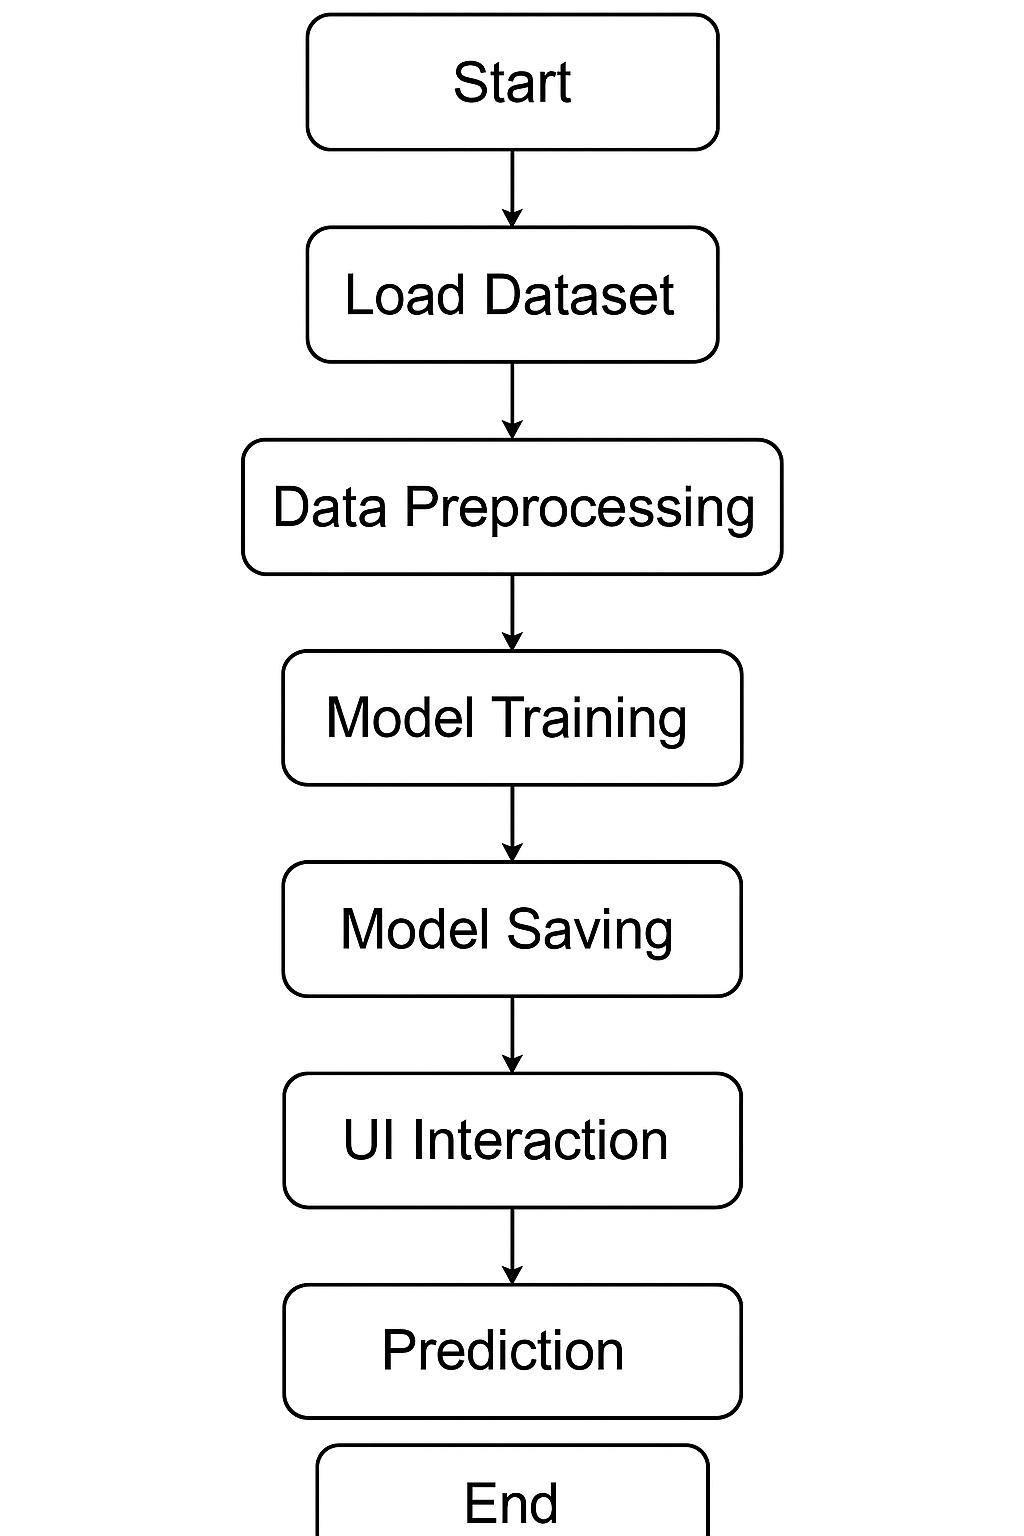
\includegraphics[width=309.45bp,height=463.97bp]{images/image_p40_37.png}};
  \node[anchor=north west,inner sep=0pt,outer sep=0pt] at (500.86,772.91) {{\fontsize{11.0bp}{13.2bp}\selectfont 32 | }};
  \node[anchor=north west,inner sep=0pt,outer sep=0pt] at (519.58,772.91) {{\fontsize{11.0bp}{13.2bp}\selectfont \textcolor{pdfcolor1}{P a g e}}};
  \node[anchor=north west,inner sep=0pt,outer sep=0pt] at (550.14,772.91) {{\fontsize{11.0bp}{13.2bp}\selectfont   }};
  \node[anchor=north west,inner sep=0pt,outer sep=0pt] at (124.85,87.87) {\texttt{{\fontsize{10.1bp}{12.1bp}\selectfont o}}};
  \node[anchor=north west,inner sep=0pt,outer sep=0pt] at (130.85,85.42) {\textsf{{\fontsize{10.1bp}{12.1bp}\selectfont  }}};
  \node[anchor=north west,inner sep=0pt,outer sep=0pt] at (142.87,83.62) {{\fontsize{12.0bp}{14.4bp}\selectfont The model predicts whether the transaction is fraudulent or legitimate. }};
  \node[anchor=north west,inner sep=0pt,outer sep=0pt] at (124.85,113.79) {\texttt{{\fontsize{10.1bp}{12.1bp}\selectfont o}}};
  \node[anchor=north west,inner sep=0pt,outer sep=0pt] at (130.85,111.34) {\textsf{{\fontsize{10.1bp}{12.1bp}\selectfont  }}};
  \node[anchor=north west,inner sep=0pt,outer sep=0pt] at (142.87,109.54) {{\fontsize{12.0bp}{14.4bp}\selectfont The result and confidence score are displayed. }};
  \node[anchor=north west,inner sep=0pt,outer sep=0pt] at (88.85,135.49) {{\fontsize{12.0bp}{14.4bp}\selectfont 9.}};
  \node[anchor=north west,inner sep=0pt,outer sep=0pt] at (97.97,135.23) {\textsf{{\fontsize{12.0bp}{14.4bp}\selectfont  }}};
  \node[anchor=north west,inner sep=0pt,outer sep=0pt] at (106.85,135.60) {{\fontsize{12.0bp}{14.4bp}\selectfont \textbf{End:}}};
  \node[anchor=north west,inner sep=0pt,outer sep=0pt] at (132.29,135.49) {{\fontsize{12.0bp}{14.4bp}\selectfont  The system awaits further inputs or closes. }};
  \node[anchor=north west,inner sep=0pt,outer sep=0pt] at (88.85,161.52) {{\fontsize{12.0bp}{14.4bp}\selectfont \textbf{Flowchart:}}};
  \node[anchor=north west,inner sep=0pt,outer sep=0pt] at (145.51,161.41) {{\fontsize{12.0bp}{14.4bp}\selectfont  }};
  \node[anchor=north west,inner sep=0pt,outer sep=0pt] at (70.82,663.39) {{\fontsize{12.0bp}{14.4bp}\selectfont This flow ensures that each component is tightly integrated but independently testable, maintaining }};
  \node[anchor=north west,inner sep=0pt,outer sep=0pt] at (70.82,679.23) {{\fontsize{12.0bp}{14.4bp}\selectfont robustness and flexibility. }};
  \node[anchor=north west,inner sep=0pt,outer sep=0pt] at (70.82,731.21) {{\fontsize{12.0bp}{14.4bp}\selectfont \textbf{7.2 Entity Relationship Diagram (ERD) }}};
\end{tikzpicture}
\newpage
\noindent
\begin{tikzpicture}[x=1bp,y=-1bp,inner sep=0pt,outer sep=0pt]
  \useasboundingbox (0,0) rectangle (595.20,841.92);
  \fill[fill=pdfcolor9] (69.38,772.78) rectangle (554.40,773.26);
  \node[anchor=north west,inner sep=0pt,outer sep=0pt] at (500.86,772.91) {{\fontsize{11.0bp}{13.2bp}\selectfont 33 | }};
  \node[anchor=north west,inner sep=0pt,outer sep=0pt] at (519.58,772.91) {{\fontsize{11.0bp}{13.2bp}\selectfont \textcolor{pdfcolor1}{P a g e}}};
  \node[anchor=north west,inner sep=0pt,outer sep=0pt] at (550.14,772.91) {{\fontsize{11.0bp}{13.2bp}\selectfont   }};
  \node[anchor=north west,inner sep=0pt,outer sep=0pt] at (70.82,83.62) {{\fontsize{12.0bp}{14.4bp}\selectfont The ERD defines how different entities within the system relate to each other, particularly in terms }};
  \node[anchor=north west,inner sep=0pt,outer sep=0pt] at (70.82,99.46) {{\fontsize{12.0bp}{14.4bp}\selectfont of data attributes and model interactions. Each entity represents a logical component or process }};
  \node[anchor=north west,inner sep=0pt,outer sep=0pt] at (70.82,115.57) {{\fontsize{12.0bp}{14.4bp}\selectfont within the fraud detection system. }};
  \node[anchor=north west,inner sep=0pt,outer sep=0pt] at (70.82,141.25) {{\fontsize{12.0bp}{14.4bp}\selectfont Entities and Attributes: }};
  \node[anchor=north west,inner sep=0pt,outer sep=0pt] at (88.85,167.28) {{\fontsize{12.0bp}{14.4bp}\selectfont \textbf{1.}}};
  \node[anchor=north west,inner sep=0pt,outer sep=0pt] at (97.97,166.97) {\textsf{{\fontsize{12.0bp}{14.4bp}\selectfont \textbf{ }}}};
  \node[anchor=north west,inner sep=0pt,outer sep=0pt] at (106.85,167.28) {{\fontsize{12.0bp}{14.4bp}\selectfont \textbf{Transaction: }}};
  \node[anchor=north west,inner sep=0pt,outer sep=0pt] at (124.85,197.34) {\texttt{{\fontsize{10.1bp}{12.1bp}\selectfont o}}};
  \node[anchor=north west,inner sep=0pt,outer sep=0pt] at (130.85,194.89) {\textsf{{\fontsize{10.1bp}{12.1bp}\selectfont  }}};
  \node[anchor=north west,inner sep=0pt,outer sep=0pt] at (142.87,193.09) {{\fontsize{12.0bp}{14.4bp}\selectfont Transaction\_ID (PK) }};
  \node[anchor=north west,inner sep=0pt,outer sep=0pt] at (124.85,223.28) {\texttt{{\fontsize{10.1bp}{12.1bp}\selectfont o}}};
  \node[anchor=north west,inner sep=0pt,outer sep=0pt] at (130.85,220.83) {\textsf{{\fontsize{10.1bp}{12.1bp}\selectfont  }}};
  \node[anchor=north west,inner sep=0pt,outer sep=0pt] at (142.87,219.03) {{\fontsize{12.0bp}{14.4bp}\selectfont Time }};
  \node[anchor=north west,inner sep=0pt,outer sep=0pt] at (124.85,249.20) {\texttt{{\fontsize{10.1bp}{12.1bp}\selectfont o}}};
  \node[anchor=north west,inner sep=0pt,outer sep=0pt] at (130.85,246.75) {\textsf{{\fontsize{10.1bp}{12.1bp}\selectfont  }}};
  \node[anchor=north west,inner sep=0pt,outer sep=0pt] at (142.87,244.95) {{\fontsize{12.0bp}{14.4bp}\selectfont Amount }};
  \node[anchor=north west,inner sep=0pt,outer sep=0pt] at (124.85,274.88) {\texttt{{\fontsize{10.1bp}{12.1bp}\selectfont o}}};
  \node[anchor=north west,inner sep=0pt,outer sep=0pt] at (130.85,272.43) {\textsf{{\fontsize{10.1bp}{12.1bp}\selectfont  }}};
  \node[anchor=north west,inner sep=0pt,outer sep=0pt] at (142.87,270.63) {{\fontsize{12.0bp}{14.4bp}\selectfont Class (0 = Legitimate, 1 = Fraudulent) }};
  \node[anchor=north west,inner sep=0pt,outer sep=0pt] at (88.85,296.69) {{\fontsize{12.0bp}{14.4bp}\selectfont \textbf{2.}}};
  \node[anchor=north west,inner sep=0pt,outer sep=0pt] at (97.97,296.38) {\textsf{{\fontsize{12.0bp}{14.4bp}\selectfont \textbf{ }}}};
  \node[anchor=north west,inner sep=0pt,outer sep=0pt] at (106.85,296.69) {{\fontsize{12.0bp}{14.4bp}\selectfont \textbf{Feature: }}};
  \node[anchor=north west,inner sep=0pt,outer sep=0pt] at (124.85,326.75) {\texttt{{\fontsize{10.1bp}{12.1bp}\selectfont o}}};
  \node[anchor=north west,inner sep=0pt,outer sep=0pt] at (130.85,324.30) {\textsf{{\fontsize{10.1bp}{12.1bp}\selectfont  }}};
  \node[anchor=north west,inner sep=0pt,outer sep=0pt] at (142.87,322.50) {{\fontsize{12.0bp}{14.4bp}\selectfont Feature\_ID (PK) }};
  \node[anchor=north west,inner sep=0pt,outer sep=0pt] at (124.85,352.67) {\texttt{{\fontsize{10.1bp}{12.1bp}\selectfont o}}};
  \node[anchor=north west,inner sep=0pt,outer sep=0pt] at (130.85,350.22) {\textsf{{\fontsize{10.1bp}{12.1bp}\selectfont  }}};
  \node[anchor=north west,inner sep=0pt,outer sep=0pt] at (142.87,348.42) {{\fontsize{12.0bp}{14.4bp}\selectfont Transaction\_ID (FK) }};
  \node[anchor=north west,inner sep=0pt,outer sep=0pt] at (124.85,378.37) {\texttt{{\fontsize{10.1bp}{12.1bp}\selectfont o}}};
  \node[anchor=north west,inner sep=0pt,outer sep=0pt] at (130.85,375.92) {\textsf{{\fontsize{10.1bp}{12.1bp}\selectfont  }}};
  \node[anchor=north west,inner sep=0pt,outer sep=0pt] at (142.87,374.12) {{\fontsize{12.0bp}{14.4bp}\selectfont V1 to V28 (anonymized PCA components) }};
  \node[anchor=north west,inner sep=0pt,outer sep=0pt] at (88.85,400.15) {{\fontsize{12.0bp}{14.4bp}\selectfont \textbf{3.}}};
  \node[anchor=north west,inner sep=0pt,outer sep=0pt] at (97.97,399.84) {\textsf{{\fontsize{12.0bp}{14.4bp}\selectfont \textbf{ }}}};
  \node[anchor=north west,inner sep=0pt,outer sep=0pt] at (106.85,400.15) {{\fontsize{12.0bp}{14.4bp}\selectfont \textbf{Preprocessing: }}};
  \node[anchor=north west,inner sep=0pt,outer sep=0pt] at (124.85,430.21) {\texttt{{\fontsize{10.1bp}{12.1bp}\selectfont o}}};
  \node[anchor=north west,inner sep=0pt,outer sep=0pt] at (130.85,427.76) {\textsf{{\fontsize{10.1bp}{12.1bp}\selectfont  }}};
  \node[anchor=north west,inner sep=0pt,outer sep=0pt] at (142.87,425.96) {{\fontsize{12.0bp}{14.4bp}\selectfont Preprocess\_ID (PK) }};
  \node[anchor=north west,inner sep=0pt,outer sep=0pt] at (124.85,456.13) {\texttt{{\fontsize{10.1bp}{12.1bp}\selectfont o}}};
  \node[anchor=north west,inner sep=0pt,outer sep=0pt] at (130.85,453.68) {\textsf{{\fontsize{10.1bp}{12.1bp}\selectfont  }}};
  \node[anchor=north west,inner sep=0pt,outer sep=0pt] at (142.87,451.88) {{\fontsize{12.0bp}{14.4bp}\selectfont Transaction\_ID (FK) }};
  \node[anchor=north west,inner sep=0pt,outer sep=0pt] at (124.85,482.07) {\texttt{{\fontsize{10.1bp}{12.1bp}\selectfont o}}};
  \node[anchor=north west,inner sep=0pt,outer sep=0pt] at (130.85,479.62) {\textsf{{\fontsize{10.1bp}{12.1bp}\selectfont  }}};
  \node[anchor=north west,inner sep=0pt,outer sep=0pt] at (142.87,477.82) {{\fontsize{12.0bp}{14.4bp}\selectfont Scaling\_Method (e.g., StandardScaler) }};
  \node[anchor=north west,inner sep=0pt,outer sep=0pt] at (124.85,507.75) {\texttt{{\fontsize{10.1bp}{12.1bp}\selectfont o}}};
  \node[anchor=north west,inner sep=0pt,outer sep=0pt] at (130.85,505.30) {\textsf{{\fontsize{10.1bp}{12.1bp}\selectfont  }}};
  \node[anchor=north west,inner sep=0pt,outer sep=0pt] at (142.87,503.50) {{\fontsize{12.0bp}{14.4bp}\selectfont Imbalance\_Technique (e.g., SMOTE) }};
  \node[anchor=north west,inner sep=0pt,outer sep=0pt] at (88.85,529.53) {{\fontsize{12.0bp}{14.4bp}\selectfont \textbf{4.}}};
  \node[anchor=north west,inner sep=0pt,outer sep=0pt] at (97.97,529.22) {\textsf{{\fontsize{12.0bp}{14.4bp}\selectfont \textbf{ }}}};
  \node[anchor=north west,inner sep=0pt,outer sep=0pt] at (106.85,529.53) {{\fontsize{12.0bp}{14.4bp}\selectfont \textbf{Model: }}};
  \node[anchor=north west,inner sep=0pt,outer sep=0pt] at (124.85,559.62) {\texttt{{\fontsize{10.1bp}{12.1bp}\selectfont o}}};
  \node[anchor=north west,inner sep=0pt,outer sep=0pt] at (130.85,557.17) {\textsf{{\fontsize{10.1bp}{12.1bp}\selectfont  }}};
  \node[anchor=north west,inner sep=0pt,outer sep=0pt] at (142.87,555.37) {{\fontsize{12.0bp}{14.4bp}\selectfont Model\_ID (PK) }};
  \node[anchor=north west,inner sep=0pt,outer sep=0pt] at (124.85,585.54) {\texttt{{\fontsize{10.1bp}{12.1bp}\selectfont o}}};
  \node[anchor=north west,inner sep=0pt,outer sep=0pt] at (130.85,583.09) {\textsf{{\fontsize{10.1bp}{12.1bp}\selectfont  }}};
  \node[anchor=north west,inner sep=0pt,outer sep=0pt] at (142.87,581.29) {{\fontsize{12.0bp}{14.4bp}\selectfont Model\_Name (e.g., RandomForest) }};
  \node[anchor=north west,inner sep=0pt,outer sep=0pt] at (124.85,611.46) {\texttt{{\fontsize{10.1bp}{12.1bp}\selectfont o}}};
  \node[anchor=north west,inner sep=0pt,outer sep=0pt] at (130.85,609.01) {\textsf{{\fontsize{10.1bp}{12.1bp}\selectfont  }}};
  \node[anchor=north west,inner sep=0pt,outer sep=0pt] at (142.87,607.21) {{\fontsize{12.0bp}{14.4bp}\selectfont Accuracy }};
  \node[anchor=north west,inner sep=0pt,outer sep=0pt] at (124.85,637.16) {\texttt{{\fontsize{10.1bp}{12.1bp}\selectfont o}}};
  \node[anchor=north west,inner sep=0pt,outer sep=0pt] at (130.85,634.71) {\textsf{{\fontsize{10.1bp}{12.1bp}\selectfont  }}};
  \node[anchor=north west,inner sep=0pt,outer sep=0pt] at (142.87,632.91) {{\fontsize{12.0bp}{14.4bp}\selectfont F1\_Score }};
  \node[anchor=north west,inner sep=0pt,outer sep=0pt] at (124.85,663.08) {\texttt{{\fontsize{10.1bp}{12.1bp}\selectfont o}}};
  \node[anchor=north west,inner sep=0pt,outer sep=0pt] at (130.85,660.63) {\textsf{{\fontsize{10.1bp}{12.1bp}\selectfont  }}};
  \node[anchor=north west,inner sep=0pt,outer sep=0pt] at (142.87,658.83) {{\fontsize{12.0bp}{14.4bp}\selectfont ROC\_AUC\_Score }};
  \node[anchor=north west,inner sep=0pt,outer sep=0pt] at (88.85,684.75) {{\fontsize{12.0bp}{14.4bp}\selectfont 5.}};
  \node[anchor=north west,inner sep=0pt,outer sep=0pt] at (97.97,684.49) {\textsf{{\fontsize{12.0bp}{14.4bp}\selectfont  }}};
  \node[anchor=north west,inner sep=0pt,outer sep=0pt] at (106.85,684.75) {{\fontsize{12.0bp}{14.4bp}\selectfont Prediction: }};
  \node[anchor=north west,inner sep=0pt,outer sep=0pt] at (124.85,714.92) {\texttt{{\fontsize{10.1bp}{12.1bp}\selectfont o}}};
  \node[anchor=north west,inner sep=0pt,outer sep=0pt] at (130.85,712.47) {\textsf{{\fontsize{10.1bp}{12.1bp}\selectfont  }}};
  \node[anchor=north west,inner sep=0pt,outer sep=0pt] at (142.87,710.67) {{\fontsize{12.0bp}{14.4bp}\selectfont Prediction\_ID (PK) }};
  \node[anchor=north west,inner sep=0pt,outer sep=0pt] at (124.85,740.62) {\texttt{{\fontsize{10.1bp}{12.1bp}\selectfont o}}};
  \node[anchor=north west,inner sep=0pt,outer sep=0pt] at (130.85,738.18) {\textsf{{\fontsize{10.1bp}{12.1bp}\selectfont  }}};
  \node[anchor=north west,inner sep=0pt,outer sep=0pt] at (142.87,736.38) {{\fontsize{12.0bp}{14.4bp}\selectfont Transaction\_ID (FK) }};
\end{tikzpicture}
\newpage
\noindent
\begin{tikzpicture}[x=1bp,y=-1bp,inner sep=0pt,outer sep=0pt]
  \useasboundingbox (0,0) rectangle (595.20,841.92);
  \fill[fill=pdfcolor9] (69.38,772.78) rectangle (554.40,773.26);
  \node[anchor=north west,inner sep=0pt] at (70.90,317.87) {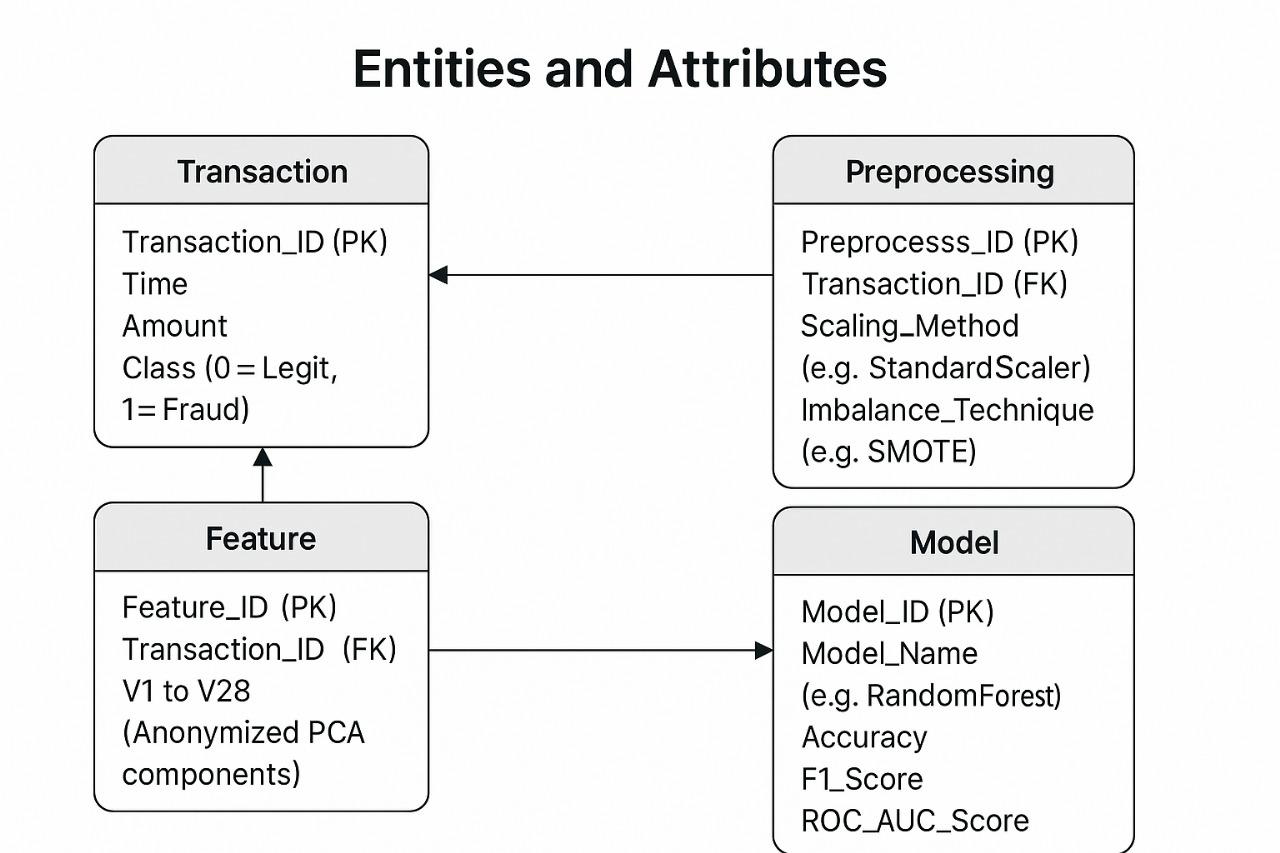
\includegraphics[width=481.95bp,height=321.20bp]{images/image_p42_38.png}};
  \node[anchor=north west,inner sep=0pt,outer sep=0pt] at (500.86,772.91) {{\fontsize{11.0bp}{13.2bp}\selectfont 34 | }};
  \node[anchor=north west,inner sep=0pt,outer sep=0pt] at (519.58,772.91) {{\fontsize{11.0bp}{13.2bp}\selectfont \textcolor{pdfcolor1}{P a g e}}};
  \node[anchor=north west,inner sep=0pt,outer sep=0pt] at (550.14,772.91) {{\fontsize{11.0bp}{13.2bp}\selectfont   }};
  \node[anchor=north west,inner sep=0pt,outer sep=0pt] at (124.85,87.87) {\texttt{{\fontsize{10.1bp}{12.1bp}\selectfont o}}};
  \node[anchor=north west,inner sep=0pt,outer sep=0pt] at (130.85,85.42) {\textsf{{\fontsize{10.1bp}{12.1bp}\selectfont  }}};
  \node[anchor=north west,inner sep=0pt,outer sep=0pt] at (142.87,83.62) {{\fontsize{12.0bp}{14.4bp}\selectfont Result (Fraud/Legit) }};
  \node[anchor=north west,inner sep=0pt,outer sep=0pt] at (124.85,113.79) {\texttt{{\fontsize{10.1bp}{12.1bp}\selectfont o}}};
  \node[anchor=north west,inner sep=0pt,outer sep=0pt] at (130.85,111.34) {\textsf{{\fontsize{10.1bp}{12.1bp}\selectfont  }}};
  \node[anchor=north west,inner sep=0pt,outer sep=0pt] at (142.87,109.54) {{\fontsize{12.0bp}{14.4bp}\selectfont Confidence\_Score }};
  \node[anchor=north west,inner sep=0pt,outer sep=0pt] at (70.82,135.60) {{\fontsize{12.0bp}{14.4bp}\selectfont \textbf{Relationships: }}};
  \node[anchor=north west,inner sep=0pt,outer sep=0pt] at (88.85,163.92) {{\fontsize{10.1bp}{12.1bp}\selectfont •}};
  \node[anchor=north west,inner sep=0pt,outer sep=0pt] at (93.41,163.21) {\textsf{{\fontsize{10.1bp}{12.1bp}\selectfont  }}};
  \node[anchor=north west,inner sep=0pt,outer sep=0pt] at (106.85,161.41) {{\fontsize{12.0bp}{14.4bp}\selectfont A Transaction has many Features. }};
  \node[anchor=north west,inner sep=0pt,outer sep=0pt] at (88.85,189.84) {{\fontsize{10.1bp}{12.1bp}\selectfont •}};
  \node[anchor=north west,inner sep=0pt,outer sep=0pt] at (93.41,189.13) {\textsf{{\fontsize{10.1bp}{12.1bp}\selectfont  }}};
  \node[anchor=north west,inner sep=0pt,outer sep=0pt] at (106.85,187.33) {{\fontsize{12.0bp}{14.4bp}\selectfont A Transaction undergoes a single Preprocessing. }};
  \node[anchor=north west,inner sep=0pt,outer sep=0pt] at (88.85,215.54) {{\fontsize{10.1bp}{12.1bp}\selectfont •}};
  \node[anchor=north west,inner sep=0pt,outer sep=0pt] at (93.41,214.83) {\textsf{{\fontsize{10.1bp}{12.1bp}\selectfont  }}};
  \node[anchor=north west,inner sep=0pt,outer sep=0pt] at (106.85,213.03) {{\fontsize{12.0bp}{14.4bp}\selectfont A Transaction leads to one Prediction. }};
  \node[anchor=north west,inner sep=0pt,outer sep=0pt] at (88.85,241.46) {{\fontsize{10.1bp}{12.1bp}\selectfont •}};
  \node[anchor=north west,inner sep=0pt,outer sep=0pt] at (93.41,240.75) {\textsf{{\fontsize{10.1bp}{12.1bp}\selectfont  }}};
  \node[anchor=north west,inner sep=0pt,outer sep=0pt] at (106.85,238.95) {{\fontsize{12.0bp}{14.4bp}\selectfont A Model generates multiple Predictions. }};
  \node[anchor=north west,inner sep=0pt,outer sep=0pt] at (88.85,267.38) {{\fontsize{10.1bp}{12.1bp}\selectfont •}};
  \node[anchor=north west,inner sep=0pt,outer sep=0pt] at (93.41,266.67) {\textsf{{\fontsize{10.1bp}{12.1bp}\selectfont  }}};
  \node[anchor=north west,inner sep=0pt,outer sep=0pt] at (106.85,264.87) {{\fontsize{12.0bp}{14.4bp}\selectfont A Feature is tied to exactly one Transaction. }};
  \node[anchor=north west,inner sep=0pt,outer sep=0pt] at (70.82,290.93) {{\fontsize{12.0bp}{14.4bp}\selectfont \textbf{E-R Diagram: }}};
  \node[anchor=north west,inner sep=0pt,outer sep=0pt] at (70.82,649.95) {{\fontsize{12.0bp}{14.4bp}\selectfont This ERD ensures a normalized and scalable data structure that supports expansion---such as }};
  \node[anchor=north west,inner sep=0pt,outer sep=0pt] at (70.82,665.79) {{\fontsize{12.0bp}{14.4bp}\selectfont inclusion of time-based patterns, ensemble models, or live transaction feedback. }};
  \node[anchor=north west,inner sep=0pt,outer sep=0pt] at (70.82,691.71) {{\fontsize{12.0bp}{14.4bp}\selectfont Together, the flowchart and ERD provide a strong foundation for understanding, documenting, and }};
  \node[anchor=north west,inner sep=0pt,outer sep=0pt] at (70.82,707.55) {{\fontsize{12.0bp}{14.4bp}\selectfont evolving the system design both technically and from a user-experience standpoint. }};
  \node[anchor=north west,inner sep=0pt,outer sep=0pt] at (70.82,733.50) {{\fontsize{12.0bp}{14.4bp}\selectfont These design diagrams aid in understanding the complete workflow and database structure, }};
  \node[anchor=north west,inner sep=0pt,outer sep=0pt] at (70.82,749.34) {{\fontsize{12.0bp}{14.4bp}\selectfont ensuring clarity during implementation and future system scaling. }};
\end{tikzpicture}
\newpage
\noindent
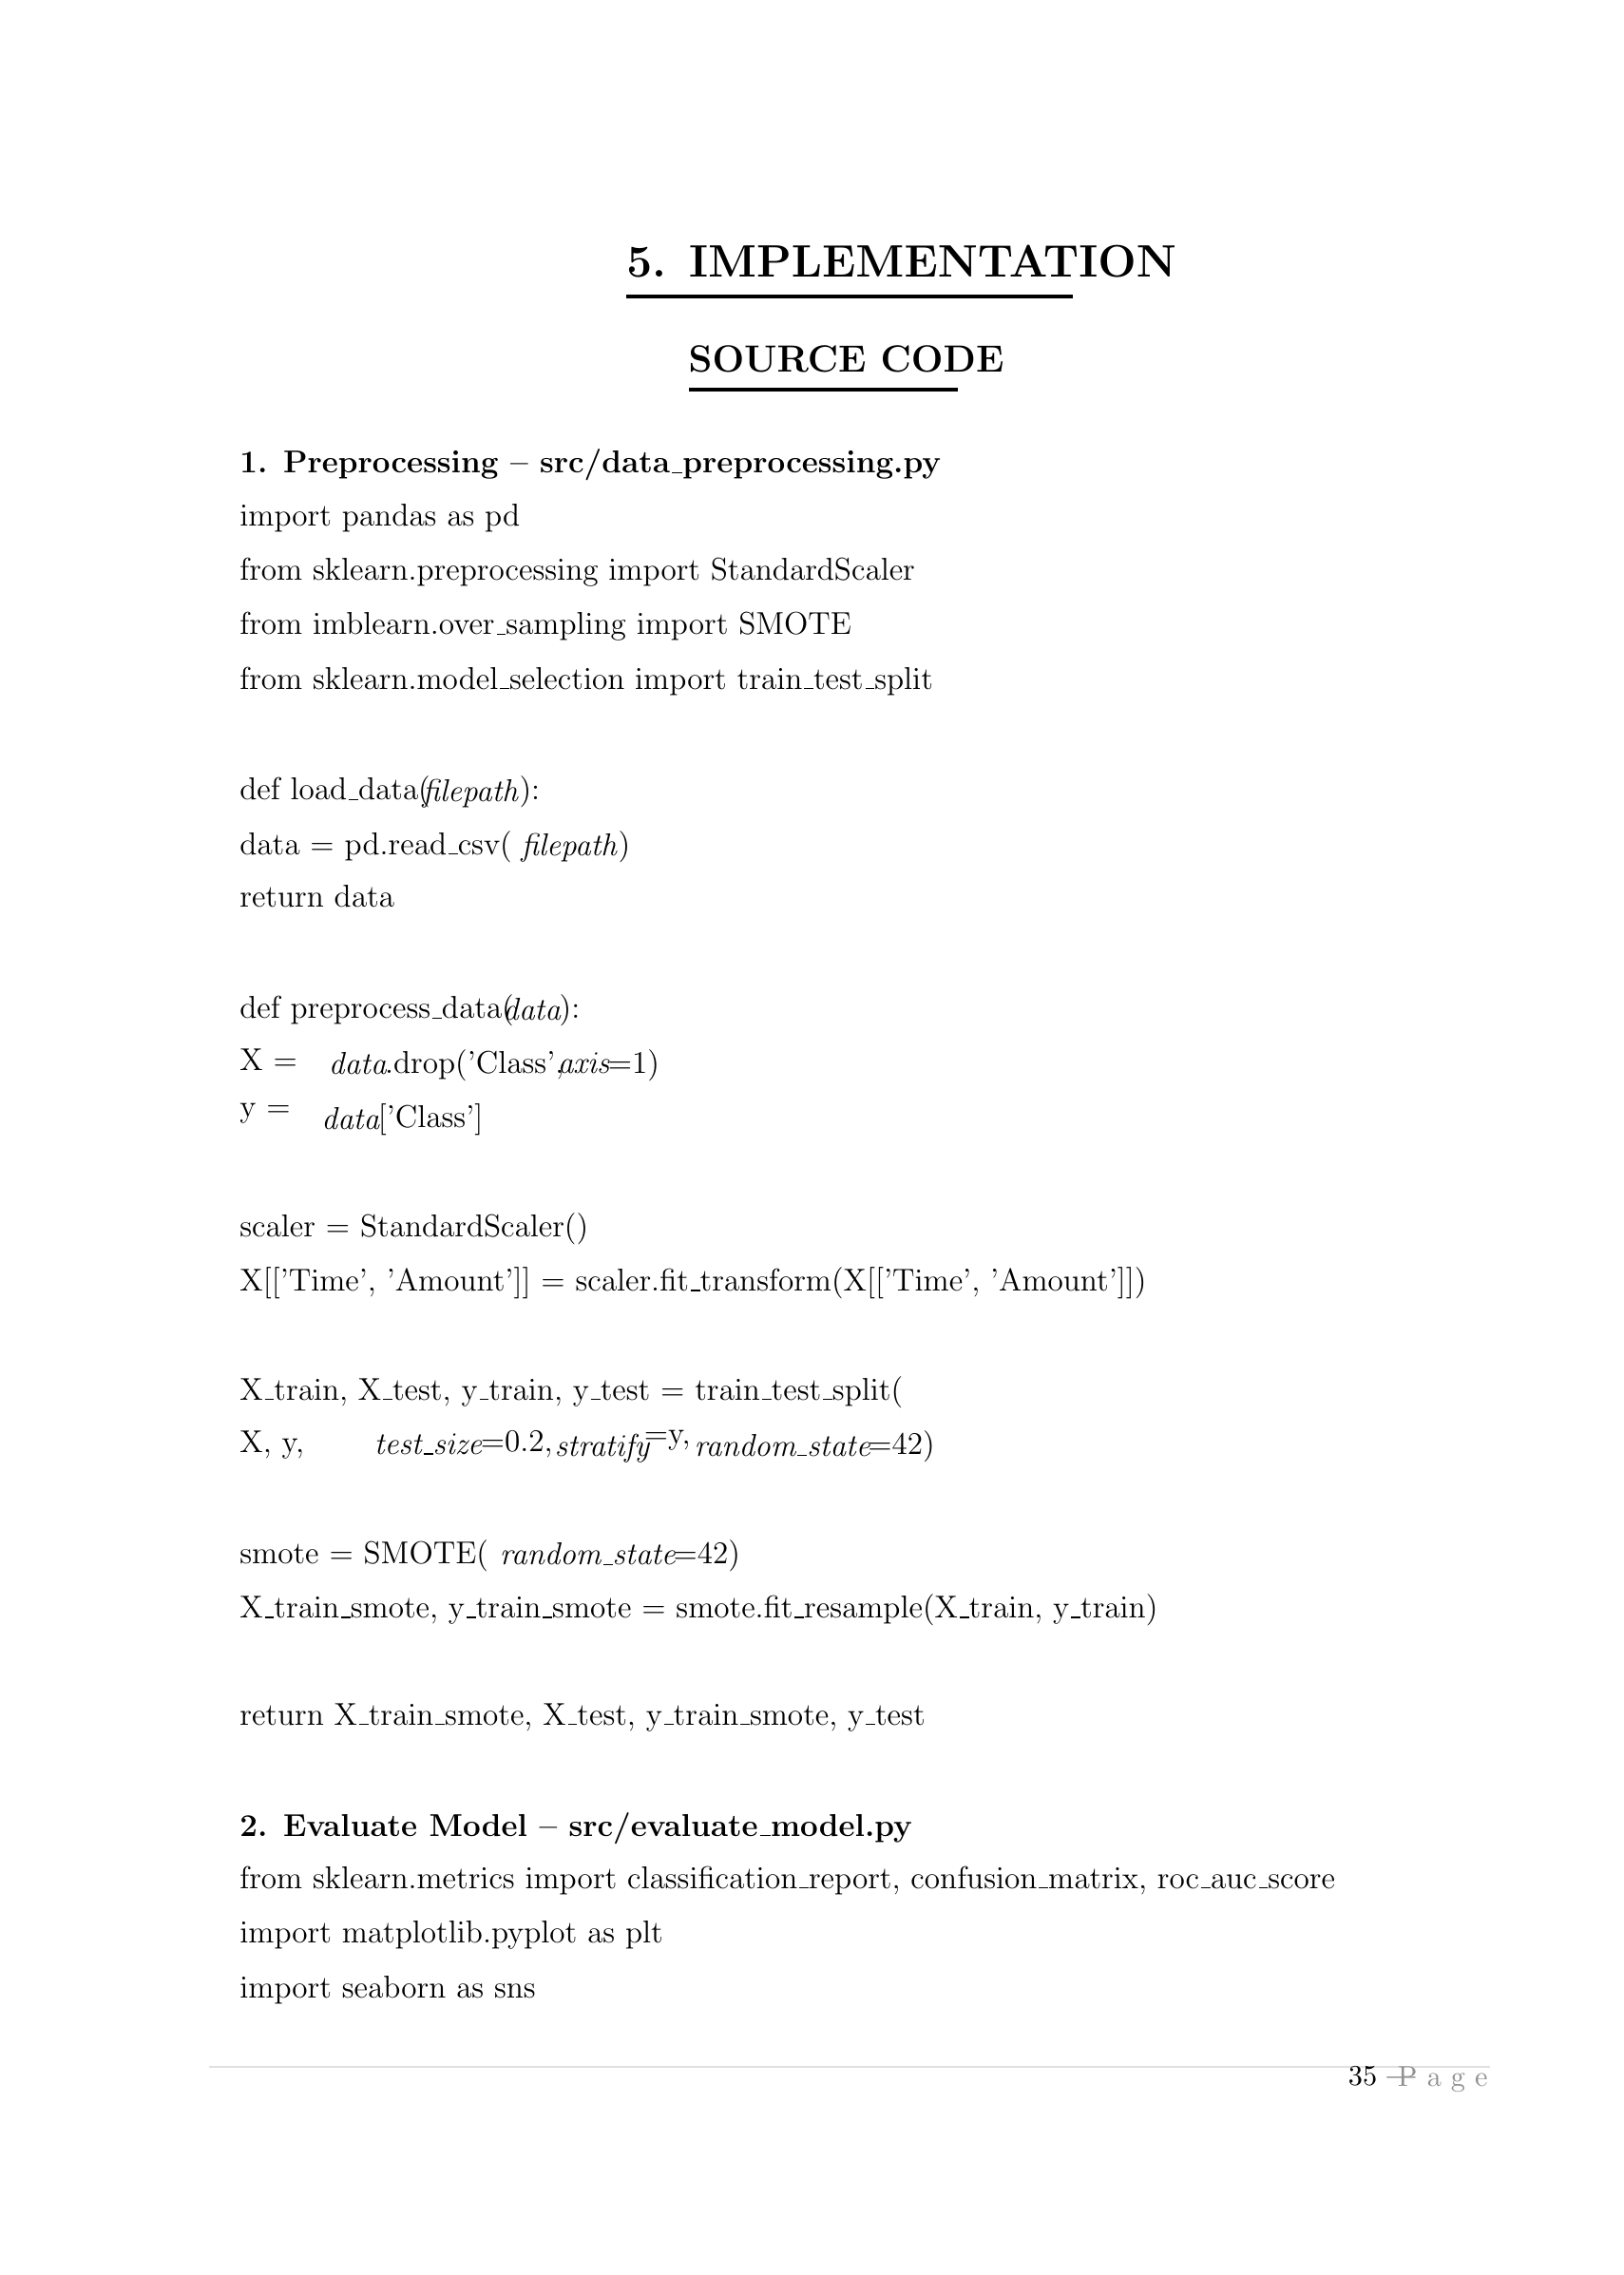
\begin{tikzpicture}[x=1bp,y=-1bp,inner sep=0pt,outer sep=0pt]
  \useasboundingbox (0,0) rectangle (595.20,841.92);
  \fill[fill=pdfcolor9] (69.38,772.78) rectangle (554.40,773.26);
  \fill[fill=black] (227.38,101.78) rectangle (396.41,103.22);
  \fill[fill=black] (250.90,137.09) rectangle (352.95,138.53);
  \node[anchor=north west,inner sep=0pt,outer sep=0pt] at (500.86,772.91) {{\fontsize{11.0bp}{13.2bp}\selectfont 35 | }};
  \node[anchor=north west,inner sep=0pt,outer sep=0pt] at (519.58,772.91) {{\fontsize{11.0bp}{13.2bp}\selectfont \textcolor{pdfcolor1}{P a g e}}};
  \node[anchor=north west,inner sep=0pt,outer sep=0pt] at (550.14,772.91) {{\fontsize{11.0bp}{13.2bp}\selectfont   }};
  \node[anchor=north west,inner sep=0pt,outer sep=0pt] at (227.38,83.31) {{\fontsize{16.1bp}{19.3bp}\selectfont \textbf{5. IMPLEMENTATION }}};
  \node[anchor=north west,inner sep=0pt,outer sep=0pt] at (70.82,124.02) {{\fontsize{11.0bp}{13.2bp}\selectfont     }};
  \node[anchor=north west,inner sep=0pt,outer sep=0pt] at (81.86,123.12) {{\fontsize{12.0bp}{14.4bp}\selectfont \textbf{ }}};
  \node[anchor=north west,inner sep=0pt,outer sep=0pt] at (106.85,123.12) {{\fontsize{12.0bp}{14.4bp}\selectfont \textbf{ }}};
  \node[anchor=north west,inner sep=0pt,outer sep=0pt] at (142.87,123.12) {{\fontsize{12.0bp}{14.4bp}\selectfont \textbf{ }}};
  \node[anchor=north west,inner sep=0pt,outer sep=0pt] at (178.87,123.12) {{\fontsize{12.0bp}{14.4bp}\selectfont \textbf{ }}};
  \node[anchor=north west,inner sep=0pt,outer sep=0pt] at (214.90,123.12) {{\fontsize{12.0bp}{14.4bp}\selectfont \textbf{ }}};
  \node[anchor=north west,inner sep=0pt,outer sep=0pt] at (250.90,121.12) {{\fontsize{13.9bp}{16.7bp}\selectfont \textbf{SOURCE CODE  }}};
  \node[anchor=north west,inner sep=0pt,outer sep=0pt] at (80.90,160.32) {{\fontsize{12.0bp}{14.4bp}\selectfont \textbf{1. Preprocessing -- src/data\_preprocessing.py }}};
  \node[anchor=north west,inner sep=0pt,outer sep=0pt] at (80.90,180.85) {{\fontsize{12.0bp}{14.4bp}\selectfont import pandas as pd }};
  \node[anchor=north west,inner sep=0pt,outer sep=0pt] at (80.90,201.51) {{\fontsize{12.0bp}{14.4bp}\selectfont from sklearn.preprocessing import StandardScaler }};
  \node[anchor=north west,inner sep=0pt,outer sep=0pt] at (80.90,222.15) {{\fontsize{12.0bp}{14.4bp}\selectfont from imblearn.over\_sampling import SMOTE }};
  \node[anchor=north west,inner sep=0pt,outer sep=0pt] at (80.90,242.79) {{\fontsize{12.0bp}{14.4bp}\selectfont from sklearn.model\_selection import train\_test\_split }};
  \node[anchor=north west,inner sep=0pt,outer sep=0pt] at (80.90,284.07) {{\fontsize{12.0bp}{14.4bp}\selectfont def load\_data(}};
  \node[anchor=north west,inner sep=0pt,outer sep=0pt] at (150.07,285.30) {{\fontsize{12.0bp}{14.4bp}\selectfont \textit{filepath}}};
  \node[anchor=north west,inner sep=0pt,outer sep=0pt] at (186.79,284.07) {{\fontsize{12.0bp}{14.4bp}\selectfont ): }};
  \node[anchor=north west,inner sep=0pt,outer sep=0pt] at (80.90,304.74) {{\fontsize{12.0bp}{14.4bp}\selectfont     data = pd.read\_csv(}};
  \node[anchor=north west,inner sep=0pt,outer sep=0pt] at (187.51,305.97) {{\fontsize{12.0bp}{14.4bp}\selectfont \textit{filepath}}};
  \node[anchor=north west,inner sep=0pt,outer sep=0pt] at (224.26,304.74) {{\fontsize{12.0bp}{14.4bp}\selectfont ) }};
  \node[anchor=north west,inner sep=0pt,outer sep=0pt] at (80.90,325.38) {{\fontsize{12.0bp}{14.4bp}\selectfont     return data }};
  \node[anchor=north west,inner sep=0pt,outer sep=0pt] at (80.90,366.90) {{\fontsize{12.0bp}{14.4bp}\selectfont def preprocess\_data(}};
  \node[anchor=north west,inner sep=0pt,outer sep=0pt] at (180.55,368.13) {{\fontsize{12.0bp}{14.4bp}\selectfont \textit{data}}};
  \node[anchor=north west,inner sep=0pt,outer sep=0pt] at (201.94,366.90) {{\fontsize{12.0bp}{14.4bp}\selectfont ): }};
  \node[anchor=north west,inner sep=0pt,outer sep=0pt] at (80.90,387.56) {{\fontsize{12.0bp}{14.4bp}\selectfont     X = }};
  \node[anchor=north west,inner sep=0pt,outer sep=0pt] at (114.53,388.79) {{\fontsize{12.0bp}{14.4bp}\selectfont \textit{data}}};
  \node[anchor=north west,inner sep=0pt,outer sep=0pt] at (135.89,387.56) {{\fontsize{12.0bp}{14.4bp}\selectfont .drop('Class', }};
  \node[anchor=north west,inner sep=0pt,outer sep=0pt] at (201.22,388.79) {{\fontsize{12.0bp}{14.4bp}\selectfont \textit{axis}}};
  \node[anchor=north west,inner sep=0pt,outer sep=0pt] at (220.42,387.56) {{\fontsize{12.0bp}{14.4bp}\selectfont =1) }};
  \node[anchor=north west,inner sep=0pt,outer sep=0pt] at (80.90,408.20) {{\fontsize{12.0bp}{14.4bp}\selectfont     y = }};
  \node[anchor=north west,inner sep=0pt,outer sep=0pt] at (111.89,409.43) {{\fontsize{12.0bp}{14.4bp}\selectfont \textit{data}}};
  \node[anchor=north west,inner sep=0pt,outer sep=0pt] at (133.25,408.20) {{\fontsize{12.0bp}{14.4bp}\selectfont ['Class'] }};
  \node[anchor=north west,inner sep=0pt,outer sep=0pt] at (80.90,449.48) {{\fontsize{12.0bp}{14.4bp}\selectfont     scaler = StandardScaler() }};
  \node[anchor=north west,inner sep=0pt,outer sep=0pt] at (80.90,470.14) {{\fontsize{12.0bp}{14.4bp}\selectfont     X[['Time', 'Amount']] = scaler.fit\_transform(X[['Time', 'Amount']]) }};
  \node[anchor=north west,inner sep=0pt,outer sep=0pt] at (80.90,511.42) {{\fontsize{12.0bp}{14.4bp}\selectfont     X\_train, X\_test, y\_train, y\_test = train\_test\_split( }};
  \node[anchor=north west,inner sep=0pt,outer sep=0pt] at (80.90,532.06) {{\fontsize{12.0bp}{14.4bp}\selectfont         X, y, }};
  \node[anchor=north west,inner sep=0pt,outer sep=0pt] at (131.81,533.29) {{\fontsize{12.0bp}{14.4bp}\selectfont \textit{test\_size}}};
  \node[anchor=north west,inner sep=0pt,outer sep=0pt] at (172.15,532.06) {{\fontsize{12.0bp}{14.4bp}\selectfont =0.2, }};
  \node[anchor=north west,inner sep=0pt,outer sep=0pt] at (200.26,533.29) {{\fontsize{12.0bp}{14.4bp}\selectfont \textit{stratify}}};
  \node[anchor=north west,inner sep=0pt,outer sep=0pt] at (234.10,532.06) {{\fontsize{12.0bp}{14.4bp}\selectfont =y, }};
  \node[anchor=north west,inner sep=0pt,outer sep=0pt] at (253.08,533.29) {{\fontsize{12.0bp}{14.4bp}\selectfont \textit{random\_state}}};
  \node[anchor=north west,inner sep=0pt,outer sep=0pt] at (318.86,532.06) {{\fontsize{12.0bp}{14.4bp}\selectfont =42) }};
  \node[anchor=north west,inner sep=0pt,outer sep=0pt] at (80.90,573.37) {{\fontsize{12.0bp}{14.4bp}\selectfont     smote = SMOTE(}};
  \node[anchor=north west,inner sep=0pt,outer sep=0pt] at (179.35,574.60) {{\fontsize{12.0bp}{14.4bp}\selectfont \textit{random\_state}}};
  \node[anchor=north west,inner sep=0pt,outer sep=0pt] at (245.14,573.37) {{\fontsize{12.0bp}{14.4bp}\selectfont =42) }};
  \node[anchor=north west,inner sep=0pt,outer sep=0pt] at (80.90,594.01) {{\fontsize{12.0bp}{14.4bp}\selectfont     X\_train\_smote, y\_train\_smote = smote.fit\_resample(X\_train, y\_train) }};
  \node[anchor=north west,inner sep=0pt,outer sep=0pt] at (80.90,635.31) {{\fontsize{12.0bp}{14.4bp}\selectfont     return X\_train\_smote, X\_test, y\_train\_smote, y\_test }};
  \node[anchor=north west,inner sep=0pt,outer sep=0pt] at (80.90,676.70) {{\fontsize{12.0bp}{14.4bp}\selectfont \textbf{2. Evaluate Model -- src/evaluate\_model.py }}};
  \node[anchor=north west,inner sep=0pt,outer sep=0pt] at (80.90,697.23) {{\fontsize{12.0bp}{14.4bp}\selectfont from sklearn.metrics import classification\_report, confusion\_matrix, roc\_auc\_score }};
  \node[anchor=north west,inner sep=0pt,outer sep=0pt] at (80.90,717.90) {{\fontsize{12.0bp}{14.4bp}\selectfont import matplotlib.pyplot as plt }};
  \node[anchor=north west,inner sep=0pt,outer sep=0pt] at (80.90,738.54) {{\fontsize{12.0bp}{14.4bp}\selectfont import seaborn as sns }};
\end{tikzpicture}
\newpage
\noindent
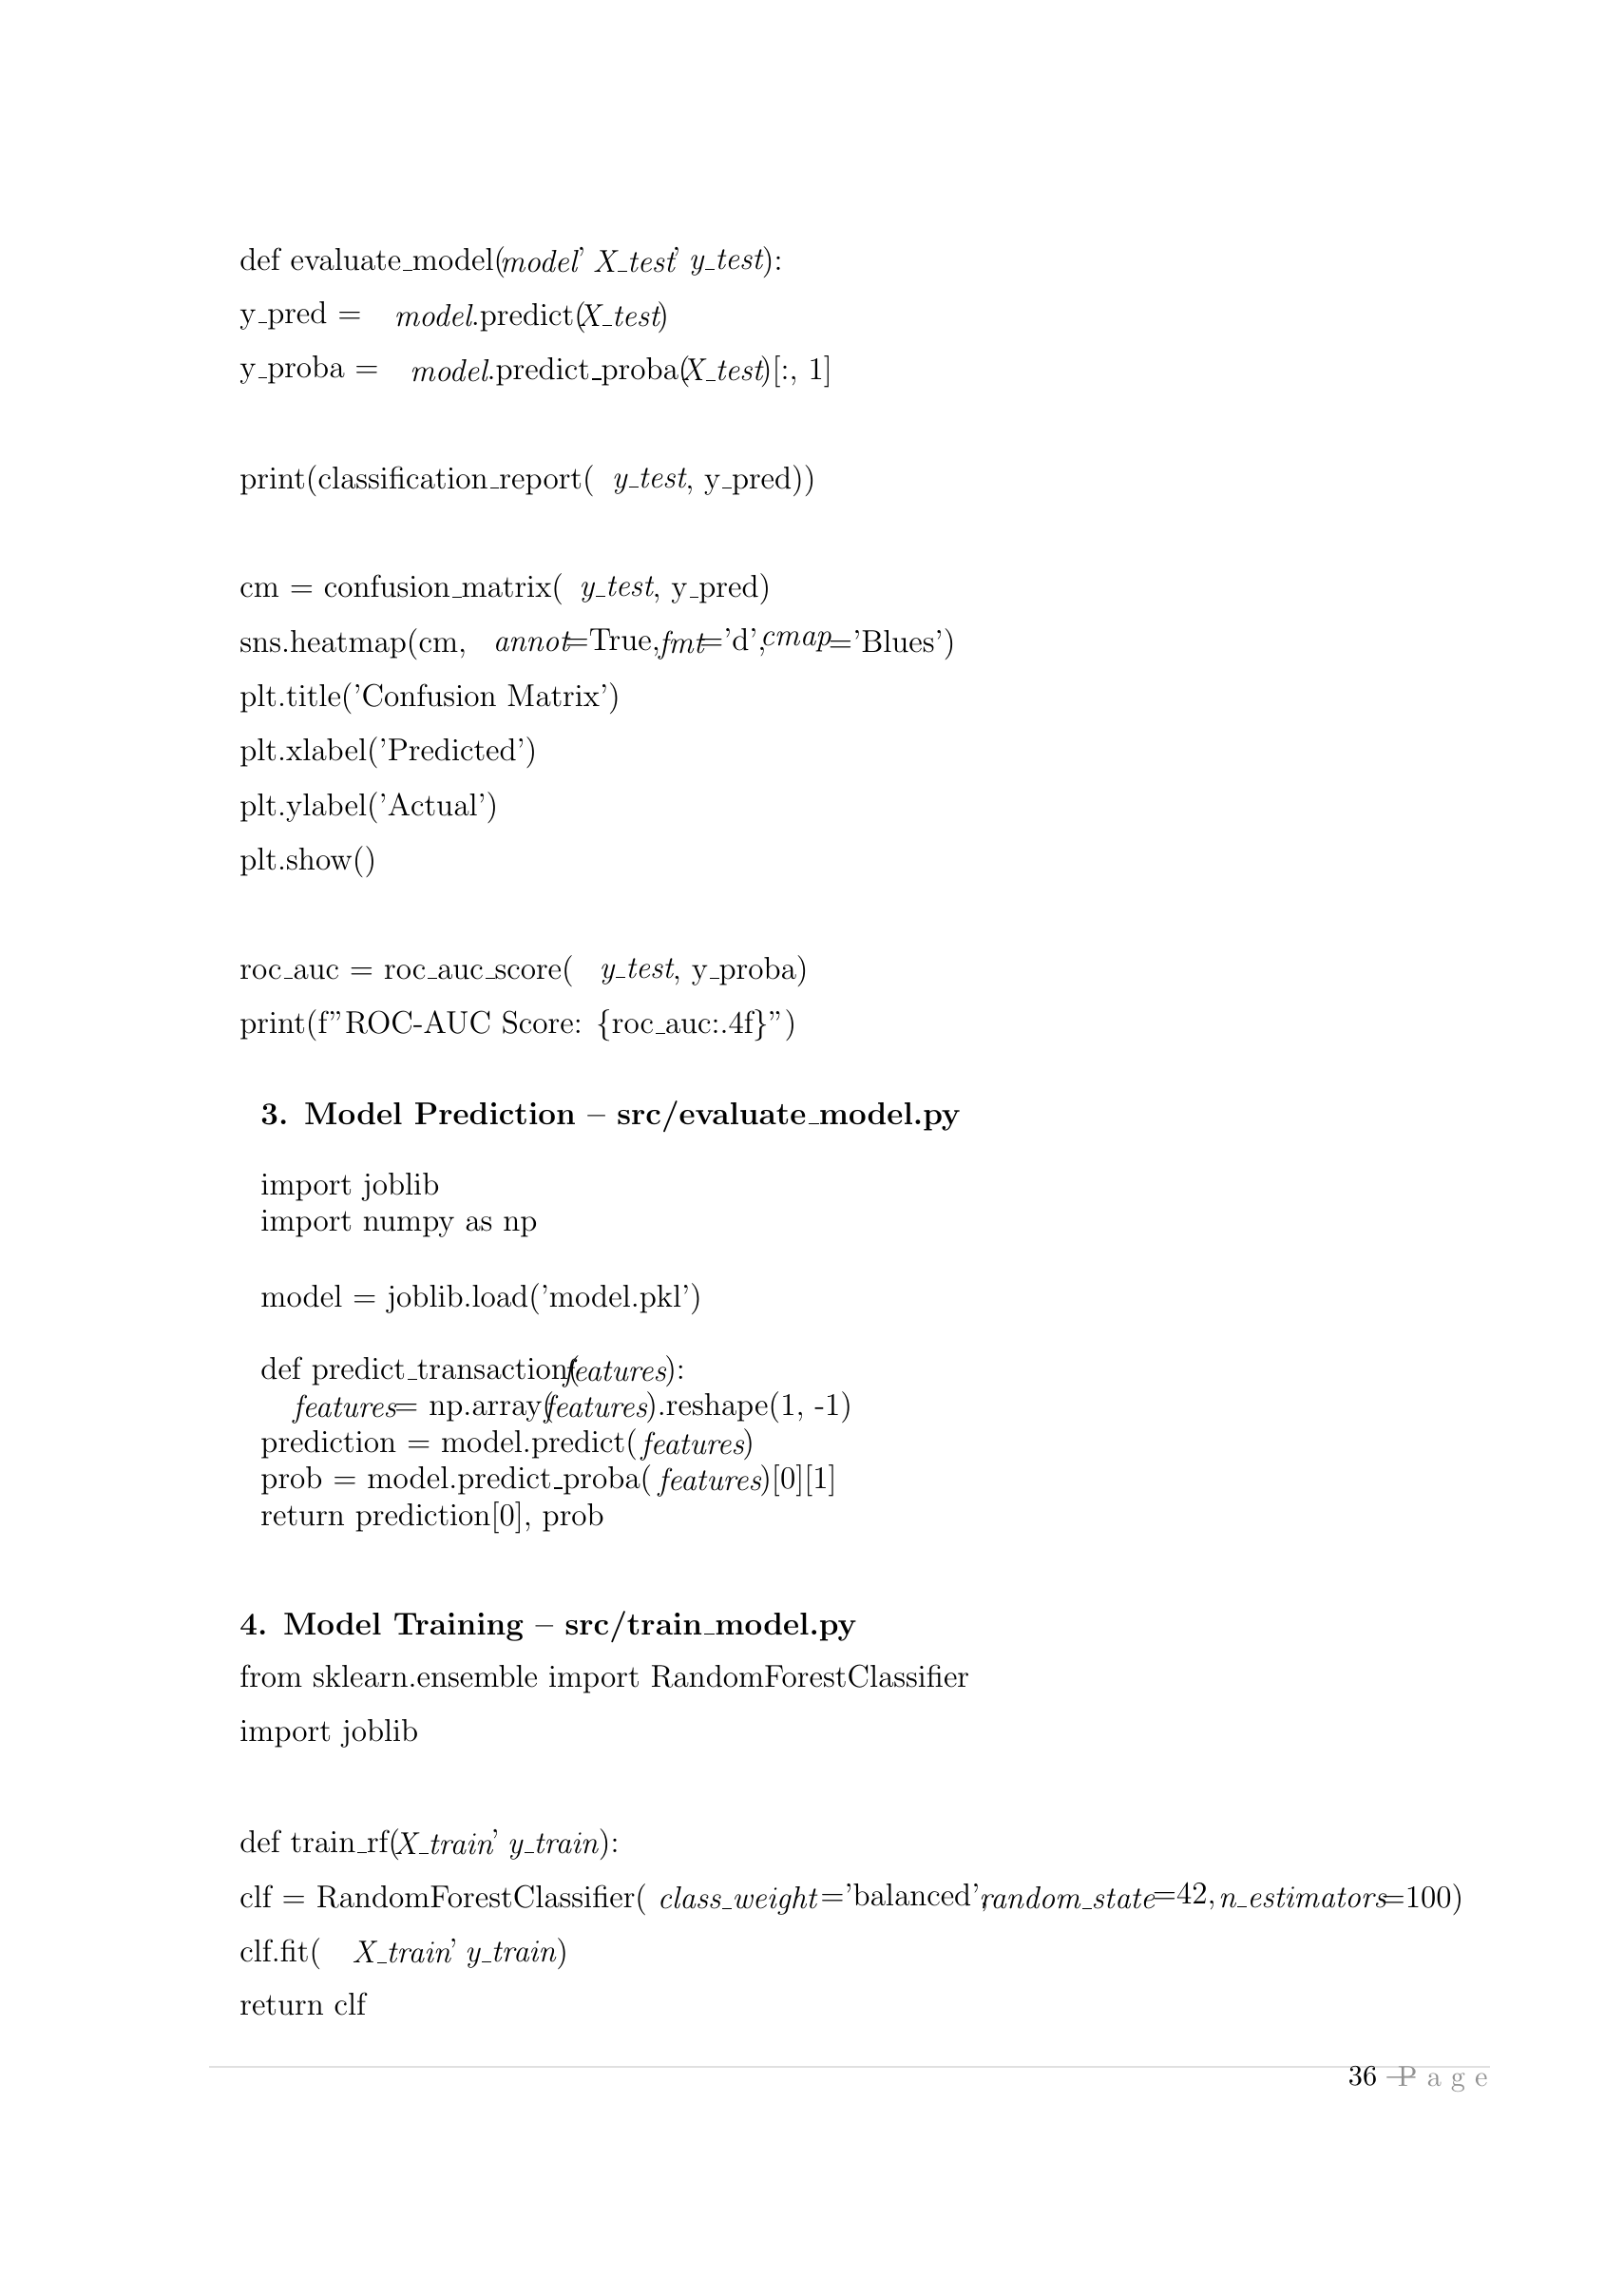
\begin{tikzpicture}[x=1bp,y=-1bp,inner sep=0pt,outer sep=0pt]
  \useasboundingbox (0,0) rectangle (595.20,841.92);
  \fill[fill=pdfcolor9] (69.38,772.78) rectangle (554.40,773.26);
  \node[anchor=north west,inner sep=0pt,outer sep=0pt] at (500.86,772.91) {{\fontsize{11.0bp}{13.2bp}\selectfont 36 | }};
  \node[anchor=north west,inner sep=0pt,outer sep=0pt] at (519.58,772.91) {{\fontsize{11.0bp}{13.2bp}\selectfont \textcolor{pdfcolor1}{P a g e}}};
  \node[anchor=north west,inner sep=0pt,outer sep=0pt] at (550.14,772.91) {{\fontsize{11.0bp}{13.2bp}\selectfont   }};
  \node[anchor=north west,inner sep=0pt,outer sep=0pt] at (80.90,83.62) {{\fontsize{12.0bp}{14.4bp}\selectfont def evaluate\_model(}};
  \node[anchor=north west,inner sep=0pt,outer sep=0pt] at (179.35,84.85) {{\fontsize{12.0bp}{14.4bp}\selectfont \textit{model}}};
  \node[anchor=north west,inner sep=0pt,outer sep=0pt] at (208.66,83.62) {{\fontsize{12.0bp}{14.4bp}\selectfont , }};
  \node[anchor=north west,inner sep=0pt,outer sep=0pt] at (214.66,84.85) {{\fontsize{12.0bp}{14.4bp}\selectfont \textit{X\_test}}};
  \node[anchor=north west,inner sep=0pt,outer sep=0pt] at (244.66,83.62) {{\fontsize{12.0bp}{14.4bp}\selectfont , }};
  \node[anchor=north west,inner sep=0pt,outer sep=0pt] at (250.90,84.85) {{\fontsize{12.0bp}{14.4bp}\selectfont \textit{y\_test}}};
  \node[anchor=north west,inner sep=0pt,outer sep=0pt] at (278.76,83.62) {{\fontsize{12.0bp}{14.4bp}\selectfont ): }};
  \node[anchor=north west,inner sep=0pt,outer sep=0pt] at (80.90,104.26) {{\fontsize{12.0bp}{14.4bp}\selectfont     y\_pred = }};
  \node[anchor=north west,inner sep=0pt,outer sep=0pt] at (139.27,105.49) {{\fontsize{12.0bp}{14.4bp}\selectfont \textit{model}}};
  \node[anchor=north west,inner sep=0pt,outer sep=0pt] at (168.55,104.26) {{\fontsize{12.0bp}{14.4bp}\selectfont .predict(}};
  \node[anchor=north west,inner sep=0pt,outer sep=0pt] at (208.90,105.49) {{\fontsize{12.0bp}{14.4bp}\selectfont \textit{X\_test}}};
  \node[anchor=north west,inner sep=0pt,outer sep=0pt] at (238.90,104.26) {{\fontsize{12.0bp}{14.4bp}\selectfont ) }};
  \node[anchor=north west,inner sep=0pt,outer sep=0pt] at (80.90,124.93) {{\fontsize{12.0bp}{14.4bp}\selectfont     y\_proba = }};
  \node[anchor=north west,inner sep=0pt,outer sep=0pt] at (145.27,126.16) {{\fontsize{12.0bp}{14.4bp}\selectfont \textit{model}}};
  \node[anchor=north west,inner sep=0pt,outer sep=0pt] at (174.55,124.93) {{\fontsize{12.0bp}{14.4bp}\selectfont .predict\_proba(}};
  \node[anchor=north west,inner sep=0pt,outer sep=0pt] at (248.02,126.16) {{\fontsize{12.0bp}{14.4bp}\selectfont \textit{X\_test}}};
  \node[anchor=north west,inner sep=0pt,outer sep=0pt] at (278.04,124.93) {{\fontsize{12.0bp}{14.4bp}\selectfont )[:, 1] }};
  \node[anchor=north west,inner sep=0pt,outer sep=0pt] at (80.90,166.21) {{\fontsize{12.0bp}{14.4bp}\selectfont     print(classification\_report(}};
  \node[anchor=north west,inner sep=0pt,outer sep=0pt] at (221.86,167.44) {{\fontsize{12.0bp}{14.4bp}\selectfont \textit{y\_test}}};
  \node[anchor=north west,inner sep=0pt,outer sep=0pt] at (249.70,166.21) {{\fontsize{12.0bp}{14.4bp}\selectfont , y\_pred)) }};
  \node[anchor=north west,inner sep=0pt,outer sep=0pt] at (80.90,207.51) {{\fontsize{12.0bp}{14.4bp}\selectfont     cm = confusion\_matrix(}};
  \node[anchor=north west,inner sep=0pt,outer sep=0pt] at (209.38,208.74) {{\fontsize{12.0bp}{14.4bp}\selectfont \textit{y\_test}}};
  \node[anchor=north west,inner sep=0pt,outer sep=0pt] at (237.22,207.51) {{\fontsize{12.0bp}{14.4bp}\selectfont , y\_pred) }};
  \node[anchor=north west,inner sep=0pt,outer sep=0pt] at (80.90,228.15) {{\fontsize{12.0bp}{14.4bp}\selectfont     sns.heatmap(cm, }};
  \node[anchor=north west,inner sep=0pt,outer sep=0pt] at (176.71,229.38) {{\fontsize{12.0bp}{14.4bp}\selectfont \textit{annot}}};
  \node[anchor=north west,inner sep=0pt,outer sep=0pt] at (204.10,228.15) {{\fontsize{12.0bp}{14.4bp}\selectfont =True, }};
  \node[anchor=north west,inner sep=0pt,outer sep=0pt] at (239.62,229.38) {{\fontsize{12.0bp}{14.4bp}\selectfont \textit{fmt}}};
  \node[anchor=north west,inner sep=0pt,outer sep=0pt] at (255.00,228.15) {{\fontsize{12.0bp}{14.4bp}\selectfont ='d', }};
  \node[anchor=north west,inner sep=0pt,outer sep=0pt] at (278.04,229.38) {{\fontsize{12.0bp}{14.4bp}\selectfont \textit{cmap}}};
  \node[anchor=north west,inner sep=0pt,outer sep=0pt] at (303.96,228.15) {{\fontsize{12.0bp}{14.4bp}\selectfont ='Blues') }};
  \node[anchor=north west,inner sep=0pt,outer sep=0pt] at (80.90,248.79) {{\fontsize{12.0bp}{14.4bp}\selectfont     plt.title('Confusion Matrix') }};
  \node[anchor=north west,inner sep=0pt,outer sep=0pt] at (80.90,269.43) {{\fontsize{12.0bp}{14.4bp}\selectfont     plt.xlabel('Predicted') }};
  \node[anchor=north west,inner sep=0pt,outer sep=0pt] at (80.90,290.10) {{\fontsize{12.0bp}{14.4bp}\selectfont     plt.ylabel('Actual') }};
  \node[anchor=north west,inner sep=0pt,outer sep=0pt] at (80.90,310.74) {{\fontsize{12.0bp}{14.4bp}\selectfont     plt.show() }};
  \node[anchor=north west,inner sep=0pt,outer sep=0pt] at (80.90,352.02) {{\fontsize{12.0bp}{14.4bp}\selectfont     roc\_auc = roc\_auc\_score(}};
  \node[anchor=north west,inner sep=0pt,outer sep=0pt] at (217.06,353.25) {{\fontsize{12.0bp}{14.4bp}\selectfont \textit{y\_test}}};
  \node[anchor=north west,inner sep=0pt,outer sep=0pt] at (244.90,352.02) {{\fontsize{12.0bp}{14.4bp}\selectfont , y\_proba) }};
  \node[anchor=north west,inner sep=0pt,outer sep=0pt] at (80.90,372.68) {{\fontsize{12.0bp}{14.4bp}\selectfont     print(f''ROC-AUC Score: \{roc\_auc:.4f\}'') }};
  \node[anchor=north west,inner sep=0pt,outer sep=0pt] at (88.85,407.11) {{\fontsize{12.0bp}{14.4bp}\selectfont \textbf{3. Model Prediction -- src/evaluate\_model.py }}};
  \node[anchor=north west,inner sep=0pt,outer sep=0pt] at (88.85,421.03) {{\fontsize{12.0bp}{14.4bp}\selectfont \textbf{ }}};
  \node[anchor=north west,inner sep=0pt,outer sep=0pt] at (88.85,434.60) {{\fontsize{12.0bp}{14.4bp}\selectfont import joblib }};
  \node[anchor=north west,inner sep=0pt,outer sep=0pt] at (88.85,448.52) {{\fontsize{12.0bp}{14.4bp}\selectfont import numpy as np }};
  \node[anchor=north west,inner sep=0pt,outer sep=0pt] at (88.85,462.22) {{\fontsize{12.0bp}{14.4bp}\selectfont  }};
  \node[anchor=north west,inner sep=0pt,outer sep=0pt] at (88.85,476.14) {{\fontsize{12.0bp}{14.4bp}\selectfont model = joblib.load('model.pkl') }};
  \node[anchor=north west,inner sep=0pt,outer sep=0pt] at (88.85,489.82) {{\fontsize{12.0bp}{14.4bp}\selectfont  }};
  \node[anchor=north west,inner sep=0pt,outer sep=0pt] at (88.85,503.74) {{\fontsize{12.0bp}{14.4bp}\selectfont def predict\_transaction(}};
  \node[anchor=north west,inner sep=0pt,outer sep=0pt] at (203.38,504.97) {{\fontsize{12.0bp}{14.4bp}\selectfont \textit{features}}};
  \node[anchor=north west,inner sep=0pt,outer sep=0pt] at (241.78,503.74) {{\fontsize{12.0bp}{14.4bp}\selectfont ): }};
  \node[anchor=north west,inner sep=0pt,outer sep=0pt] at (88.85,517.42) {{\fontsize{12.0bp}{14.4bp}\selectfont     }};
  \node[anchor=north west,inner sep=0pt,outer sep=0pt] at (101.09,518.65) {{\fontsize{12.0bp}{14.4bp}\selectfont \textit{features}}};
  \node[anchor=north west,inner sep=0pt,outer sep=0pt] at (139.51,517.42) {{\fontsize{12.0bp}{14.4bp}\selectfont  = np.array(}};
  \node[anchor=north west,inner sep=0pt,outer sep=0pt] at (196.18,518.65) {{\fontsize{12.0bp}{14.4bp}\selectfont \textit{features}}};
  \node[anchor=north west,inner sep=0pt,outer sep=0pt] at (234.58,517.42) {{\fontsize{12.0bp}{14.4bp}\selectfont ).reshape(1, -1) }};
  \node[anchor=north west,inner sep=0pt,outer sep=0pt] at (88.85,531.34) {{\fontsize{12.0bp}{14.4bp}\selectfont     prediction = model.predict(}};
  \node[anchor=north west,inner sep=0pt,outer sep=0pt] at (232.90,532.57) {{\fontsize{12.0bp}{14.4bp}\selectfont \textit{features}}};
  \node[anchor=north west,inner sep=0pt,outer sep=0pt] at (271.32,531.34) {{\fontsize{12.0bp}{14.4bp}\selectfont ) }};
  \node[anchor=north west,inner sep=0pt,outer sep=0pt] at (88.85,545.05) {{\fontsize{12.0bp}{14.4bp}\selectfont     prob = model.predict\_proba(}};
  \node[anchor=north west,inner sep=0pt,outer sep=0pt] at (239.38,546.28) {{\fontsize{12.0bp}{14.4bp}\selectfont \textit{features}}};
  \node[anchor=north west,inner sep=0pt,outer sep=0pt] at (277.80,545.05) {{\fontsize{12.0bp}{14.4bp}\selectfont )[0][1] }};
  \node[anchor=north west,inner sep=0pt,outer sep=0pt] at (88.85,558.97) {{\fontsize{12.0bp}{14.4bp}\selectfont     return prediction[0], prob }};
  \node[anchor=north west,inner sep=0pt,outer sep=0pt] at (80.90,600.36) {{\fontsize{12.0bp}{14.4bp}\selectfont \textbf{4. Model Training -- src/train\_model.py }}};
  \node[anchor=north west,inner sep=0pt,outer sep=0pt] at (80.90,620.89) {{\fontsize{12.0bp}{14.4bp}\selectfont from sklearn.ensemble import RandomForestClassifier }};
  \node[anchor=north west,inner sep=0pt,outer sep=0pt] at (80.90,641.55) {{\fontsize{12.0bp}{14.4bp}\selectfont import joblib }};
  \node[anchor=north west,inner sep=0pt,outer sep=0pt] at (80.90,683.07) {{\fontsize{12.0bp}{14.4bp}\selectfont def train\_rf(}};
  \node[anchor=north west,inner sep=0pt,outer sep=0pt] at (139.27,684.30) {{\fontsize{12.0bp}{14.4bp}\selectfont \textit{X\_train}}};
  \node[anchor=north west,inner sep=0pt,outer sep=0pt] at (175.99,683.07) {{\fontsize{12.0bp}{14.4bp}\selectfont , }};
  \node[anchor=north west,inner sep=0pt,outer sep=0pt] at (182.23,684.30) {{\fontsize{12.0bp}{14.4bp}\selectfont \textit{y\_train}}};
  \node[anchor=north west,inner sep=0pt,outer sep=0pt] at (216.82,683.07) {{\fontsize{12.0bp}{14.4bp}\selectfont ): }};
  \node[anchor=north west,inner sep=0pt,outer sep=0pt] at (80.90,703.71) {{\fontsize{12.0bp}{14.4bp}\selectfont     clf = RandomForestClassifier(}};
  \node[anchor=north west,inner sep=0pt,outer sep=0pt] at (239.14,704.94) {{\fontsize{12.0bp}{14.4bp}\selectfont \textit{class\_weight}}};
  \node[anchor=north west,inner sep=0pt,outer sep=0pt] at (300.84,703.71) {{\fontsize{12.0bp}{14.4bp}\selectfont ='balanced', }};
  \node[anchor=north west,inner sep=0pt,outer sep=0pt] at (360.86,704.94) {{\fontsize{12.0bp}{14.4bp}\selectfont \textit{random\_state}}};
  \node[anchor=north west,inner sep=0pt,outer sep=0pt] at (426.67,703.71) {{\fontsize{12.0bp}{14.4bp}\selectfont =42, }};
  \node[anchor=north west,inner sep=0pt,outer sep=0pt] at (451.63,704.94) {{\fontsize{12.0bp}{14.4bp}\selectfont \textit{n\_estimators}}};
  \node[anchor=north west,inner sep=0pt,outer sep=0pt] at (513.34,703.71) {{\fontsize{12.0bp}{14.4bp}\selectfont =100) }};
  \node[anchor=north west,inner sep=0pt,outer sep=0pt] at (80.90,724.38) {{\fontsize{12.0bp}{14.4bp}\selectfont     clf.fit(}};
  \node[anchor=north west,inner sep=0pt,outer sep=0pt] at (123.41,725.61) {{\fontsize{12.0bp}{14.4bp}\selectfont \textit{X\_train}}};
  \node[anchor=north west,inner sep=0pt,outer sep=0pt] at (160.15,724.38) {{\fontsize{12.0bp}{14.4bp}\selectfont , }};
  \node[anchor=north west,inner sep=0pt,outer sep=0pt] at (166.15,725.61) {{\fontsize{12.0bp}{14.4bp}\selectfont \textit{y\_train}}};
  \node[anchor=north west,inner sep=0pt,outer sep=0pt] at (200.74,724.38) {{\fontsize{12.0bp}{14.4bp}\selectfont ) }};
  \node[anchor=north west,inner sep=0pt,outer sep=0pt] at (80.90,745.02) {{\fontsize{12.0bp}{14.4bp}\selectfont     return clf }};
\end{tikzpicture}
\newpage
\noindent
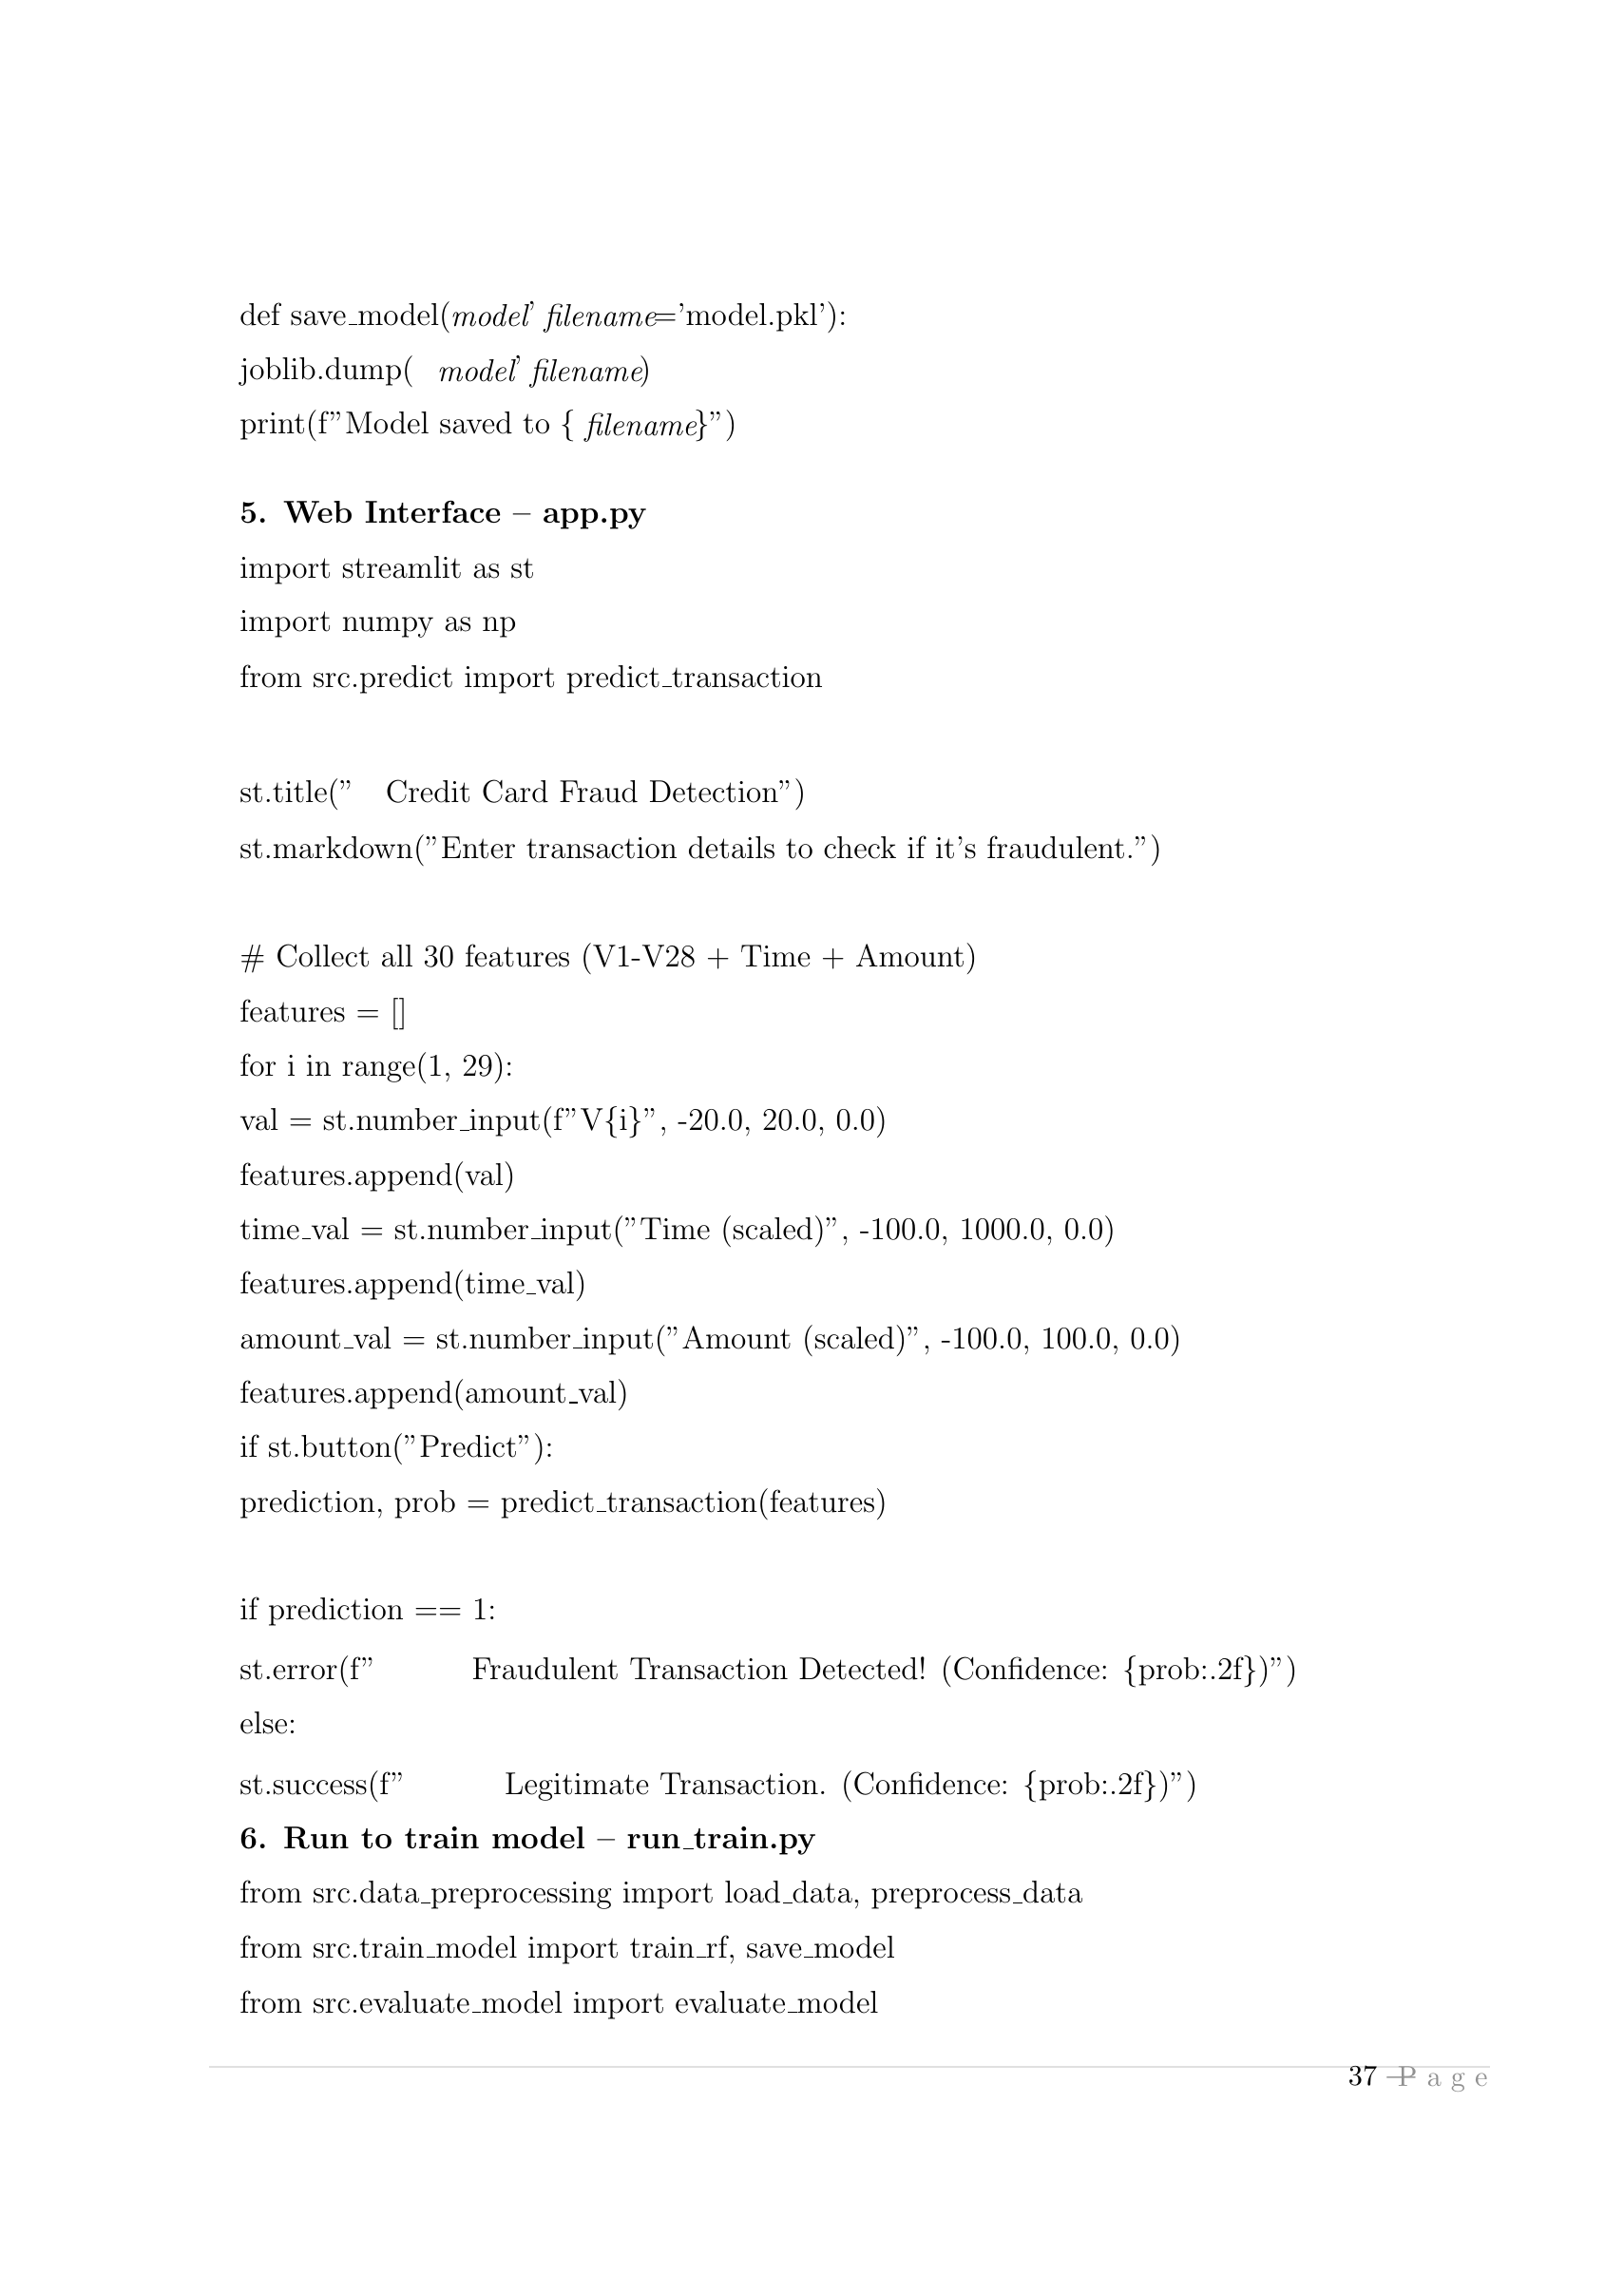
\begin{tikzpicture}[x=1bp,y=-1bp,inner sep=0pt,outer sep=0pt]
  \useasboundingbox (0,0) rectangle (595.20,841.92);
  \fill[fill=pdfcolor9] (69.38,772.78) rectangle (554.40,773.26);
  \node[anchor=north west,inner sep=0pt,outer sep=0pt] at (500.86,772.91) {{\fontsize{11.0bp}{13.2bp}\selectfont 37 | }};
  \node[anchor=north west,inner sep=0pt,outer sep=0pt] at (519.58,772.91) {{\fontsize{11.0bp}{13.2bp}\selectfont \textcolor{pdfcolor1}{P a g e}}};
  \node[anchor=north west,inner sep=0pt,outer sep=0pt] at (550.14,772.91) {{\fontsize{11.0bp}{13.2bp}\selectfont   }};
  \node[anchor=north west,inner sep=0pt,outer sep=0pt] at (80.90,104.26) {{\fontsize{12.0bp}{14.4bp}\selectfont def save\_model(}};
  \node[anchor=north west,inner sep=0pt,outer sep=0pt] at (160.63,105.49) {{\fontsize{12.0bp}{14.4bp}\selectfont \textit{model}}};
  \node[anchor=north west,inner sep=0pt,outer sep=0pt] at (189.91,104.26) {{\fontsize{12.0bp}{14.4bp}\selectfont , }};
  \node[anchor=north west,inner sep=0pt,outer sep=0pt] at (196.18,105.49) {{\fontsize{12.0bp}{14.4bp}\selectfont \textit{filename}}};
  \node[anchor=north west,inner sep=0pt,outer sep=0pt] at (237.46,104.26) {{\fontsize{12.0bp}{14.4bp}\selectfont ='model.pkl'): }};
  \node[anchor=north west,inner sep=0pt,outer sep=0pt] at (80.90,124.93) {{\fontsize{12.0bp}{14.4bp}\selectfont     joblib.dump(}};
  \node[anchor=north west,inner sep=0pt,outer sep=0pt] at (155.59,126.16) {{\fontsize{12.0bp}{14.4bp}\selectfont \textit{model}}};
  \node[anchor=north west,inner sep=0pt,outer sep=0pt] at (184.63,124.93) {{\fontsize{12.0bp}{14.4bp}\selectfont , }};
  \node[anchor=north west,inner sep=0pt,outer sep=0pt] at (190.87,126.16) {{\fontsize{12.0bp}{14.4bp}\selectfont \textit{filename}}};
  \node[anchor=north west,inner sep=0pt,outer sep=0pt] at (232.18,124.93) {{\fontsize{12.0bp}{14.4bp}\selectfont ) }};
  \node[anchor=north west,inner sep=0pt,outer sep=0pt] at (80.90,145.57) {{\fontsize{12.0bp}{14.4bp}\selectfont     print(f''Model saved to \{}};
  \node[anchor=north west,inner sep=0pt,outer sep=0pt] at (211.54,146.80) {{\fontsize{12.0bp}{14.4bp}\selectfont \textit{filename}}};
  \node[anchor=north west,inner sep=0pt,outer sep=0pt] at (252.84,145.57) {{\fontsize{12.0bp}{14.4bp}\selectfont \}'') }};
  \node[anchor=north west,inner sep=0pt,outer sep=0pt] at (80.90,180.00) {{\fontsize{12.0bp}{14.4bp}\selectfont \textbf{5. Web Interface -- app.py }}};
  \node[anchor=north west,inner sep=0pt,outer sep=0pt] at (80.90,200.79) {{\fontsize{12.0bp}{14.4bp}\selectfont import streamlit as st }};
  \node[anchor=north west,inner sep=0pt,outer sep=0pt] at (80.90,221.43) {{\fontsize{12.0bp}{14.4bp}\selectfont import numpy as np }};
  \node[anchor=north west,inner sep=0pt,outer sep=0pt] at (80.90,242.07) {{\fontsize{12.0bp}{14.4bp}\selectfont from src.predict import predict\_transaction }};
  \node[anchor=north west,inner sep=0pt,outer sep=0pt] at (80.90,285.03) {{\fontsize{12.0bp}{14.4bp}\selectfont st.title(''}};
  \node[anchor=north west,inner sep=0pt,outer sep=0pt] at (119.57,288.36) {\textsf{{\fontsize{12.0bp}{14.4bp}\selectfont \textcolor{pdfcolor2}{ }}}};
  \node[anchor=north west,inner sep=0pt,outer sep=0pt] at (136.13,285.03) {{\fontsize{12.0bp}{14.4bp}\selectfont  Credit Card Fraud Detection'') }};
  \node[anchor=north west,inner sep=0pt,outer sep=0pt] at (80.90,306.18) {{\fontsize{12.0bp}{14.4bp}\selectfont st.markdown(''Enter transaction details to check if it's fraudulent.'') }};
  \node[anchor=north west,inner sep=0pt,outer sep=0pt] at (80.90,347.46) {{\fontsize{12.0bp}{14.4bp}\selectfont \# Collect all 30 features (V1-V28 + Time + Amount) }};
  \node[anchor=north west,inner sep=0pt,outer sep=0pt] at (80.90,368.10) {{\fontsize{12.0bp}{14.4bp}\selectfont features = [] }};
  \node[anchor=north west,inner sep=0pt,outer sep=0pt] at (80.90,388.76) {{\fontsize{12.0bp}{14.4bp}\selectfont for i in range(1, 29): }};
  \node[anchor=north west,inner sep=0pt,outer sep=0pt] at (80.90,409.40) {{\fontsize{12.0bp}{14.4bp}\selectfont     val = st.number\_input(f''V\{i\}'', -20.0, 20.0, 0.0) }};
  \node[anchor=north west,inner sep=0pt,outer sep=0pt] at (80.90,430.04) {{\fontsize{12.0bp}{14.4bp}\selectfont     features.append(val) }};
  \node[anchor=north west,inner sep=0pt,outer sep=0pt] at (80.90,450.68) {{\fontsize{12.0bp}{14.4bp}\selectfont time\_val = st.number\_input(''Time (scaled)'', -100.0, 1000.0, 0.0) }};
  \node[anchor=north west,inner sep=0pt,outer sep=0pt] at (80.90,471.34) {{\fontsize{12.0bp}{14.4bp}\selectfont features.append(time\_val) }};
  \node[anchor=north west,inner sep=0pt,outer sep=0pt] at (80.90,491.98) {{\fontsize{12.0bp}{14.4bp}\selectfont amount\_val = st.number\_input(''Amount (scaled)'', -100.0, 100.0, 0.0) }};
  \node[anchor=north west,inner sep=0pt,outer sep=0pt] at (80.90,512.62) {{\fontsize{12.0bp}{14.4bp}\selectfont features.append(amount\_val) }};
  \node[anchor=north west,inner sep=0pt,outer sep=0pt] at (80.90,533.26) {{\fontsize{12.0bp}{14.4bp}\selectfont if st.button(''Predict''): }};
  \node[anchor=north west,inner sep=0pt,outer sep=0pt] at (80.90,553.93) {{\fontsize{12.0bp}{14.4bp}\selectfont     prediction, prob = predict\_transaction(features) }};
  \node[anchor=north west,inner sep=0pt,outer sep=0pt] at (80.90,595.21) {{\fontsize{12.0bp}{14.4bp}\selectfont     if prediction == 1: }};
  \node[anchor=north west,inner sep=0pt,outer sep=0pt] at (80.90,617.53) {{\fontsize{12.0bp}{14.4bp}\selectfont         st.error(f''}};
  \node[anchor=north west,inner sep=0pt,outer sep=0pt] at (152.23,620.86) {\textsf{{\fontsize{12.0bp}{14.4bp}\selectfont \textcolor{pdfcolor3}{ }}}};
  \node[anchor=north west,inner sep=0pt,outer sep=0pt] at (168.79,617.53) {{\fontsize{12.0bp}{14.4bp}\selectfont  Fraudulent Transaction Detected! (Confidence: \{prob:.2f\})'') }};
  \node[anchor=north west,inner sep=0pt,outer sep=0pt] at (80.90,638.67) {{\fontsize{12.0bp}{14.4bp}\selectfont     else: }};
  \node[anchor=north west,inner sep=0pt,outer sep=0pt] at (80.90,660.99) {{\fontsize{12.0bp}{14.4bp}\selectfont         st.success(f''}};
  \node[anchor=north west,inner sep=0pt,outer sep=0pt] at (164.71,664.32) {\textsf{{\fontsize{12.0bp}{14.4bp}\selectfont \textcolor{pdfcolor4}{ }}}};
  \node[anchor=north west,inner sep=0pt,outer sep=0pt] at (181.27,660.99) {{\fontsize{12.0bp}{14.4bp}\selectfont  Legitimate Transaction. (Confidence: \{prob:.2f\})'') }};
  \node[anchor=north west,inner sep=0pt,outer sep=0pt] at (80.90,682.22) {{\fontsize{12.0bp}{14.4bp}\selectfont \textbf{6. Run to train model -- run\_train.py }}};
  \node[anchor=north west,inner sep=0pt,outer sep=0pt] at (80.90,702.75) {{\fontsize{12.0bp}{14.4bp}\selectfont from src.data\_preprocessing import load\_data, preprocess\_data }};
  \node[anchor=north west,inner sep=0pt,outer sep=0pt] at (80.90,723.42) {{\fontsize{12.0bp}{14.4bp}\selectfont from src.train\_model import train\_rf, save\_model }};
  \node[anchor=north west,inner sep=0pt,outer sep=0pt] at (80.90,744.30) {{\fontsize{12.0bp}{14.4bp}\selectfont from src.evaluate\_model import evaluate\_model }};
\end{tikzpicture}
\newpage
\noindent
\begin{tikzpicture}[x=1bp,y=-1bp,inner sep=0pt,outer sep=0pt]
  \useasboundingbox (0,0) rectangle (595.20,841.92);
  \fill[fill=pdfcolor9] (69.38,772.78) rectangle (554.40,773.26);
  \node[anchor=north west,inner sep=0pt,outer sep=0pt] at (500.86,772.91) {{\fontsize{11.0bp}{13.2bp}\selectfont 38 | }};
  \node[anchor=north west,inner sep=0pt,outer sep=0pt] at (519.58,772.91) {{\fontsize{11.0bp}{13.2bp}\selectfont \textcolor{pdfcolor1}{P a g e}}};
  \node[anchor=north west,inner sep=0pt,outer sep=0pt] at (550.14,772.91) {{\fontsize{11.0bp}{13.2bp}\selectfont   }};
  \node[anchor=north west,inner sep=0pt,outer sep=0pt] at (80.90,104.26) {{\fontsize{12.0bp}{14.4bp}\selectfont def main(): }};
  \node[anchor=north west,inner sep=0pt,outer sep=0pt] at (80.90,126.61) {{\fontsize{12.0bp}{14.4bp}\selectfont     print(''}};
  \node[anchor=north west,inner sep=0pt,outer sep=0pt] at (124.61,129.94) {\textsf{{\fontsize{12.0bp}{14.4bp}\selectfont \textcolor{pdfcolor4}{ }}}};
  \node[anchor=north west,inner sep=0pt,outer sep=0pt] at (141.19,126.61) {{\fontsize{12.0bp}{14.4bp}\selectfont  Script started'') }};
  \node[anchor=north west,inner sep=0pt,outer sep=0pt] at (80.90,168.37) {{\fontsize{12.0bp}{14.4bp}\selectfont     data\_path = 'data/creditcard.csv' }};
  \node[anchor=north west,inner sep=0pt,outer sep=0pt] at (80.90,190.69) {{\fontsize{12.0bp}{14.4bp}\selectfont     print(''}};
  \node[anchor=north west,inner sep=0pt,outer sep=0pt] at (124.61,194.02) {\textsf{{\fontsize{12.0bp}{14.4bp}\selectfont \textcolor{pdfcolor5}{ }}}};
  \node[anchor=north west,inner sep=0pt,outer sep=0pt] at (141.19,190.69) {{\fontsize{12.0bp}{14.4bp}\selectfont  Loading data...'') }};
  \node[anchor=north west,inner sep=0pt,outer sep=0pt] at (80.90,211.83) {{\fontsize{12.0bp}{14.4bp}\selectfont     data = load\_data(data\_path) }};
  \node[anchor=north west,inner sep=0pt,outer sep=0pt] at (80.90,254.79) {{\fontsize{12.0bp}{14.4bp}\selectfont     print(''}};
  \node[anchor=north west,inner sep=0pt,outer sep=0pt] at (124.61,258.12) {\textsf{{\fontsize{12.0bp}{14.4bp}\selectfont \textcolor{pdfcolor5}{ }}}};
  \node[anchor=north west,inner sep=0pt,outer sep=0pt] at (141.19,254.79) {{\fontsize{12.0bp}{14.4bp}\selectfont  Preprocessing data...'') }};
  \node[anchor=north west,inner sep=0pt,outer sep=0pt] at (80.90,275.91) {{\fontsize{12.0bp}{14.4bp}\selectfont     X\_train, X\_test, y\_train, y\_test = preprocess\_data(data) }};
  \node[anchor=north west,inner sep=0pt,outer sep=0pt] at (80.90,318.90) {{\fontsize{12.0bp}{14.4bp}\selectfont     print(''}};
  \node[anchor=north west,inner sep=0pt,outer sep=0pt] at (124.61,322.23) {\textsf{{\fontsize{12.0bp}{14.4bp}\selectfont \textcolor{pdfcolor6}{ }}}};
  \node[anchor=north west,inner sep=0pt,outer sep=0pt] at (141.19,318.90) {{\fontsize{12.0bp}{14.4bp}\selectfont  Training model...'') }};
  \node[anchor=north west,inner sep=0pt,outer sep=0pt] at (80.90,340.02) {{\fontsize{12.0bp}{14.4bp}\selectfont     model = train\_rf(X\_train, y\_train) }};
  \node[anchor=north west,inner sep=0pt,outer sep=0pt] at (80.90,362.34) {{\fontsize{12.0bp}{14.4bp}\selectfont     print(''}};
  \node[anchor=north west,inner sep=0pt,outer sep=0pt] at (124.61,365.67) {\textsf{{\fontsize{12.0bp}{14.4bp}\selectfont \textcolor{pdfcolor4}{ }}}};
  \node[anchor=north west,inner sep=0pt,outer sep=0pt] at (141.19,362.34) {{\fontsize{12.0bp}{14.4bp}\selectfont  Model training completed!'') }};
  \node[anchor=north west,inner sep=0pt,outer sep=0pt] at (80.90,405.80) {{\fontsize{12.0bp}{14.4bp}\selectfont     print(''}};
  \node[anchor=north west,inner sep=0pt,outer sep=0pt] at (124.61,409.13) {\textsf{{\fontsize{12.0bp}{14.4bp}\selectfont \textcolor{pdfcolor7}{ }}}};
  \node[anchor=north west,inner sep=0pt,outer sep=0pt] at (141.19,405.80) {{\fontsize{12.0bp}{14.4bp}\selectfont  Saving model...'') }};
  \node[anchor=north west,inner sep=0pt,outer sep=0pt] at (80.90,426.92) {{\fontsize{12.0bp}{14.4bp}\selectfont     save\_model(model) }};
  \node[anchor=north west,inner sep=0pt,outer sep=0pt] at (80.90,470.14) {{\fontsize{12.0bp}{14.4bp}\selectfont     print(''}};
  \node[anchor=north west,inner sep=0pt,outer sep=0pt] at (124.61,473.47) {\textsf{{\fontsize{12.0bp}{14.4bp}\selectfont \textcolor{pdfcolor8}{ }}}};
  \node[anchor=north west,inner sep=0pt,outer sep=0pt] at (141.19,470.14) {{\fontsize{12.0bp}{14.4bp}\selectfont  Evaluating model...'') }};
  \node[anchor=north west,inner sep=0pt,outer sep=0pt] at (80.90,491.26) {{\fontsize{12.0bp}{14.4bp}\selectfont     evaluate\_model(model, X\_test, y\_test) }};
  \node[anchor=north west,inner sep=0pt,outer sep=0pt] at (80.90,534.22) {{\fontsize{12.0bp}{14.4bp}\selectfont     print(''}};
  \node[anchor=north west,inner sep=0pt,outer sep=0pt] at (124.61,537.55) {\textsf{{\fontsize{12.0bp}{14.4bp}\selectfont \textcolor{pdfcolor4}{ }}}};
  \node[anchor=north west,inner sep=0pt,outer sep=0pt] at (141.19,534.22) {{\fontsize{12.0bp}{14.4bp}\selectfont  Executed successfully!'') }};
  \node[anchor=north west,inner sep=0pt,outer sep=0pt] at (80.90,576.01) {{\fontsize{12.0bp}{14.4bp}\selectfont if \_\_name\_\_ == ''\_\_main\_\_'': }};
  \node[anchor=north west,inner sep=0pt,outer sep=0pt] at (80.90,596.65) {{\fontsize{12.0bp}{14.4bp}\selectfont     main() }};
  \node[anchor=north west,inner sep=0pt,outer sep=0pt] at (80.90,637.95) {{\fontsize{12.0bp}{14.4bp}\selectfont These snippets collectively demonstrate the backend logic, model processing, and user interaction }};
  \node[anchor=north west,inner sep=0pt,outer sep=0pt] at (106.85,651.63) {{\fontsize{12.0bp}{14.4bp}\selectfont modules working in sync. They are derived from real files in the /src folder and follow }};
  \node[anchor=north west,inner sep=0pt,outer sep=0pt] at (106.85,665.31) {{\fontsize{12.0bp}{14.4bp}\selectfont clean, production-ready coding practices. }};
  \node[anchor=north west,inner sep=0pt] at (80.90,576.01) {$\displaystyle if __name__ == "__main__":$};
  \node[anchor=north west,inner sep=0pt] at (80.90,596.65) {$\displaystyle main()$};
\end{tikzpicture}
\newpage
\noindent
\begin{tikzpicture}[x=1bp,y=-1bp,inner sep=0pt,outer sep=0pt]
  \useasboundingbox (0,0) rectangle (595.20,841.92);
  \fill[fill=pdfcolor9] (69.38,772.78) rectangle (554.40,773.26);
  \fill[fill=black] (271.80,101.78) rectangle (351.74,103.22);
  \fill[fill=black] (159.91,139.49) rectangle (463.87,140.93);
  \node[anchor=north west,inner sep=0pt] at (70.90,197.84) {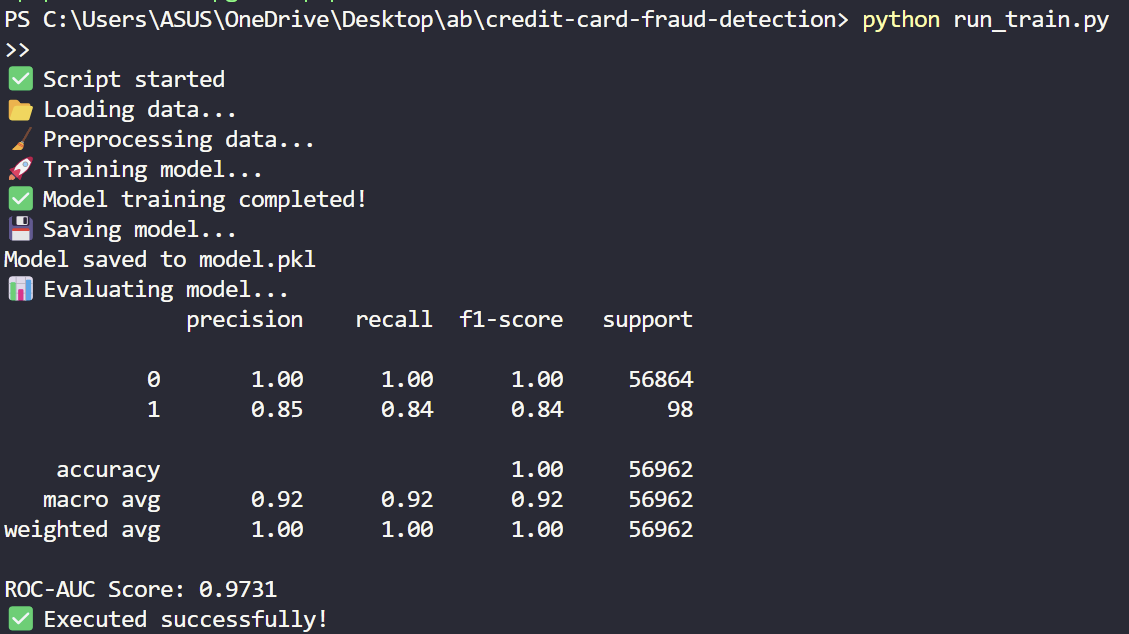
\includegraphics[width=481.95bp,height=270.65bp]{images/image_p47_39.png}};
  \node[anchor=north west,inner sep=0pt,outer sep=0pt] at (500.86,772.91) {{\fontsize{11.0bp}{13.2bp}\selectfont 39 | }};
  \node[anchor=north west,inner sep=0pt,outer sep=0pt] at (519.58,772.91) {{\fontsize{11.0bp}{13.2bp}\selectfont \textcolor{pdfcolor1}{P a g e}}};
  \node[anchor=north west,inner sep=0pt,outer sep=0pt] at (550.14,772.91) {{\fontsize{11.0bp}{13.2bp}\selectfont   }};
  \node[anchor=north west,inner sep=0pt,outer sep=0pt] at (271.80,83.31) {{\fontsize{16.1bp}{19.3bp}\selectfont \textbf{6. RESULT }}};
  \node[anchor=north west,inner sep=0pt,outer sep=0pt] at (159.91,121.02) {{\fontsize{16.1bp}{19.3bp}\selectfont \textbf{6.1 Experimental Result 1 (Model Accuracy) }}};
  \node[anchor=north west,inner sep=0pt,outer sep=0pt] at (70.82,479.98) {{\fontsize{12.0bp}{14.4bp}\selectfont The training script run\_train.py was executed to train and evaluate the Random Forest Classifier on }};
  \node[anchor=north west,inner sep=0pt,outer sep=0pt] at (70.82,495.82) {{\fontsize{12.0bp}{14.4bp}\selectfont the credit card fraud detection dataset. The pipeline includes preprocessing, SMOTE-based }};
  \node[anchor=north west,inner sep=0pt,outer sep=0pt] at (70.82,511.66) {{\fontsize{12.0bp}{14.4bp}\selectfont resampling, model training, and evaluation. Below is a screenshot of the terminal output: }};
  \node[anchor=north west,inner sep=0pt,outer sep=0pt] at (70.82,537.69) {{\fontsize{12.0bp}{14.4bp}\selectfont \textbf{Evaluation Metrics:}}};
  \node[anchor=north west,inner sep=0pt,outer sep=0pt] at (173.11,537.58) {{\fontsize{12.0bp}{14.4bp}\selectfont  }};
  \node[anchor=north west,inner sep=0pt,outer sep=0pt] at (88.85,566.04) {{\fontsize{10.1bp}{12.1bp}\selectfont •}};
  \node[anchor=north west,inner sep=0pt,outer sep=0pt] at (93.41,565.33) {\textsf{{\fontsize{10.1bp}{12.1bp}\selectfont  }}};
  \node[anchor=north west,inner sep=0pt,outer sep=0pt] at (106.85,563.64) {{\fontsize{12.0bp}{14.4bp}\selectfont \textbf{Accuracy}}};
  \node[anchor=north west,inner sep=0pt,outer sep=0pt] at (155.35,563.53) {{\fontsize{12.0bp}{14.4bp}\selectfont : 100\% }};
  \node[anchor=north west,inner sep=0pt,outer sep=0pt] at (88.85,591.96) {{\fontsize{10.1bp}{12.1bp}\selectfont •}};
  \node[anchor=north west,inner sep=0pt,outer sep=0pt] at (93.41,591.25) {\textsf{{\fontsize{10.1bp}{12.1bp}\selectfont  }}};
  \node[anchor=north west,inner sep=0pt,outer sep=0pt] at (106.85,589.56) {{\fontsize{12.0bp}{14.4bp}\selectfont \textbf{Precision (Fraud Class - 1)}}};
  \node[anchor=north west,inner sep=0pt,outer sep=0pt] at (243.70,589.45) {{\fontsize{12.0bp}{14.4bp}\selectfont : 0.85 }};
  \node[anchor=north west,inner sep=0pt,outer sep=0pt] at (88.85,617.88) {{\fontsize{10.1bp}{12.1bp}\selectfont •}};
  \node[anchor=north west,inner sep=0pt,outer sep=0pt] at (93.41,617.17) {\textsf{{\fontsize{10.1bp}{12.1bp}\selectfont  }}};
  \node[anchor=north west,inner sep=0pt,outer sep=0pt] at (106.85,615.48) {{\fontsize{12.0bp}{14.4bp}\selectfont \textbf{Recall (Fraud Class - 1)}}};
  \node[anchor=north west,inner sep=0pt,outer sep=0pt] at (228.34,615.37) {{\fontsize{12.0bp}{14.4bp}\selectfont : 0.84 }};
  \node[anchor=north west,inner sep=0pt,outer sep=0pt] at (88.85,643.58) {{\fontsize{10.1bp}{12.1bp}\selectfont •}};
  \node[anchor=north west,inner sep=0pt,outer sep=0pt] at (93.41,642.87) {\textsf{{\fontsize{10.1bp}{12.1bp}\selectfont  }}};
  \node[anchor=north west,inner sep=0pt,outer sep=0pt] at (106.85,641.18) {{\fontsize{12.0bp}{14.4bp}\selectfont \textbf{F1 Score (Fraud Class - 1)}}};
  \node[anchor=north west,inner sep=0pt,outer sep=0pt] at (241.30,641.07) {{\fontsize{12.0bp}{14.4bp}\selectfont : 0.84 }};
  \node[anchor=north west,inner sep=0pt,outer sep=0pt] at (88.85,669.50) {{\fontsize{10.1bp}{12.1bp}\selectfont •}};
  \node[anchor=north west,inner sep=0pt,outer sep=0pt] at (93.41,668.79) {\textsf{{\fontsize{10.1bp}{12.1bp}\selectfont  }}};
  \node[anchor=north west,inner sep=0pt,outer sep=0pt] at (106.85,667.10) {{\fontsize{12.0bp}{14.4bp}\selectfont \textbf{ROC-AUC Score}}};
  \node[anchor=north west,inner sep=0pt,outer sep=0pt] at (195.19,666.99) {{\fontsize{12.0bp}{14.4bp}\selectfont : 0.9731 }};
  \node[anchor=north west,inner sep=0pt,outer sep=0pt] at (70.82,692.91) {{\fontsize{12.0bp}{14.4bp}\selectfont These results indicate a robust and high-performing model capable of distinguishing between }};
  \node[anchor=north west,inner sep=0pt,outer sep=0pt] at (70.82,708.75) {{\fontsize{12.0bp}{14.4bp}\selectfont fraudulent and legitimate transactions effectively. The model was saved as model.pkl and is used }};
  \node[anchor=north west,inner sep=0pt,outer sep=0pt] at (70.82,724.62) {{\fontsize{12.0bp}{14.4bp}\selectfont for real-time predictions via the Streamlit interface. }};
\end{tikzpicture}
\newpage
\noindent
\begin{tikzpicture}[x=1bp,y=-1bp,inner sep=0pt,outer sep=0pt]
  \useasboundingbox (0,0) rectangle (595.20,841.92);
  \fill[fill=pdfcolor9] (69.38,772.78) rectangle (554.40,773.26);
  \fill[fill=black] (146.23,101.78) rectangle (477.31,103.22);
  \node[anchor=north west,inner sep=0pt] at (70.90,153.81) {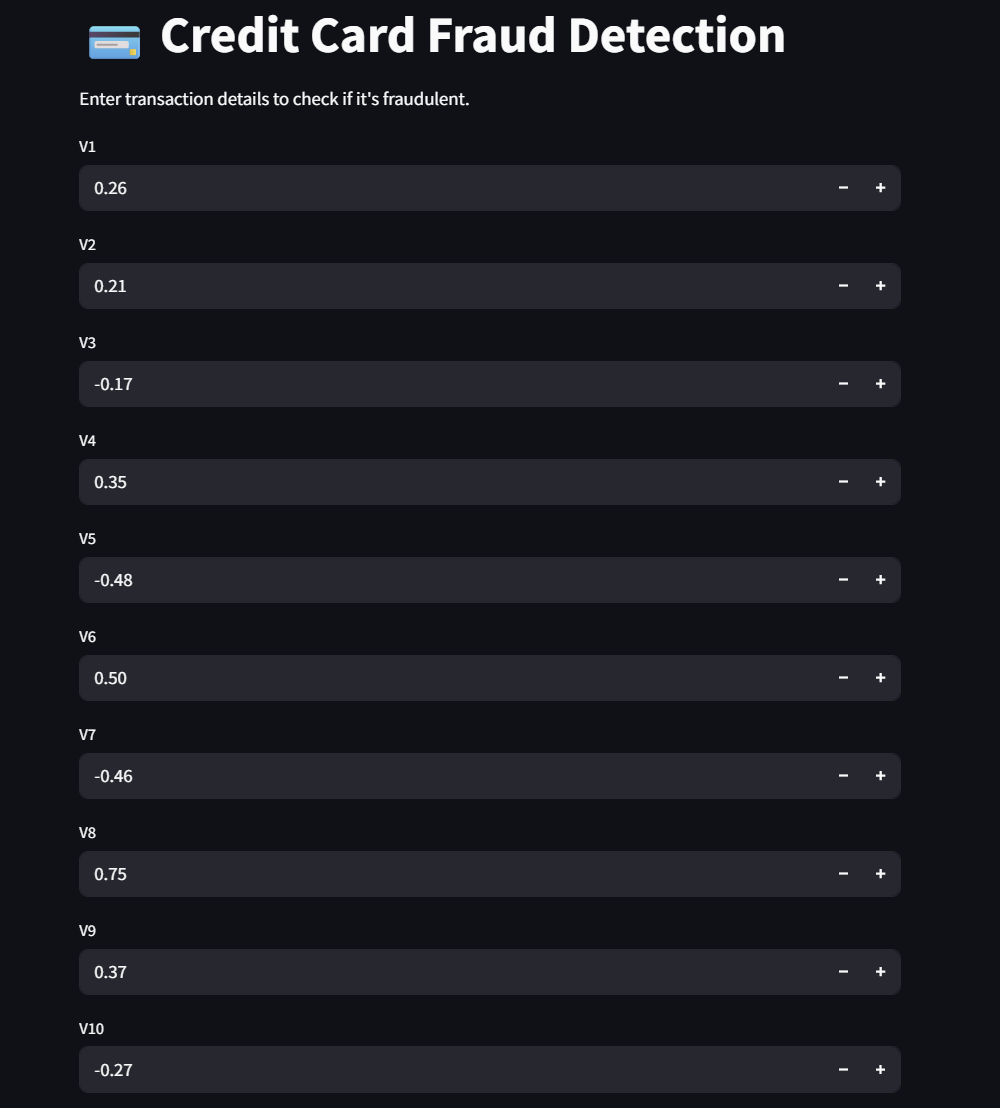
\includegraphics[width=481.95bp,height=534.00bp]{images/image_p48_40.png}};
  \node[anchor=north west,inner sep=0pt,outer sep=0pt] at (500.86,772.91) {{\fontsize{11.0bp}{13.2bp}\selectfont 40 | }};
  \node[anchor=north west,inner sep=0pt,outer sep=0pt] at (519.58,772.91) {{\fontsize{11.0bp}{13.2bp}\selectfont \textcolor{pdfcolor1}{P a g e}}};
  \node[anchor=north west,inner sep=0pt,outer sep=0pt] at (550.14,772.91) {{\fontsize{11.0bp}{13.2bp}\selectfont   }};
  \node[anchor=north west,inner sep=0pt,outer sep=0pt] at (146.23,83.31) {{\fontsize{16.1bp}{19.3bp}\selectfont \textbf{6.2 Experimental Result 2 (Streamlit UI Output) }}};
\end{tikzpicture}
\newpage
\noindent
\begin{tikzpicture}[x=1bp,y=-1bp,inner sep=0pt,outer sep=0pt]
  \useasboundingbox (0,0) rectangle (595.20,841.92);
  \fill[fill=pdfcolor9] (69.38,772.78) rectangle (554.40,773.26);
  \node[anchor=north west,inner sep=0pt] at (70.90,85.05) {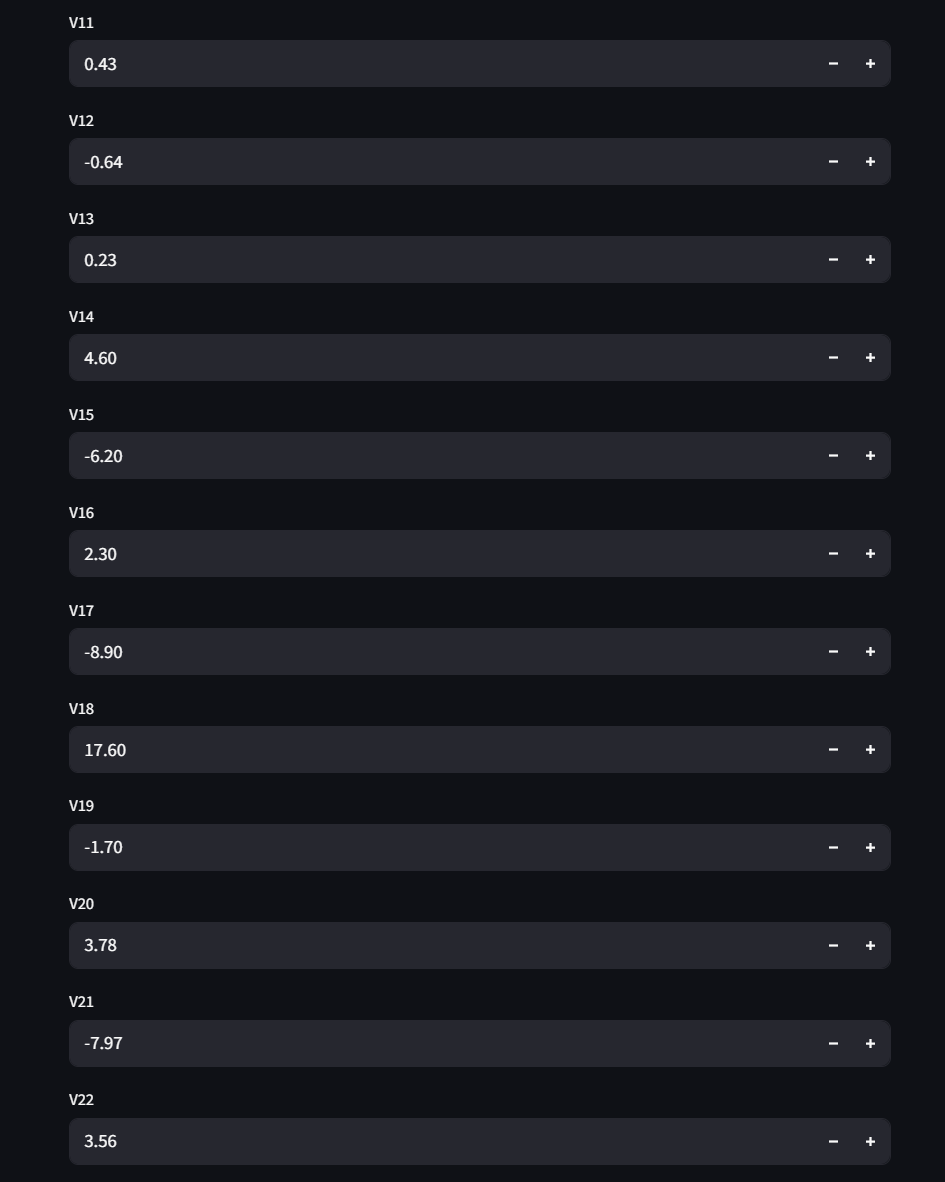
\includegraphics[width=481.95bp,height=602.85bp]{images/image_p49_41.png}};
  \node[anchor=north west,inner sep=0pt,outer sep=0pt] at (500.86,772.91) {{\fontsize{11.0bp}{13.2bp}\selectfont 41 | }};
  \node[anchor=north west,inner sep=0pt,outer sep=0pt] at (519.58,772.91) {{\fontsize{11.0bp}{13.2bp}\selectfont \textcolor{pdfcolor1}{P a g e}}};
  \node[anchor=north west,inner sep=0pt,outer sep=0pt] at (550.14,772.91) {{\fontsize{11.0bp}{13.2bp}\selectfont   }};
\end{tikzpicture}
\newpage
\noindent
\begin{tikzpicture}[x=1bp,y=-1bp,inner sep=0pt,outer sep=0pt]
  \useasboundingbox (0,0) rectangle (595.20,841.92);
  \fill[fill=pdfcolor9] (69.38,772.78) rectangle (554.40,773.26);
  \node[anchor=north west,inner sep=0pt] at (70.90,85.05) {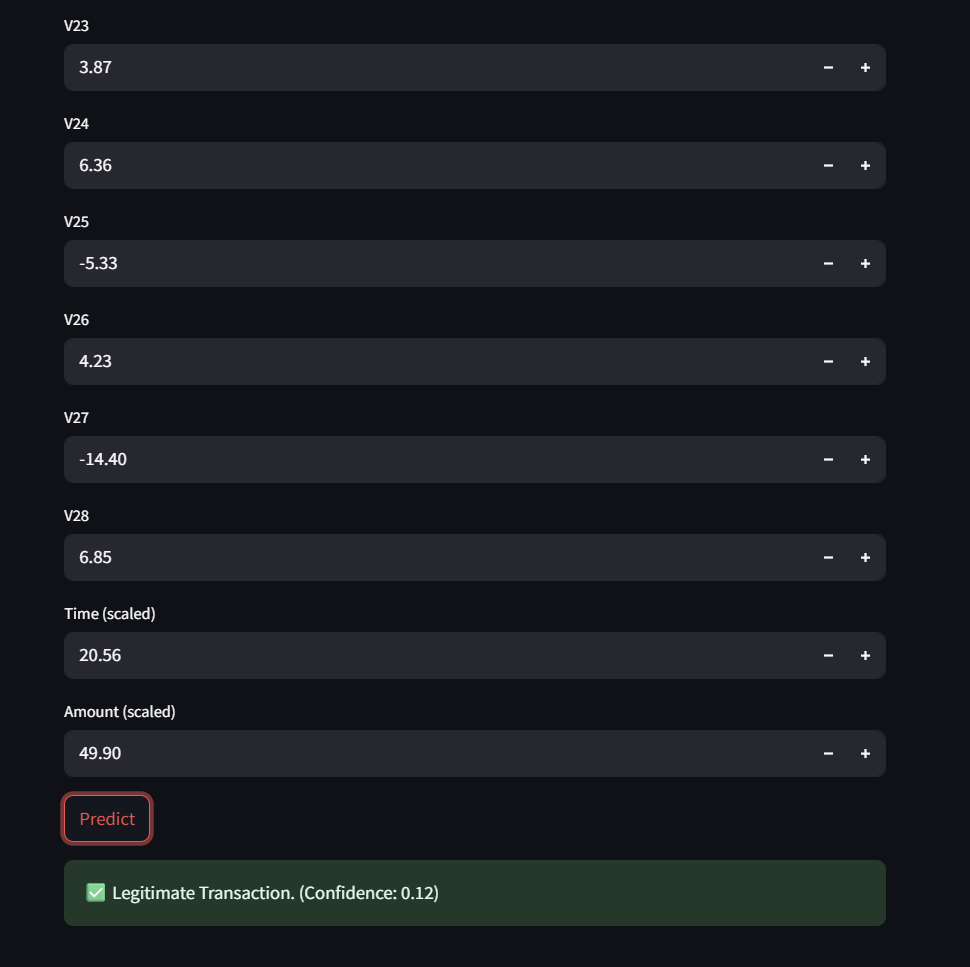
\includegraphics[width=481.95bp,height=480.45bp]{images/image_p50_42.png}};
  \node[anchor=north west,inner sep=0pt,outer sep=0pt] at (500.86,772.91) {{\fontsize{11.0bp}{13.2bp}\selectfont 42 | }};
  \node[anchor=north west,inner sep=0pt,outer sep=0pt] at (519.58,772.91) {{\fontsize{11.0bp}{13.2bp}\selectfont \textcolor{pdfcolor1}{P a g e}}};
  \node[anchor=north west,inner sep=0pt,outer sep=0pt] at (550.14,772.91) {{\fontsize{11.0bp}{13.2bp}\selectfont   }};
\end{tikzpicture}
\newpage
\noindent
\begin{tikzpicture}[x=1bp,y=-1bp,inner sep=0pt,outer sep=0pt]
  \useasboundingbox (0,0) rectangle (595.20,841.92);
  \fill[fill=pdfcolor9] (69.38,772.78) rectangle (554.40,773.26);
  \fill[fill=black] (142.87,101.78) rectangle (456.91,103.22);
  \fill[fill=black] (178.87,560.81) rectangle (448.75,562.25);
  \node[anchor=north west,inner sep=0pt] at (70.90,147.37) {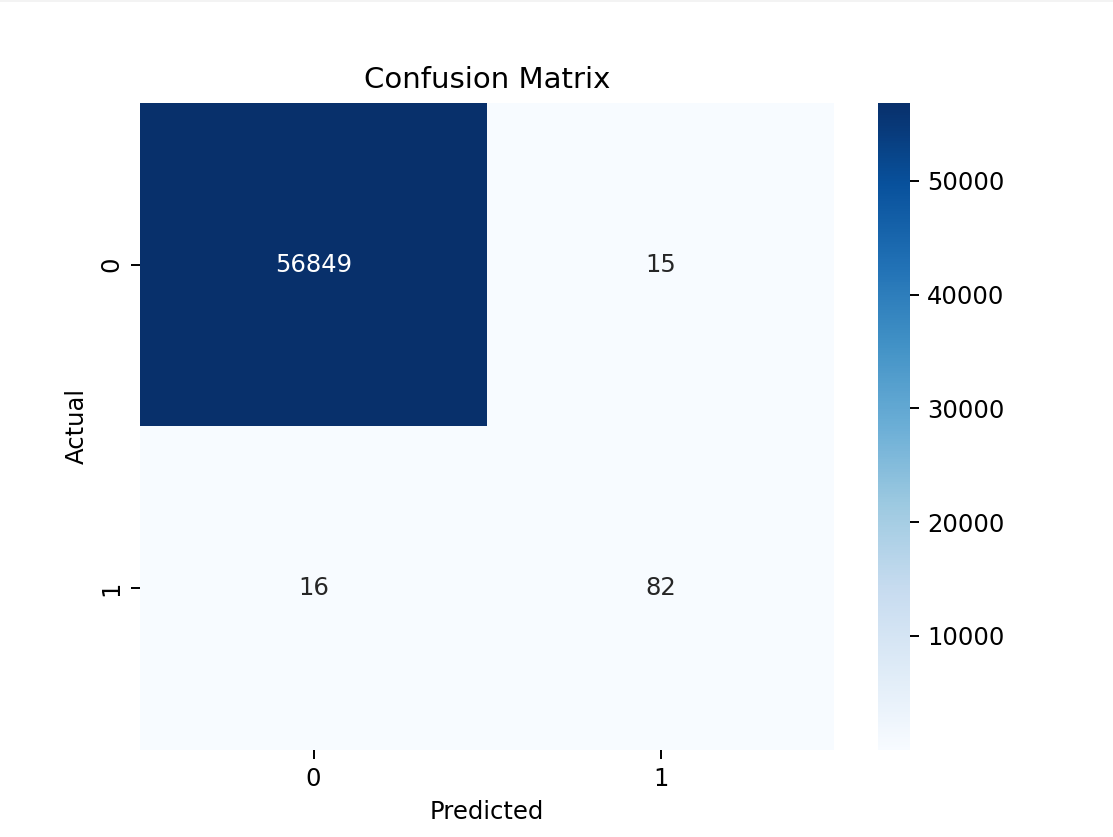
\includegraphics[width=468.85bp,height=352.55bp]{images/image_p51_43.png}};
  \node[anchor=north west,inner sep=0pt] at (70.90,606.15) {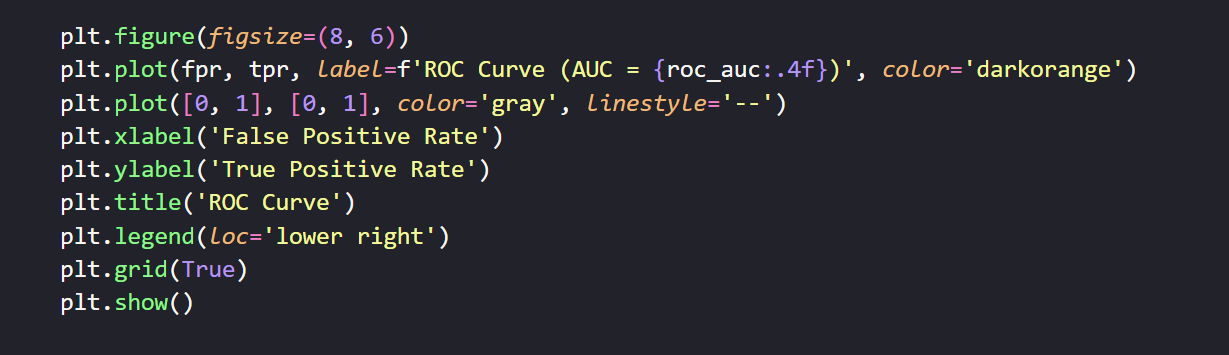
\includegraphics[width=468.00bp,height=135.15bp]{images/image_p51_44.png}};
  \node[anchor=north west,inner sep=0pt,outer sep=0pt] at (500.86,772.91) {{\fontsize{11.0bp}{13.2bp}\selectfont 43 | }};
  \node[anchor=north west,inner sep=0pt,outer sep=0pt] at (519.58,772.91) {{\fontsize{11.0bp}{13.2bp}\selectfont \textcolor{pdfcolor1}{P a g e}}};
  \node[anchor=north west,inner sep=0pt,outer sep=0pt] at (550.14,772.91) {{\fontsize{11.0bp}{13.2bp}\selectfont   }};
  \node[anchor=north west,inner sep=0pt,outer sep=0pt] at (142.87,83.31) {{\fontsize{16.1bp}{19.3bp}\selectfont \textbf{6.3 Experimental Result 3 (Confusion Matrix)  }}};
  \node[anchor=north west,inner sep=0pt,outer sep=0pt] at (178.87,542.34) {{\fontsize{16.1bp}{19.3bp}\selectfont \textbf{6.4 Experimental Result 4(ROC Curve)}}};
  \node[anchor=north west,inner sep=0pt,outer sep=0pt] at (448.75,542.20) {{\fontsize{16.1bp}{19.3bp}\selectfont  }};
\end{tikzpicture}
\newpage
\noindent
\begin{tikzpicture}[x=1bp,y=-1bp,inner sep=0pt,outer sep=0pt]
  \useasboundingbox (0,0) rectangle (595.20,841.92);
  \fill[fill=pdfcolor9] (69.38,772.78) rectangle (554.40,773.26);
  \node[anchor=north west,inner sep=0pt] at (70.90,85.05) {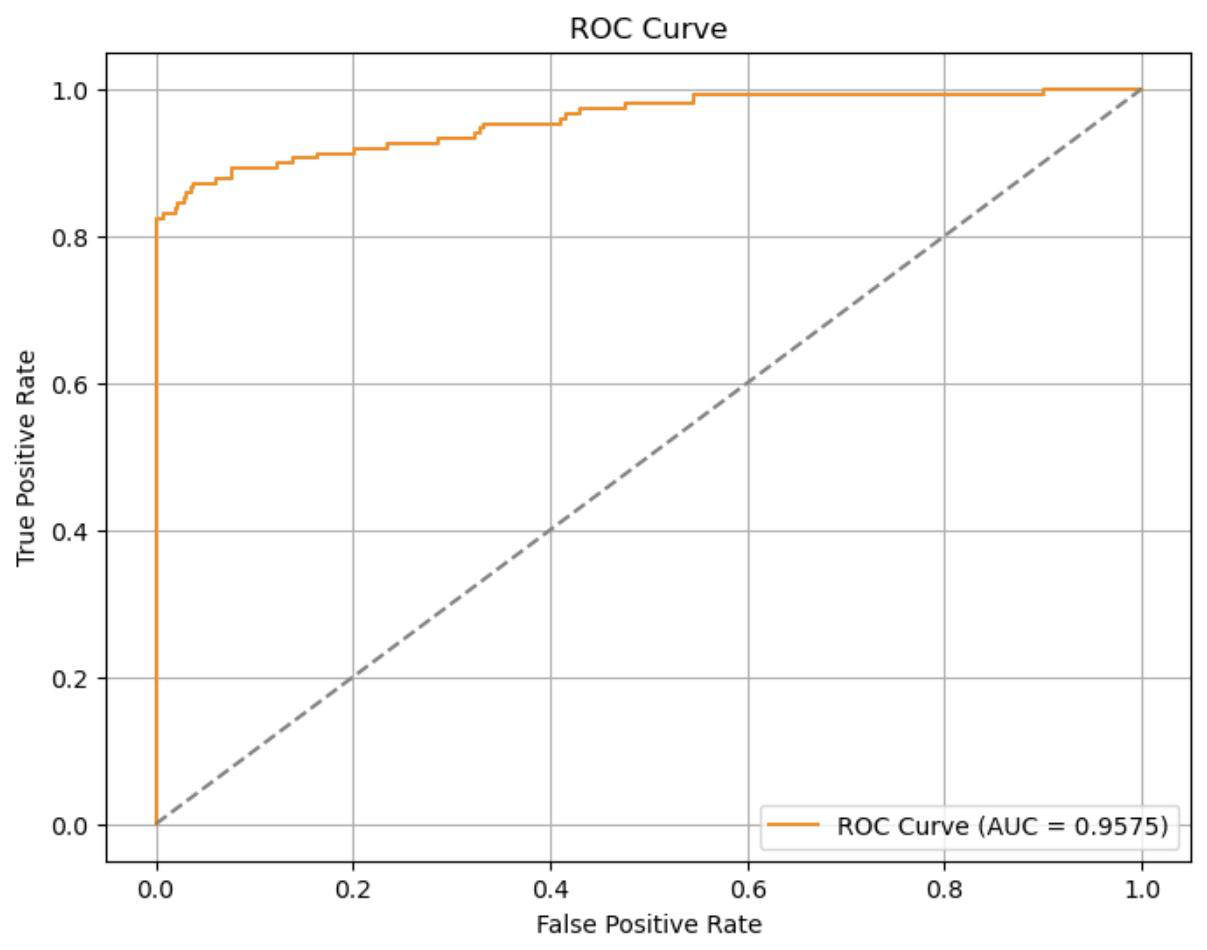
\includegraphics[width=468.00bp,height=368.35bp]{images/image_p52_45.png}};
  \node[anchor=north west,inner sep=0pt,outer sep=0pt] at (500.86,772.91) {{\fontsize{11.0bp}{13.2bp}\selectfont 44 | }};
  \node[anchor=north west,inner sep=0pt,outer sep=0pt] at (519.58,772.91) {{\fontsize{11.0bp}{13.2bp}\selectfont \textcolor{pdfcolor1}{P a g e}}};
  \node[anchor=north west,inner sep=0pt,outer sep=0pt] at (550.14,772.91) {{\fontsize{11.0bp}{13.2bp}\selectfont   }};
\end{tikzpicture}
\newpage
\noindent
\begin{tikzpicture}[x=1bp,y=-1bp,inner sep=0pt,outer sep=0pt]
  \useasboundingbox (0,0) rectangle (595.20,841.92);
  \fill[fill=pdfcolor9] (69.38,772.78) rectangle (554.40,773.26);
  \fill[fill=black] (249.46,101.78) rectangle (374.09,103.22);
  \node[anchor=north west,inner sep=0pt,outer sep=0pt] at (500.86,772.91) {{\fontsize{11.0bp}{13.2bp}\selectfont 45 | }};
  \node[anchor=north west,inner sep=0pt,outer sep=0pt] at (519.58,772.91) {{\fontsize{11.0bp}{13.2bp}\selectfont \textcolor{pdfcolor1}{P a g e}}};
  \node[anchor=north west,inner sep=0pt,outer sep=0pt] at (550.14,772.91) {{\fontsize{11.0bp}{13.2bp}\selectfont   }};
  \node[anchor=north west,inner sep=0pt,outer sep=0pt] at (249.46,83.31) {{\fontsize{16.1bp}{19.3bp}\selectfont \textbf{7. CONCLUSION }}};
  \node[anchor=north west,inner sep=0pt,outer sep=0pt] at (70.82,121.33) {{\fontsize{12.0bp}{14.4bp}\selectfont The Credit Card Fraud Detection System developed in this project offers a robust, scalable, and }};
  \node[anchor=north west,inner sep=0pt,outer sep=0pt] at (70.82,141.97) {{\fontsize{12.0bp}{14.4bp}\selectfont user-friendly solution to one of the most pressing issues in the digital economy: fraudulent }};
  \node[anchor=north west,inner sep=0pt,outer sep=0pt] at (70.82,162.85) {{\fontsize{12.0bp}{14.4bp}\selectfont transactions. Leveraging machine learning, particularly supervised classification through Random }};
  \node[anchor=north west,inner sep=0pt,outer sep=0pt] at (70.82,183.49) {{\fontsize{12.0bp}{14.4bp}\selectfont Forest, the system effectively differentiates between legitimate and fraudulent credit card }};
  \node[anchor=north west,inner sep=0pt,outer sep=0pt] at (70.82,204.15) {{\fontsize{12.0bp}{14.4bp}\selectfont transactions based on historical patterns. By integrating advanced techniques such as Synthetic }};
  \node[anchor=north west,inner sep=0pt,outer sep=0pt] at (70.82,224.79) {{\fontsize{12.0bp}{14.4bp}\selectfont Minority Over-sampling Technique (SMOTE), the project addresses the critical issue of class }};
  \node[anchor=north west,inner sep=0pt,outer sep=0pt] at (70.82,245.43) {{\fontsize{12.0bp}{14.4bp}\selectfont imbalance, a common challenge in fraud detection scenarios. }};
  \node[anchor=north west,inner sep=0pt,outer sep=0pt] at (70.82,276.15) {{\fontsize{12.0bp}{14.4bp}\selectfont From the early stages of data preprocessing---where Time and Amount are normalized and }};
  \node[anchor=north west,inner sep=0pt,outer sep=0pt] at (70.82,297.06) {{\fontsize{12.0bp}{14.4bp}\selectfont anonymized features (V1 to V28) are utilized---to model training and evaluation, the system }};
  \node[anchor=north west,inner sep=0pt,outer sep=0pt] at (70.82,317.70) {{\fontsize{12.0bp}{14.4bp}\selectfont demonstrates end-to-end competency. The use of ROC-AUC, Precision, Recall, and F1-score }};
  \node[anchor=north west,inner sep=0pt,outer sep=0pt] at (70.82,338.34) {{\fontsize{12.0bp}{14.4bp}\selectfont ensures that model performance is measured not only by overall accuracy but also by how well it }};
  \node[anchor=north west,inner sep=0pt,outer sep=0pt] at (70.82,358.98) {{\fontsize{12.0bp}{14.4bp}\selectfont handles rare but impactful fraud cases. This evaluation strategy enhances the model's reliability and }};
  \node[anchor=north west,inner sep=0pt,outer sep=0pt] at (70.82,379.88) {{\fontsize{12.0bp}{14.4bp}\selectfont trustworthiness in real-world applications. }};
  \node[anchor=north west,inner sep=0pt,outer sep=0pt] at (70.82,410.60) {{\fontsize{12.0bp}{14.4bp}\selectfont The deployment of the trained model via Streamlit introduces a practical and accessible interface, }};
  \node[anchor=north west,inner sep=0pt,outer sep=0pt] at (70.82,431.24) {{\fontsize{12.0bp}{14.4bp}\selectfont transforming the theoretical model into a user-operable system. Users can enter transaction details }};
  \node[anchor=north west,inner sep=0pt,outer sep=0pt] at (70.82,451.88) {{\fontsize{12.0bp}{14.4bp}\selectfont and instantly receive a prediction, making this tool suitable for integration into customer service }};
  \node[anchor=north west,inner sep=0pt,outer sep=0pt] at (70.82,472.54) {{\fontsize{12.0bp}{14.4bp}\selectfont desks, financial institutions, and digital wallets. The system's architecture is modular, with each }};
  \node[anchor=north west,inner sep=0pt,outer sep=0pt] at (70.82,493.18) {{\fontsize{12.0bp}{14.4bp}\selectfont part---from data preprocessing and training to evaluation and prediction---being independently }};
  \node[anchor=north west,inner sep=0pt,outer sep=0pt] at (70.82,514.06) {{\fontsize{12.0bp}{14.4bp}\selectfont testable and extensible. }};
  \node[anchor=north west,inner sep=0pt,outer sep=0pt] at (70.82,544.81) {{\fontsize{12.0bp}{14.4bp}\selectfont A significant contribution of this project is its educational value. It not only demonstrates how to }};
  \node[anchor=north west,inner sep=0pt,outer sep=0pt] at (70.82,565.45) {{\fontsize{12.0bp}{14.4bp}\selectfont build a data-driven, intelligent fraud detection system but also serves as a comprehensive case study }};
  \node[anchor=north west,inner sep=0pt,outer sep=0pt] at (70.82,586.09) {{\fontsize{12.0bp}{14.4bp}\selectfont in solving real-world problems using AI and machine learning. Students and practitioners can build }};
  \node[anchor=north west,inner sep=0pt,outer sep=0pt] at (70.82,606.73) {{\fontsize{12.0bp}{14.4bp}\selectfont upon this framework to experiment with alternative algorithms, incorporate real-time streaming }};
  \node[anchor=north west,inner sep=0pt,outer sep=0pt] at (70.82,627.61) {{\fontsize{12.0bp}{14.4bp}\selectfont data, or expand the dataset with additional transaction metadata. }};
  \node[anchor=north west,inner sep=0pt,outer sep=0pt] at (70.82,658.35) {{\fontsize{12.0bp}{14.4bp}\selectfont Moreover, the system's documentation, modularity, and adherence to best practices such as code }};
  \node[anchor=north west,inner sep=0pt,outer sep=0pt] at (70.82,678.99) {{\fontsize{12.0bp}{14.4bp}\selectfont reusability and environment isolation through virtual environments make it easy to deploy and }};
  \node[anchor=north west,inner sep=0pt,outer sep=0pt] at (70.82,699.63) {{\fontsize{12.0bp}{14.4bp}\selectfont maintain. The use of open-source libraries and publicly available datasets reinforces the project’s }};
  \node[anchor=north west,inner sep=0pt,outer sep=0pt] at (70.82,720.30) {{\fontsize{12.0bp}{14.4bp}\selectfont reproducibility and accessibility. }};
\end{tikzpicture}
\newpage
\noindent
\begin{tikzpicture}[x=1bp,y=-1bp,inner sep=0pt,outer sep=0pt]
  \useasboundingbox (0,0) rectangle (595.20,841.92);
  \fill[fill=pdfcolor9] (69.38,772.78) rectangle (554.40,773.26);
  \node[anchor=north west,inner sep=0pt,outer sep=0pt] at (500.86,772.91) {{\fontsize{11.0bp}{13.2bp}\selectfont 46 | }};
  \node[anchor=north west,inner sep=0pt,outer sep=0pt] at (519.58,772.91) {{\fontsize{11.0bp}{13.2bp}\selectfont \textcolor{pdfcolor1}{P a g e}}};
  \node[anchor=north west,inner sep=0pt,outer sep=0pt] at (550.14,772.91) {{\fontsize{11.0bp}{13.2bp}\selectfont   }};
  \node[anchor=north west,inner sep=0pt,outer sep=0pt] at (70.82,83.62) {{\fontsize{12.0bp}{14.4bp}\selectfont Despite its effectiveness, the system is not without limitations. It relies on static, historical data and }};
  \node[anchor=north west,inner sep=0pt,outer sep=0pt] at (70.82,104.50) {{\fontsize{12.0bp}{14.4bp}\selectfont does not incorporate temporal patterns or real-time anomaly detection. Future improvements could }};
  \node[anchor=north west,inner sep=0pt,outer sep=0pt] at (70.82,125.17) {{\fontsize{12.0bp}{14.4bp}\selectfont include integrating deep learning models such as LSTM for sequential behavior analysis or }};
  \node[anchor=north west,inner sep=0pt,outer sep=0pt] at (70.82,145.81) {{\fontsize{12.0bp}{14.4bp}\selectfont implementing unsupervised anomaly detection methods to capture novel fraud patterns. }};
  \node[anchor=north west,inner sep=0pt,outer sep=0pt] at (70.82,176.53) {{\fontsize{12.0bp}{14.4bp}\selectfont In conclusion, this project successfully meets its stated objectives by designing and deploying a }};
  \node[anchor=north west,inner sep=0pt,outer sep=0pt] at (70.82,197.17) {{\fontsize{12.0bp}{14.4bp}\selectfont credit card fraud detection system that is both technically sound and practically usable. It }};
  \node[anchor=north west,inner sep=0pt,outer sep=0pt] at (70.82,217.83) {{\fontsize{12.0bp}{14.4bp}\selectfont contributes to the broader field of financial technology by offering a model that balances }};
  \node[anchor=north west,inner sep=0pt,outer sep=0pt] at (70.82,238.71) {{\fontsize{12.0bp}{14.4bp}\selectfont performance, interpretability, and usability. With further enhancements, the system holds potential }};
  \node[anchor=north west,inner sep=0pt,outer sep=0pt] at (70.82,259.35) {{\fontsize{12.0bp}{14.4bp}\selectfont for adoption in large-scale fraud monitoring environments, paving the way for smarter and more }};
  \node[anchor=north west,inner sep=0pt,outer sep=0pt] at (70.82,279.99) {{\fontsize{12.0bp}{14.4bp}\selectfont secure digital transactions. }};
\end{tikzpicture}
\newpage
\noindent
\begin{tikzpicture}[x=1bp,y=-1bp,inner sep=0pt,outer sep=0pt]
  \useasboundingbox (0,0) rectangle (595.20,841.92);
  \fill[fill=pdfcolor9] (69.38,772.78) rectangle (554.40,773.26);
  \fill[fill=black] (242.26,101.78) rectangle (381.53,103.22);
  \node[anchor=north west,inner sep=0pt,outer sep=0pt] at (500.86,772.91) {{\fontsize{11.0bp}{13.2bp}\selectfont 47 | }};
  \node[anchor=north west,inner sep=0pt,outer sep=0pt] at (519.58,772.91) {{\fontsize{11.0bp}{13.2bp}\selectfont \textcolor{pdfcolor1}{P a g e}}};
  \node[anchor=north west,inner sep=0pt,outer sep=0pt] at (550.14,772.91) {{\fontsize{11.0bp}{13.2bp}\selectfont   }};
  \node[anchor=north west,inner sep=0pt,outer sep=0pt] at (242.26,83.31) {{\fontsize{16.1bp}{19.3bp}\selectfont \textbf{8. FUTURE SCOPE }}};
  \node[anchor=north west,inner sep=0pt,outer sep=0pt] at (70.82,121.33) {{\fontsize{12.0bp}{14.4bp}\selectfont The credit card fraud detection system developed in this project lays a strong foundation for }};
  \node[anchor=north west,inner sep=0pt,outer sep=0pt] at (70.82,137.17) {{\fontsize{12.0bp}{14.4bp}\selectfont combating financial fraud through data science and machine learning. While the current version is }};
  \node[anchor=north west,inner sep=0pt,outer sep=0pt] at (70.82,153.01) {{\fontsize{12.0bp}{14.4bp}\selectfont effective for academic and prototype purposes, there are multiple avenues for extending and }};
  \node[anchor=north west,inner sep=0pt,outer sep=0pt] at (70.82,168.85) {{\fontsize{12.0bp}{14.4bp}\selectfont enhancing the system to meet industry-scale requirements. Below are several key areas where the }};
  \node[anchor=north west,inner sep=0pt,outer sep=0pt] at (70.82,184.93) {{\fontsize{12.0bp}{14.4bp}\selectfont project can evolve: }};
  \node[anchor=north west,inner sep=0pt,outer sep=0pt] at (70.82,210.74) {{\fontsize{12.0bp}{14.4bp}\selectfont \textbf{8.1 Real-Time Fraud Detection }}};
  \node[anchor=north west,inner sep=0pt,outer sep=0pt] at (88.85,239.06) {{\fontsize{10.1bp}{12.1bp}\selectfont •}};
  \node[anchor=north west,inner sep=0pt,outer sep=0pt] at (93.41,238.35) {\textsf{{\fontsize{10.1bp}{12.1bp}\selectfont  }}};
  \node[anchor=north west,inner sep=0pt,outer sep=0pt] at (106.85,236.55) {{\fontsize{12.0bp}{14.4bp}\selectfont Currently, the model processes static datasets. In the future, the system can be integrated }};
  \node[anchor=north west,inner sep=0pt,outer sep=0pt] at (106.85,252.39) {{\fontsize{12.0bp}{14.4bp}\selectfont with real-time streaming data using tools such as Apache Kafka or AWS Kinesis. }};
  \node[anchor=north west,inner sep=0pt,outer sep=0pt] at (88.85,280.82) {{\fontsize{10.1bp}{12.1bp}\selectfont •}};
  \node[anchor=north west,inner sep=0pt,outer sep=0pt] at (93.41,280.11) {\textsf{{\fontsize{10.1bp}{12.1bp}\selectfont  }}};
  \node[anchor=north west,inner sep=0pt,outer sep=0pt] at (106.85,278.31) {{\fontsize{12.0bp}{14.4bp}\selectfont This will enable the detection of frauds as they happen, minimizing potential financial loss. }};
  \node[anchor=north west,inner sep=0pt,outer sep=0pt] at (70.82,304.37) {{\fontsize{12.0bp}{14.4bp}\selectfont \textbf{8.2 Integration with Cloud Services }}};
  \node[anchor=north west,inner sep=0pt,outer sep=0pt] at (88.85,332.69) {{\fontsize{10.1bp}{12.1bp}\selectfont •}};
  \node[anchor=north west,inner sep=0pt,outer sep=0pt] at (93.41,331.98) {\textsf{{\fontsize{10.1bp}{12.1bp}\selectfont  }}};
  \node[anchor=north west,inner sep=0pt,outer sep=0pt] at (106.85,330.18) {{\fontsize{12.0bp}{14.4bp}\selectfont Deploying the model on cloud platforms such as AWS, GCP, or Azure can improve }};
  \node[anchor=north west,inner sep=0pt,outer sep=0pt] at (106.85,346.02) {{\fontsize{12.0bp}{14.4bp}\selectfont scalability and availability. }};
  \node[anchor=north west,inner sep=0pt,outer sep=0pt] at (88.85,374.23) {{\fontsize{10.1bp}{12.1bp}\selectfont •}};
  \node[anchor=north west,inner sep=0pt,outer sep=0pt] at (93.41,373.52) {\textsf{{\fontsize{10.1bp}{12.1bp}\selectfont  }}};
  \node[anchor=north west,inner sep=0pt,outer sep=0pt] at (106.85,371.72) {{\fontsize{12.0bp}{14.4bp}\selectfont Integration with cloud databases and monitoring tools can support millions of transactions }};
  \node[anchor=north west,inner sep=0pt,outer sep=0pt] at (106.85,387.80) {{\fontsize{12.0bp}{14.4bp}\selectfont per day with ease. }};
  \node[anchor=north west,inner sep=0pt,outer sep=0pt] at (70.82,413.59) {{\fontsize{12.0bp}{14.4bp}\selectfont \textbf{8.3 Advanced Deep Learning Models }}};
  \node[anchor=north west,inner sep=0pt,outer sep=0pt] at (88.85,441.91) {{\fontsize{10.1bp}{12.1bp}\selectfont •}};
  \node[anchor=north west,inner sep=0pt,outer sep=0pt] at (93.41,441.20) {\textsf{{\fontsize{10.1bp}{12.1bp}\selectfont  }}};
  \node[anchor=north west,inner sep=0pt,outer sep=0pt] at (106.85,439.40) {{\fontsize{12.0bp}{14.4bp}\selectfont Deep learning architectures like LSTM and GRU can be introduced to learn temporal }};
  \node[anchor=north west,inner sep=0pt,outer sep=0pt] at (106.85,455.24) {{\fontsize{12.0bp}{14.4bp}\selectfont patterns and user behavior over time. }};
  \node[anchor=north west,inner sep=0pt,outer sep=0pt] at (88.85,483.69) {{\fontsize{10.1bp}{12.1bp}\selectfont •}};
  \node[anchor=north west,inner sep=0pt,outer sep=0pt] at (93.41,482.98) {\textsf{{\fontsize{10.1bp}{12.1bp}\selectfont  }}};
  \node[anchor=north west,inner sep=0pt,outer sep=0pt] at (106.85,481.18) {{\fontsize{12.0bp}{14.4bp}\selectfont These models can enhance accuracy and adapt to evolving fraud tactics. }};
  \node[anchor=north west,inner sep=0pt,outer sep=0pt] at (70.82,507.21) {{\fontsize{12.0bp}{14.4bp}\selectfont \textbf{8.4 Model Interpretability and Explainability }}};
  \node[anchor=north west,inner sep=0pt,outer sep=0pt] at (88.85,535.53) {{\fontsize{10.1bp}{12.1bp}\selectfont •}};
  \node[anchor=north west,inner sep=0pt,outer sep=0pt] at (93.41,534.82) {\textsf{{\fontsize{10.1bp}{12.1bp}\selectfont  }}};
  \node[anchor=north west,inner sep=0pt,outer sep=0pt] at (106.85,533.02) {{\fontsize{12.0bp}{14.4bp}\selectfont Adding interpretability tools like SHAP or LIME will allow financial institutions to }};
  \node[anchor=north west,inner sep=0pt,outer sep=0pt] at (106.85,548.89) {{\fontsize{12.0bp}{14.4bp}\selectfont understand why a transaction was marked fraudulent. }};
  \node[anchor=north west,inner sep=0pt,outer sep=0pt] at (88.85,577.32) {{\fontsize{10.1bp}{12.1bp}\selectfont •}};
  \node[anchor=north west,inner sep=0pt,outer sep=0pt] at (93.41,576.61) {\textsf{{\fontsize{10.1bp}{12.1bp}\selectfont  }}};
  \node[anchor=north west,inner sep=0pt,outer sep=0pt] at (106.85,574.81) {{\fontsize{12.0bp}{14.4bp}\selectfont This can build trust and provide valuable insights for auditing and compliance. }};
  \node[anchor=north west,inner sep=0pt,outer sep=0pt] at (70.82,600.60) {{\fontsize{12.0bp}{14.4bp}\selectfont \textbf{8.5 Adaptive Learning }}};
  \node[anchor=north west,inner sep=0pt,outer sep=0pt] at (88.85,628.92) {{\fontsize{10.1bp}{12.1bp}\selectfont •}};
  \node[anchor=north west,inner sep=0pt,outer sep=0pt] at (93.41,628.21) {\textsf{{\fontsize{10.1bp}{12.1bp}\selectfont  }}};
  \node[anchor=north west,inner sep=0pt,outer sep=0pt] at (106.85,626.41) {{\fontsize{12.0bp}{14.4bp}\selectfont Future systems can implement online learning or reinforcement learning models that adapt }};
  \node[anchor=north west,inner sep=0pt,outer sep=0pt] at (106.85,642.27) {{\fontsize{12.0bp}{14.4bp}\selectfont as new data is received. }};
  \node[anchor=north west,inner sep=0pt,outer sep=0pt] at (88.85,670.70) {{\fontsize{10.1bp}{12.1bp}\selectfont •}};
  \node[anchor=north west,inner sep=0pt,outer sep=0pt] at (93.41,669.99) {\textsf{{\fontsize{10.1bp}{12.1bp}\selectfont  }}};
  \node[anchor=north west,inner sep=0pt,outer sep=0pt] at (106.85,668.19) {{\fontsize{12.0bp}{14.4bp}\selectfont This will keep the model up to date without complete retraining, improving performance }};
  \node[anchor=north west,inner sep=0pt,outer sep=0pt] at (106.85,684.03) {{\fontsize{12.0bp}{14.4bp}\selectfont against evolving threats. }};
  \node[anchor=north west,inner sep=0pt,outer sep=0pt] at (70.82,710.06) {{\fontsize{12.0bp}{14.4bp}\selectfont \textbf{8.6 Cross-Domain Applications }}};
  \node[anchor=north west,inner sep=0pt,outer sep=0pt] at (88.85,738.40) {{\fontsize{10.1bp}{12.1bp}\selectfont •}};
  \node[anchor=north west,inner sep=0pt,outer sep=0pt] at (93.41,737.70) {\textsf{{\fontsize{10.1bp}{12.1bp}\selectfont  }}};
  \node[anchor=north west,inner sep=0pt,outer sep=0pt] at (106.85,735.90) {{\fontsize{12.0bp}{14.4bp}\selectfont The same architecture and logic can be adapted for fraud detection in other domains like }};
  \node[anchor=north west,inner sep=0pt,outer sep=0pt] at (106.85,751.74) {{\fontsize{12.0bp}{14.4bp}\selectfont insurance claims, telecom billing, or e-commerce refunds. }};
\end{tikzpicture}
\newpage
\noindent
\begin{tikzpicture}[x=1bp,y=-1bp,inner sep=0pt,outer sep=0pt]
  \useasboundingbox (0,0) rectangle (595.20,841.92);
  \fill[fill=pdfcolor9] (69.38,772.78) rectangle (554.40,773.26);
  \node[anchor=north west,inner sep=0pt,outer sep=0pt] at (500.86,772.91) {{\fontsize{11.0bp}{13.2bp}\selectfont 48 | }};
  \node[anchor=north west,inner sep=0pt,outer sep=0pt] at (519.58,772.91) {{\fontsize{11.0bp}{13.2bp}\selectfont \textcolor{pdfcolor1}{P a g e}}};
  \node[anchor=north west,inner sep=0pt,outer sep=0pt] at (550.14,772.91) {{\fontsize{11.0bp}{13.2bp}\selectfont   }};
  \node[anchor=north west,inner sep=0pt,outer sep=0pt] at (88.85,86.13) {{\fontsize{10.1bp}{12.1bp}\selectfont •}};
  \node[anchor=north west,inner sep=0pt,outer sep=0pt] at (93.41,85.42) {\textsf{{\fontsize{10.1bp}{12.1bp}\selectfont  }}};
  \node[anchor=north west,inner sep=0pt,outer sep=0pt] at (106.85,83.62) {{\fontsize{12.0bp}{14.4bp}\selectfont With minor modifications in the dataset and features, the model can be repurposed }};
  \node[anchor=north west,inner sep=0pt,outer sep=0pt] at (106.85,99.46) {{\fontsize{12.0bp}{14.4bp}\selectfont effectively. }};
  \node[anchor=north west,inner sep=0pt,outer sep=0pt] at (70.82,125.52) {{\fontsize{12.0bp}{14.4bp}\selectfont \textbf{8.7 Enhanced User Interface }}};
  \node[anchor=north west,inner sep=0pt,outer sep=0pt] at (88.85,153.84) {{\fontsize{10.1bp}{12.1bp}\selectfont •}};
  \node[anchor=north west,inner sep=0pt,outer sep=0pt] at (93.41,153.13) {\textsf{{\fontsize{10.1bp}{12.1bp}\selectfont  }}};
  \node[anchor=north west,inner sep=0pt,outer sep=0pt] at (106.85,151.33) {{\fontsize{12.0bp}{14.4bp}\selectfont The Streamlit UI can be expanded into a full-stack application using React or Angular for a }};
  \node[anchor=north west,inner sep=0pt,outer sep=0pt] at (106.85,167.17) {{\fontsize{12.0bp}{14.4bp}\selectfont more professional frontend. }};
  \node[anchor=north west,inner sep=0pt,outer sep=0pt] at (88.85,195.60) {{\fontsize{10.1bp}{12.1bp}\selectfont •}};
  \node[anchor=north west,inner sep=0pt,outer sep=0pt] at (93.41,194.89) {\textsf{{\fontsize{10.1bp}{12.1bp}\selectfont  }}};
  \node[anchor=north west,inner sep=0pt,outer sep=0pt] at (106.85,193.09) {{\fontsize{12.0bp}{14.4bp}\selectfont Admin dashboards can be added for report generation, user roles, and fraud case tracking. }};
  \node[anchor=north west,inner sep=0pt,outer sep=0pt] at (70.82,219.14) {{\fontsize{12.0bp}{14.4bp}\selectfont \textbf{8.8 Integration with Banking APIs }}};
  \node[anchor=north west,inner sep=0pt,outer sep=0pt] at (88.85,247.46) {{\fontsize{10.1bp}{12.1bp}\selectfont •}};
  \node[anchor=north west,inner sep=0pt,outer sep=0pt] at (93.41,246.75) {\textsf{{\fontsize{10.1bp}{12.1bp}\selectfont  }}};
  \node[anchor=north west,inner sep=0pt,outer sep=0pt] at (106.85,244.95) {{\fontsize{12.0bp}{14.4bp}\selectfont Future development can include integration with UPI, banking APIs, or POS terminals to }};
  \node[anchor=north west,inner sep=0pt,outer sep=0pt] at (106.85,260.79) {{\fontsize{12.0bp}{14.4bp}\selectfont gather live transaction data and automate verification workflows. }};
  \node[anchor=north west,inner sep=0pt,outer sep=0pt] at (70.82,286.61) {{\fontsize{12.0bp}{14.4bp}\selectfont \textbf{8.9 Security and Privacy Enhancements }}};
  \node[anchor=north west,inner sep=0pt,outer sep=0pt] at (88.85,314.93) {{\fontsize{10.1bp}{12.1bp}\selectfont •}};
  \node[anchor=north west,inner sep=0pt,outer sep=0pt] at (93.41,314.22) {\textsf{{\fontsize{10.1bp}{12.1bp}\selectfont  }}};
  \node[anchor=north west,inner sep=0pt,outer sep=0pt] at (106.85,312.42) {{\fontsize{12.0bp}{14.4bp}\selectfont Incorporating end-to-end encryption, role-based access control, and anonymization }};
  \node[anchor=north west,inner sep=0pt,outer sep=0pt] at (106.85,328.26) {{\fontsize{12.0bp}{14.4bp}\selectfont techniques can make the system more secure. }};
  \node[anchor=north west,inner sep=0pt,outer sep=0pt] at (88.85,356.69) {{\fontsize{10.1bp}{12.1bp}\selectfont •}};
  \node[anchor=north west,inner sep=0pt,outer sep=0pt] at (93.41,355.98) {\textsf{{\fontsize{10.1bp}{12.1bp}\selectfont  }}};
  \node[anchor=north west,inner sep=0pt,outer sep=0pt] at (106.85,354.18) {{\fontsize{12.0bp}{14.4bp}\selectfont GDPR and PCI-DSS compliance features can be included to prepare for real-world }};
  \node[anchor=north west,inner sep=0pt,outer sep=0pt] at (106.85,370.02) {{\fontsize{12.0bp}{14.4bp}\selectfont deployments. }};
  \node[anchor=north west,inner sep=0pt,outer sep=0pt] at (70.82,396.07) {{\fontsize{12.0bp}{14.4bp}\selectfont \textbf{Summary }}};
  \node[anchor=north west,inner sep=0pt,outer sep=0pt] at (70.82,421.88) {{\fontsize{12.0bp}{14.4bp}\selectfont The future scope of the Credit Card Fraud Detection System is vast. By incorporating real-time }};
  \node[anchor=north west,inner sep=0pt,outer sep=0pt] at (70.82,437.72) {{\fontsize{12.0bp}{14.4bp}\selectfont analysis, cloud-based infrastructure, adaptive learning, and improved user interaction, the system }};
  \node[anchor=north west,inner sep=0pt,outer sep=0pt] at (70.82,453.56) {{\fontsize{12.0bp}{14.4bp}\selectfont can transition from a prototype to a production-ready fraud detection engine. As technology and }};
  \node[anchor=north west,inner sep=0pt,outer sep=0pt] at (70.82,469.42) {{\fontsize{12.0bp}{14.4bp}\selectfont fraud patterns evolve, continual updates and expansions will ensure the system remains relevant, }};
  \node[anchor=north west,inner sep=0pt,outer sep=0pt] at (70.82,485.26) {{\fontsize{12.0bp}{14.4bp}\selectfont effective, and secure. }};
  \node[anchor=north west,inner sep=0pt,outer sep=0pt] at (70.82,511.18) {{\fontsize{12.0bp}{14.4bp}\selectfont The Credit Card Fraud Detection System developed in this project offers a robust, scalable, and }};
  \node[anchor=north west,inner sep=0pt,outer sep=0pt] at (70.82,527.02) {{\fontsize{12.0bp}{14.4bp}\selectfont user-friendly solution to one of the most pressing issues in the digital economy: fraudulent }};
  \node[anchor=north west,inner sep=0pt,outer sep=0pt] at (70.82,542.86) {{\fontsize{12.0bp}{14.4bp}\selectfont transactions. Leveraging machine learning, particularly supervised classification through Random }};
  \node[anchor=north west,inner sep=0pt,outer sep=0pt] at (70.82,558.73) {{\fontsize{12.0bp}{14.4bp}\selectfont Forest, the system effectively differentiates between legitimate and fraudulent credit card }};
  \node[anchor=north west,inner sep=0pt,outer sep=0pt] at (70.82,574.81) {{\fontsize{12.0bp}{14.4bp}\selectfont transactions based on historical patterns. By integrating advanced techniques such as Synthetic }};
  \node[anchor=north west,inner sep=0pt,outer sep=0pt] at (70.82,590.65) {{\fontsize{12.0bp}{14.4bp}\selectfont Minority Over-sampling Technique (SMOTE), the project addresses the critical issue of class }};
  \node[anchor=north west,inner sep=0pt,outer sep=0pt] at (70.82,606.49) {{\fontsize{12.0bp}{14.4bp}\selectfont imbalance, a common challenge in fraud detection scenarios. }};
  \node[anchor=north west,inner sep=0pt,outer sep=0pt] at (70.82,632.43) {{\fontsize{12.0bp}{14.4bp}\selectfont From the early stages of data preprocessing---where Time and Amount are normalized and }};
  \node[anchor=north west,inner sep=0pt,outer sep=0pt] at (70.82,648.27) {{\fontsize{12.0bp}{14.4bp}\selectfont anonymized features (V1 to V28) are utilized---to model training and evaluation, the system }};
  \node[anchor=north west,inner sep=0pt,outer sep=0pt] at (70.82,664.11) {{\fontsize{12.0bp}{14.4bp}\selectfont demonstrates end-to-end competency. The use of ROC-AUC, Precision, Recall, and F1-score }};
  \node[anchor=north west,inner sep=0pt,outer sep=0pt] at (70.82,679.95) {{\fontsize{12.0bp}{14.4bp}\selectfont ensures that model performance is measured not only by overall accuracy but also by how well it }};
  \node[anchor=north west,inner sep=0pt,outer sep=0pt] at (70.82,695.79) {{\fontsize{12.0bp}{14.4bp}\selectfont handles rare but impactful fraud cases. This evaluation strategy enhances the model's reliability and }};
  \node[anchor=north west,inner sep=0pt,outer sep=0pt] at (70.82,711.63) {{\fontsize{12.0bp}{14.4bp}\selectfont trustworthiness in real-world applications. }};
  \node[anchor=north west,inner sep=0pt,outer sep=0pt] at (70.82,737.58) {{\fontsize{12.0bp}{14.4bp}\selectfont The deployment of the trained model via Streamlit introduces a practical and accessible interface, }};
  \node[anchor=north west,inner sep=0pt,outer sep=0pt] at (70.82,753.42) {{\fontsize{12.0bp}{14.4bp}\selectfont transforming the theoretical model into a user-operable system. Users can enter transaction details }};
\end{tikzpicture}
\newpage
\noindent
\begin{tikzpicture}[x=1bp,y=-1bp,inner sep=0pt,outer sep=0pt]
  \useasboundingbox (0,0) rectangle (595.20,841.92);
  \fill[fill=pdfcolor9] (69.38,772.78) rectangle (554.40,773.26);
  \node[anchor=north west,inner sep=0pt,outer sep=0pt] at (500.86,772.91) {{\fontsize{11.0bp}{13.2bp}\selectfont 49 | }};
  \node[anchor=north west,inner sep=0pt,outer sep=0pt] at (519.58,772.91) {{\fontsize{11.0bp}{13.2bp}\selectfont \textcolor{pdfcolor1}{P a g e}}};
  \node[anchor=north west,inner sep=0pt,outer sep=0pt] at (550.14,772.91) {{\fontsize{11.0bp}{13.2bp}\selectfont   }};
  \node[anchor=north west,inner sep=0pt,outer sep=0pt] at (70.82,83.62) {{\fontsize{12.0bp}{14.4bp}\selectfont and instantly receive a prediction, making this tool suitable for integration into customer service }};
  \node[anchor=north west,inner sep=0pt,outer sep=0pt] at (70.82,99.46) {{\fontsize{12.0bp}{14.4bp}\selectfont desks, financial institutions, and digital wallets. The system's architecture is modular, with each }};
  \node[anchor=north west,inner sep=0pt,outer sep=0pt] at (70.82,115.57) {{\fontsize{12.0bp}{14.4bp}\selectfont part---from data preprocessing and training to evaluation and prediction---being independently }};
  \node[anchor=north west,inner sep=0pt,outer sep=0pt] at (70.82,131.41) {{\fontsize{12.0bp}{14.4bp}\selectfont testable and extensible. }};
  \node[anchor=north west,inner sep=0pt,outer sep=0pt] at (70.82,157.33) {{\fontsize{12.0bp}{14.4bp}\selectfont A significant contribution of this project is its educational value. It not only demonstrates how to }};
  \node[anchor=north west,inner sep=0pt,outer sep=0pt] at (70.82,173.17) {{\fontsize{12.0bp}{14.4bp}\selectfont build a data-driven, intelligent fraud detection system but also serves as a comprehensive case study }};
  \node[anchor=north west,inner sep=0pt,outer sep=0pt] at (70.82,189.01) {{\fontsize{12.0bp}{14.4bp}\selectfont in solving real-world problems using AI and machine learning. Students and practitioners can build }};
  \node[anchor=north west,inner sep=0pt,outer sep=0pt] at (70.82,204.87) {{\fontsize{12.0bp}{14.4bp}\selectfont upon this framework to experiment with alternative algorithms, incorporate real-time streaming }};
  \node[anchor=north west,inner sep=0pt,outer sep=0pt] at (70.82,220.71) {{\fontsize{12.0bp}{14.4bp}\selectfont data, or expand the dataset with additional transaction metadata. }};
  \node[anchor=north west,inner sep=0pt,outer sep=0pt] at (70.82,246.63) {{\fontsize{12.0bp}{14.4bp}\selectfont Moreover, the system's documentation, modularity, and adherence to best practices such as code }};
  \node[anchor=north west,inner sep=0pt,outer sep=0pt] at (70.82,262.47) {{\fontsize{12.0bp}{14.4bp}\selectfont reusability and environment isolation through virtual environments make it easy to deploy and }};
  \node[anchor=north west,inner sep=0pt,outer sep=0pt] at (70.82,278.31) {{\fontsize{12.0bp}{14.4bp}\selectfont maintain. The use of open-source libraries and publicly available datasets reinforces the project’s }};
  \node[anchor=north west,inner sep=0pt,outer sep=0pt] at (70.82,294.18) {{\fontsize{12.0bp}{14.4bp}\selectfont reproducibility and accessibility. }};
  \node[anchor=north west,inner sep=0pt,outer sep=0pt] at (70.82,320.10) {{\fontsize{12.0bp}{14.4bp}\selectfont Despite its effectiveness, the system is not without limitations. It relies on static, historical data and }};
  \node[anchor=north west,inner sep=0pt,outer sep=0pt] at (70.82,335.94) {{\fontsize{12.0bp}{14.4bp}\selectfont does not incorporate temporal patterns or real-time anomaly detection. Future improvements could }};
  \node[anchor=north west,inner sep=0pt,outer sep=0pt] at (70.82,351.78) {{\fontsize{12.0bp}{14.4bp}\selectfont include integrating deep learning models such as LSTM for sequential behavior analysis or }};
  \node[anchor=north west,inner sep=0pt,outer sep=0pt] at (70.82,367.62) {{\fontsize{12.0bp}{14.4bp}\selectfont implementing unsupervised anomaly detection methods to capture novel fraud patterns. }};
  \node[anchor=north west,inner sep=0pt,outer sep=0pt] at (70.82,393.56) {{\fontsize{12.0bp}{14.4bp}\selectfont In conclusion, this project successfully meets its stated objectives by designing and deploying a }};
  \node[anchor=north west,inner sep=0pt,outer sep=0pt] at (70.82,409.40) {{\fontsize{12.0bp}{14.4bp}\selectfont credit card fraud detection system that is both technically sound and practically usable. It }};
  \node[anchor=north west,inner sep=0pt,outer sep=0pt] at (70.82,425.24) {{\fontsize{12.0bp}{14.4bp}\selectfont contributes to the broader field of financial technology by offering a model that balances }};
  \node[anchor=north west,inner sep=0pt,outer sep=0pt] at (70.82,441.08) {{\fontsize{12.0bp}{14.4bp}\selectfont performance, interpretability, and usability. With further enhancements, the system holds potential }};
  \node[anchor=north west,inner sep=0pt,outer sep=0pt] at (70.82,457.16) {{\fontsize{12.0bp}{14.4bp}\selectfont for adoption in large-scale fraud monitoring environments, paving the way for smarter and more }};
  \node[anchor=north west,inner sep=0pt,outer sep=0pt] at (70.82,473.02) {{\fontsize{12.0bp}{14.4bp}\selectfont secure digital transactions. }};
\end{tikzpicture}
\newpage
\noindent
\begin{tikzpicture}[x=1bp,y=-1bp,inner sep=0pt,outer sep=0pt]
  \useasboundingbox (0,0) rectangle (595.20,841.92);
  \fill[fill=pdfcolor9] (69.38,772.78) rectangle (554.40,773.26);
  \fill[fill=black] (248.74,101.78) rectangle (375.05,103.22);
  \node[anchor=north west,inner sep=0pt,outer sep=0pt] at (500.86,772.91) {{\fontsize{11.0bp}{13.2bp}\selectfont 50 | }};
  \node[anchor=north west,inner sep=0pt,outer sep=0pt] at (519.58,772.91) {{\fontsize{11.0bp}{13.2bp}\selectfont \textcolor{pdfcolor1}{P a g e}}};
  \node[anchor=north west,inner sep=0pt,outer sep=0pt] at (550.14,772.91) {{\fontsize{11.0bp}{13.2bp}\selectfont   }};
  \node[anchor=north west,inner sep=0pt,outer sep=0pt] at (248.74,83.31) {{\fontsize{16.1bp}{19.3bp}\selectfont \textbf{9. LIMITATIONS }}};
  \node[anchor=north west,inner sep=0pt,outer sep=0pt] at (70.82,121.33) {{\fontsize{12.0bp}{14.4bp}\selectfont While the Credit Card Fraud Detection System offers a practical solution with a solid foundation in }};
  \node[anchor=north west,inner sep=0pt,outer sep=0pt] at (70.82,137.17) {{\fontsize{12.0bp}{14.4bp}\selectfont machine learning, it is important to recognize several limitations that currently constrain the }};
  \node[anchor=north west,inner sep=0pt,outer sep=0pt] at (70.82,154.96) {{\fontsize{12.0bp}{14.4bp}\selectfont system’s functionality and scalability. Understanding these limitations allows for informed }};
  \node[anchor=north west,inner sep=0pt,outer sep=0pt] at (70.82,168.85) {{\fontsize{12.0bp}{14.4bp}\selectfont decisions about future improvements and realistic expectations for current performance. }};
  \node[anchor=north west,inner sep=0pt,outer sep=0pt] at (70.82,194.88) {{\fontsize{12.0bp}{14.4bp}\selectfont \textbf{9.1 Static Dataset Usage }}};
  \node[anchor=north west,inner sep=0pt,outer sep=0pt] at (88.85,223.22) {{\fontsize{10.1bp}{12.1bp}\selectfont •}};
  \node[anchor=north west,inner sep=0pt,outer sep=0pt] at (93.41,222.51) {\textsf{{\fontsize{10.1bp}{12.1bp}\selectfont  }}};
  \node[anchor=north west,inner sep=0pt,outer sep=0pt] at (106.85,220.71) {{\fontsize{12.0bp}{14.4bp}\selectfont The system relies on a static dataset (creditcard.csv) collected from historical transactions. }};
  \node[anchor=north west,inner sep=0pt,outer sep=0pt] at (88.85,249.14) {{\fontsize{10.1bp}{12.1bp}\selectfont •}};
  \node[anchor=north west,inner sep=0pt,outer sep=0pt] at (93.41,248.43) {\textsf{{\fontsize{10.1bp}{12.1bp}\selectfont  }}};
  \node[anchor=north west,inner sep=0pt,outer sep=0pt] at (106.85,246.63) {{\fontsize{12.0bp}{14.4bp}\selectfont It cannot automatically adapt to changes in user behavior or fraud tactics unless the model is }};
  \node[anchor=north west,inner sep=0pt,outer sep=0pt] at (106.85,262.47) {{\fontsize{12.0bp}{14.4bp}\selectfont manually retrained. }};
  \node[anchor=north west,inner sep=0pt,outer sep=0pt] at (70.82,288.53) {{\fontsize{12.0bp}{14.4bp}\selectfont \textbf{9.2}}};
  \node[anchor=north west,inner sep=0pt,outer sep=0pt] at (85.97,288.42) {{\fontsize{12.0bp}{14.4bp}\selectfont  }};
  \node[anchor=north west,inner sep=0pt,outer sep=0pt] at (89.09,288.53) {{\fontsize{12.0bp}{14.4bp}\selectfont \textbf{Lack of Real-Time Capabilities}}};
  \node[anchor=north west,inner sep=0pt,outer sep=0pt] at (249.22,288.42) {{\fontsize{12.0bp}{14.4bp}\selectfont  }};
  \node[anchor=north west,inner sep=0pt,outer sep=0pt] at (88.85,316.61) {{\fontsize{10.1bp}{12.1bp}\selectfont •}};
  \node[anchor=north west,inner sep=0pt,outer sep=0pt] at (93.41,315.90) {\textsf{{\fontsize{10.1bp}{12.1bp}\selectfont  }}};
  \node[anchor=north west,inner sep=0pt,outer sep=0pt] at (106.85,314.10) {{\fontsize{12.0bp}{14.4bp}\selectfont Although the system provides predictions through a user interface, it is not integrated with }};
  \node[anchor=north west,inner sep=0pt,outer sep=0pt] at (106.85,330.18) {{\fontsize{12.0bp}{14.4bp}\selectfont any real-time data pipelines. }};
  \node[anchor=north west,inner sep=0pt,outer sep=0pt] at (88.85,358.37) {{\fontsize{10.1bp}{12.1bp}\selectfont •}};
  \node[anchor=north west,inner sep=0pt,outer sep=0pt] at (93.41,357.66) {\textsf{{\fontsize{10.1bp}{12.1bp}\selectfont  }}};
  \node[anchor=north west,inner sep=0pt,outer sep=0pt] at (106.85,355.86) {{\fontsize{12.0bp}{14.4bp}\selectfont This limits the applicability of the model in scenarios where instant fraud detection is }};
  \node[anchor=north west,inner sep=0pt,outer sep=0pt] at (106.85,371.72) {{\fontsize{12.0bp}{14.4bp}\selectfont critical. }};
  \node[anchor=north west,inner sep=0pt,outer sep=0pt] at (70.82,397.75) {{\fontsize{12.0bp}{14.4bp}\selectfont \textbf{9.3 Simplified User Interface }}};
  \node[anchor=north west,inner sep=0pt,outer sep=0pt] at (88.85,426.07) {{\fontsize{10.1bp}{12.1bp}\selectfont •}};
  \node[anchor=north west,inner sep=0pt,outer sep=0pt] at (93.41,425.36) {\textsf{{\fontsize{10.1bp}{12.1bp}\selectfont  }}};
  \node[anchor=north west,inner sep=0pt,outer sep=0pt] at (106.85,423.56) {{\fontsize{12.0bp}{14.4bp}\selectfont The current UI is functional but basic, developed using Streamlit. }};
  \node[anchor=north west,inner sep=0pt,outer sep=0pt] at (88.85,451.99) {{\fontsize{10.1bp}{12.1bp}\selectfont •}};
  \node[anchor=north west,inner sep=0pt,outer sep=0pt] at (93.41,451.28) {\textsf{{\fontsize{10.1bp}{12.1bp}\selectfont  }}};
  \node[anchor=north west,inner sep=0pt,outer sep=0pt] at (106.85,449.48) {{\fontsize{12.0bp}{14.4bp}\selectfont It lacks role-based access, data visualization dashboards, or automated reporting features }};
  \node[anchor=north west,inner sep=0pt,outer sep=0pt] at (106.85,465.34) {{\fontsize{12.0bp}{14.4bp}\selectfont found in full-scale applications. }};
  \node[anchor=north west,inner sep=0pt,outer sep=0pt] at (70.82,491.37) {{\fontsize{12.0bp}{14.4bp}\selectfont \textbf{9.4 Limited Feature Set }}};
  \node[anchor=north west,inner sep=0pt,outer sep=0pt] at (88.85,519.69) {{\fontsize{10.1bp}{12.1bp}\selectfont •}};
  \node[anchor=north west,inner sep=0pt,outer sep=0pt] at (93.41,518.98) {\textsf{{\fontsize{10.1bp}{12.1bp}\selectfont  }}};
  \node[anchor=north west,inner sep=0pt,outer sep=0pt] at (106.85,517.18) {{\fontsize{12.0bp}{14.4bp}\selectfont The dataset features are anonymized and restricted to V1--V28, Time, and Amount. }};
  \node[anchor=north west,inner sep=0pt,outer sep=0pt] at (88.85,545.37) {{\fontsize{10.1bp}{12.1bp}\selectfont •}};
  \node[anchor=north west,inner sep=0pt,outer sep=0pt] at (93.41,544.66) {\textsf{{\fontsize{10.1bp}{12.1bp}\selectfont  }}};
  \node[anchor=north west,inner sep=0pt,outer sep=0pt] at (106.85,542.86) {{\fontsize{12.0bp}{14.4bp}\selectfont Important behavioral or contextual data (e.g., location, device ID, IP address) are missing, }};
  \node[anchor=north west,inner sep=0pt,outer sep=0pt] at (106.85,558.73) {{\fontsize{12.0bp}{14.4bp}\selectfont which may improve prediction accuracy. }};
  \node[anchor=north west,inner sep=0pt,outer sep=0pt] at (70.82,584.76) {{\fontsize{12.0bp}{14.4bp}\selectfont \textbf{9.5 No Unsupervised or Hybrid Models }}};
  \node[anchor=north west,inner sep=0pt,outer sep=0pt] at (88.85,613.08) {{\fontsize{10.1bp}{12.1bp}\selectfont •}};
  \node[anchor=north west,inner sep=0pt,outer sep=0pt] at (93.41,612.37) {\textsf{{\fontsize{10.1bp}{12.1bp}\selectfont  }}};
  \node[anchor=north west,inner sep=0pt,outer sep=0pt] at (106.85,610.57) {{\fontsize{12.0bp}{14.4bp}\selectfont The current approach uses only supervised learning (Random Forest). }};
  \node[anchor=north west,inner sep=0pt,outer sep=0pt] at (88.85,639.02) {{\fontsize{10.1bp}{12.1bp}\selectfont •}};
  \node[anchor=north west,inner sep=0pt,outer sep=0pt] at (93.41,638.31) {\textsf{{\fontsize{10.1bp}{12.1bp}\selectfont  }}};
  \node[anchor=north west,inner sep=0pt,outer sep=0pt] at (106.85,636.51) {{\fontsize{12.0bp}{14.4bp}\selectfont Unsupervised techniques such as Isolation Forest or clustering could help identify new types }};
  \node[anchor=north west,inner sep=0pt,outer sep=0pt] at (106.85,652.35) {{\fontsize{12.0bp}{14.4bp}\selectfont of fraud that haven't been labeled. }};
  \node[anchor=north west,inner sep=0pt,outer sep=0pt] at (70.82,678.38) {{\fontsize{12.0bp}{14.4bp}\selectfont \textbf{9.6 Imbalanced Data Handling Constraints }}};
  \node[anchor=north west,inner sep=0pt,outer sep=0pt] at (88.85,706.46) {{\fontsize{10.1bp}{12.1bp}\selectfont •}};
  \node[anchor=north west,inner sep=0pt,outer sep=0pt] at (93.41,705.75) {\textsf{{\fontsize{10.1bp}{12.1bp}\selectfont  }}};
  \node[anchor=north west,inner sep=0pt,outer sep=0pt] at (106.85,703.95) {{\fontsize{12.0bp}{14.4bp}\selectfont Although SMOTE is used to balance the classes, it may introduce synthetic patterns that }};
  \node[anchor=north west,inner sep=0pt,outer sep=0pt] at (106.85,720.06) {{\fontsize{12.0bp}{14.4bp}\selectfont don’t exist in real-world data. }};
  \node[anchor=north west,inner sep=0pt,outer sep=0pt] at (88.85,748.24) {{\fontsize{10.1bp}{12.1bp}\selectfont •}};
  \node[anchor=north west,inner sep=0pt,outer sep=0pt] at (93.41,747.54) {\textsf{{\fontsize{10.1bp}{12.1bp}\selectfont  }}};
  \node[anchor=north west,inner sep=0pt,outer sep=0pt] at (106.85,745.74) {{\fontsize{12.0bp}{14.4bp}\selectfont It may also lead to overfitting if not handled with proper cross-validation techniques. }};
\end{tikzpicture}
\newpage
\noindent
\begin{tikzpicture}[x=1bp,y=-1bp,inner sep=0pt,outer sep=0pt]
  \useasboundingbox (0,0) rectangle (595.20,841.92);
  \fill[fill=pdfcolor9] (69.38,772.78) rectangle (554.40,773.26);
  \node[anchor=north west,inner sep=0pt,outer sep=0pt] at (500.86,772.91) {{\fontsize{11.0bp}{13.2bp}\selectfont 51 | }};
  \node[anchor=north west,inner sep=0pt,outer sep=0pt] at (519.58,772.91) {{\fontsize{11.0bp}{13.2bp}\selectfont \textcolor{pdfcolor1}{P a g e}}};
  \node[anchor=north west,inner sep=0pt,outer sep=0pt] at (550.14,772.91) {{\fontsize{11.0bp}{13.2bp}\selectfont   }};
  \node[anchor=north west,inner sep=0pt,outer sep=0pt] at (70.82,83.73) {{\fontsize{12.0bp}{14.4bp}\selectfont \textbf{9.7 No Model Explainability in UI }}};
  \node[anchor=north west,inner sep=0pt,outer sep=0pt] at (88.85,112.05) {{\fontsize{10.1bp}{12.1bp}\selectfont •}};
  \node[anchor=north west,inner sep=0pt,outer sep=0pt] at (93.41,111.34) {\textsf{{\fontsize{10.1bp}{12.1bp}\selectfont  }}};
  \node[anchor=north west,inner sep=0pt,outer sep=0pt] at (106.85,109.54) {{\fontsize{12.0bp}{14.4bp}\selectfont The system lacks an integrated method for explaining model predictions. }};
  \node[anchor=north west,inner sep=0pt,outer sep=0pt] at (88.85,138.00) {{\fontsize{10.1bp}{12.1bp}\selectfont •}};
  \node[anchor=north west,inner sep=0pt,outer sep=0pt] at (93.41,137.29) {\textsf{{\fontsize{10.1bp}{12.1bp}\selectfont  }}};
  \node[anchor=north west,inner sep=0pt,outer sep=0pt] at (106.85,135.49) {{\fontsize{12.0bp}{14.4bp}\selectfont This can hinder trust and accountability, especially in regulated environments where }};
  \node[anchor=north west,inner sep=0pt,outer sep=0pt] at (106.85,151.33) {{\fontsize{12.0bp}{14.4bp}\selectfont explainability is essential. }};
  \node[anchor=north west,inner sep=0pt,outer sep=0pt] at (70.82,177.36) {{\fontsize{12.0bp}{14.4bp}\selectfont \textbf{9.8 Security and Compliance Gaps }}};
  \node[anchor=north west,inner sep=0pt,outer sep=0pt] at (88.85,205.70) {{\fontsize{10.1bp}{12.1bp}\selectfont •}};
  \node[anchor=north west,inner sep=0pt,outer sep=0pt] at (93.41,204.99) {\textsf{{\fontsize{10.1bp}{12.1bp}\selectfont  }}};
  \node[anchor=north west,inner sep=0pt,outer sep=0pt] at (106.85,203.19) {{\fontsize{12.0bp}{14.4bp}\selectfont The current project is a prototype and does not comply with financial regulations such as }};
  \node[anchor=north west,inner sep=0pt,outer sep=0pt] at (106.85,219.03) {{\fontsize{12.0bp}{14.4bp}\selectfont GDPR or PCI-DSS. }};
  \node[anchor=north west,inner sep=0pt,outer sep=0pt] at (88.85,247.46) {{\fontsize{10.1bp}{12.1bp}\selectfont •}};
  \node[anchor=north west,inner sep=0pt,outer sep=0pt] at (93.41,246.75) {\textsf{{\fontsize{10.1bp}{12.1bp}\selectfont  }}};
  \node[anchor=north west,inner sep=0pt,outer sep=0pt] at (106.85,244.95) {{\fontsize{12.0bp}{14.4bp}\selectfont Sensitive data is not encrypted, and there is no user authentication mechanism. }};
  \node[anchor=north west,inner sep=0pt,outer sep=0pt] at (70.82,270.74) {{\fontsize{12.0bp}{14.4bp}\selectfont \textbf{Summary }}};
  \node[anchor=north west,inner sep=0pt,outer sep=0pt] at (70.82,296.58) {{\fontsize{12.0bp}{14.4bp}\selectfont The limitations of the current system highlight areas for significant improvement. While it serves as }};
  \node[anchor=north west,inner sep=0pt,outer sep=0pt] at (70.82,312.42) {{\fontsize{12.0bp}{14.4bp}\selectfont a successful proof of concept for fraud detection using machine learning, real-world deployment }};
  \node[anchor=north west,inner sep=0pt,outer sep=0pt] at (70.82,328.26) {{\fontsize{12.0bp}{14.4bp}\selectfont would require enhanced security, scalability, explainability, and dynamic learning capabilities. }};
  \node[anchor=north west,inner sep=0pt,outer sep=0pt] at (70.82,344.10) {{\fontsize{12.0bp}{14.4bp}\selectfont Addressing these gaps will make the system more resilient, secure, and effective in detecting }};
  \node[anchor=north west,inner sep=0pt,outer sep=0pt] at (70.82,360.18) {{\fontsize{12.0bp}{14.4bp}\selectfont evolving fraudulent patterns. }};
  \node[anchor=north west,inner sep=0pt,outer sep=0pt] at (70.82,385.88) {{\fontsize{12.0bp}{14.4bp}\selectfont This section outlines the overarching goals that guide the implementation process, ensuring }};
  \node[anchor=north west,inner sep=0pt,outer sep=0pt] at (70.82,401.72) {{\fontsize{12.0bp}{14.4bp}\selectfont alignment between project deliverables and stakeholder expectations. }};
  \node[anchor=north west,inner sep=0pt,outer sep=0pt] at (70.82,427.75) {{\fontsize{12.0bp}{14.4bp}\selectfont \textbf{5.3.1 Technical Goals }}};
  \node[anchor=north west,inner sep=0pt,outer sep=0pt] at (88.85,456.07) {{\fontsize{10.1bp}{12.1bp}\selectfont •}};
  \node[anchor=north west,inner sep=0pt,outer sep=0pt] at (93.41,455.36) {\textsf{{\fontsize{10.1bp}{12.1bp}\selectfont  }}};
  \node[anchor=north west,inner sep=0pt,outer sep=0pt] at (106.85,453.56) {{\fontsize{12.0bp}{14.4bp}\selectfont Develop a robust, accurate, and reproducible fraud detection pipeline. }};
  \node[anchor=north west,inner sep=0pt,outer sep=0pt] at (88.85,482.01) {{\fontsize{10.1bp}{12.1bp}\selectfont •}};
  \node[anchor=north west,inner sep=0pt,outer sep=0pt] at (93.41,481.30) {\textsf{{\fontsize{10.1bp}{12.1bp}\selectfont  }}};
  \node[anchor=north west,inner sep=0pt,outer sep=0pt] at (106.85,479.50) {{\fontsize{12.0bp}{14.4bp}\selectfont Utilize machine learning techniques suited for imbalanced classification problems. }};
  \node[anchor=north west,inner sep=0pt,outer sep=0pt] at (88.85,507.93) {{\fontsize{10.1bp}{12.1bp}\selectfont •}};
  \node[anchor=north west,inner sep=0pt,outer sep=0pt] at (93.41,507.22) {\textsf{{\fontsize{10.1bp}{12.1bp}\selectfont  }}};
  \node[anchor=north west,inner sep=0pt,outer sep=0pt] at (106.85,505.42) {{\fontsize{12.0bp}{14.4bp}\selectfont Ensure the system handles real-world constraints such as speed, scale, and interpretability. }};
  \node[anchor=north west,inner sep=0pt,outer sep=0pt] at (70.82,531.21) {{\fontsize{12.0bp}{14.4bp}\selectfont \textbf{5.3.2 Usability Goals }}};
  \node[anchor=north west,inner sep=0pt,outer sep=0pt] at (88.85,559.56) {{\fontsize{10.1bp}{12.1bp}\selectfont •}};
  \node[anchor=north west,inner sep=0pt,outer sep=0pt] at (93.41,558.85) {\textsf{{\fontsize{10.1bp}{12.1bp}\selectfont  }}};
  \node[anchor=north west,inner sep=0pt,outer sep=0pt] at (106.85,557.05) {{\fontsize{12.0bp}{14.4bp}\selectfont Provide a user interface that is intuitive and responsive. }};
  \node[anchor=north west,inner sep=0pt,outer sep=0pt] at (88.85,585.48) {{\fontsize{10.1bp}{12.1bp}\selectfont •}};
  \node[anchor=north west,inner sep=0pt,outer sep=0pt] at (93.41,584.77) {\textsf{{\fontsize{10.1bp}{12.1bp}\selectfont  }}};
  \node[anchor=north west,inner sep=0pt,outer sep=0pt] at (106.85,582.97) {{\fontsize{12.0bp}{14.4bp}\selectfont Minimize the need for technical intervention during prediction. }};
  \node[anchor=north west,inner sep=0pt,outer sep=0pt] at (88.85,611.40) {{\fontsize{10.1bp}{12.1bp}\selectfont •}};
  \node[anchor=north west,inner sep=0pt,outer sep=0pt] at (93.41,610.69) {\textsf{{\fontsize{10.1bp}{12.1bp}\selectfont  }}};
  \node[anchor=north west,inner sep=0pt,outer sep=0pt] at (106.85,608.89) {{\fontsize{12.0bp}{14.4bp}\selectfont Present outputs in a manner that is clear and actionable for decision-makers. }};
  \node[anchor=north west,inner sep=0pt,outer sep=0pt] at (70.82,634.94) {{\fontsize{12.0bp}{14.4bp}\selectfont \textbf{5.3.3 Deployment Goals }}};
  \node[anchor=north west,inner sep=0pt,outer sep=0pt] at (88.85,663.02) {{\fontsize{10.1bp}{12.1bp}\selectfont •}};
  \node[anchor=north west,inner sep=0pt,outer sep=0pt] at (93.41,662.31) {\textsf{{\fontsize{10.1bp}{12.1bp}\selectfont  }}};
  \node[anchor=north west,inner sep=0pt,outer sep=0pt] at (106.85,660.51) {{\fontsize{12.0bp}{14.4bp}\selectfont Enable seamless model deployment through Streamlit. }};
  \node[anchor=north west,inner sep=0pt,outer sep=0pt] at (88.85,688.94) {{\fontsize{10.1bp}{12.1bp}\selectfont •}};
  \node[anchor=north west,inner sep=0pt,outer sep=0pt] at (93.41,688.23) {\textsf{{\fontsize{10.1bp}{12.1bp}\selectfont  }}};
  \node[anchor=north west,inner sep=0pt,outer sep=0pt] at (106.85,686.43) {{\fontsize{12.0bp}{14.4bp}\selectfont Support easy migration to cloud platforms for future scalability. }};
  \node[anchor=north west,inner sep=0pt,outer sep=0pt] at (88.85,714.86) {{\fontsize{10.1bp}{12.1bp}\selectfont •}};
  \node[anchor=north west,inner sep=0pt,outer sep=0pt] at (93.41,714.15) {\textsf{{\fontsize{10.1bp}{12.1bp}\selectfont  }}};
  \node[anchor=north west,inner sep=0pt,outer sep=0pt] at (106.85,712.35) {{\fontsize{12.0bp}{14.4bp}\selectfont Allow integration with external systems via API in extended versions. }};
  \node[anchor=north west,inner sep=0pt,outer sep=0pt] at (70.82,738.41) {{\fontsize{12.0bp}{14.4bp}\selectfont \textbf{5.3.4 Educational Goals }}};
\end{tikzpicture}
\newpage
\noindent
\begin{tikzpicture}[x=1bp,y=-1bp,inner sep=0pt,outer sep=0pt]
  \useasboundingbox (0,0) rectangle (595.20,841.92);
  \fill[fill=pdfcolor9] (69.38,772.78) rectangle (554.40,773.26);
  \node[anchor=north west,inner sep=0pt,outer sep=0pt] at (500.86,772.91) {{\fontsize{11.0bp}{13.2bp}\selectfont 52 | }};
  \node[anchor=north west,inner sep=0pt,outer sep=0pt] at (519.58,772.91) {{\fontsize{11.0bp}{13.2bp}\selectfont \textcolor{pdfcolor1}{P a g e}}};
  \node[anchor=north west,inner sep=0pt,outer sep=0pt] at (550.14,772.91) {{\fontsize{11.0bp}{13.2bp}\selectfont   }};
  \node[anchor=north west,inner sep=0pt,outer sep=0pt] at (88.85,86.13) {{\fontsize{10.1bp}{12.1bp}\selectfont •}};
  \node[anchor=north west,inner sep=0pt,outer sep=0pt] at (93.41,85.42) {\textsf{{\fontsize{10.1bp}{12.1bp}\selectfont  }}};
  \node[anchor=north west,inner sep=0pt,outer sep=0pt] at (106.85,83.62) {{\fontsize{12.0bp}{14.4bp}\selectfont Create a full-stack reference project for students and researchers. }};
  \node[anchor=north west,inner sep=0pt,outer sep=0pt] at (88.85,112.05) {{\fontsize{10.1bp}{12.1bp}\selectfont •}};
  \node[anchor=north west,inner sep=0pt,outer sep=0pt] at (93.41,111.34) {\textsf{{\fontsize{10.1bp}{12.1bp}\selectfont  }}};
  \node[anchor=north west,inner sep=0pt,outer sep=0pt] at (106.85,109.54) {{\fontsize{12.0bp}{14.4bp}\selectfont Demonstrate best practices in machine learning pipeline construction. }};
  \node[anchor=north west,inner sep=0pt,outer sep=0pt] at (88.85,138.00) {{\fontsize{10.1bp}{12.1bp}\selectfont •}};
  \node[anchor=north west,inner sep=0pt,outer sep=0pt] at (93.41,137.29) {\textsf{{\fontsize{10.1bp}{12.1bp}\selectfont  }}};
  \node[anchor=north west,inner sep=0pt,outer sep=0pt] at (106.85,135.49) {{\fontsize{12.0bp}{14.4bp}\selectfont Enable experimentation and learning through clear modularization. }};
  \node[anchor=north west,inner sep=0pt,outer sep=0pt] at (70.82,161.52) {{\fontsize{12.0bp}{14.4bp}\selectfont \textbf{5.3.5 Innovation Goals }}};
  \node[anchor=north west,inner sep=0pt,outer sep=0pt] at (88.85,189.84) {{\fontsize{10.1bp}{12.1bp}\selectfont •}};
  \node[anchor=north west,inner sep=0pt,outer sep=0pt] at (93.41,189.13) {\textsf{{\fontsize{10.1bp}{12.1bp}\selectfont  }}};
  \node[anchor=north west,inner sep=0pt,outer sep=0pt] at (106.85,187.33) {{\fontsize{12.0bp}{14.4bp}\selectfont Promote the use of machine learning for financial fraud risk management. }};
  \node[anchor=north west,inner sep=0pt,outer sep=0pt] at (88.85,215.54) {{\fontsize{10.1bp}{12.1bp}\selectfont •}};
  \node[anchor=north west,inner sep=0pt,outer sep=0pt] at (93.41,214.83) {\textsf{{\fontsize{10.1bp}{12.1bp}\selectfont  }}};
  \node[anchor=north west,inner sep=0pt,outer sep=0pt] at (106.85,213.03) {{\fontsize{12.0bp}{14.4bp}\selectfont Showcase the importance of real-time prediction and explainable AI in fintech. }};
  \node[anchor=north west,inner sep=0pt,outer sep=0pt] at (88.85,241.46) {{\fontsize{10.1bp}{12.1bp}\selectfont •}};
  \node[anchor=north west,inner sep=0pt,outer sep=0pt] at (93.41,240.75) {\textsf{{\fontsize{10.1bp}{12.1bp}\selectfont  }}};
  \node[anchor=north west,inner sep=0pt,outer sep=0pt] at (106.85,238.95) {{\fontsize{12.0bp}{14.4bp}\selectfont Inspire future enhancements including dynamic learning and unsupervised detection. }};
  \node[anchor=north west,inner sep=0pt,outer sep=0pt] at (70.82,264.87) {{\fontsize{12.0bp}{14.4bp}\selectfont By fulfilling these goals, the project ensures that it provides immediate practical value while also }};
  \node[anchor=north west,inner sep=0pt,outer sep=0pt] at (70.82,280.71) {{\fontsize{12.0bp}{14.4bp}\selectfont offering a scalable foundation for future innovation and academic study. }};
\end{tikzpicture}
\newpage
\noindent
\begin{tikzpicture}[x=1bp,y=-1bp,inner sep=0pt,outer sep=0pt]
  \useasboundingbox (0,0) rectangle (595.20,841.92);
  \fill[fill=pdfcolor9] (69.38,772.78) rectangle (554.40,773.26);
  \fill[fill=black] (199.30,101.78) rectangle (424.28,103.22);
  \fill[fill=blue] (365.93,344.02) rectangle (499.90,344.50);
  \fill[fill=blue] (106.85,385.56) rectangle (221.62,386.04);
  \node[anchor=north west,inner sep=0pt,outer sep=0pt] at (500.86,772.91) {{\fontsize{11.0bp}{13.2bp}\selectfont 53 | }};
  \node[anchor=north west,inner sep=0pt,outer sep=0pt] at (519.58,772.91) {{\fontsize{11.0bp}{13.2bp}\selectfont \textcolor{pdfcolor1}{P a g e}}};
  \node[anchor=north west,inner sep=0pt,outer sep=0pt] at (550.14,772.91) {{\fontsize{11.0bp}{13.2bp}\selectfont   }};
  \node[anchor=north west,inner sep=0pt,outer sep=0pt] at (199.30,83.31) {{\fontsize{16.1bp}{19.3bp}\selectfont \textbf{10. ANNEXURE -- I:  References }}};
  \node[anchor=north west,inner sep=0pt,outer sep=0pt] at (88.85,121.33) {{\fontsize{12.0bp}{14.4bp}\selectfont 1.}};
  \node[anchor=north west,inner sep=0pt,outer sep=0pt] at (97.97,121.07) {\textsf{{\fontsize{12.0bp}{14.4bp}\selectfont  }}};
  \node[anchor=north west,inner sep=0pt,outer sep=0pt] at (106.85,121.33) {{\fontsize{12.0bp}{14.4bp}\selectfont Chawla, N. V., Bowyer, K. W., Hall, L. O., \& Kegelmeyer, W. P. (2002). }};
  \node[anchor=north west,inner sep=0pt,outer sep=0pt] at (463.63,122.56) {{\fontsize{12.0bp}{14.4bp}\selectfont \textit{SMOTE: }}};
  \node[anchor=north west,inner sep=0pt,outer sep=0pt] at (106.85,138.40) {{\fontsize{12.0bp}{14.4bp}\selectfont \textit{Synthetic Minority Over-sampling Technique}}};
  \node[anchor=north west,inner sep=0pt,outer sep=0pt] at (323.90,137.17) {{\fontsize{12.0bp}{14.4bp}\selectfont . Journal of Artificial Intelligence Research, 16, }};
  \node[anchor=north west,inner sep=0pt,outer sep=0pt] at (106.85,153.01) {{\fontsize{12.0bp}{14.4bp}\selectfont 321--357. }};
  \node[anchor=north west,inner sep=0pt,outer sep=0pt] at (88.85,178.93) {{\fontsize{12.0bp}{14.4bp}\selectfont 2.}};
  \node[anchor=north west,inner sep=0pt,outer sep=0pt] at (97.97,178.67) {\textsf{{\fontsize{12.0bp}{14.4bp}\selectfont  }}};
  \node[anchor=north west,inner sep=0pt,outer sep=0pt] at (106.85,178.93) {{\fontsize{12.0bp}{14.4bp}\selectfont Breiman, L. (2001). }};
  \node[anchor=north west,inner sep=0pt,outer sep=0pt] at (205.54,180.16) {{\fontsize{12.0bp}{14.4bp}\selectfont \textit{Random Forests}}};
  \node[anchor=north west,inner sep=0pt,outer sep=0pt] at (284.52,178.93) {{\fontsize{12.0bp}{14.4bp}\selectfont . Machine Learning, 45(1), 5--32. }};
  \node[anchor=north west,inner sep=0pt,outer sep=0pt] at (88.85,204.87) {{\fontsize{12.0bp}{14.4bp}\selectfont 3.}};
  \node[anchor=north west,inner sep=0pt,outer sep=0pt] at (97.97,204.61) {\textsf{{\fontsize{12.0bp}{14.4bp}\selectfont  }}};
  \node[anchor=north west,inner sep=0pt,outer sep=0pt] at (106.85,204.87) {{\fontsize{12.0bp}{14.4bp}\selectfont Pedregosa, F., Varoquaux, G., Gramfort, A., et al. (2011). }};
  \node[anchor=north west,inner sep=0pt,outer sep=0pt] at (387.77,206.10) {{\fontsize{12.0bp}{14.4bp}\selectfont \textit{Scikit-learn: Machine Learning in }}};
  \node[anchor=north west,inner sep=0pt,outer sep=0pt] at (106.85,221.94) {{\fontsize{12.0bp}{14.4bp}\selectfont \textit{Python}}};
  \node[anchor=north west,inner sep=0pt,outer sep=0pt] at (140.95,220.71) {{\fontsize{12.0bp}{14.4bp}\selectfont . Journal of Machine Learning Research, 12, 2825--2830. }};
  \node[anchor=north west,inner sep=0pt,outer sep=0pt] at (88.85,246.63) {{\fontsize{12.0bp}{14.4bp}\selectfont 4.}};
  \node[anchor=north west,inner sep=0pt,outer sep=0pt] at (97.97,246.37) {\textsf{{\fontsize{12.0bp}{14.4bp}\selectfont  }}};
  \node[anchor=north west,inner sep=0pt,outer sep=0pt] at (106.85,246.63) {{\fontsize{12.0bp}{14.4bp}\selectfont Kaggle. (2016). }};
  \node[anchor=north west,inner sep=0pt,outer sep=0pt] at (185.83,247.86) {{\fontsize{12.0bp}{14.4bp}\selectfont \textit{Credit Card Fraud Detection Dataset}}};
  \node[anchor=north west,inner sep=0pt,outer sep=0pt] at (366.65,246.63) {{\fontsize{12.0bp}{14.4bp}\selectfont . }};
  \node[anchor=north west,inner sep=0pt,outer sep=0pt] at (106.85,262.47) {{\fontsize{12.0bp}{14.4bp}\selectfont https://www.kaggle.com/datasets/mlg-ulb/creditcardfraud }};
  \node[anchor=north west,inner sep=0pt,outer sep=0pt] at (88.85,288.42) {{\fontsize{12.0bp}{14.4bp}\selectfont 5.}};
  \node[anchor=north west,inner sep=0pt,outer sep=0pt] at (97.97,288.16) {\textsf{{\fontsize{12.0bp}{14.4bp}\selectfont  }}};
  \node[anchor=north west,inner sep=0pt,outer sep=0pt] at (106.85,288.42) {{\fontsize{12.0bp}{14.4bp}\selectfont Streamlit Documentation. }};
  \node[anchor=north west,inner sep=0pt,outer sep=0pt] at (234.10,289.65) {{\fontsize{12.0bp}{14.4bp}\selectfont \textit{Build and Deploy Machine Learning Web Apps}}};
  \node[anchor=north west,inner sep=0pt,outer sep=0pt] at (461.95,288.42) {{\fontsize{12.0bp}{14.4bp}\selectfont . }};
  \node[anchor=north west,inner sep=0pt,outer sep=0pt] at (106.85,304.26) {{\fontsize{12.0bp}{14.4bp}\selectfont https://docs.streamlit.io }};
  \node[anchor=north west,inner sep=0pt,outer sep=0pt] at (88.85,330.18) {{\fontsize{12.0bp}{14.4bp}\selectfont 6.}};
  \node[anchor=north west,inner sep=0pt,outer sep=0pt] at (97.97,329.92) {\textsf{{\fontsize{12.0bp}{14.4bp}\selectfont  }}};
  \node[anchor=north west,inner sep=0pt,outer sep=0pt] at (106.85,330.18) {{\fontsize{12.0bp}{14.4bp}\selectfont Joblib Documentation. }};
  \node[anchor=north west,inner sep=0pt,outer sep=0pt] at (219.46,331.41) {{\fontsize{12.0bp}{14.4bp}\selectfont \textit{Serialization and Persistence}}};
  \node[anchor=north west,inner sep=0pt,outer sep=0pt] at (359.66,330.18) {{\fontsize{12.0bp}{14.4bp}\selectfont . }};
  \node[anchor=north west,inner sep=0pt,outer sep=0pt] at (365.93,330.18) {{\fontsize{12.0bp}{14.4bp}\selectfont \textcolor{blue}{https://joblib.readthedocs.io}}};
  \node[anchor=north west,inner sep=0pt,outer sep=0pt] at (499.90,330.18) {{\fontsize{12.0bp}{14.4bp}\selectfont  }};
  \node[anchor=north west,inner sep=0pt,outer sep=0pt] at (88.85,355.86) {{\fontsize{12.0bp}{14.4bp}\selectfont 7.}};
  \node[anchor=north west,inner sep=0pt,outer sep=0pt] at (97.97,355.60) {\textsf{{\fontsize{12.0bp}{14.4bp}\selectfont  }}};
  \node[anchor=north west,inner sep=0pt,outer sep=0pt] at (106.85,355.86) {{\fontsize{12.0bp}{14.4bp}\selectfont Python Software Foundation. }};
  \node[anchor=north west,inner sep=0pt,outer sep=0pt] at (250.90,357.09) {{\fontsize{12.0bp}{14.4bp}\selectfont \textit{Python Language Reference, version 3.x}}};
  \node[anchor=north west,inner sep=0pt,outer sep=0pt] at (445.39,355.86) {{\fontsize{12.0bp}{14.4bp}\selectfont . }};
  \node[anchor=north west,inner sep=0pt,outer sep=0pt] at (106.85,371.72) {{\fontsize{12.0bp}{14.4bp}\selectfont \textcolor{blue}{https://www.python.org}}};
  \node[anchor=north west,inner sep=0pt,outer sep=0pt] at (221.62,371.72) {{\fontsize{12.0bp}{14.4bp}\selectfont  }};
\end{tikzpicture}
\newpage
\noindent
\begin{tikzpicture}[x=1bp,y=-1bp,inner sep=0pt,outer sep=0pt]
  \useasboundingbox (0,0) rectangle (595.20,841.92);
  \fill[fill=pdfcolor9] (69.38,772.78) rectangle (554.40,773.26);
  \fill[fill=black] (146.95,101.78) rectangle (476.83,103.22);
  \node[anchor=north west,inner sep=0pt,outer sep=0pt] at (500.86,772.91) {{\fontsize{11.0bp}{13.2bp}\selectfont 54 | }};
  \node[anchor=north west,inner sep=0pt,outer sep=0pt] at (519.58,772.91) {{\fontsize{11.0bp}{13.2bp}\selectfont \textcolor{pdfcolor1}{P a g e}}};
  \node[anchor=north west,inner sep=0pt,outer sep=0pt] at (550.14,772.91) {{\fontsize{11.0bp}{13.2bp}\selectfont   }};
  \node[anchor=north west,inner sep=0pt,outer sep=0pt] at (146.95,83.31) {{\fontsize{16.1bp}{19.3bp}\selectfont \textbf{11. ANNEXURE -- II:  Weekly Progress Reports  }}};
  \node[anchor=north west,inner sep=0pt,outer sep=0pt] at (173.35,110.88) {{\fontsize{13.9bp}{16.7bp}\selectfont (All original \& signed WPRs to be attached here) }};
\end{tikzpicture}
\newpage
\noindent
\begin{tikzpicture}[x=1bp,y=-1bp,inner sep=0pt,outer sep=0pt]
  \useasboundingbox (0,0) rectangle (595.20,841.92);
  \fill[fill=pdfcolor9] (69.38,772.78) rectangle (554.40,773.26);
  \node[anchor=north west,inner sep=0pt,outer sep=0pt] at (506.38,772.91) {{\fontsize{11.0bp}{13.2bp}\selectfont 1 | }};
  \node[anchor=north west,inner sep=0pt,outer sep=0pt] at (519.58,772.91) {{\fontsize{11.0bp}{13.2bp}\selectfont \textcolor{pdfcolor1}{P a g e}}};
  \node[anchor=north west,inner sep=0pt,outer sep=0pt] at (550.14,772.91) {{\fontsize{11.0bp}{13.2bp}\selectfont   }};
  \node[anchor=north west,inner sep=0pt,outer sep=0pt] at (126.77,83.31) {{\fontsize{16.1bp}{19.3bp}\selectfont \textbf{12. ANNEXURE -- III:  Internship/ Project Certificate  }}};
  \node[anchor=north west,inner sep=0pt,outer sep=0pt] at (147.43,110.88) {{\fontsize{13.9bp}{16.7bp}\selectfont (Copy of internship/ project certificate to be attached here) }};
\end{tikzpicture}

\end{document}
